 
\chapter{知识协同动机因素模型仿真与决策分析}
\label{cha:emulation}

在上一章中,本文提出了个体参与社区知识协同的动机因素模型,描述了动机因
素与协同行为的关系。为了进一步验证模型的有效性,以及利用模型分析社区中
知识协同行为的演化过程,为管理决策提供依据,需要对模型进行仿真实验。

\section{动机因素模型仿真}

\subsection{仿真的基本过程}
建立模型要素的因果回路是模型仿真的第一步。但是仅靠因果回路图是无法进行
仿真的。因果回路图的适用范围是表达系统要素间的关联和反馈过程,但是变量
的性质却未能因果回路图中并没有表现出来。因果回路图无法描述系统管理和控
制过程,因此被应用于早期建模过程中,重点反应最基本的模型结构,方便建模
者对模型主体的把握。

流量和存量是社会经济系统中的两种基本变量。存量反映了系统在某一时刻的状
态,而流量则揭示了存量的变化快慢情况,这在因果图中是无法体现出来的。存
量变化的速率是系统演化的重要决定因素之一。因此,区分存量和流量是对因果
关系更细致和深入的描述,反应系统中各要素的控制与反馈。在存量流量模型的
基础上,通过设定各个变量的初值,步长等参数,用方程来描述各因素间的函数关
系,最终得到系统仿真的模型。通过多次试运行和调整,以及对模型进行有效性
检验,使模型可以较准确地反映现实世
界的变动,研究者可以利用模型进行决策分析。模型仿真的基本过程如图\ref{fig:vensim}所示。
\begin{figure}[htb]
  \centering
  \scalebox{0.7}{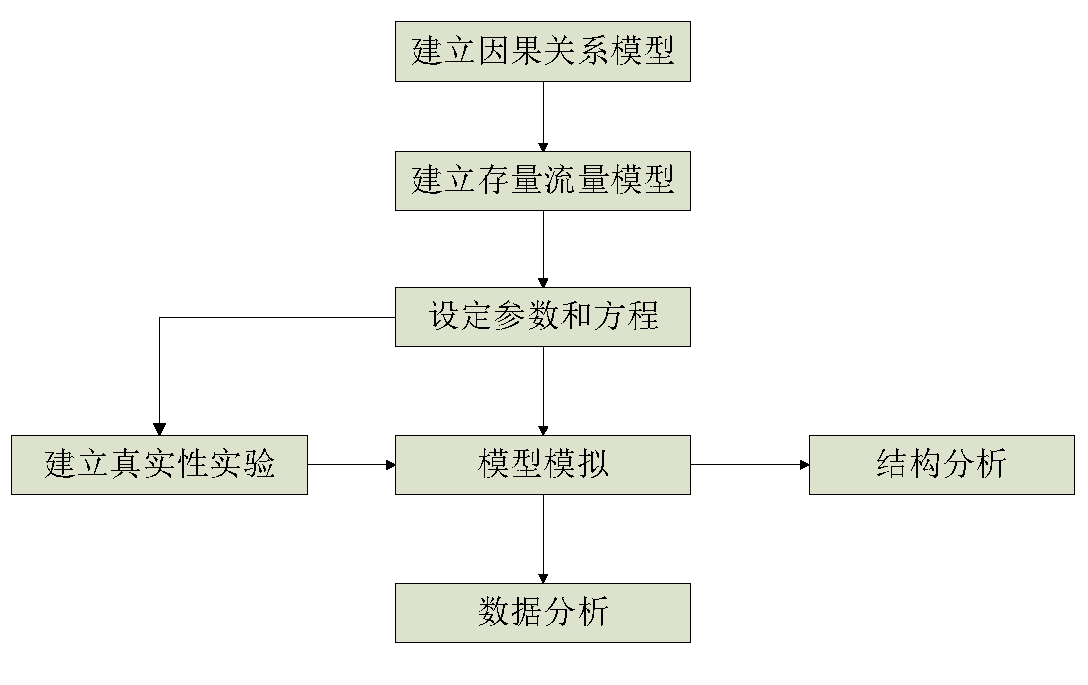
\includegraphics{vensim.pdf}}
  \caption{\small{\textbf{模型仿真过程}}}
  \label{fig:vensim}
\end{figure}
\subsection{动机因素存量流量图}

在因果图中,不论是动机因素,还是个体的行为都是系统的状态,是存量。为了
描述动机于行为间的关系而故意忽略了一些流量变量和外生变量。但是,这些被
忽略的变量对于整个系统起到了重要作用,没有这些变量系统就不可能正确地表
示现实系统的运行。

对于大部分动机因素,它们和个体的行为之间构成了一个正反馈回路和一个负反
馈回路,既动机的
增强会提升个体的行为水平,如果协同行为的得到了他人的正反馈,则会提升个体的动
机;反之如果协同行为得到了他人的负反馈,个体的动机会受到伤害。对于现实
系统来说,有几个重要的变量未能包含在因果图中。首先,个体的协同行为水平
不仅受到动机的影响,还受到其他因素,尤其是个体工作能力的限制。无论个体怎么
提升协同水平,都不可能超过个体的最大工作能力。这就是所谓“增长的极限”。
个体的最大工作能力是行为水平的抑制因素,使得行为水平不可能无限制地增长
下去。其次,动机作为系统中的存量,必然要受到流量的影响。动机的流
入是从协同活动中获得的正反馈转化的动机,动机的流出则是协同活动中获得的
负反馈使动机削弱的数量。流入水平和流出水平综合决定了动机存量的变化。第
三,不论是动机转化为行为还是行为的结果反馈影响动机都不是线性过程。这种
变换也存在边际递减效应,动机的水平越高,每增加一单位动机所能引起的行为
水平的增加就越少。因此如果仅考虑行为与动机的互动关系的话,个体的动机应
该呈对数增长(或减弱),最后接近某个极大(小)值。最后,成就动机同其他
动机略有不同。成就动机促使个体参与某种活动从中获得成就感。成就感的提升
削弱成就需求。但是成就感有一种随时间自动削弱的属性,在没有任何外力介入
的情况下成就感将逐渐流失,从而提升了个体的成就需求,促使他们参与新的活
动重新获得成就感。流失速度的不同决定了不同人的行为模式,对于流失速度快
的人来说,他们从参与活动中所获得的成就感迅速减少,因此这些人表现为进取
精神非常强,不停地追逐新的目标来满足自己对成功的渴望。而流失速度慢的人则
会很长时间满足于自身取得的成就,表现为为止步不前,不愿接受新的挑战。

根据以上分析的结果,本文将把因果关系图转换为存量流量图,同时在模型中加
入新的变量,使模型更符合现实世界。因为转换的模型力图完整描述存量于流量
的关系,因此对因果关系进行了简化处理。变量间具体、详细的因果关系请参考
因果关系图。大部分的动机因素都有同样的特征:动机增加引起行为水平的提升;
如果行为得到正反馈则会促使动机也得到相应的提升,负反馈则会使动机减弱。。对于利他主义和感知到的意义两类动机由
于和行为之间是单向关系,行为的结果不会对这两个变量产生。影响。成就动机和认知失调两类动机有
各自的特点:成就动机根据满足感的变化而变化;认知失调的变化方向则和其他
因素相反,正反馈会减少认知失调水平,从而降低个体动机。在模型中引入了流量变量“每次协同行为增加的动机”表示
动机的流入,“他人对个体的协同行为减少的动机”表示动机的流出,以此表示
动机的动态性;引入变量“疲劳“和外生变量“个人工作的最大能力”构建行为
的负反馈闭环,反应行为水平受到抑制的特征。引入流量变量“满足感的流失”
反应满足感随时间减少的特点。转换的存量流量图如图
\ref{fig:refined-model}和图\ref{fig:refined-model2}所示。

\begin{figure}[!htb]
  \centering
  \scalebox{0.59}{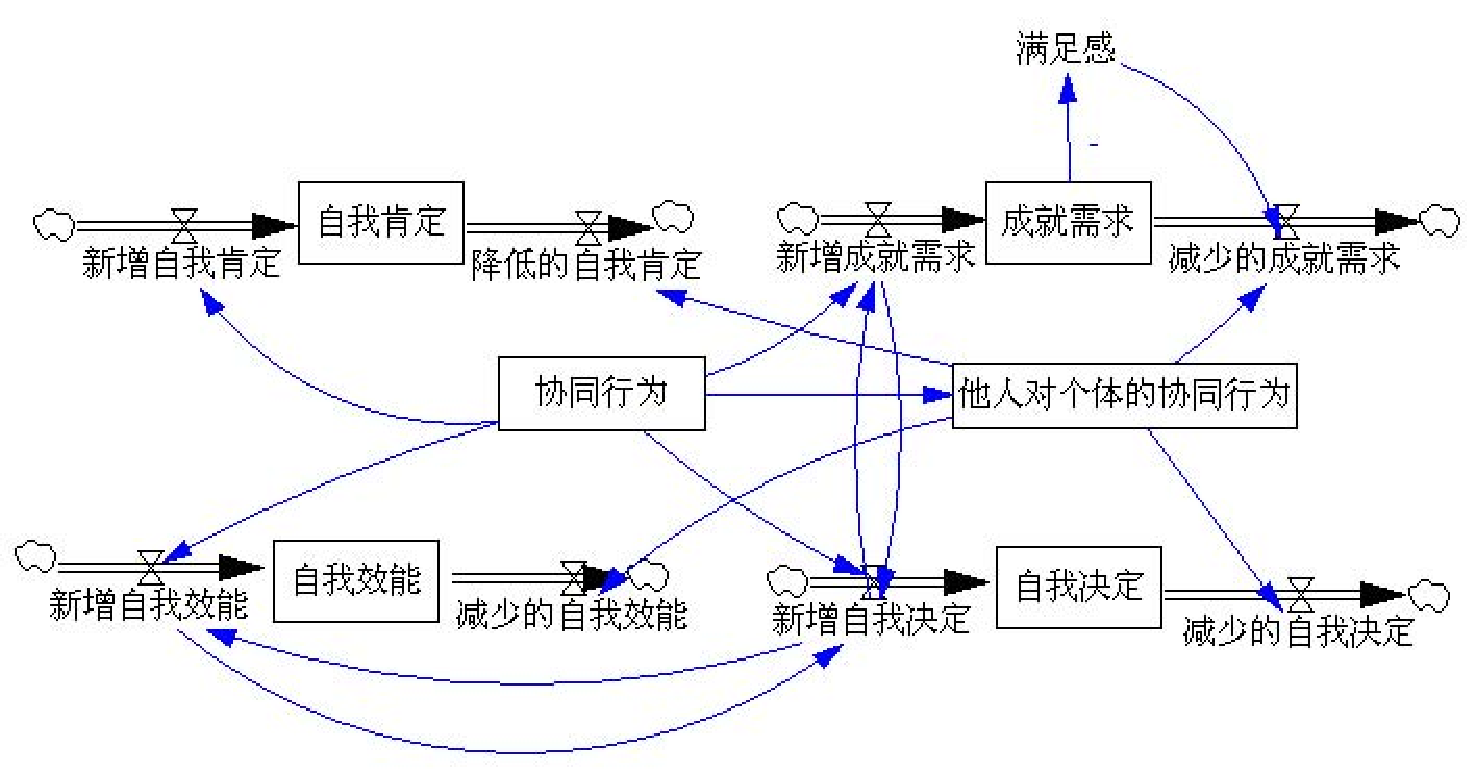
\includegraphics{io1.pdf}}
  \caption{\small{\textbf{知识协同个体动机因素的存量流量图}}}
  \label{fig:refined-model}
\end{figure}

\ref{fig:refined-model}所示。
\begin{figure}[!htb]
  \centering
  \scalebox{0.59}{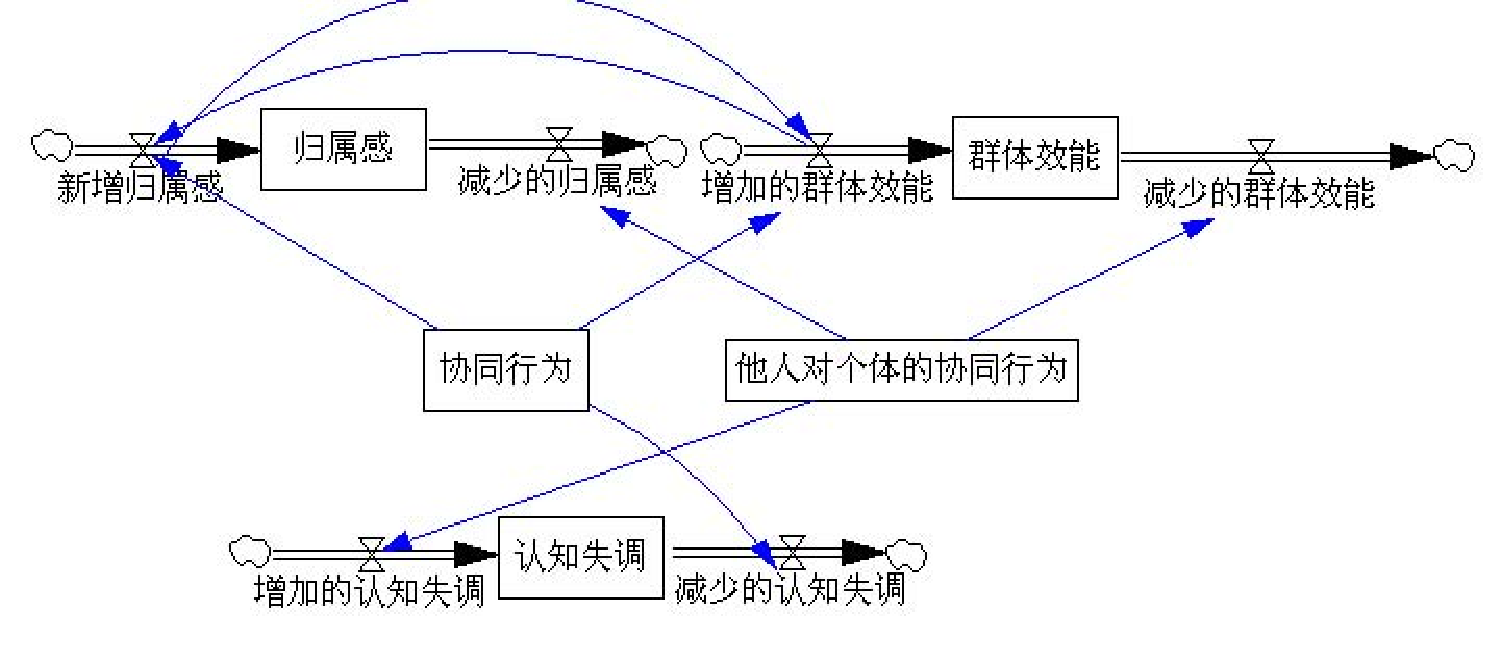
\includegraphics{io2.pdf}}
  \caption{\small{\textbf{知识协同人际间动机因素的存量流量图}}}
  \label{fig:refined-model2}
\end{figure}

\subsection{模型方程的设置}

每个变量都和其他变量形成一定的函数关系,这种关系使用方程来表示。下面列
举了模型中所有涉及到的方程。其中称领导者和领域专家的模型为模型1,内
容贡献者、维护者和边缘用户的模型为模型2.
\begin{enumerate}
\item 模型1行为水平=转换水平$_1$$\times (\sum$成就动机+利他主
  义+感知到的意义+自我决定+自我效能+自我肯定)
\item 模型2行为水平=转换水平$_1$$\times (\sum$成就动机+利他主
  义+感知到的意义+自我决定+自我效能+自我肯定+认知失调+群体效能+归属感)
  
\item 成就需求=个体的最大成就需求-满足感$\times$转换系数+本期自我决定
  增量$\times$转换系数
\item 自我决定=上一期自我决定+正协同贡献$\times$转换系数+负协同贡献
  $\times$转换系数+本期自我效能增量 $\times$转换系数+本期归属感增量$\times$转换系数
\item  自我效能=上一期自我效能+正协同贡献$\times$转换系数+负协同贡献
  $\times$转换系数+本期自我决定增量 $\times$转换系数
\item 自我肯定=上一期自我肯定+正协同贡献$\times$转换系数+负协同贡献
  $\times$转换系数
\item 认知失调=他人的协同行为$\times$转换系数+他人对个体的协同行为
  $\times$转换系数-协同行为水平$\times$转换系数
\item 群体效能=上一期群体效能定+正协同贡献$\times$转换系数+负协同贡献
  $\times$转换系数+本期归属感增量$\times$转换系数
\item 归属感=上一期归属感+正协同贡献$\times$转换系数+负协同贡献
  $\times$转换系数+本期自我效能增量 $\times$转换系数+本期群体效能增量 $\times$转换系数



\end{enumerate}

\subsection{参数估计}
参数估计是建立系统动力学模型重要的过程。即使是参数值的微小变化,也可能会引起系统
行为产生较大幅度的波动,甚至改变整个系统行为的极
性。因此, 为保证模型模拟结果与真实系统的一致性, 应尽可能地准确估计模型
的参数。

模型的参数估计是模型的局部分别独立地进行,然后在总体模型进行模拟仿真时
再进行总的调试。系统动力学本身并不限制参数估计的方法,可以根据需要和具
体情况灵活地选用不同的参数估计方法。参数估计的完成标志着模型从定性向定
量的转化。

参数的估计方法可以分为以下几种。
目前SD 模型参数估计的技术大致可分为3 种: (1) 单个参数、表函数关系、间接计算等基于利用
模型变量集结程度以下的数据进行的估计; (2) 运用单方程进行估计; (3) 运用多方程进行估计等. 其中后
2 种都是基于与模型变量集结程度相当的数据进行的估计. 此外, 还可以运用统计技术进行估计.
但是, SD 模型基于结构而不是统计相关性的特征, 使得它所要求的许多参数(如国民经济系统中描述
人均国民收入对积累率影响程度的参数等) 往往缺乏可资利用的资料, 使建模工作者可以有效地运用前述
的种种方法对它们进行合理的估计. 还有一种情况, 由于SD 模型所处理的常是具有多重反馈的复杂系
统, 这使得处在因果链上相隔甚远的变量间的关系变得很不直观甚至反直观, 要估计描述它们对应关系的
参数也十分困难. 为了对这些难以估计的参数进行估计, 有时就得采用“仿真—分析—修正”这种类似于手
工式的“试凑法'' \cite{linwenhao2002}。

参数的估计工作分为两部分,一部分是估计变量的初值,另一部分是估计方程中
的参数。在动机因素于协同行为的模型中,大部分变量都是定性变量,本身就难
于量化。在缺乏资料的情况下,将定性变量数量化,本身就带有一定的盲目性和
随意性,因此手工调试是必不可少的环节。但是,通过使用一定的估计方法能大
大简化手工调试的工作量,减少调试的时间。

本文通过使用回归方法,首先给出参数的初始值。随后在此基础上利用遗传算法
逐步求精\cite{linwenhao2002},最终获得各变量的参数值。

参数估计的结果如表\ref{tab:initail-value-level}和表\ref{tab:initail-value-transe}所示。
\begin{table}[!htbp]
  \centering
\small
  \caption{\small{\textbf{状态变量参数初始值}}}
% Table generated by Excel2LaTeX from sheet 'Sheet2'
\begin{tabular}{|c|c|c|c|c|c|}
\hline
\multicolumn{ 1}{|c|}{变量名称} &                                     \multicolumn{ 5}{|c|}{初始值} \\
\hline
\multicolumn{ 1}{|c|}{} &        领导者 &       领域专家 &      内容贡献者 &      内容维护者 &       边缘用户 \\
\hline
      利他主义 &      13      &        13    &        10    &   10         &      10      \\
\hline
    感知到的意义 &      10      &     10       &     10       &   10         &      10      \\
\hline
      自我决定 &      20      &     18       &      15      &          10  &    10        \\
\hline
      自我效能 &     25       &      15      &        15    &        8    &       5     \\
\hline
      自我肯定 &      25      &    15        &     10       &      10      &       10     \\
\hline
      成就需求 &     20       &     18       &      18      &      5      &        5    \\
\hline
      认知失调 &     $\slash$       &       $\slash$       &      10      &       15     &      9      \\
\hline
      群体效能 &     $\slash$         &          $\slash$    &    15        &      10      &       5     \\
\hline
       归属感 &       $\slash$       &     $\slash$         &      18      &        18    &        5    \\\hline
\end{tabular}  


  \label{tab:initail-value-level}
\end{table}

\begin{table}[!htb]
  \centering
\caption{\small{\textbf{转换系数初始值}}}
\small
% Table generated by Excel2LaTeX from sheet 'Sheet2'
\begin{tabular}{|c|c|c|c|c|c|}
\hline
\multicolumn{ 1}{|c|}{变量名称} &                                     \multicolumn{ 5}{|c|}{初始值} \\
\hline
\multicolumn{ 1}{|c|}{} &        领导者 &       领域专家 &      内容贡献者 &      内容维护者 &       边缘用户 \\
\hline
自我决定到协同水平的转换系数 &     0.003       &     0.003       &      0.002      &      0.001      &     0.001       \\
\hline
自我效能到协同水平的转换系数 &      0.005      &    0.005        &      0.006      &      0.008      &        0.008    \\
\hline
自我肯定到协同水平的转换系数 &      0.002     &       0.002    &      0.001      &     0.001       &       0.001     \\
\hline
成就需求到协同水平的转换系数 &     0.008       &     0.008       &     0.004       &         0.002   &       0.001     \\
\hline
认知失调到协同水平的转换系数 &      $\slash$       &    $\slash$         &    0.002        &         0.003   &      0.004      \\
\hline
群体效能到协同水平的转换系数 &          $\slash$    &       $\slash$       &   0.003         &    0.003        &        0.002    \\
\hline
归属感到协同水平的转换系数 &        $\slash$      &      $\slash$        &      0.003      &     0.003       &   0.003         \\
\hline
正协同贡献到自我决定的转换系数 &    0.0015        &    0.0014        &      0.0009      &        0.0006    &      0.0006      \\
\hline
正协同贡献到自我效能的转换系数 &    0.0022        &      0.0018      &       0.0013     &       0.0009     &  0.0009          \\
\hline
正协同贡献到自我肯定的转换系数 &     0.0014       &        0.0013    &     0.001       &        0.0006    &     0.0006       \\
\hline
正协同贡献到成就需求的转换系数 &       0.0008     &        0.0008    &      0.001      &       0.0008     &       0.0008     \\
\hline
正协同贡献到认知失调的转换系数 &     $\slash$        &     $\slash$        &    0.0007        &     0.0005       &       0.0006     \\
\hline
正协同贡献到群体效能的转换系数 &   $\slash$          &   $\slash$          &      0.0005      &     0.0005       &      0.0003      \\
\hline
正协同贡献到归属感的转换系数 &    $\slash$         &      $\slash$       &       0.0004     &      0.0005      &      0.0002      \\
\hline
负协同贡献到自我决定的转换系数 &     0.0001       &     0.0001       &    0.0005        &      0.0008      &     0.0009       \\
\hline
负协同贡献到自我效能的转换系数 &      0.0001      &     0.0001       &    0.0004        &      0.0009      &        0.001    \\
\hline
负协同贡献到自我肯定的转换系数 &     0.0001       &      0.0001
&0.0005&  0.0006            &  0.0006          \\
\hline
负协同贡献到成就需求的转换系数 &      0.0002      &       0.0002     &     0.0003       &       0.0003     &      0.0003      \\
\hline
负协同贡献到认知失调的转换系数 &       $\slash$      &    $\slash$         &    0.0002        &     0.0002       &     0.0001       \\
\hline
负协同贡献到群体效能的转换系数 &   $\slash$          &       $\slash$      &    0.0002        &       0.0002     &    0.0002        \\
\hline
负协同贡献到归属感的转换系数 &      $\slash$       &       $\slash$      &      0.0001      &        0.0003    &      0.0003      \\
\hline
\end{tabular}  

  
  \label{tab:initail-value-transe}
\end{table}

\section{模型检验}

当模型的所有参数都确定后,需要测试模型的有效性,检查模型是否能较准确地
模拟现实系统。模型的检验是一个不断证伪的过程。常见的检验方法包括结构评
价测试、参数估计测试、行为重现测试、灵敏度测试、系统改进测试等。检验往
往是通过同用户、专家的不断对话,深入理解系统行为,同时检查系统的因果关
系是否合理,方程量纲是否一致,对模型进行各种条件下的测试,并对比模型的
运行结果和实际数据。本文在参考大量文献的基础上,借鉴了其他学者的实证研
究成果,对模型进行历史检验,把模拟结果与历史数据进行
对照和比较, 以验证模型与客观系统的吻合程度, 从而判
定模型能否有效地反映客观系统,既观测模型是否能重现真实系统中的行为变化。
同时,对模型进行灵敏度检验,观测参数变化对于模型的影响。



模型是现实世界的简化和抽象,因此一个模型不可能精确地再现现实中的各种现
象。模型的主要目的在于反映趋势的变化。为了验证模型的正确性,本文将模型
仿真数据同真实数据进行对比。针对不同类型的用户,使用维基百科提供的数据分别计算了连续40个月的
月人均贡献度和仿真结果进行比对。

图\ref{fig:simu1}是领导者用户的仿真结果和真实数据图。从图中可以看出,领导者用户的月人
均贡献度呈现出比较明显的对数函数特征,而仿真的结果显示为系统行为呈现出
寻的模式,因此虽然模型同实际数据有误差,但是仍然较准确地再现了现实趋
势,可以使用模型模拟用户的知识协同行为。

\begin{figure}[!htb]
  \centering
 % \scalebox{0.65}{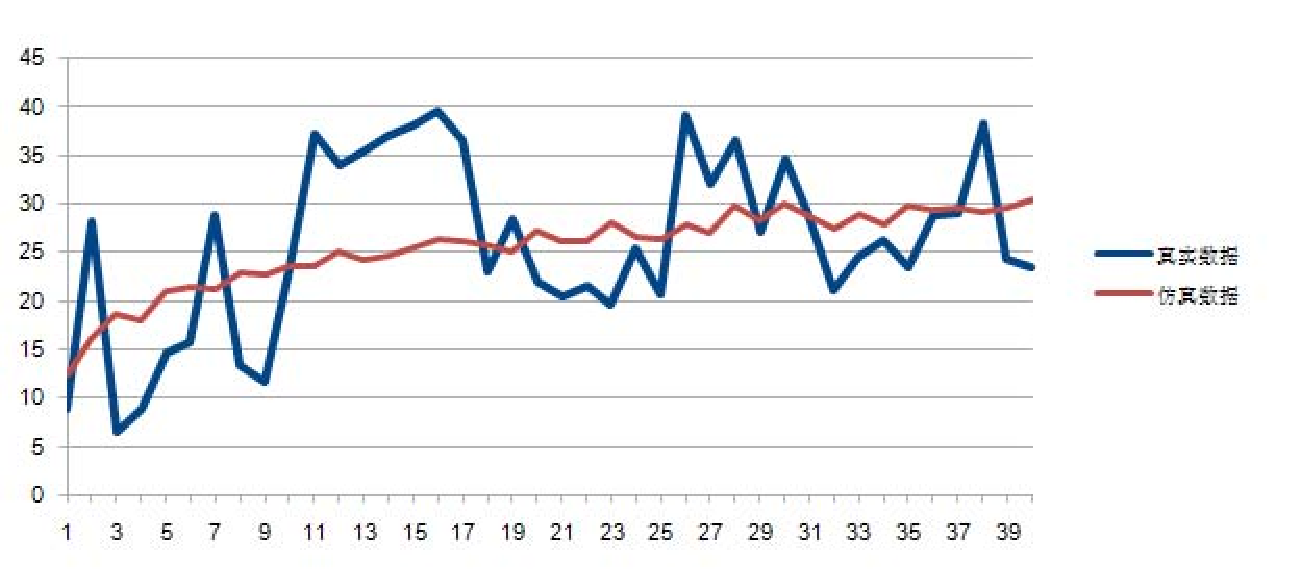
\includegraphics{simu-1.pdf}}
% GNUPLOT: LaTeX picture
\setlength{\unitlength}{0.240900pt}
\ifx\plotpoint\undefined\newsavebox{\plotpoint}\fi
\begin{picture}(1500,900)(0,0)
\sbox{\plotpoint}{\rule[-0.200pt]{0.400pt}{0.400pt}}%
\put(131.0,204.0){\rule[-0.200pt]{4.818pt}{0.400pt}}
\put(111,204){\makebox(0,0)[r]{5}}
\put(1419.0,204.0){\rule[-0.200pt]{4.818pt}{0.400pt}}
\put(131.0,277.0){\rule[-0.200pt]{4.818pt}{0.400pt}}
\put(111,277){\makebox(0,0)[r]{10}}
\put(1419.0,277.0){\rule[-0.200pt]{4.818pt}{0.400pt}}
\put(131.0,349.0){\rule[-0.200pt]{4.818pt}{0.400pt}}
\put(111,349){\makebox(0,0)[r]{15}}
\put(1419.0,349.0){\rule[-0.200pt]{4.818pt}{0.400pt}}
\put(131.0,422.0){\rule[-0.200pt]{4.818pt}{0.400pt}}
\put(111,422){\makebox(0,0)[r]{20}}
\put(1419.0,422.0){\rule[-0.200pt]{4.818pt}{0.400pt}}
\put(131.0,495.0){\rule[-0.200pt]{4.818pt}{0.400pt}}
\put(111,495){\makebox(0,0)[r]{25}}
\put(1419.0,495.0){\rule[-0.200pt]{4.818pt}{0.400pt}}
\put(131.0,568.0){\rule[-0.200pt]{4.818pt}{0.400pt}}
\put(111,568){\makebox(0,0)[r]{30}}
\put(1419.0,568.0){\rule[-0.200pt]{4.818pt}{0.400pt}}
\put(131.0,641.0){\rule[-0.200pt]{4.818pt}{0.400pt}}
\put(111,641){\makebox(0,0)[r]{35}}
\put(1419.0,641.0){\rule[-0.200pt]{4.818pt}{0.400pt}}
\put(131.0,713.0){\rule[-0.200pt]{4.818pt}{0.400pt}}
\put(111,713){\makebox(0,0)[r]{40}}
\put(1419.0,713.0){\rule[-0.200pt]{4.818pt}{0.400pt}}
\put(164.0,131.0){\rule[-0.200pt]{0.400pt}{4.818pt}}
\put(164,90){\makebox(0,0){ 1}}
\put(164.0,839.0){\rule[-0.200pt]{0.400pt}{4.818pt}}
\put(229.0,131.0){\rule[-0.200pt]{0.400pt}{4.818pt}}
\put(229,90){\makebox(0,0){ 3}}
\put(229.0,839.0){\rule[-0.200pt]{0.400pt}{4.818pt}}
\put(295.0,131.0){\rule[-0.200pt]{0.400pt}{4.818pt}}
\put(295,90){\makebox(0,0){ 5}}
\put(295.0,839.0){\rule[-0.200pt]{0.400pt}{4.818pt}}
\put(360.0,131.0){\rule[-0.200pt]{0.400pt}{4.818pt}}
\put(360,90){\makebox(0,0){ 7}}
\put(360.0,839.0){\rule[-0.200pt]{0.400pt}{4.818pt}}
\put(425.0,131.0){\rule[-0.200pt]{0.400pt}{4.818pt}}
\put(425,90){\makebox(0,0){ 9}}
\put(425.0,839.0){\rule[-0.200pt]{0.400pt}{4.818pt}}
\put(491.0,131.0){\rule[-0.200pt]{0.400pt}{4.818pt}}
\put(491,90){\makebox(0,0){ 11}}
\put(491.0,839.0){\rule[-0.200pt]{0.400pt}{4.818pt}}
\put(556.0,131.0){\rule[-0.200pt]{0.400pt}{4.818pt}}
\put(556,90){\makebox(0,0){ 13}}
\put(556.0,839.0){\rule[-0.200pt]{0.400pt}{4.818pt}}
\put(622.0,131.0){\rule[-0.200pt]{0.400pt}{4.818pt}}
\put(622,90){\makebox(0,0){ 15}}
\put(622.0,839.0){\rule[-0.200pt]{0.400pt}{4.818pt}}
\put(687.0,131.0){\rule[-0.200pt]{0.400pt}{4.818pt}}
\put(687,90){\makebox(0,0){ 17}}
\put(687.0,839.0){\rule[-0.200pt]{0.400pt}{4.818pt}}
\put(752.0,131.0){\rule[-0.200pt]{0.400pt}{4.818pt}}
\put(752,90){\makebox(0,0){ 19}}
\put(752.0,839.0){\rule[-0.200pt]{0.400pt}{4.818pt}}
\put(818.0,131.0){\rule[-0.200pt]{0.400pt}{4.818pt}}
\put(818,90){\makebox(0,0){ 21}}
\put(818.0,839.0){\rule[-0.200pt]{0.400pt}{4.818pt}}
\put(883.0,131.0){\rule[-0.200pt]{0.400pt}{4.818pt}}
\put(883,90){\makebox(0,0){ 23}}
\put(883.0,839.0){\rule[-0.200pt]{0.400pt}{4.818pt}}
\put(949.0,131.0){\rule[-0.200pt]{0.400pt}{4.818pt}}
\put(949,90){\makebox(0,0){ 25}}
\put(949.0,839.0){\rule[-0.200pt]{0.400pt}{4.818pt}}
\put(1014.0,131.0){\rule[-0.200pt]{0.400pt}{4.818pt}}
\put(1014,90){\makebox(0,0){ 27}}
\put(1014.0,839.0){\rule[-0.200pt]{0.400pt}{4.818pt}}
\put(1079.0,131.0){\rule[-0.200pt]{0.400pt}{4.818pt}}
\put(1079,90){\makebox(0,0){ 29}}
\put(1079.0,839.0){\rule[-0.200pt]{0.400pt}{4.818pt}}
\put(1145.0,131.0){\rule[-0.200pt]{0.400pt}{4.818pt}}
\put(1145,90){\makebox(0,0){ 31}}
\put(1145.0,839.0){\rule[-0.200pt]{0.400pt}{4.818pt}}
\put(1210.0,131.0){\rule[-0.200pt]{0.400pt}{4.818pt}}
\put(1210,90){\makebox(0,0){ 33}}
\put(1210.0,839.0){\rule[-0.200pt]{0.400pt}{4.818pt}}
\put(1276.0,131.0){\rule[-0.200pt]{0.400pt}{4.818pt}}
\put(1276,90){\makebox(0,0){ 35}}
\put(1276.0,839.0){\rule[-0.200pt]{0.400pt}{4.818pt}}
\put(1341.0,131.0){\rule[-0.200pt]{0.400pt}{4.818pt}}
\put(1341,90){\makebox(0,0){ 37}}
\put(1341.0,839.0){\rule[-0.200pt]{0.400pt}{4.818pt}}
\put(1406.0,131.0){\rule[-0.200pt]{0.400pt}{4.818pt}}
\put(1406,90){\makebox(0,0){ 39}}
\put(1406.0,839.0){\rule[-0.200pt]{0.400pt}{4.818pt}}
\put(131.0,131.0){\rule[-0.200pt]{0.400pt}{175.375pt}}
\put(131.0,131.0){\rule[-0.200pt]{315.097pt}{0.400pt}}
\put(1439.0,131.0){\rule[-0.200pt]{0.400pt}{175.375pt}}
\put(131.0,859.0){\rule[-0.200pt]{315.097pt}{0.400pt}}
\put(30,495){\makebox(0,0){\rotatebox{90}{用户贡献}}}
\put(785,29){\makebox(0,0){}}
\sbox{\plotpoint}{\rule[-0.400pt]{0.800pt}{0.800pt}}%
\sbox{\plotpoint}{\rule[-0.200pt]{0.400pt}{0.400pt}}%
\put(1279,819){\makebox(0,0)[r]{仿真数据}}
\sbox{\plotpoint}{\rule[-0.400pt]{0.800pt}{0.800pt}}%
\put(1299.0,819.0){\rule[-0.400pt]{24.090pt}{0.800pt}}
\put(164,309){\usebox{\plotpoint}}
\multiput(165.41,309.00)(0.503,0.785){57}{\rule{0.121pt}{1.450pt}}
\multiput(162.34,309.00)(32.000,46.990){2}{\rule{0.800pt}{0.725pt}}
\multiput(196.00,360.41)(0.568,0.504){51}{\rule{1.110pt}{0.121pt}}
\multiput(196.00,357.34)(30.695,29.000){2}{\rule{0.555pt}{0.800pt}}
\multiput(229.00,389.41)(0.793,0.505){35}{\rule{1.457pt}{0.122pt}}
\multiput(229.00,386.34)(29.976,21.000){2}{\rule{0.729pt}{0.800pt}}
\multiput(262.00,410.41)(1.055,0.507){25}{\rule{1.850pt}{0.122pt}}
\multiput(262.00,407.34)(29.160,16.000){2}{\rule{0.925pt}{0.800pt}}
\multiput(295.00,426.41)(1.278,0.509){19}{\rule{2.169pt}{0.123pt}}
\multiput(295.00,423.34)(27.498,13.000){2}{\rule{1.085pt}{0.800pt}}
\multiput(327.00,439.40)(1.586,0.512){15}{\rule{2.600pt}{0.123pt}}
\multiput(327.00,436.34)(27.604,11.000){2}{\rule{1.300pt}{0.800pt}}
\multiput(360.00,450.40)(1.768,0.514){13}{\rule{2.840pt}{0.124pt}}
\multiput(360.00,447.34)(27.105,10.000){2}{\rule{1.420pt}{0.800pt}}
\multiput(393.00,460.40)(1.936,0.516){11}{\rule{3.044pt}{0.124pt}}
\multiput(393.00,457.34)(25.681,9.000){2}{\rule{1.522pt}{0.800pt}}
\multiput(425.00,469.40)(2.752,0.526){7}{\rule{3.971pt}{0.127pt}}
\multiput(425.00,466.34)(24.757,7.000){2}{\rule{1.986pt}{0.800pt}}
\multiput(458.00,476.40)(2.752,0.526){7}{\rule{3.971pt}{0.127pt}}
\multiput(458.00,473.34)(24.757,7.000){2}{\rule{1.986pt}{0.800pt}}
\multiput(491.00,483.39)(3.365,0.536){5}{\rule{4.467pt}{0.129pt}}
\multiput(491.00,480.34)(22.729,6.000){2}{\rule{2.233pt}{0.800pt}}
\multiput(523.00,489.39)(3.476,0.536){5}{\rule{4.600pt}{0.129pt}}
\multiput(523.00,486.34)(23.452,6.000){2}{\rule{2.300pt}{0.800pt}}
\multiput(556.00,495.39)(3.476,0.536){5}{\rule{4.600pt}{0.129pt}}
\multiput(556.00,492.34)(23.452,6.000){2}{\rule{2.300pt}{0.800pt}}
\multiput(589.00,501.38)(5.126,0.560){3}{\rule{5.480pt}{0.135pt}}
\multiput(589.00,498.34)(21.626,5.000){2}{\rule{2.740pt}{0.800pt}}
\put(622,505.34){\rule{6.600pt}{0.800pt}}
\multiput(622.00,503.34)(18.301,4.000){2}{\rule{3.300pt}{0.800pt}}
\multiput(654.00,510.38)(5.126,0.560){3}{\rule{5.480pt}{0.135pt}}
\multiput(654.00,507.34)(21.626,5.000){2}{\rule{2.740pt}{0.800pt}}
\put(687,514.34){\rule{6.800pt}{0.800pt}}
\multiput(687.00,512.34)(18.886,4.000){2}{\rule{3.400pt}{0.800pt}}
\put(720,518.34){\rule{6.600pt}{0.800pt}}
\multiput(720.00,516.34)(18.301,4.000){2}{\rule{3.300pt}{0.800pt}}
\put(752,521.84){\rule{7.950pt}{0.800pt}}
\multiput(752.00,520.34)(16.500,3.000){2}{\rule{3.975pt}{0.800pt}}
\put(785,525.34){\rule{6.800pt}{0.800pt}}
\multiput(785.00,523.34)(18.886,4.000){2}{\rule{3.400pt}{0.800pt}}
\put(818,528.84){\rule{7.709pt}{0.800pt}}
\multiput(818.00,527.34)(16.000,3.000){2}{\rule{3.854pt}{0.800pt}}
\put(850,532.34){\rule{6.800pt}{0.800pt}}
\multiput(850.00,530.34)(18.886,4.000){2}{\rule{3.400pt}{0.800pt}}
\put(883,535.84){\rule{7.950pt}{0.800pt}}
\multiput(883.00,534.34)(16.500,3.000){2}{\rule{3.975pt}{0.800pt}}
\put(916,538.84){\rule{7.950pt}{0.800pt}}
\multiput(916.00,537.34)(16.500,3.000){2}{\rule{3.975pt}{0.800pt}}
\put(949,541.34){\rule{7.709pt}{0.800pt}}
\multiput(949.00,540.34)(16.000,2.000){2}{\rule{3.854pt}{0.800pt}}
\put(981,543.84){\rule{7.950pt}{0.800pt}}
\multiput(981.00,542.34)(16.500,3.000){2}{\rule{3.975pt}{0.800pt}}
\put(1014,546.84){\rule{7.950pt}{0.800pt}}
\multiput(1014.00,545.34)(16.500,3.000){2}{\rule{3.975pt}{0.800pt}}
\put(1047,549.34){\rule{7.709pt}{0.800pt}}
\multiput(1047.00,548.34)(16.000,2.000){2}{\rule{3.854pt}{0.800pt}}
\put(1079,551.84){\rule{7.950pt}{0.800pt}}
\multiput(1079.00,550.34)(16.500,3.000){2}{\rule{3.975pt}{0.800pt}}
\put(1112,554.34){\rule{7.950pt}{0.800pt}}
\multiput(1112.00,553.34)(16.500,2.000){2}{\rule{3.975pt}{0.800pt}}
\put(1145,556.84){\rule{7.709pt}{0.800pt}}
\multiput(1145.00,555.34)(16.000,3.000){2}{\rule{3.854pt}{0.800pt}}
\put(1177,559.34){\rule{7.950pt}{0.800pt}}
\multiput(1177.00,558.34)(16.500,2.000){2}{\rule{3.975pt}{0.800pt}}
\put(1210,561.34){\rule{7.950pt}{0.800pt}}
\multiput(1210.00,560.34)(16.500,2.000){2}{\rule{3.975pt}{0.800pt}}
\put(1243,563.34){\rule{7.950pt}{0.800pt}}
\multiput(1243.00,562.34)(16.500,2.000){2}{\rule{3.975pt}{0.800pt}}
\put(1276,565.34){\rule{7.709pt}{0.800pt}}
\multiput(1276.00,564.34)(16.000,2.000){2}{\rule{3.854pt}{0.800pt}}
\put(1308,567.34){\rule{7.950pt}{0.800pt}}
\multiput(1308.00,566.34)(16.500,2.000){2}{\rule{3.975pt}{0.800pt}}
\put(1341,569.34){\rule{7.950pt}{0.800pt}}
\multiput(1341.00,568.34)(16.500,2.000){2}{\rule{3.975pt}{0.800pt}}
\put(1374,571.34){\rule{7.709pt}{0.800pt}}
\multiput(1374.00,570.34)(16.000,2.000){2}{\rule{3.854pt}{0.800pt}}
\put(1406,573.34){\rule{7.950pt}{0.800pt}}
\multiput(1406.00,572.34)(16.500,2.000){2}{\rule{3.975pt}{0.800pt}}
\sbox{\plotpoint}{\rule[-0.200pt]{0.400pt}{0.400pt}}%
\put(1279,769){\makebox(0,0)[r]{实际数据}}
\put(1299.0,778.0){\rule[-0.200pt]{24.090pt}{0.400pt}}
\put(164,260){\usebox{\plotpoint}}
\multiput(164.58,260.00)(0.497,4.449){61}{\rule{0.120pt}{3.625pt}}
\multiput(163.17,260.00)(32.000,274.476){2}{\rule{0.400pt}{1.813pt}}
\multiput(196.58,533.03)(0.497,-2.597){63}{\rule{0.120pt}{2.161pt}}
\multiput(195.17,537.52)(33.000,-165.516){2}{\rule{0.400pt}{1.080pt}}
\multiput(229.58,372.00)(0.497,0.514){63}{\rule{0.120pt}{0.512pt}}
\multiput(228.17,372.00)(33.000,32.937){2}{\rule{0.400pt}{0.256pt}}
\multiput(262.58,402.52)(0.497,-0.928){63}{\rule{0.120pt}{0.839pt}}
\multiput(261.17,404.26)(33.000,-59.258){2}{\rule{0.400pt}{0.420pt}}
\multiput(295.00,345.58)(1.009,0.494){29}{\rule{0.900pt}{0.119pt}}
\multiput(295.00,344.17)(30.132,16.000){2}{\rule{0.450pt}{0.400pt}}
\multiput(327.58,361.00)(0.497,2.919){63}{\rule{0.120pt}{2.415pt}}
\multiput(326.17,361.00)(33.000,185.987){2}{\rule{0.400pt}{1.208pt}}
\multiput(360.58,543.94)(0.497,-2.322){63}{\rule{0.120pt}{1.942pt}}
\multiput(359.17,547.97)(33.000,-147.968){2}{\rule{0.400pt}{0.971pt}}
\multiput(393.58,400.00)(0.497,0.736){61}{\rule{0.120pt}{0.688pt}}
\multiput(392.17,400.00)(32.000,45.573){2}{\rule{0.400pt}{0.344pt}}
\multiput(425.00,447.58)(0.661,0.497){47}{\rule{0.628pt}{0.120pt}}
\multiput(425.00,446.17)(31.697,25.000){2}{\rule{0.314pt}{0.400pt}}
\multiput(458.58,472.00)(0.497,0.820){63}{\rule{0.120pt}{0.755pt}}
\multiput(457.17,472.00)(33.000,52.434){2}{\rule{0.400pt}{0.377pt}}
\multiput(491.58,526.00)(0.497,1.542){61}{\rule{0.120pt}{1.325pt}}
\multiput(490.17,526.00)(32.000,95.250){2}{\rule{0.400pt}{0.663pt}}
\multiput(523.58,621.87)(0.497,-0.514){63}{\rule{0.120pt}{0.512pt}}
\multiput(522.17,622.94)(33.000,-32.937){2}{\rule{0.400pt}{0.256pt}}
\multiput(556.00,590.58)(0.752,0.496){41}{\rule{0.700pt}{0.120pt}}
\multiput(556.00,589.17)(31.547,22.000){2}{\rule{0.350pt}{0.400pt}}
\multiput(589.00,610.92)(0.549,-0.497){57}{\rule{0.540pt}{0.120pt}}
\multiput(589.00,611.17)(31.879,-30.000){2}{\rule{0.270pt}{0.400pt}}
\multiput(622.00,580.93)(2.841,-0.482){9}{\rule{2.233pt}{0.116pt}}
\multiput(622.00,581.17)(27.365,-6.000){2}{\rule{1.117pt}{0.400pt}}
\multiput(654.58,576.00)(0.497,0.652){63}{\rule{0.120pt}{0.621pt}}
\multiput(653.17,576.00)(33.000,41.711){2}{\rule{0.400pt}{0.311pt}}
\multiput(687.58,612.40)(0.497,-1.877){63}{\rule{0.120pt}{1.591pt}}
\multiput(686.17,615.70)(33.000,-119.698){2}{\rule{0.400pt}{0.795pt}}
\multiput(720.58,496.00)(0.497,0.752){61}{\rule{0.120pt}{0.700pt}}
\multiput(719.17,496.00)(32.000,46.547){2}{\rule{0.400pt}{0.350pt}}
\multiput(752.00,542.93)(2.476,-0.485){11}{\rule{1.986pt}{0.117pt}}
\multiput(752.00,543.17)(28.879,-7.000){2}{\rule{0.993pt}{0.400pt}}
\multiput(785.58,534.77)(0.497,-0.545){63}{\rule{0.120pt}{0.536pt}}
\multiput(784.17,535.89)(33.000,-34.887){2}{\rule{0.400pt}{0.268pt}}
\multiput(818.00,501.58)(1.009,0.494){29}{\rule{0.900pt}{0.119pt}}
\multiput(818.00,500.17)(30.132,16.000){2}{\rule{0.450pt}{0.400pt}}
\multiput(850.00,515.92)(0.589,-0.497){53}{\rule{0.571pt}{0.120pt}}
\multiput(850.00,516.17)(31.814,-28.000){2}{\rule{0.286pt}{0.400pt}}
\multiput(883.00,489.58)(1.290,0.493){23}{\rule{1.115pt}{0.119pt}}
\multiput(883.00,488.17)(30.685,13.000){2}{\rule{0.558pt}{0.400pt}}
\multiput(916.58,502.00)(0.497,0.912){63}{\rule{0.120pt}{0.827pt}}
\multiput(915.17,502.00)(33.000,58.283){2}{\rule{0.400pt}{0.414pt}}
\multiput(949.58,562.00)(0.497,1.036){61}{\rule{0.120pt}{0.925pt}}
\multiput(948.17,562.00)(32.000,64.080){2}{\rule{0.400pt}{0.463pt}}
\multiput(981.00,626.92)(0.549,-0.497){57}{\rule{0.540pt}{0.120pt}}
\multiput(981.00,627.17)(31.879,-30.000){2}{\rule{0.270pt}{0.400pt}}
\multiput(1014.00,596.93)(2.476,-0.485){11}{\rule{1.986pt}{0.117pt}}
\multiput(1014.00,597.17)(28.879,-7.000){2}{\rule{0.993pt}{0.400pt}}
\multiput(1047.58,587.21)(0.497,-1.020){61}{\rule{0.120pt}{0.913pt}}
\multiput(1046.17,589.11)(32.000,-63.106){2}{\rule{0.400pt}{0.456pt}}
\multiput(1079.58,526.00)(0.497,1.663){63}{\rule{0.120pt}{1.421pt}}
\multiput(1078.17,526.00)(33.000,106.050){2}{\rule{0.400pt}{0.711pt}}
\multiput(1112.58,630.41)(0.497,-1.265){63}{\rule{0.120pt}{1.106pt}}
\multiput(1111.17,632.70)(33.000,-80.704){2}{\rule{0.400pt}{0.553pt}}
\multiput(1145.58,552.00)(0.497,0.515){61}{\rule{0.120pt}{0.512pt}}
\multiput(1144.17,552.00)(32.000,31.936){2}{\rule{0.400pt}{0.256pt}}
\multiput(1177.58,585.00)(0.497,0.744){63}{\rule{0.120pt}{0.694pt}}
\multiput(1176.17,585.00)(33.000,47.560){2}{\rule{0.400pt}{0.347pt}}
\multiput(1210.58,627.45)(0.497,-1.862){63}{\rule{0.120pt}{1.579pt}}
\multiput(1209.17,630.72)(33.000,-118.723){2}{\rule{0.400pt}{0.789pt}}
\multiput(1243.58,512.00)(0.497,1.617){63}{\rule{0.120pt}{1.385pt}}
\multiput(1242.17,512.00)(33.000,103.126){2}{\rule{0.400pt}{0.692pt}}
\multiput(1276.58,614.06)(0.497,-1.068){61}{\rule{0.120pt}{0.950pt}}
\multiput(1275.17,616.03)(32.000,-66.028){2}{\rule{0.400pt}{0.475pt}}
\multiput(1308.00,550.59)(3.604,0.477){7}{\rule{2.740pt}{0.115pt}}
\multiput(1308.00,549.17)(27.313,5.000){2}{\rule{1.370pt}{0.400pt}}
\multiput(1341.58,555.00)(0.497,1.586){63}{\rule{0.120pt}{1.361pt}}
\multiput(1340.17,555.00)(33.000,101.176){2}{\rule{0.400pt}{0.680pt}}
\multiput(1374.00,657.92)(0.551,-0.497){55}{\rule{0.541pt}{0.120pt}}
\multiput(1374.00,658.17)(30.876,-29.000){2}{\rule{0.271pt}{0.400pt}}
\multiput(1406.00,628.92)(1.290,-0.493){23}{\rule{1.115pt}{0.119pt}}
\multiput(1406.00,629.17)(30.685,-13.000){2}{\rule{0.558pt}{0.400pt}}
\put(164,260){\makebox(0,0){$+$}}
\put(196,542){\makebox(0,0){$+$}}
\put(229,372){\makebox(0,0){$+$}}
\put(262,406){\makebox(0,0){$+$}}
\put(295,345){\makebox(0,0){$+$}}
\put(327,361){\makebox(0,0){$+$}}
\put(360,552){\makebox(0,0){$+$}}
\put(393,400){\makebox(0,0){$+$}}
\put(425,447){\makebox(0,0){$+$}}
\put(458,472){\makebox(0,0){$+$}}
\put(491,526){\makebox(0,0){$+$}}
\put(523,624){\makebox(0,0){$+$}}
\put(556,590){\makebox(0,0){$+$}}
\put(589,612){\makebox(0,0){$+$}}
\put(622,582){\makebox(0,0){$+$}}
\put(654,576){\makebox(0,0){$+$}}
\put(687,619){\makebox(0,0){$+$}}
\put(720,496){\makebox(0,0){$+$}}
\put(752,544){\makebox(0,0){$+$}}
\put(785,537){\makebox(0,0){$+$}}
\put(818,501){\makebox(0,0){$+$}}
\put(850,517){\makebox(0,0){$+$}}
\put(883,489){\makebox(0,0){$+$}}
\put(916,502){\makebox(0,0){$+$}}
\put(949,562){\makebox(0,0){$+$}}
\put(981,628){\makebox(0,0){$+$}}
\put(1014,598){\makebox(0,0){$+$}}
\put(1047,591){\makebox(0,0){$+$}}
\put(1079,526){\makebox(0,0){$+$}}
\put(1112,635){\makebox(0,0){$+$}}
\put(1145,552){\makebox(0,0){$+$}}
\put(1177,585){\makebox(0,0){$+$}}
\put(1210,634){\makebox(0,0){$+$}}
\put(1243,512){\makebox(0,0){$+$}}
\put(1276,618){\makebox(0,0){$+$}}
\put(1308,550){\makebox(0,0){$+$}}
\put(1341,555){\makebox(0,0){$+$}}
\put(1374,659){\makebox(0,0){$+$}}
\put(1406,630){\makebox(0,0){$+$}}
\put(1439,617){\makebox(0,0){$+$}}
\put(1349,778){\makebox(0,0){$+$}}
\put(131.0,131.0){\rule[-0.200pt]{0.400pt}{175.375pt}}
\put(131.0,131.0){\rule[-0.200pt]{315.097pt}{0.400pt}}
\put(1439.0,131.0){\rule[-0.200pt]{0.400pt}{175.375pt}}
\put(131.0,859.0){\rule[-0.200pt]{315.097pt}{0.400pt}}
\end{picture}
 
 \caption{\small{\textbf{领导者用户仿真结果}}}
  \label{fig:simu1}
\end{figure}

图\ref{fig:simu2}是领域专家用户的仿真结果和真实数据图。真实数据反映出该类用户的月人均
贡献度在初期显著下降后迅速进入一个平稳状态。仿真结果则表现为一个递减
的对数函数。两者的趋势是一致的。

\begin{figure}[!htb]
  \centering
%  \scalebox{0.65}{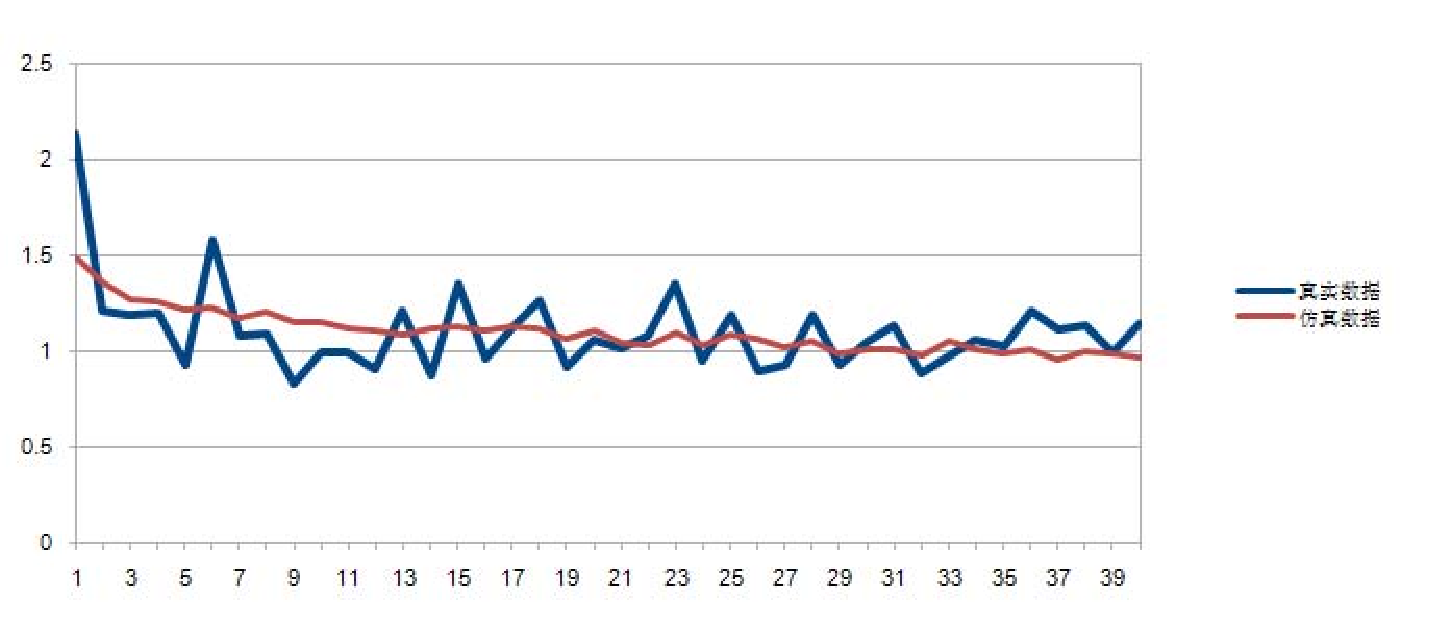
\includegraphics{simu-2.pdf}}
 % GNUPLOT: LaTeX picture
\setlength{\unitlength}{0.240900pt}
\ifx\plotpoint\undefined\newsavebox{\plotpoint}\fi
\begin{picture}(1500,900)(0,0)
\sbox{\plotpoint}{\rule[-0.200pt]{0.400pt}{0.400pt}}%
\put(131.0,82.0){\rule[-0.200pt]{4.818pt}{0.400pt}}
\put(111,82){\makebox(0,0)[r]{ 0}}
\put(1419.0,82.0){\rule[-0.200pt]{4.818pt}{0.400pt}}
\put(131.0,341.0){\rule[-0.200pt]{4.818pt}{0.400pt}}
\put(111,341){\makebox(0,0)[r]{ 1}}
\put(1419.0,341.0){\rule[-0.200pt]{4.818pt}{0.400pt}}
\put(131.0,600.0){\rule[-0.200pt]{4.818pt}{0.400pt}}
\put(111,600){\makebox(0,0)[r]{ 2}}
\put(1419.0,600.0){\rule[-0.200pt]{4.818pt}{0.400pt}}
\put(131.0,859.0){\rule[-0.200pt]{4.818pt}{0.400pt}}
\put(111,859){\makebox(0,0)[r]{ 3}}
\put(1419.0,859.0){\rule[-0.200pt]{4.818pt}{0.400pt}}
\put(131.0,82.0){\rule[-0.200pt]{0.400pt}{4.818pt}}
\put(131,41){\makebox(0,0){ 1}}
\put(131.0,839.0){\rule[-0.200pt]{0.400pt}{4.818pt}}
\put(198.0,82.0){\rule[-0.200pt]{0.400pt}{4.818pt}}
\put(198,41){\makebox(0,0){ 3}}
\put(198.0,839.0){\rule[-0.200pt]{0.400pt}{4.818pt}}
\put(265.0,82.0){\rule[-0.200pt]{0.400pt}{4.818pt}}
\put(265,41){\makebox(0,0){ 5}}
\put(265.0,839.0){\rule[-0.200pt]{0.400pt}{4.818pt}}
\put(332.0,82.0){\rule[-0.200pt]{0.400pt}{4.818pt}}
\put(332,41){\makebox(0,0){ 7}}
\put(332.0,839.0){\rule[-0.200pt]{0.400pt}{4.818pt}}
\put(399.0,82.0){\rule[-0.200pt]{0.400pt}{4.818pt}}
\put(399,41){\makebox(0,0){ 9}}
\put(399.0,839.0){\rule[-0.200pt]{0.400pt}{4.818pt}}
\put(466.0,82.0){\rule[-0.200pt]{0.400pt}{4.818pt}}
\put(466,41){\makebox(0,0){ 11}}
\put(466.0,839.0){\rule[-0.200pt]{0.400pt}{4.818pt}}
\put(533.0,82.0){\rule[-0.200pt]{0.400pt}{4.818pt}}
\put(533,41){\makebox(0,0){ 13}}
\put(533.0,839.0){\rule[-0.200pt]{0.400pt}{4.818pt}}
\put(601.0,82.0){\rule[-0.200pt]{0.400pt}{4.818pt}}
\put(601,41){\makebox(0,0){ 15}}
\put(601.0,839.0){\rule[-0.200pt]{0.400pt}{4.818pt}}
\put(668.0,82.0){\rule[-0.200pt]{0.400pt}{4.818pt}}
\put(668,41){\makebox(0,0){ 17}}
\put(668.0,839.0){\rule[-0.200pt]{0.400pt}{4.818pt}}
\put(735.0,82.0){\rule[-0.200pt]{0.400pt}{4.818pt}}
\put(735,41){\makebox(0,0){ 19}}
\put(735.0,839.0){\rule[-0.200pt]{0.400pt}{4.818pt}}
\put(802.0,82.0){\rule[-0.200pt]{0.400pt}{4.818pt}}
\put(802,41){\makebox(0,0){ 21}}
\put(802.0,839.0){\rule[-0.200pt]{0.400pt}{4.818pt}}
\put(869.0,82.0){\rule[-0.200pt]{0.400pt}{4.818pt}}
\put(869,41){\makebox(0,0){ 23}}
\put(869.0,839.0){\rule[-0.200pt]{0.400pt}{4.818pt}}
\put(936.0,82.0){\rule[-0.200pt]{0.400pt}{4.818pt}}
\put(936,41){\makebox(0,0){ 25}}
\put(936.0,839.0){\rule[-0.200pt]{0.400pt}{4.818pt}}
\put(1003.0,82.0){\rule[-0.200pt]{0.400pt}{4.818pt}}
\put(1003,41){\makebox(0,0){ 27}}
\put(1003.0,839.0){\rule[-0.200pt]{0.400pt}{4.818pt}}
\put(1070.0,82.0){\rule[-0.200pt]{0.400pt}{4.818pt}}
\put(1070,41){\makebox(0,0){ 29}}
\put(1070.0,839.0){\rule[-0.200pt]{0.400pt}{4.818pt}}
\put(1137.0,82.0){\rule[-0.200pt]{0.400pt}{4.818pt}}
\put(1137,41){\makebox(0,0){ 31}}
\put(1137.0,839.0){\rule[-0.200pt]{0.400pt}{4.818pt}}
\put(1204.0,82.0){\rule[-0.200pt]{0.400pt}{4.818pt}}
\put(1204,41){\makebox(0,0){ 33}}
\put(1204.0,839.0){\rule[-0.200pt]{0.400pt}{4.818pt}}
\put(1271.0,82.0){\rule[-0.200pt]{0.400pt}{4.818pt}}
\put(1271,41){\makebox(0,0){ 35}}
\put(1271.0,839.0){\rule[-0.200pt]{0.400pt}{4.818pt}}
\put(1338.0,82.0){\rule[-0.200pt]{0.400pt}{4.818pt}}
\put(1338,41){\makebox(0,0){ 37}}
\put(1338.0,839.0){\rule[-0.200pt]{0.400pt}{4.818pt}}
\put(1405.0,82.0){\rule[-0.200pt]{0.400pt}{4.818pt}}
\put(1405,41){\makebox(0,0){ 39}}
\put(1405.0,839.0){\rule[-0.200pt]{0.400pt}{4.818pt}}
\put(131.0,82.0){\rule[-0.200pt]{0.400pt}{187.179pt}}
\put(131.0,82.0){\rule[-0.200pt]{315.097pt}{0.400pt}}
\put(1439.0,82.0){\rule[-0.200pt]{0.400pt}{187.179pt}}
\put(131.0,859.0){\rule[-0.200pt]{315.097pt}{0.400pt}}
\put(30,470){\makebox(0,0){\rotatebox{90}{用户贡献}}}
\put(1279,819){\makebox(0,0)[r]{仿真数据}}
\put(1299.0,819.0){\rule[-0.200pt]{24.090pt}{0.400pt}}
\put(131,460){\usebox{\plotpoint}}
\multiput(131.00,458.92)(0.741,-0.496){43}{\rule{0.691pt}{0.120pt}}
\multiput(131.00,459.17)(32.565,-23.000){2}{\rule{0.346pt}{0.400pt}}
\multiput(165.00,435.92)(1.041,-0.494){29}{\rule{0.925pt}{0.119pt}}
\multiput(165.00,436.17)(31.080,-16.000){2}{\rule{0.463pt}{0.400pt}}
\multiput(198.00,419.93)(2.552,-0.485){11}{\rule{2.043pt}{0.117pt}}
\multiput(198.00,420.17)(29.760,-7.000){2}{\rule{1.021pt}{0.400pt}}
\multiput(232.00,412.93)(2.145,-0.488){13}{\rule{1.750pt}{0.117pt}}
\multiput(232.00,413.17)(29.368,-8.000){2}{\rule{0.875pt}{0.400pt}}
\multiput(265.00,404.93)(2.211,-0.488){13}{\rule{1.800pt}{0.117pt}}
\multiput(265.00,405.17)(30.264,-8.000){2}{\rule{0.900pt}{0.400pt}}
\multiput(299.00,396.93)(3.604,-0.477){7}{\rule{2.740pt}{0.115pt}}
\multiput(299.00,397.17)(27.313,-5.000){2}{\rule{1.370pt}{0.400pt}}
\multiput(332.00,391.95)(7.383,-0.447){3}{\rule{4.633pt}{0.108pt}}
\multiput(332.00,392.17)(24.383,-3.000){2}{\rule{2.317pt}{0.400pt}}
\multiput(366.00,388.93)(3.604,-0.477){7}{\rule{2.740pt}{0.115pt}}
\multiput(366.00,389.17)(27.313,-5.000){2}{\rule{1.370pt}{0.400pt}}
\multiput(399.00,383.95)(7.383,-0.447){3}{\rule{4.633pt}{0.108pt}}
\multiput(399.00,384.17)(24.383,-3.000){2}{\rule{2.317pt}{0.400pt}}
\put(433,380.17){\rule{6.700pt}{0.400pt}}
\multiput(433.00,381.17)(19.094,-2.000){2}{\rule{3.350pt}{0.400pt}}
\multiput(466.00,378.95)(7.383,-0.447){3}{\rule{4.633pt}{0.108pt}}
\multiput(466.00,379.17)(24.383,-3.000){2}{\rule{2.317pt}{0.400pt}}
\put(500,375.17){\rule{6.700pt}{0.400pt}}
\multiput(500.00,376.17)(19.094,-2.000){2}{\rule{3.350pt}{0.400pt}}
\multiput(533.00,373.95)(7.383,-0.447){3}{\rule{4.633pt}{0.108pt}}
\multiput(533.00,374.17)(24.383,-3.000){2}{\rule{2.317pt}{0.400pt}}
\multiput(567.00,370.95)(7.383,-0.447){3}{\rule{4.633pt}{0.108pt}}
\multiput(567.00,371.17)(24.383,-3.000){2}{\rule{2.317pt}{0.400pt}}
\put(601,367.17){\rule{6.700pt}{0.400pt}}
\multiput(601.00,368.17)(19.094,-2.000){2}{\rule{3.350pt}{0.400pt}}
\multiput(634.00,365.95)(7.383,-0.447){3}{\rule{4.633pt}{0.108pt}}
\multiput(634.00,366.17)(24.383,-3.000){2}{\rule{2.317pt}{0.400pt}}
\put(668,362.17){\rule{6.700pt}{0.400pt}}
\multiput(668.00,363.17)(19.094,-2.000){2}{\rule{3.350pt}{0.400pt}}
\multiput(735.00,360.95)(7.160,-0.447){3}{\rule{4.500pt}{0.108pt}}
\multiput(735.00,361.17)(23.660,-3.000){2}{\rule{2.250pt}{0.400pt}}
\put(768,357.17){\rule{6.900pt}{0.400pt}}
\multiput(768.00,358.17)(19.679,-2.000){2}{\rule{3.450pt}{0.400pt}}
\put(701.0,362.0){\rule[-0.200pt]{8.191pt}{0.400pt}}
\multiput(835.00,355.95)(7.383,-0.447){3}{\rule{4.633pt}{0.108pt}}
\multiput(835.00,356.17)(24.383,-3.000){2}{\rule{2.317pt}{0.400pt}}
\put(802.0,357.0){\rule[-0.200pt]{7.950pt}{0.400pt}}
\multiput(902.00,352.95)(7.383,-0.447){3}{\rule{4.633pt}{0.108pt}}
\multiput(902.00,353.17)(24.383,-3.000){2}{\rule{2.317pt}{0.400pt}}
\put(869.0,354.0){\rule[-0.200pt]{7.950pt}{0.400pt}}
\put(969,349.17){\rule{6.900pt}{0.400pt}}
\multiput(969.00,350.17)(19.679,-2.000){2}{\rule{3.450pt}{0.400pt}}
\put(936.0,351.0){\rule[-0.200pt]{7.950pt}{0.400pt}}
\multiput(1037.00,347.95)(7.160,-0.447){3}{\rule{4.500pt}{0.108pt}}
\multiput(1037.00,348.17)(23.660,-3.000){2}{\rule{2.250pt}{0.400pt}}
\put(1003.0,349.0){\rule[-0.200pt]{8.191pt}{0.400pt}}
\put(1104,344.17){\rule{6.700pt}{0.400pt}}
\multiput(1104.00,345.17)(19.094,-2.000){2}{\rule{3.350pt}{0.400pt}}
\put(1070.0,346.0){\rule[-0.200pt]{8.191pt}{0.400pt}}
\multiput(1171.00,342.95)(7.160,-0.447){3}{\rule{4.500pt}{0.108pt}}
\multiput(1171.00,343.17)(23.660,-3.000){2}{\rule{2.250pt}{0.400pt}}
\put(1137.0,344.0){\rule[-0.200pt]{8.191pt}{0.400pt}}
\multiput(1271.00,339.95)(7.383,-0.447){3}{\rule{4.633pt}{0.108pt}}
\multiput(1271.00,340.17)(24.383,-3.000){2}{\rule{2.317pt}{0.400pt}}
\put(1204.0,341.0){\rule[-0.200pt]{16.140pt}{0.400pt}}
\put(1372,336.17){\rule{6.700pt}{0.400pt}}
\multiput(1372.00,337.17)(19.094,-2.000){2}{\rule{3.350pt}{0.400pt}}
\put(1305.0,338.0){\rule[-0.200pt]{16.140pt}{0.400pt}}
\put(1405.0,336.0){\rule[-0.200pt]{8.191pt}{0.400pt}}
\put(1279,768){\makebox(0,0)[r]{真实数据}}
\put(1299.0,768.0){\rule[-0.200pt]{24.090pt}{0.400pt}}
\put(131,634){\usebox{\plotpoint}}
\multiput(131.58,621.91)(0.498,-3.546){65}{\rule{0.120pt}{2.912pt}}
\multiput(130.17,627.96)(34.000,-232.956){2}{\rule{0.400pt}{1.456pt}}
\multiput(165.00,393.93)(3.604,-0.477){7}{\rule{2.740pt}{0.115pt}}
\multiput(165.00,394.17)(27.313,-5.000){2}{\rule{1.370pt}{0.400pt}}
\multiput(232.58,386.21)(0.497,-1.020){63}{\rule{0.120pt}{0.912pt}}
\multiput(231.17,388.11)(33.000,-65.107){2}{\rule{0.400pt}{0.456pt}}
\multiput(265.58,323.00)(0.498,2.461){65}{\rule{0.120pt}{2.053pt}}
\multiput(264.17,323.00)(34.000,161.739){2}{\rule{0.400pt}{1.026pt}}
\multiput(299.58,482.19)(0.497,-1.939){63}{\rule{0.120pt}{1.639pt}}
\multiput(298.17,485.60)(33.000,-123.597){2}{\rule{0.400pt}{0.820pt}}
\put(198.0,390.0){\rule[-0.200pt]{8.191pt}{0.400pt}}
\multiput(366.58,358.16)(0.497,-1.035){63}{\rule{0.120pt}{0.924pt}}
\multiput(365.17,360.08)(33.000,-66.082){2}{\rule{0.400pt}{0.462pt}}
\multiput(399.58,294.00)(0.498,0.647){65}{\rule{0.120pt}{0.618pt}}
\multiput(398.17,294.00)(34.000,42.718){2}{\rule{0.400pt}{0.309pt}}
\put(332.0,362.0){\rule[-0.200pt]{8.191pt}{0.400pt}}
\multiput(466.00,336.92)(0.855,-0.496){37}{\rule{0.780pt}{0.119pt}}
\multiput(466.00,337.17)(32.381,-20.000){2}{\rule{0.390pt}{0.400pt}}
\multiput(500.58,318.00)(0.497,1.173){63}{\rule{0.120pt}{1.033pt}}
\multiput(499.17,318.00)(33.000,74.855){2}{\rule{0.400pt}{0.517pt}}
\multiput(533.58,390.29)(0.498,-1.301){65}{\rule{0.120pt}{1.135pt}}
\multiput(532.17,392.64)(34.000,-85.644){2}{\rule{0.400pt}{0.568pt}}
\multiput(567.58,307.00)(0.498,1.851){65}{\rule{0.120pt}{1.571pt}}
\multiput(566.17,307.00)(34.000,121.740){2}{\rule{0.400pt}{0.785pt}}
\multiput(601.58,426.50)(0.497,-1.540){63}{\rule{0.120pt}{1.324pt}}
\multiput(600.17,429.25)(33.000,-98.251){2}{\rule{0.400pt}{0.662pt}}
\multiput(634.58,331.00)(0.498,0.647){65}{\rule{0.120pt}{0.618pt}}
\multiput(633.17,331.00)(34.000,42.718){2}{\rule{0.400pt}{0.309pt}}
\multiput(668.00,375.58)(0.499,0.497){63}{\rule{0.500pt}{0.120pt}}
\multiput(668.00,374.17)(31.962,33.000){2}{\rule{0.250pt}{0.400pt}}
\multiput(701.58,403.29)(0.498,-1.301){65}{\rule{0.120pt}{1.135pt}}
\multiput(700.17,405.64)(34.000,-85.644){2}{\rule{0.400pt}{0.568pt}}
\multiput(735.58,320.00)(0.497,0.560){63}{\rule{0.120pt}{0.548pt}}
\multiput(734.17,320.00)(33.000,35.862){2}{\rule{0.400pt}{0.274pt}}
\multiput(768.00,355.92)(1.329,-0.493){23}{\rule{1.146pt}{0.119pt}}
\multiput(768.00,356.17)(31.621,-13.000){2}{\rule{0.573pt}{0.400pt}}
\multiput(802.00,344.58)(1.113,0.494){27}{\rule{0.980pt}{0.119pt}}
\multiput(802.00,343.17)(30.966,15.000){2}{\rule{0.490pt}{0.400pt}}
\multiput(835.58,359.00)(0.498,1.078){65}{\rule{0.120pt}{0.959pt}}
\multiput(834.17,359.00)(34.000,71.010){2}{\rule{0.400pt}{0.479pt}}
\multiput(869.58,426.20)(0.497,-1.632){63}{\rule{0.120pt}{1.397pt}}
\multiput(868.17,429.10)(33.000,-104.101){2}{\rule{0.400pt}{0.698pt}}
\multiput(902.58,325.00)(0.498,0.930){65}{\rule{0.120pt}{0.841pt}}
\multiput(901.17,325.00)(34.000,61.254){2}{\rule{0.400pt}{0.421pt}}
\multiput(936.58,383.81)(0.497,-1.142){63}{\rule{0.120pt}{1.009pt}}
\multiput(935.17,385.91)(33.000,-72.906){2}{\rule{0.400pt}{0.505pt}}
\multiput(969.00,313.58)(1.746,0.491){17}{\rule{1.460pt}{0.118pt}}
\multiput(969.00,312.17)(30.970,10.000){2}{\rule{0.730pt}{0.400pt}}
\multiput(1003.58,323.00)(0.498,0.960){65}{\rule{0.120pt}{0.865pt}}
\multiput(1002.17,323.00)(34.000,63.205){2}{\rule{0.400pt}{0.432pt}}
\multiput(1037.58,384.16)(0.497,-1.035){63}{\rule{0.120pt}{0.924pt}}
\multiput(1036.17,386.08)(33.000,-66.082){2}{\rule{0.400pt}{0.462pt}}
\multiput(1070.00,320.58)(0.548,0.497){59}{\rule{0.539pt}{0.120pt}}
\multiput(1070.00,319.17)(32.882,31.000){2}{\rule{0.269pt}{0.400pt}}
\multiput(1104.00,351.58)(0.689,0.496){45}{\rule{0.650pt}{0.120pt}}
\multiput(1104.00,350.17)(31.651,24.000){2}{\rule{0.325pt}{0.400pt}}
\multiput(1137.58,371.41)(0.498,-0.960){65}{\rule{0.120pt}{0.865pt}}
\multiput(1136.17,373.21)(34.000,-63.205){2}{\rule{0.400pt}{0.432pt}}
\multiput(1171.00,310.58)(0.719,0.496){43}{\rule{0.674pt}{0.120pt}}
\multiput(1171.00,309.17)(31.601,23.000){2}{\rule{0.337pt}{0.400pt}}
\multiput(1204.00,333.58)(0.710,0.496){45}{\rule{0.667pt}{0.120pt}}
\multiput(1204.00,332.17)(32.616,24.000){2}{\rule{0.333pt}{0.400pt}}
\multiput(1238.00,355.92)(1.534,-0.492){19}{\rule{1.300pt}{0.118pt}}
\multiput(1238.00,356.17)(30.302,-11.000){2}{\rule{0.650pt}{0.400pt}}
\multiput(1271.58,346.00)(0.498,0.722){65}{\rule{0.120pt}{0.676pt}}
\multiput(1270.17,346.00)(34.000,47.596){2}{\rule{0.400pt}{0.338pt}}
\multiput(1305.00,393.92)(0.635,-0.497){49}{\rule{0.608pt}{0.120pt}}
\multiput(1305.00,394.17)(31.739,-26.000){2}{\rule{0.304pt}{0.400pt}}
\multiput(1338.00,369.59)(3.022,0.482){9}{\rule{2.367pt}{0.116pt}}
\multiput(1338.00,368.17)(29.088,6.000){2}{\rule{1.183pt}{0.400pt}}
\multiput(1372.58,372.72)(0.497,-0.560){63}{\rule{0.120pt}{0.548pt}}
\multiput(1371.17,373.86)(33.000,-35.862){2}{\rule{0.400pt}{0.274pt}}
\multiput(1405.58,338.00)(0.498,0.573){65}{\rule{0.120pt}{0.559pt}}
\multiput(1404.17,338.00)(34.000,37.840){2}{\rule{0.400pt}{0.279pt}}
\put(131,634){\makebox(0,0){$+$}}
\put(165,395){\makebox(0,0){$+$}}
\put(198,390){\makebox(0,0){$+$}}
\put(232,390){\makebox(0,0){$+$}}
\put(265,323){\makebox(0,0){$+$}}
\put(299,489){\makebox(0,0){$+$}}
\put(332,362){\makebox(0,0){$+$}}
\put(366,362){\makebox(0,0){$+$}}
\put(399,294){\makebox(0,0){$+$}}
\put(433,338){\makebox(0,0){$+$}}
\put(466,338){\makebox(0,0){$+$}}
\put(500,318){\makebox(0,0){$+$}}
\put(533,395){\makebox(0,0){$+$}}
\put(567,307){\makebox(0,0){$+$}}
\put(601,432){\makebox(0,0){$+$}}
\put(634,331){\makebox(0,0){$+$}}
\put(668,375){\makebox(0,0){$+$}}
\put(701,408){\makebox(0,0){$+$}}
\put(735,320){\makebox(0,0){$+$}}
\put(768,357){\makebox(0,0){$+$}}
\put(802,344){\makebox(0,0){$+$}}
\put(835,359){\makebox(0,0){$+$}}
\put(869,432){\makebox(0,0){$+$}}
\put(902,325){\makebox(0,0){$+$}}
\put(936,388){\makebox(0,0){$+$}}
\put(969,313){\makebox(0,0){$+$}}
\put(1003,323){\makebox(0,0){$+$}}
\put(1037,388){\makebox(0,0){$+$}}
\put(1070,320){\makebox(0,0){$+$}}
\put(1104,351){\makebox(0,0){$+$}}
\put(1137,375){\makebox(0,0){$+$}}
\put(1171,310){\makebox(0,0){$+$}}
\put(1204,333){\makebox(0,0){$+$}}
\put(1238,357){\makebox(0,0){$+$}}
\put(1271,346){\makebox(0,0){$+$}}
\put(1305,395){\makebox(0,0){$+$}}
\put(1338,369){\makebox(0,0){$+$}}
\put(1372,375){\makebox(0,0){$+$}}
\put(1405,338){\makebox(0,0){$+$}}
\put(1439,377){\makebox(0,0){$+$}}
\put(1349,778){\makebox(0,0){$+$}}
\put(433.0,338.0){\rule[-0.200pt]{7.950pt}{0.400pt}}
\put(131.0,82.0){\rule[-0.200pt]{0.400pt}{187.179pt}}
\put(131.0,82.0){\rule[-0.200pt]{315.097pt}{0.400pt}}
\put(1439.0,82.0){\rule[-0.200pt]{0.400pt}{187.179pt}}
\put(131.0,859.0){\rule[-0.200pt]{315.097pt}{0.400pt}}
\end{picture}
 
 \caption{\small{\textbf{领域专家用户仿真结果}}}
  \label{fig:simu2}
\end{figure}

图\ref{fig:simu3}是内容贡献者的仿真结果和真实数据图。内容贡献者的月人均
贡献度比较平稳,异常的波动也很少。仿真的结果则呈现缓慢增长的趋势,表明
正反馈对于内容贡献者起到主导作用。仿真结果同实际数据
的拟合度很高。因此模型很好地反映了内容贡献者的动机与知识协同水平的相互
作用。

\begin{figure}[!htb]
  \centering
%  \scalebox{0.65}{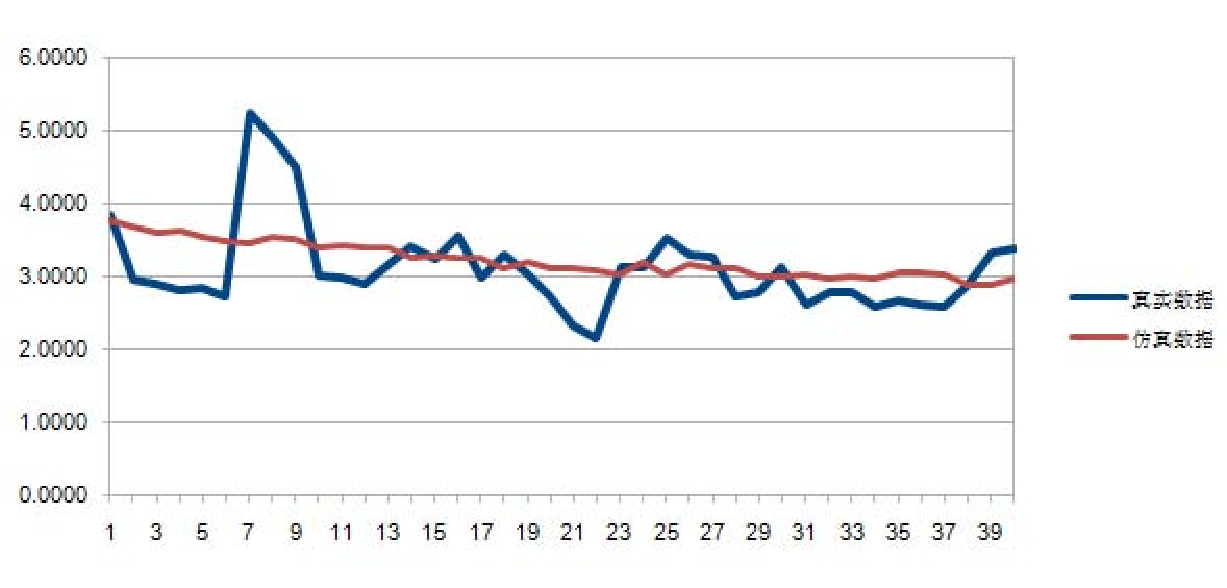
\includegraphics{simu-3.pdf}}
 % GNUPLOT: LaTeX picture
\setlength{\unitlength}{0.240900pt}
\ifx\plotpoint\undefined\newsavebox{\plotpoint}\fi
\begin{picture}(1500,900)(0,0)
\sbox{\plotpoint}{\rule[-0.200pt]{0.400pt}{0.400pt}}%
\put(131.0,82.0){\rule[-0.200pt]{4.818pt}{0.400pt}}
\put(111,82){\makebox(0,0)[r]{ 0}}
\put(1419.0,82.0){\rule[-0.200pt]{4.818pt}{0.400pt}}
\put(131.0,212.0){\rule[-0.200pt]{4.818pt}{0.400pt}}
\put(111,212){\makebox(0,0)[r]{ 1}}
\put(1419.0,212.0){\rule[-0.200pt]{4.818pt}{0.400pt}}
\put(131.0,341.0){\rule[-0.200pt]{4.818pt}{0.400pt}}
\put(111,341){\makebox(0,0)[r]{ 2}}
\put(1419.0,341.0){\rule[-0.200pt]{4.818pt}{0.400pt}}
\put(131.0,471.0){\rule[-0.200pt]{4.818pt}{0.400pt}}
\put(111,471){\makebox(0,0)[r]{ 3}}
\put(1419.0,471.0){\rule[-0.200pt]{4.818pt}{0.400pt}}
\put(131.0,600.0){\rule[-0.200pt]{4.818pt}{0.400pt}}
\put(111,600){\makebox(0,0)[r]{ 4}}
\put(1419.0,600.0){\rule[-0.200pt]{4.818pt}{0.400pt}}
\put(131.0,730.0){\rule[-0.200pt]{4.818pt}{0.400pt}}
\put(111,730){\makebox(0,0)[r]{ 5}}
\put(1419.0,730.0){\rule[-0.200pt]{4.818pt}{0.400pt}}
\put(131.0,859.0){\rule[-0.200pt]{4.818pt}{0.400pt}}
\put(111,859){\makebox(0,0)[r]{ 6}}
\put(1419.0,859.0){\rule[-0.200pt]{4.818pt}{0.400pt}}
\put(131.0,82.0){\rule[-0.200pt]{0.400pt}{4.818pt}}
\put(131,41){\makebox(0,0){ 1}}
\put(131.0,839.0){\rule[-0.200pt]{0.400pt}{4.818pt}}
\put(198.0,82.0){\rule[-0.200pt]{0.400pt}{4.818pt}}
\put(198,41){\makebox(0,0){ 3}}
\put(198.0,839.0){\rule[-0.200pt]{0.400pt}{4.818pt}}
\put(265.0,82.0){\rule[-0.200pt]{0.400pt}{4.818pt}}
\put(265,41){\makebox(0,0){ 5}}
\put(265.0,839.0){\rule[-0.200pt]{0.400pt}{4.818pt}}
\put(332.0,82.0){\rule[-0.200pt]{0.400pt}{4.818pt}}
\put(332,41){\makebox(0,0){ 7}}
\put(332.0,839.0){\rule[-0.200pt]{0.400pt}{4.818pt}}
\put(399.0,82.0){\rule[-0.200pt]{0.400pt}{4.818pt}}
\put(399,41){\makebox(0,0){ 9}}
\put(399.0,839.0){\rule[-0.200pt]{0.400pt}{4.818pt}}
\put(466.0,82.0){\rule[-0.200pt]{0.400pt}{4.818pt}}
\put(466,41){\makebox(0,0){ 11}}
\put(466.0,839.0){\rule[-0.200pt]{0.400pt}{4.818pt}}
\put(533.0,82.0){\rule[-0.200pt]{0.400pt}{4.818pt}}
\put(533,41){\makebox(0,0){ 13}}
\put(533.0,839.0){\rule[-0.200pt]{0.400pt}{4.818pt}}
\put(601.0,82.0){\rule[-0.200pt]{0.400pt}{4.818pt}}
\put(601,41){\makebox(0,0){ 15}}
\put(601.0,839.0){\rule[-0.200pt]{0.400pt}{4.818pt}}
\put(668.0,82.0){\rule[-0.200pt]{0.400pt}{4.818pt}}
\put(668,41){\makebox(0,0){ 17}}
\put(668.0,839.0){\rule[-0.200pt]{0.400pt}{4.818pt}}
\put(735.0,82.0){\rule[-0.200pt]{0.400pt}{4.818pt}}
\put(735,41){\makebox(0,0){ 19}}
\put(735.0,839.0){\rule[-0.200pt]{0.400pt}{4.818pt}}
\put(802.0,82.0){\rule[-0.200pt]{0.400pt}{4.818pt}}
\put(802,41){\makebox(0,0){ 21}}
\put(802.0,839.0){\rule[-0.200pt]{0.400pt}{4.818pt}}
\put(869.0,82.0){\rule[-0.200pt]{0.400pt}{4.818pt}}
\put(869,41){\makebox(0,0){ 23}}
\put(869.0,839.0){\rule[-0.200pt]{0.400pt}{4.818pt}}
\put(936.0,82.0){\rule[-0.200pt]{0.400pt}{4.818pt}}
\put(936,41){\makebox(0,0){ 25}}
\put(936.0,839.0){\rule[-0.200pt]{0.400pt}{4.818pt}}
\put(1003.0,82.0){\rule[-0.200pt]{0.400pt}{4.818pt}}
\put(1003,41){\makebox(0,0){ 27}}
\put(1003.0,839.0){\rule[-0.200pt]{0.400pt}{4.818pt}}
\put(1070.0,82.0){\rule[-0.200pt]{0.400pt}{4.818pt}}
\put(1070,41){\makebox(0,0){ 29}}
\put(1070.0,839.0){\rule[-0.200pt]{0.400pt}{4.818pt}}
\put(1137.0,82.0){\rule[-0.200pt]{0.400pt}{4.818pt}}
\put(1137,41){\makebox(0,0){ 31}}
\put(1137.0,839.0){\rule[-0.200pt]{0.400pt}{4.818pt}}
\put(1204.0,82.0){\rule[-0.200pt]{0.400pt}{4.818pt}}
\put(1204,41){\makebox(0,0){ 33}}
\put(1204.0,839.0){\rule[-0.200pt]{0.400pt}{4.818pt}}
\put(1271.0,82.0){\rule[-0.200pt]{0.400pt}{4.818pt}}
\put(1271,41){\makebox(0,0){ 35}}
\put(1271.0,839.0){\rule[-0.200pt]{0.400pt}{4.818pt}}
\put(1338.0,82.0){\rule[-0.200pt]{0.400pt}{4.818pt}}
\put(1338,41){\makebox(0,0){ 37}}
\put(1338.0,839.0){\rule[-0.200pt]{0.400pt}{4.818pt}}
\put(1405.0,82.0){\rule[-0.200pt]{0.400pt}{4.818pt}}
\put(1405,41){\makebox(0,0){ 39}}
\put(1405.0,839.0){\rule[-0.200pt]{0.400pt}{4.818pt}}
\put(131.0,82.0){\rule[-0.200pt]{0.400pt}{187.179pt}}
\put(131.0,82.0){\rule[-0.200pt]{315.097pt}{0.400pt}}
\put(1439.0,82.0){\rule[-0.200pt]{0.400pt}{187.179pt}}
\put(131.0,859.0){\rule[-0.200pt]{315.097pt}{0.400pt}}
\put(30,470){\makebox(0,0){\rotatebox{90}{用户贡献}}}
\put(785,-10){\makebox(0,0){月度}}
\put(1279,819){\makebox(0,0)[r]{仿真数据}}
\put(1299.0,819.0){\rule[-0.200pt]{24.090pt}{0.400pt}}
\put(1439,547){\usebox{\plotpoint}}
\multiput(1424.47,545.94)(-4.868,-0.468){5}{\rule{3.500pt}{0.113pt}}
\multiput(1431.74,546.17)(-26.736,-4.000){2}{\rule{1.750pt}{0.400pt}}
\multiput(1393.63,541.93)(-3.604,-0.477){7}{\rule{2.740pt}{0.115pt}}
\multiput(1399.31,542.17)(-27.313,-5.000){2}{\rule{1.370pt}{0.400pt}}
\multiput(1357.47,536.94)(-4.868,-0.468){5}{\rule{3.500pt}{0.113pt}}
\multiput(1364.74,537.17)(-26.736,-4.000){2}{\rule{1.750pt}{0.400pt}}
\multiput(1323.89,532.94)(-4.722,-0.468){5}{\rule{3.400pt}{0.113pt}}
\multiput(1330.94,533.17)(-25.943,-4.000){2}{\rule{1.700pt}{0.400pt}}
\multiput(1290.47,528.94)(-4.868,-0.468){5}{\rule{3.500pt}{0.113pt}}
\multiput(1297.74,529.17)(-26.736,-4.000){2}{\rule{1.750pt}{0.400pt}}
\multiput(1256.89,524.94)(-4.722,-0.468){5}{\rule{3.400pt}{0.113pt}}
\multiput(1263.94,525.17)(-25.943,-4.000){2}{\rule{1.700pt}{0.400pt}}
\multiput(1218.77,520.95)(-7.383,-0.447){3}{\rule{4.633pt}{0.108pt}}
\multiput(1228.38,521.17)(-24.383,-3.000){2}{\rule{2.317pt}{0.400pt}}
\multiput(1189.89,517.94)(-4.722,-0.468){5}{\rule{3.400pt}{0.113pt}}
\multiput(1196.94,518.17)(-25.943,-4.000){2}{\rule{1.700pt}{0.400pt}}
\multiput(1151.77,513.95)(-7.383,-0.447){3}{\rule{4.633pt}{0.108pt}}
\multiput(1161.38,514.17)(-24.383,-3.000){2}{\rule{2.317pt}{0.400pt}}
\multiput(1122.89,510.94)(-4.722,-0.468){5}{\rule{3.400pt}{0.113pt}}
\multiput(1129.94,511.17)(-25.943,-4.000){2}{\rule{1.700pt}{0.400pt}}
\multiput(1084.77,506.95)(-7.383,-0.447){3}{\rule{4.633pt}{0.108pt}}
\multiput(1094.38,507.17)(-24.383,-3.000){2}{\rule{2.317pt}{0.400pt}}
\multiput(1051.32,503.95)(-7.160,-0.447){3}{\rule{4.500pt}{0.108pt}}
\multiput(1060.66,504.17)(-23.660,-3.000){2}{\rule{2.250pt}{0.400pt}}
\multiput(1017.77,500.95)(-7.383,-0.447){3}{\rule{4.633pt}{0.108pt}}
\multiput(1027.38,501.17)(-24.383,-3.000){2}{\rule{2.317pt}{0.400pt}}
\multiput(983.77,497.95)(-7.383,-0.447){3}{\rule{4.633pt}{0.108pt}}
\multiput(993.38,498.17)(-24.383,-3.000){2}{\rule{2.317pt}{0.400pt}}
\multiput(950.32,494.95)(-7.160,-0.447){3}{\rule{4.500pt}{0.108pt}}
\multiput(959.66,495.17)(-23.660,-3.000){2}{\rule{2.250pt}{0.400pt}}
\multiput(916.77,491.95)(-7.383,-0.447){3}{\rule{4.633pt}{0.108pt}}
\multiput(926.38,492.17)(-24.383,-3.000){2}{\rule{2.317pt}{0.400pt}}
\multiput(883.32,488.95)(-7.160,-0.447){3}{\rule{4.500pt}{0.108pt}}
\multiput(892.66,489.17)(-23.660,-3.000){2}{\rule{2.250pt}{0.400pt}}
\put(835,485.17){\rule{6.900pt}{0.400pt}}
\multiput(854.68,486.17)(-19.679,-2.000){2}{\rule{3.450pt}{0.400pt}}
\multiput(816.32,483.95)(-7.160,-0.447){3}{\rule{4.500pt}{0.108pt}}
\multiput(825.66,484.17)(-23.660,-3.000){2}{\rule{2.250pt}{0.400pt}}
\put(768,480.17){\rule{6.900pt}{0.400pt}}
\multiput(787.68,481.17)(-19.679,-2.000){2}{\rule{3.450pt}{0.400pt}}
\multiput(749.32,478.95)(-7.160,-0.447){3}{\rule{4.500pt}{0.108pt}}
\multiput(758.66,479.17)(-23.660,-3.000){2}{\rule{2.250pt}{0.400pt}}
\put(701,475.17){\rule{6.900pt}{0.400pt}}
\multiput(720.68,476.17)(-19.679,-2.000){2}{\rule{3.450pt}{0.400pt}}
\put(668,473.17){\rule{6.700pt}{0.400pt}}
\multiput(687.09,474.17)(-19.094,-2.000){2}{\rule{3.350pt}{0.400pt}}
\put(634,471.17){\rule{6.900pt}{0.400pt}}
\multiput(653.68,472.17)(-19.679,-2.000){2}{\rule{3.450pt}{0.400pt}}
\put(601,469.17){\rule{6.700pt}{0.400pt}}
\multiput(620.09,470.17)(-19.094,-2.000){2}{\rule{3.350pt}{0.400pt}}
\put(567,467.67){\rule{8.191pt}{0.400pt}}
\multiput(584.00,468.17)(-17.000,-1.000){2}{\rule{4.095pt}{0.400pt}}
\put(533,466.17){\rule{6.900pt}{0.400pt}}
\multiput(552.68,467.17)(-19.679,-2.000){2}{\rule{3.450pt}{0.400pt}}
\put(500,464.17){\rule{6.700pt}{0.400pt}}
\multiput(519.09,465.17)(-19.094,-2.000){2}{\rule{3.350pt}{0.400pt}}
\put(466,462.67){\rule{8.191pt}{0.400pt}}
\multiput(483.00,463.17)(-17.000,-1.000){2}{\rule{4.095pt}{0.400pt}}
\put(433,461.67){\rule{7.950pt}{0.400pt}}
\multiput(449.50,462.17)(-16.500,-1.000){2}{\rule{3.975pt}{0.400pt}}
\put(399,460.17){\rule{6.900pt}{0.400pt}}
\multiput(418.68,461.17)(-19.679,-2.000){2}{\rule{3.450pt}{0.400pt}}
\put(366,458.67){\rule{7.950pt}{0.400pt}}
\multiput(382.50,459.17)(-16.500,-1.000){2}{\rule{3.975pt}{0.400pt}}
\put(332,457.67){\rule{8.191pt}{0.400pt}}
\multiput(349.00,458.17)(-17.000,-1.000){2}{\rule{4.095pt}{0.400pt}}
\put(299,456.67){\rule{7.950pt}{0.400pt}}
\multiput(315.50,457.17)(-16.500,-1.000){2}{\rule{3.975pt}{0.400pt}}
\put(265,455.67){\rule{8.191pt}{0.400pt}}
\multiput(282.00,456.17)(-17.000,-1.000){2}{\rule{4.095pt}{0.400pt}}
\put(198,454.67){\rule{8.191pt}{0.400pt}}
\multiput(215.00,455.17)(-17.000,-1.000){2}{\rule{4.095pt}{0.400pt}}
\put(232.0,456.0){\rule[-0.200pt]{7.950pt}{0.400pt}}
\put(131,453.67){\rule{8.191pt}{0.400pt}}
\multiput(148.00,454.17)(-17.000,-1.000){2}{\rule{4.095pt}{0.400pt}}
\put(165.0,455.0){\rule[-0.200pt]{7.950pt}{0.400pt}}
\put(1279,768){\makebox(0,0)[r]{实际数据}}
\put(1299.0,768.0){\rule[-0.200pt]{24.090pt}{0.400pt}}
\put(1439,581){\usebox{\plotpoint}}
\multiput(1434.55,581.58)(-1.231,0.494){25}{\rule{1.071pt}{0.119pt}}
\multiput(1436.78,580.17)(-31.776,14.000){2}{\rule{0.536pt}{0.400pt}}
\multiput(1396.76,593.93)(-2.476,-0.485){11}{\rule{1.986pt}{0.117pt}}
\multiput(1400.88,594.17)(-28.879,-7.000){2}{\rule{0.993pt}{0.400pt}}
\multiput(1366.88,586.92)(-1.444,-0.492){21}{\rule{1.233pt}{0.119pt}}
\multiput(1369.44,587.17)(-31.440,-12.000){2}{\rule{0.617pt}{0.400pt}}
\multiput(1319.32,576.61)(-7.160,0.447){3}{\rule{4.500pt}{0.108pt}}
\multiput(1328.66,575.17)(-23.660,3.000){2}{\rule{2.250pt}{0.400pt}}
\multiput(1300.55,577.92)(-1.231,-0.494){25}{\rule{1.071pt}{0.119pt}}
\multiput(1302.78,578.17)(-31.776,-14.000){2}{\rule{0.536pt}{0.400pt}}
\multiput(1269.92,565.00)(-0.497,1.035){63}{\rule{0.120pt}{0.924pt}}
\multiput(1270.17,565.00)(-33.000,66.082){2}{\rule{0.400pt}{0.462pt}}
\multiput(1236.92,633.00)(-0.498,0.856){65}{\rule{0.120pt}{0.782pt}}
\multiput(1237.17,633.00)(-34.000,56.376){2}{\rule{0.400pt}{0.391pt}}
\multiput(1201.39,689.92)(-0.661,-0.497){47}{\rule{0.628pt}{0.120pt}}
\multiput(1202.70,690.17)(-31.697,-25.000){2}{\rule{0.314pt}{0.400pt}}
\multiput(1169.92,658.70)(-0.498,-2.089){65}{\rule{0.120pt}{1.759pt}}
\multiput(1170.17,662.35)(-34.000,-137.349){2}{\rule{0.400pt}{0.879pt}}
\multiput(1135.92,522.47)(-0.497,-0.637){63}{\rule{0.120pt}{0.609pt}}
\multiput(1136.17,523.74)(-33.000,-40.736){2}{\rule{0.400pt}{0.305pt}}
\put(1070,481.67){\rule{8.191pt}{0.400pt}}
\multiput(1087.00,482.17)(-17.000,-1.000){2}{\rule{4.095pt}{0.400pt}}
\multiput(1062.74,482.59)(-2.145,0.488){13}{\rule{1.750pt}{0.117pt}}
\multiput(1066.37,481.17)(-29.368,8.000){2}{\rule{0.875pt}{0.400pt}}
\multiput(1035.92,490.00)(-0.498,0.514){65}{\rule{0.120pt}{0.512pt}}
\multiput(1036.17,490.00)(-34.000,33.938){2}{\rule{0.400pt}{0.256pt}}
\multiput(1000.02,523.92)(-0.775,-0.496){41}{\rule{0.718pt}{0.120pt}}
\multiput(1001.51,524.17)(-32.509,-22.000){2}{\rule{0.359pt}{0.400pt}}
\multiput(967.92,503.00)(-0.497,0.621){63}{\rule{0.120pt}{0.597pt}}
\multiput(968.17,503.00)(-33.000,39.761){2}{\rule{0.400pt}{0.298pt}}
\multiput(934.92,539.82)(-0.498,-1.138){65}{\rule{0.120pt}{1.006pt}}
\multiput(935.17,541.91)(-34.000,-74.912){2}{\rule{0.400pt}{0.503pt}}
\multiput(900.92,467.00)(-0.497,0.637){63}{\rule{0.120pt}{0.609pt}}
\multiput(901.17,467.00)(-33.000,40.736){2}{\rule{0.400pt}{0.305pt}}
\multiput(866.82,507.92)(-0.530,-0.497){61}{\rule{0.525pt}{0.120pt}}
\multiput(867.91,508.17)(-32.910,-32.000){2}{\rule{0.263pt}{0.400pt}}
\multiput(833.92,474.52)(-0.497,-0.621){63}{\rule{0.120pt}{0.597pt}}
\multiput(834.17,475.76)(-33.000,-39.761){2}{\rule{0.400pt}{0.298pt}}
\multiput(800.92,433.05)(-0.498,-0.766){65}{\rule{0.120pt}{0.712pt}}
\multiput(801.17,434.52)(-34.000,-50.523){2}{\rule{0.400pt}{0.356pt}}
\multiput(765.20,382.92)(-0.719,-0.496){43}{\rule{0.674pt}{0.120pt}}
\multiput(766.60,383.17)(-31.601,-23.000){2}{\rule{0.337pt}{0.400pt}}
\multiput(733.92,361.00)(-0.498,1.851){65}{\rule{0.120pt}{1.571pt}}
\multiput(734.17,361.00)(-34.000,121.740){2}{\rule{0.400pt}{0.785pt}}
\put(668,486.17){\rule{6.700pt}{0.400pt}}
\multiput(687.09,485.17)(-19.094,2.000){2}{\rule{3.350pt}{0.400pt}}
\multiput(665.41,488.58)(-0.654,0.497){49}{\rule{0.623pt}{0.120pt}}
\multiput(666.71,487.17)(-32.707,26.000){2}{\rule{0.312pt}{0.400pt}}
\multiput(615.32,512.95)(-7.160,-0.447){3}{\rule{4.500pt}{0.108pt}}
\multiput(624.66,513.17)(-23.660,-3.000){2}{\rule{2.250pt}{0.400pt}}
\multiput(589.29,509.93)(-3.716,-0.477){7}{\rule{2.820pt}{0.115pt}}
\multiput(595.15,510.17)(-28.147,-5.000){2}{\rule{1.410pt}{0.400pt}}
\multiput(565.92,503.39)(-0.498,-0.662){65}{\rule{0.120pt}{0.629pt}}
\multiput(566.17,504.69)(-34.000,-43.694){2}{\rule{0.400pt}{0.315pt}}
\multiput(523.45,461.59)(-2.932,0.482){9}{\rule{2.300pt}{0.116pt}}
\multiput(528.23,460.17)(-28.226,6.000){2}{\rule{1.150pt}{0.400pt}}
\multiput(496.76,467.58)(-0.855,0.496){37}{\rule{0.780pt}{0.119pt}}
\multiput(498.38,466.17)(-32.381,20.000){2}{\rule{0.390pt}{0.400pt}}
\multiput(463.56,485.92)(-0.611,-0.497){51}{\rule{0.589pt}{0.120pt}}
\multiput(464.78,486.17)(-31.778,-27.000){2}{\rule{0.294pt}{0.400pt}}
\multiput(429.61,458.92)(-0.900,-0.495){35}{\rule{0.816pt}{0.119pt}}
\multiput(431.31,459.17)(-32.307,-19.000){2}{\rule{0.408pt}{0.400pt}}
\multiput(380.32,441.61)(-7.160,0.447){3}{\rule{4.500pt}{0.108pt}}
\multiput(389.66,440.17)(-23.660,3.000){2}{\rule{2.250pt}{0.400pt}}
\multiput(317.89,442.94)(-4.722,-0.468){5}{\rule{3.400pt}{0.113pt}}
\multiput(324.94,443.17)(-25.943,-4.000){2}{\rule{1.700pt}{0.400pt}}
\multiput(287.29,438.93)(-3.716,-0.477){7}{\rule{2.820pt}{0.115pt}}
\multiput(293.15,439.17)(-28.147,-5.000){2}{\rule{1.410pt}{0.400pt}}
\multiput(261.98,435.58)(-0.789,0.496){39}{\rule{0.729pt}{0.119pt}}
\multiput(263.49,434.17)(-31.488,21.000){2}{\rule{0.364pt}{0.400pt}}
\multiput(212.77,454.95)(-7.383,-0.447){3}{\rule{4.633pt}{0.108pt}}
\multiput(222.38,455.17)(-24.383,-3.000){2}{\rule{2.317pt}{0.400pt}}
\multiput(196.92,453.00)(-0.497,0.912){63}{\rule{0.120pt}{0.827pt}}
\multiput(197.17,453.00)(-33.000,58.283){2}{\rule{0.400pt}{0.414pt}}
\put(332.0,444.0){\rule[-0.200pt]{8.191pt}{0.400pt}}
\put(1439,581){\makebox(0,0){$+$}}
\put(1405,595){\makebox(0,0){$+$}}
\put(1372,588){\makebox(0,0){$+$}}
\put(1338,576){\makebox(0,0){$+$}}
\put(1305,579){\makebox(0,0){$+$}}
\put(1271,565){\makebox(0,0){$+$}}
\put(1238,633){\makebox(0,0){$+$}}
\put(1204,691){\makebox(0,0){$+$}}
\put(1171,666){\makebox(0,0){$+$}}
\put(1137,525){\makebox(0,0){$+$}}
\put(1104,483){\makebox(0,0){$+$}}
\put(1070,482){\makebox(0,0){$+$}}
\put(1037,490){\makebox(0,0){$+$}}
\put(1003,525){\makebox(0,0){$+$}}
\put(969,503){\makebox(0,0){$+$}}
\put(936,544){\makebox(0,0){$+$}}
\put(902,467){\makebox(0,0){$+$}}
\put(869,509){\makebox(0,0){$+$}}
\put(835,477){\makebox(0,0){$+$}}
\put(802,436){\makebox(0,0){$+$}}
\put(768,384){\makebox(0,0){$+$}}
\put(735,361){\makebox(0,0){$+$}}
\put(701,486){\makebox(0,0){$+$}}
\put(668,488){\makebox(0,0){$+$}}
\put(634,514){\makebox(0,0){$+$}}
\put(601,511){\makebox(0,0){$+$}}
\put(567,506){\makebox(0,0){$+$}}
\put(533,461){\makebox(0,0){$+$}}
\put(500,467){\makebox(0,0){$+$}}
\put(466,487){\makebox(0,0){$+$}}
\put(433,460){\makebox(0,0){$+$}}
\put(399,441){\makebox(0,0){$+$}}
\put(366,444){\makebox(0,0){$+$}}
\put(332,444){\makebox(0,0){$+$}}
\put(299,440){\makebox(0,0){$+$}}
\put(265,435){\makebox(0,0){$+$}}
\put(232,456){\makebox(0,0){$+$}}
\put(198,453){\makebox(0,0){$+$}}
\put(165,513){\makebox(0,0){$+$}}
\put(131,513){\makebox(0,0){$+$}}
\put(1349,768){\makebox(0,0){$+$}}
\put(131.0,513.0){\rule[-0.200pt]{8.191pt}{0.400pt}}
\put(131.0,82.0){\rule[-0.200pt]{0.400pt}{187.179pt}}
\put(131.0,82.0){\rule[-0.200pt]{315.097pt}{0.400pt}}
\put(1439.0,82.0){\rule[-0.200pt]{0.400pt}{187.179pt}}
\put(131.0,859.0){\rule[-0.200pt]{315.097pt}{0.400pt}}
\end{picture}
 
  \caption{\small{\textbf{内容贡献者用户仿真结果}}}
  \label{fig:simu3}
\end{figure}

图\ref{fig:simu4}是内容维护者的仿真结果和真实数据图。实际数据显示内容
维护者的月人均贡献很快下滑,随后逐渐平稳,下滑趋势减缓。仿真数据则是一
条对数曲线,除了和个别真实点的数据结果差距很大以外,整体的拟合度很高,
说明模型对于分析内容维护者的行为是有效的。
\begin{figure}[!htb]
  \centering
%  \scalebox{0.65}{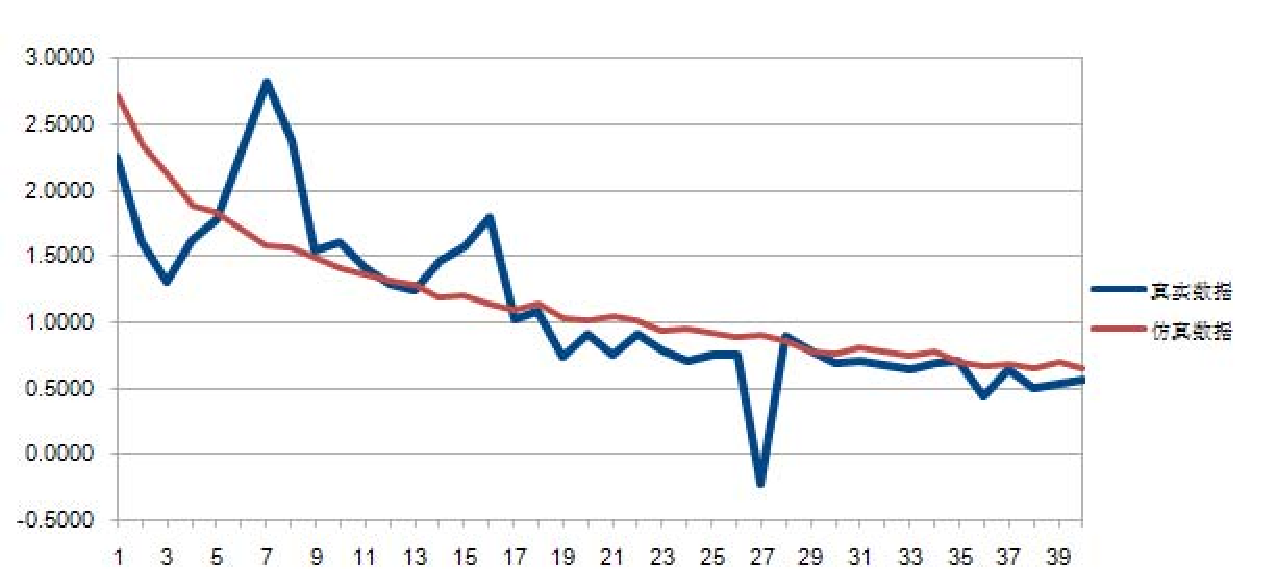
\includegraphics{simu-4.pdf}}
   % GNUPLOT: LaTeX picture
\setlength{\unitlength}{0.240900pt}
\ifx\plotpoint\undefined\newsavebox{\plotpoint}\fi
\begin{picture}(1500,900)(0,0)
\sbox{\plotpoint}{\rule[-0.200pt]{0.400pt}{0.400pt}}%
\put(131.0,82.0){\rule[-0.200pt]{4.818pt}{0.400pt}}
\put(111,82){\makebox(0,0)[r]{-1}}
\put(1419.0,82.0){\rule[-0.200pt]{4.818pt}{0.400pt}}
\put(131.0,237.0){\rule[-0.200pt]{4.818pt}{0.400pt}}
\put(111,237){\makebox(0,0)[r]{ 0}}
\put(1419.0,237.0){\rule[-0.200pt]{4.818pt}{0.400pt}}
\put(131.0,393.0){\rule[-0.200pt]{4.818pt}{0.400pt}}
\put(111,393){\makebox(0,0)[r]{ 1}}
\put(1419.0,393.0){\rule[-0.200pt]{4.818pt}{0.400pt}}
\put(131.0,548.0){\rule[-0.200pt]{4.818pt}{0.400pt}}
\put(111,548){\makebox(0,0)[r]{ 2}}
\put(1419.0,548.0){\rule[-0.200pt]{4.818pt}{0.400pt}}
\put(131.0,704.0){\rule[-0.200pt]{4.818pt}{0.400pt}}
\put(111,704){\makebox(0,0)[r]{ 3}}
\put(1419.0,704.0){\rule[-0.200pt]{4.818pt}{0.400pt}}
\put(131.0,82.0){\rule[-0.200pt]{0.400pt}{4.818pt}}
\put(131,41){\makebox(0,0){ 1}}
\put(131.0,839.0){\rule[-0.200pt]{0.400pt}{4.818pt}}
\put(198.0,82.0){\rule[-0.200pt]{0.400pt}{4.818pt}}
\put(198,41){\makebox(0,0){ 3}}
\put(198.0,839.0){\rule[-0.200pt]{0.400pt}{4.818pt}}
\put(265.0,82.0){\rule[-0.200pt]{0.400pt}{4.818pt}}
\put(265,41){\makebox(0,0){ 5}}
\put(265.0,839.0){\rule[-0.200pt]{0.400pt}{4.818pt}}
\put(332.0,82.0){\rule[-0.200pt]{0.400pt}{4.818pt}}
\put(332,41){\makebox(0,0){ 7}}
\put(332.0,839.0){\rule[-0.200pt]{0.400pt}{4.818pt}}
\put(399.0,82.0){\rule[-0.200pt]{0.400pt}{4.818pt}}
\put(399,41){\makebox(0,0){ 9}}
\put(399.0,839.0){\rule[-0.200pt]{0.400pt}{4.818pt}}
\put(466.0,82.0){\rule[-0.200pt]{0.400pt}{4.818pt}}
\put(466,41){\makebox(0,0){ 11}}
\put(466.0,839.0){\rule[-0.200pt]{0.400pt}{4.818pt}}
\put(533.0,82.0){\rule[-0.200pt]{0.400pt}{4.818pt}}
\put(533,41){\makebox(0,0){ 13}}
\put(533.0,839.0){\rule[-0.200pt]{0.400pt}{4.818pt}}
\put(601.0,82.0){\rule[-0.200pt]{0.400pt}{4.818pt}}
\put(601,41){\makebox(0,0){ 15}}
\put(601.0,839.0){\rule[-0.200pt]{0.400pt}{4.818pt}}
\put(668.0,82.0){\rule[-0.200pt]{0.400pt}{4.818pt}}
\put(668,41){\makebox(0,0){ 17}}
\put(668.0,839.0){\rule[-0.200pt]{0.400pt}{4.818pt}}
\put(735.0,82.0){\rule[-0.200pt]{0.400pt}{4.818pt}}
\put(735,41){\makebox(0,0){ 19}}
\put(735.0,839.0){\rule[-0.200pt]{0.400pt}{4.818pt}}
\put(802.0,82.0){\rule[-0.200pt]{0.400pt}{4.818pt}}
\put(802,41){\makebox(0,0){ 21}}
\put(802.0,839.0){\rule[-0.200pt]{0.400pt}{4.818pt}}
\put(869.0,82.0){\rule[-0.200pt]{0.400pt}{4.818pt}}
\put(869,41){\makebox(0,0){ 23}}
\put(869.0,839.0){\rule[-0.200pt]{0.400pt}{4.818pt}}
\put(936.0,82.0){\rule[-0.200pt]{0.400pt}{4.818pt}}
\put(936,41){\makebox(0,0){ 25}}
\put(936.0,839.0){\rule[-0.200pt]{0.400pt}{4.818pt}}
\put(1003.0,82.0){\rule[-0.200pt]{0.400pt}{4.818pt}}
\put(1003,41){\makebox(0,0){ 27}}
\put(1003.0,839.0){\rule[-0.200pt]{0.400pt}{4.818pt}}
\put(1070.0,82.0){\rule[-0.200pt]{0.400pt}{4.818pt}}
\put(1070,41){\makebox(0,0){ 29}}
\put(1070.0,839.0){\rule[-0.200pt]{0.400pt}{4.818pt}}
\put(1137.0,82.0){\rule[-0.200pt]{0.400pt}{4.818pt}}
\put(1137,41){\makebox(0,0){ 31}}
\put(1137.0,839.0){\rule[-0.200pt]{0.400pt}{4.818pt}}
\put(1204.0,82.0){\rule[-0.200pt]{0.400pt}{4.818pt}}
\put(1204,41){\makebox(0,0){ 33}}
\put(1204.0,839.0){\rule[-0.200pt]{0.400pt}{4.818pt}}
\put(1271.0,82.0){\rule[-0.200pt]{0.400pt}{4.818pt}}
\put(1271,41){\makebox(0,0){ 35}}
\put(1271.0,839.0){\rule[-0.200pt]{0.400pt}{4.818pt}}
\put(1338.0,82.0){\rule[-0.200pt]{0.400pt}{4.818pt}}
\put(1338,41){\makebox(0,0){ 37}}
\put(1338.0,839.0){\rule[-0.200pt]{0.400pt}{4.818pt}}
\put(1405.0,82.0){\rule[-0.200pt]{0.400pt}{4.818pt}}
\put(1405,41){\makebox(0,0){ 39}}
\put(1405.0,839.0){\rule[-0.200pt]{0.400pt}{4.818pt}}
\put(131.0,82.0){\rule[-0.200pt]{0.400pt}{187.179pt}}
\put(131.0,82.0){\rule[-0.200pt]{315.097pt}{0.400pt}}
\put(1439.0,82.0){\rule[-0.200pt]{0.400pt}{187.179pt}}
\put(131.0,859.0){\rule[-0.200pt]{315.097pt}{0.400pt}}
\put(30,470){\makebox(0,0){\rotatebox{90}{用户贡献}}}
\put(1279,819){\makebox(0,0)[r]{仿真数据}}
\put(785,-10){\makebox(0,0){月度}}
\put(1299.0,819.0){\rule[-0.200pt]{24.090pt}{0.400pt}}
\put(131,646){\usebox{\plotpoint}}
\multiput(131.58,643.05)(0.498,-0.766){65}{\rule{0.120pt}{0.712pt}}
\multiput(130.17,644.52)(34.000,-50.523){2}{\rule{0.400pt}{0.356pt}}
\multiput(165.00,592.92)(0.549,-0.497){57}{\rule{0.540pt}{0.120pt}}
\multiput(165.00,593.17)(31.879,-30.000){2}{\rule{0.270pt}{0.400pt}}
\multiput(198.00,562.92)(0.607,-0.497){53}{\rule{0.586pt}{0.120pt}}
\multiput(198.00,563.17)(32.784,-28.000){2}{\rule{0.293pt}{0.400pt}}
\multiput(232.00,534.92)(0.979,-0.495){31}{\rule{0.876pt}{0.119pt}}
\multiput(232.00,535.17)(31.181,-17.000){2}{\rule{0.438pt}{0.400pt}}
\multiput(265.00,517.92)(1.231,-0.494){25}{\rule{1.071pt}{0.119pt}}
\multiput(265.00,518.17)(31.776,-14.000){2}{\rule{0.536pt}{0.400pt}}
\multiput(299.00,503.92)(0.874,-0.495){35}{\rule{0.795pt}{0.119pt}}
\multiput(299.00,504.17)(31.350,-19.000){2}{\rule{0.397pt}{0.400pt}}
\multiput(332.00,484.93)(2.211,-0.488){13}{\rule{1.800pt}{0.117pt}}
\multiput(332.00,485.17)(30.264,-8.000){2}{\rule{0.900pt}{0.400pt}}
\multiput(366.00,476.93)(3.604,-0.477){7}{\rule{2.740pt}{0.115pt}}
\multiput(366.00,477.17)(27.313,-5.000){2}{\rule{1.370pt}{0.400pt}}
\multiput(399.00,471.92)(1.329,-0.493){23}{\rule{1.146pt}{0.119pt}}
\multiput(399.00,472.17)(31.621,-13.000){2}{\rule{0.573pt}{0.400pt}}
\multiput(433.00,458.92)(1.041,-0.494){29}{\rule{0.925pt}{0.119pt}}
\multiput(433.00,459.17)(31.080,-16.000){2}{\rule{0.463pt}{0.400pt}}
\put(466,443.67){\rule{8.191pt}{0.400pt}}
\multiput(466.00,443.17)(17.000,1.000){2}{\rule{4.095pt}{0.400pt}}
\multiput(500.00,443.93)(3.604,-0.477){7}{\rule{2.740pt}{0.115pt}}
\multiput(500.00,444.17)(27.313,-5.000){2}{\rule{1.370pt}{0.400pt}}
\multiput(533.00,438.93)(2.552,-0.485){11}{\rule{2.043pt}{0.117pt}}
\multiput(533.00,439.17)(29.760,-7.000){2}{\rule{1.021pt}{0.400pt}}
\multiput(567.00,431.93)(3.716,-0.477){7}{\rule{2.820pt}{0.115pt}}
\multiput(567.00,432.17)(28.147,-5.000){2}{\rule{1.410pt}{0.400pt}}
\multiput(601.00,426.93)(3.604,-0.477){7}{\rule{2.740pt}{0.115pt}}
\multiput(601.00,427.17)(27.313,-5.000){2}{\rule{1.370pt}{0.400pt}}
\multiput(634.00,421.93)(3.716,-0.477){7}{\rule{2.820pt}{0.115pt}}
\multiput(634.00,422.17)(28.147,-5.000){2}{\rule{1.410pt}{0.400pt}}
\multiput(668.00,416.93)(1.893,-0.489){15}{\rule{1.567pt}{0.118pt}}
\multiput(668.00,417.17)(29.748,-9.000){2}{\rule{0.783pt}{0.400pt}}
\multiput(701.00,407.94)(4.868,-0.468){5}{\rule{3.500pt}{0.113pt}}
\multiput(701.00,408.17)(26.736,-4.000){2}{\rule{1.750pt}{0.400pt}}
\multiput(735.00,403.93)(2.932,-0.482){9}{\rule{2.300pt}{0.116pt}}
\multiput(735.00,404.17)(28.226,-6.000){2}{\rule{1.150pt}{0.400pt}}
\multiput(768.00,397.93)(2.552,-0.485){11}{\rule{2.043pt}{0.117pt}}
\multiput(768.00,398.17)(29.760,-7.000){2}{\rule{1.021pt}{0.400pt}}
\put(802,391.67){\rule{7.950pt}{0.400pt}}
\multiput(802.00,391.17)(16.500,1.000){2}{\rule{3.975pt}{0.400pt}}
\multiput(835.00,391.93)(2.211,-0.488){13}{\rule{1.800pt}{0.117pt}}
\multiput(835.00,392.17)(30.264,-8.000){2}{\rule{0.900pt}{0.400pt}}
\multiput(869.00,383.93)(2.932,-0.482){9}{\rule{2.300pt}{0.116pt}}
\multiput(869.00,384.17)(28.226,-6.000){2}{\rule{1.150pt}{0.400pt}}
\multiput(902.00,377.95)(7.383,-0.447){3}{\rule{4.633pt}{0.108pt}}
\multiput(902.00,378.17)(24.383,-3.000){2}{\rule{2.317pt}{0.400pt}}
\put(936,376.17){\rule{6.700pt}{0.400pt}}
\multiput(936.00,375.17)(19.094,2.000){2}{\rule{3.350pt}{0.400pt}}
\multiput(969.00,376.94)(4.868,-0.468){5}{\rule{3.500pt}{0.113pt}}
\multiput(969.00,377.17)(26.736,-4.000){2}{\rule{1.750pt}{0.400pt}}
\multiput(1003.00,372.93)(2.211,-0.488){13}{\rule{1.800pt}{0.117pt}}
\multiput(1003.00,373.17)(30.264,-8.000){2}{\rule{0.900pt}{0.400pt}}
\multiput(1037.00,364.93)(2.476,-0.485){11}{\rule{1.986pt}{0.117pt}}
\multiput(1037.00,365.17)(28.879,-7.000){2}{\rule{0.993pt}{0.400pt}}
\put(1070,357.67){\rule{8.191pt}{0.400pt}}
\multiput(1070.00,358.17)(17.000,-1.000){2}{\rule{4.095pt}{0.400pt}}
\multiput(1104.00,356.94)(4.722,-0.468){5}{\rule{3.400pt}{0.113pt}}
\multiput(1104.00,357.17)(25.943,-4.000){2}{\rule{1.700pt}{0.400pt}}
\multiput(1137.00,352.94)(4.868,-0.468){5}{\rule{3.500pt}{0.113pt}}
\multiput(1137.00,353.17)(26.736,-4.000){2}{\rule{1.750pt}{0.400pt}}
\put(1171,348.67){\rule{7.950pt}{0.400pt}}
\multiput(1171.00,349.17)(16.500,-1.000){2}{\rule{3.975pt}{0.400pt}}
\put(1238,347.17){\rule{6.700pt}{0.400pt}}
\multiput(1238.00,348.17)(19.094,-2.000){2}{\rule{3.350pt}{0.400pt}}
\put(1271,345.67){\rule{8.191pt}{0.400pt}}
\multiput(1271.00,346.17)(17.000,-1.000){2}{\rule{4.095pt}{0.400pt}}
\put(1305,345.67){\rule{7.950pt}{0.400pt}}
\multiput(1305.00,345.17)(16.500,1.000){2}{\rule{3.975pt}{0.400pt}}
\put(1204.0,349.0){\rule[-0.200pt]{8.191pt}{0.400pt}}
\multiput(1372.00,345.93)(2.476,-0.485){11}{\rule{1.986pt}{0.117pt}}
\multiput(1372.00,346.17)(28.879,-7.000){2}{\rule{0.993pt}{0.400pt}}
\put(1405,338.17){\rule{6.900pt}{0.400pt}}
\multiput(1405.00,339.17)(19.679,-2.000){2}{\rule{3.450pt}{0.400pt}}
\put(1338.0,347.0){\rule[-0.200pt]{8.191pt}{0.400pt}}
\put(1279,768){\makebox(0,0)[r]{实际数据}}
\put(1299.0,768.0){\rule[-0.200pt]{24.090pt}{0.400pt}}
\put(131,587){\usebox{\plotpoint}}
\multiput(131.58,581.75)(0.498,-1.465){65}{\rule{0.120pt}{1.265pt}}
\multiput(130.17,584.38)(34.000,-96.375){2}{\rule{0.400pt}{0.632pt}}
\multiput(165.58,485.12)(0.497,-0.744){63}{\rule{0.120pt}{0.694pt}}
\multiput(164.17,486.56)(33.000,-47.560){2}{\rule{0.400pt}{0.347pt}}
\multiput(198.58,439.00)(0.498,0.751){65}{\rule{0.120pt}{0.700pt}}
\multiput(197.17,439.00)(34.000,49.547){2}{\rule{0.400pt}{0.350pt}}
\multiput(232.00,490.58)(0.719,0.496){43}{\rule{0.674pt}{0.120pt}}
\multiput(232.00,489.17)(31.601,23.000){2}{\rule{0.337pt}{0.400pt}}
\multiput(265.58,513.00)(0.498,1.197){65}{\rule{0.120pt}{1.053pt}}
\multiput(264.17,513.00)(34.000,78.815){2}{\rule{0.400pt}{0.526pt}}
\multiput(299.58,594.00)(0.497,1.265){63}{\rule{0.120pt}{1.106pt}}
\multiput(298.17,594.00)(33.000,80.704){2}{\rule{0.400pt}{0.553pt}}
\multiput(332.58,673.17)(0.498,-1.034){65}{\rule{0.120pt}{0.924pt}}
\multiput(331.17,675.08)(34.000,-68.083){2}{\rule{0.400pt}{0.462pt}}
\multiput(366.58,600.09)(0.497,-1.969){63}{\rule{0.120pt}{1.664pt}}
\multiput(365.17,603.55)(33.000,-125.547){2}{\rule{0.400pt}{0.832pt}}
\multiput(399.00,478.59)(1.951,0.489){15}{\rule{1.611pt}{0.118pt}}
\multiput(399.00,477.17)(30.656,9.000){2}{\rule{0.806pt}{0.400pt}}
\multiput(433.00,485.92)(0.549,-0.497){57}{\rule{0.540pt}{0.120pt}}
\multiput(433.00,486.17)(31.879,-30.000){2}{\rule{0.270pt}{0.400pt}}
\multiput(466.00,455.92)(0.855,-0.496){37}{\rule{0.780pt}{0.119pt}}
\multiput(466.00,456.17)(32.381,-20.000){2}{\rule{0.390pt}{0.400pt}}
\multiput(500.00,435.93)(2.476,-0.485){11}{\rule{1.986pt}{0.117pt}}
\multiput(500.00,436.17)(28.879,-7.000){2}{\rule{0.993pt}{0.400pt}}
\multiput(533.58,430.00)(0.498,0.514){65}{\rule{0.120pt}{0.512pt}}
\multiput(532.17,430.00)(34.000,33.938){2}{\rule{0.400pt}{0.256pt}}
\multiput(567.00,465.58)(1.009,0.495){31}{\rule{0.900pt}{0.119pt}}
\multiput(567.00,464.17)(32.132,17.000){2}{\rule{0.450pt}{0.400pt}}
\multiput(601.58,482.00)(0.497,0.529){63}{\rule{0.120pt}{0.524pt}}
\multiput(600.17,482.00)(33.000,33.912){2}{\rule{0.400pt}{0.262pt}}
\multiput(634.58,510.68)(0.498,-1.792){65}{\rule{0.120pt}{1.524pt}}
\multiput(633.17,513.84)(34.000,-117.838){2}{\rule{0.400pt}{0.762pt}}
\multiput(668.00,396.58)(1.694,0.491){17}{\rule{1.420pt}{0.118pt}}
\multiput(668.00,395.17)(30.053,10.000){2}{\rule{0.710pt}{0.400pt}}
\multiput(701.58,402.95)(0.498,-0.796){65}{\rule{0.120pt}{0.735pt}}
\multiput(700.17,404.47)(34.000,-52.474){2}{\rule{0.400pt}{0.368pt}}
\multiput(735.00,352.58)(0.635,0.497){49}{\rule{0.608pt}{0.120pt}}
\multiput(735.00,351.17)(31.739,26.000){2}{\rule{0.304pt}{0.400pt}}
\multiput(768.00,376.92)(0.775,-0.496){41}{\rule{0.718pt}{0.120pt}}
\multiput(768.00,377.17)(32.509,-22.000){2}{\rule{0.359pt}{0.400pt}}
\multiput(802.00,356.58)(0.752,0.496){41}{\rule{0.700pt}{0.120pt}}
\multiput(802.00,355.17)(31.547,22.000){2}{\rule{0.350pt}{0.400pt}}
\multiput(835.00,376.92)(0.952,-0.495){33}{\rule{0.856pt}{0.119pt}}
\multiput(835.00,377.17)(32.224,-18.000){2}{\rule{0.428pt}{0.400pt}}
\multiput(869.00,358.92)(1.401,-0.492){21}{\rule{1.200pt}{0.119pt}}
\multiput(869.00,359.17)(30.509,-12.000){2}{\rule{0.600pt}{0.400pt}}
\multiput(902.00,348.59)(2.552,0.485){11}{\rule{2.043pt}{0.117pt}}
\multiput(902.00,347.17)(29.760,7.000){2}{\rule{1.021pt}{0.400pt}}
\put(936,354.67){\rule{7.950pt}{0.400pt}}
\multiput(936.00,354.17)(16.500,1.000){2}{\rule{3.975pt}{0.400pt}}
\multiput(969.58,348.11)(0.498,-2.267){65}{\rule{0.120pt}{1.900pt}}
\multiput(968.17,352.06)(34.000,-149.056){2}{\rule{0.400pt}{0.950pt}}
\multiput(1003.58,203.00)(0.498,2.579){65}{\rule{0.120pt}{2.147pt}}
\multiput(1002.17,203.00)(34.000,169.544){2}{\rule{0.400pt}{1.074pt}}
\multiput(1037.00,375.92)(0.923,-0.495){33}{\rule{0.833pt}{0.119pt}}
\multiput(1037.00,376.17)(31.270,-18.000){2}{\rule{0.417pt}{0.400pt}}
\multiput(1070.00,357.92)(1.329,-0.493){23}{\rule{1.146pt}{0.119pt}}
\multiput(1070.00,358.17)(31.621,-13.000){2}{\rule{0.573pt}{0.400pt}}
\put(1104,345.67){\rule{7.950pt}{0.400pt}}
\multiput(1104.00,345.17)(16.500,1.000){2}{\rule{3.975pt}{0.400pt}}
\multiput(1137.00,345.94)(4.868,-0.468){5}{\rule{3.500pt}{0.113pt}}
\multiput(1137.00,346.17)(26.736,-4.000){2}{\rule{1.750pt}{0.400pt}}
\multiput(1171.00,341.93)(3.604,-0.477){7}{\rule{2.740pt}{0.115pt}}
\multiput(1171.00,342.17)(27.313,-5.000){2}{\rule{1.370pt}{0.400pt}}
\multiput(1204.00,338.59)(3.022,0.482){9}{\rule{2.367pt}{0.116pt}}
\multiput(1204.00,337.17)(29.088,6.000){2}{\rule{1.183pt}{0.400pt}}
\multiput(1238.00,344.61)(7.160,0.447){3}{\rule{4.500pt}{0.108pt}}
\multiput(1238.00,343.17)(23.660,3.000){2}{\rule{2.250pt}{0.400pt}}
\multiput(1271.58,344.63)(0.498,-0.588){65}{\rule{0.120pt}{0.571pt}}
\multiput(1270.17,345.82)(34.000,-38.816){2}{\rule{0.400pt}{0.285pt}}
\multiput(1305.00,307.58)(0.531,0.497){59}{\rule{0.526pt}{0.120pt}}
\multiput(1305.00,306.17)(31.909,31.000){2}{\rule{0.263pt}{0.400pt}}
\multiput(1338.00,336.92)(0.741,-0.496){43}{\rule{0.691pt}{0.120pt}}
\multiput(1338.00,337.17)(32.565,-23.000){2}{\rule{0.346pt}{0.400pt}}
\multiput(1372.00,315.59)(2.932,0.482){9}{\rule{2.300pt}{0.116pt}}
\multiput(1372.00,314.17)(28.226,6.000){2}{\rule{1.150pt}{0.400pt}}
\multiput(1405.00,321.60)(4.868,0.468){5}{\rule{3.500pt}{0.113pt}}
\multiput(1405.00,320.17)(26.736,4.000){2}{\rule{1.750pt}{0.400pt}}
\put(131,587){\makebox(0,0){$+$}}
\put(165,488){\makebox(0,0){$+$}}
\put(198,439){\makebox(0,0){$+$}}
\put(232,490){\makebox(0,0){$+$}}
\put(265,513){\makebox(0,0){$+$}}
\put(299,594){\makebox(0,0){$+$}}
\put(332,677){\makebox(0,0){$+$}}
\put(366,607){\makebox(0,0){$+$}}
\put(399,478){\makebox(0,0){$+$}}
\put(433,487){\makebox(0,0){$+$}}
\put(466,457){\makebox(0,0){$+$}}
\put(500,437){\makebox(0,0){$+$}}
\put(533,430){\makebox(0,0){$+$}}
\put(567,465){\makebox(0,0){$+$}}
\put(601,482){\makebox(0,0){$+$}}
\put(634,517){\makebox(0,0){$+$}}
\put(668,396){\makebox(0,0){$+$}}
\put(701,406){\makebox(0,0){$+$}}
\put(735,352){\makebox(0,0){$+$}}
\put(768,378){\makebox(0,0){$+$}}
\put(802,356){\makebox(0,0){$+$}}
\put(835,378){\makebox(0,0){$+$}}
\put(869,360){\makebox(0,0){$+$}}
\put(902,348){\makebox(0,0){$+$}}
\put(936,355){\makebox(0,0){$+$}}
\put(969,356){\makebox(0,0){$+$}}
\put(1003,203){\makebox(0,0){$+$}}
\put(1037,377){\makebox(0,0){$+$}}
\put(1070,359){\makebox(0,0){$+$}}
\put(1104,346){\makebox(0,0){$+$}}
\put(1137,347){\makebox(0,0){$+$}}
\put(1171,343){\makebox(0,0){$+$}}
\put(1204,338){\makebox(0,0){$+$}}
\put(1238,344){\makebox(0,0){$+$}}
\put(1271,347){\makebox(0,0){$+$}}
\put(1305,307){\makebox(0,0){$+$}}
\put(1338,338){\makebox(0,0){$+$}}
\put(1372,315){\makebox(0,0){$+$}}
\put(1405,321){\makebox(0,0){$+$}}
\put(1439,325){\makebox(0,0){$+$}}
\put(1349,768){\makebox(0,0){$+$}}
\put(131.0,82.0){\rule[-0.200pt]{0.400pt}{187.179pt}}
\put(131.0,82.0){\rule[-0.200pt]{315.097pt}{0.400pt}}
\put(1439.0,82.0){\rule[-0.200pt]{0.400pt}{187.179pt}}
\put(131.0,859.0){\rule[-0.200pt]{315.097pt}{0.400pt}}
\end{picture}
 
  \caption{\small{\textbf{内容维护者用户仿真结果}}}
  \label{fig:simu4}
\end{figure}

图\ref{fig:simu5}是边缘用户的仿真结果和真实数据图。边缘用户的月人均贡
献值是所有用户类型中最为特殊的:呈加速下滑趋势。模型仿真结果也显示月人均贡献是一条近
似于指数函数的曲线。虽然真实数据的波动水平比较大,但是模型的拟合结果仍
然反映了真实系统的变动趋势。
\begin{figure}[!htb]
  \centering
%  \scalebox{0.65}{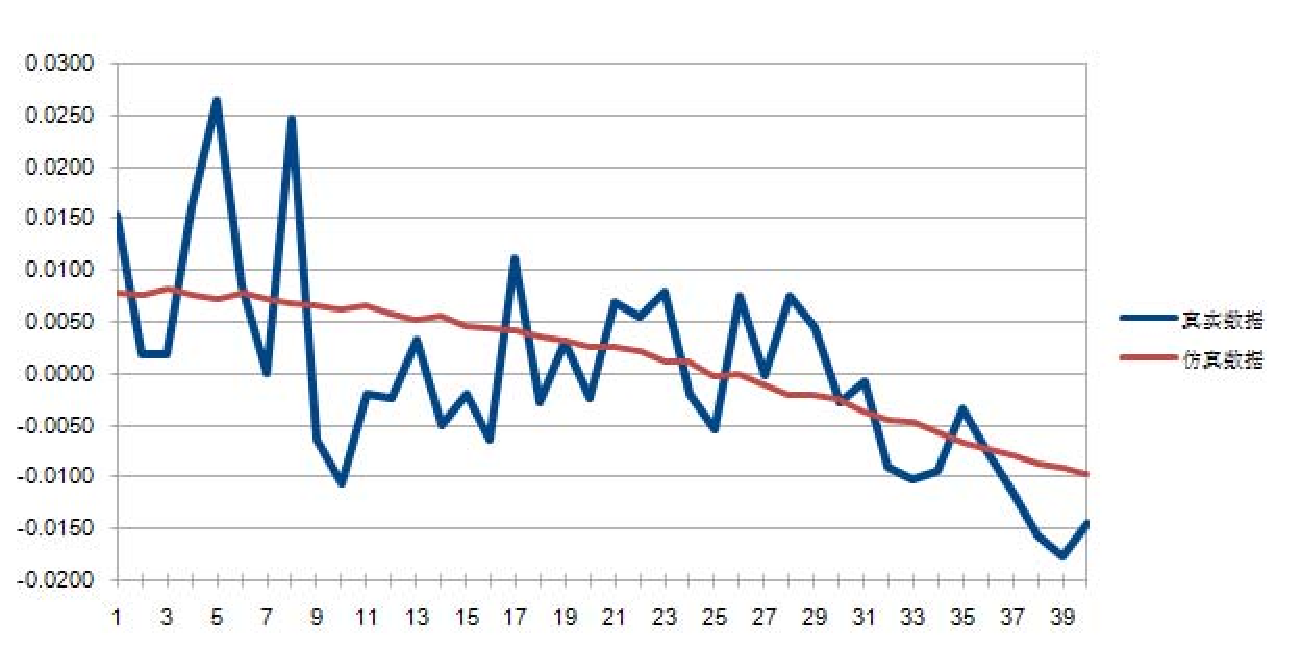
\includegraphics{simu-5.pdf}}
% GNUPLOT: LaTeX picture
\setlength{\unitlength}{0.240900pt}
\ifx\plotpoint\undefined\newsavebox{\plotpoint}\fi
\begin{picture}(1500,900)(0,0)
\sbox{\plotpoint}{\rule[-0.200pt]{0.400pt}{0.400pt}}%
\put(211.0,82.0){\rule[-0.200pt]{4.818pt}{0.400pt}}
\put(191,82){\makebox(0,0)[r]{-0.02}}
\put(1419.0,82.0){\rule[-0.200pt]{4.818pt}{0.400pt}}
\put(211.0,143.0){\rule[-0.200pt]{4.818pt}{0.400pt}}
\put(191,143){\makebox(0,0)[r]{-0.015}}
\put(1419.0,143.0){\rule[-0.200pt]{4.818pt}{0.400pt}}
\put(211.0,203.0){\rule[-0.200pt]{4.818pt}{0.400pt}}
\put(191,203){\makebox(0,0)[r]{-0.01}}
\put(1419.0,203.0){\rule[-0.200pt]{4.818pt}{0.400pt}}
\put(211.0,264.0){\rule[-0.200pt]{4.818pt}{0.400pt}}
\put(191,264){\makebox(0,0)[r]{-0.005}}
\put(1419.0,264.0){\rule[-0.200pt]{4.818pt}{0.400pt}}
\put(211.0,325.0){\rule[-0.200pt]{4.818pt}{0.400pt}}
\put(191,325){\makebox(0,0)[r]{ 0}}
\put(1419.0,325.0){\rule[-0.200pt]{4.818pt}{0.400pt}}
\put(211.0,386.0){\rule[-0.200pt]{4.818pt}{0.400pt}}
\put(191,386){\makebox(0,0)[r]{ 0.005}}
\put(1419.0,386.0){\rule[-0.200pt]{4.818pt}{0.400pt}}
\put(211.0,446.0){\rule[-0.200pt]{4.818pt}{0.400pt}}
\put(191,446){\makebox(0,0)[r]{ 0.01}}
\put(1419.0,446.0){\rule[-0.200pt]{4.818pt}{0.400pt}}
\put(211.0,507.0){\rule[-0.200pt]{4.818pt}{0.400pt}}
\put(191,507){\makebox(0,0)[r]{ 0.015}}
\put(1419.0,507.0){\rule[-0.200pt]{4.818pt}{0.400pt}}
\put(211.0,568.0){\rule[-0.200pt]{4.818pt}{0.400pt}}
\put(191,568){\makebox(0,0)[r]{ 0.02}}
\put(1419.0,568.0){\rule[-0.200pt]{4.818pt}{0.400pt}}
\put(211.0,628.0){\rule[-0.200pt]{4.818pt}{0.400pt}}
\put(191,628){\makebox(0,0)[r]{ 0.025}}
\put(1419.0,628.0){\rule[-0.200pt]{4.818pt}{0.400pt}}
\put(211.0,689.0){\rule[-0.200pt]{4.818pt}{0.400pt}}
\put(191,689){\makebox(0,0)[r]{ 0.03}}
\put(1419.0,689.0){\rule[-0.200pt]{4.818pt}{0.400pt}}
\put(211.0,82.0){\rule[-0.200pt]{0.400pt}{4.818pt}}
\put(211,41){\makebox(0,0){ 1}}
\put(211.0,839.0){\rule[-0.200pt]{0.400pt}{4.818pt}}
\put(274.0,82.0){\rule[-0.200pt]{0.400pt}{4.818pt}}
\put(274,41){\makebox(0,0){ 3}}
\put(274.0,839.0){\rule[-0.200pt]{0.400pt}{4.818pt}}
\put(337.0,82.0){\rule[-0.200pt]{0.400pt}{4.818pt}}
\put(337,41){\makebox(0,0){ 5}}
\put(337.0,839.0){\rule[-0.200pt]{0.400pt}{4.818pt}}
\put(400.0,82.0){\rule[-0.200pt]{0.400pt}{4.818pt}}
\put(400,41){\makebox(0,0){ 7}}
\put(400.0,839.0){\rule[-0.200pt]{0.400pt}{4.818pt}}
\put(463.0,82.0){\rule[-0.200pt]{0.400pt}{4.818pt}}
\put(463,41){\makebox(0,0){ 9}}
\put(463.0,839.0){\rule[-0.200pt]{0.400pt}{4.818pt}}
\put(526.0,82.0){\rule[-0.200pt]{0.400pt}{4.818pt}}
\put(526,41){\makebox(0,0){ 11}}
\put(526.0,839.0){\rule[-0.200pt]{0.400pt}{4.818pt}}
\put(589.0,82.0){\rule[-0.200pt]{0.400pt}{4.818pt}}
\put(589,41){\makebox(0,0){ 13}}
\put(589.0,839.0){\rule[-0.200pt]{0.400pt}{4.818pt}}
\put(652.0,82.0){\rule[-0.200pt]{0.400pt}{4.818pt}}
\put(652,41){\makebox(0,0){ 15}}
\put(652.0,839.0){\rule[-0.200pt]{0.400pt}{4.818pt}}
\put(715.0,82.0){\rule[-0.200pt]{0.400pt}{4.818pt}}
\put(715,41){\makebox(0,0){ 17}}
\put(715.0,839.0){\rule[-0.200pt]{0.400pt}{4.818pt}}
\put(778.0,82.0){\rule[-0.200pt]{0.400pt}{4.818pt}}
\put(778,41){\makebox(0,0){ 19}}
\put(778.0,839.0){\rule[-0.200pt]{0.400pt}{4.818pt}}
\put(841.0,82.0){\rule[-0.200pt]{0.400pt}{4.818pt}}
\put(841,41){\makebox(0,0){ 21}}
\put(841.0,839.0){\rule[-0.200pt]{0.400pt}{4.818pt}}
\put(904.0,82.0){\rule[-0.200pt]{0.400pt}{4.818pt}}
\put(904,41){\makebox(0,0){ 23}}
\put(904.0,839.0){\rule[-0.200pt]{0.400pt}{4.818pt}}
\put(967.0,82.0){\rule[-0.200pt]{0.400pt}{4.818pt}}
\put(967,41){\makebox(0,0){ 25}}
\put(967.0,839.0){\rule[-0.200pt]{0.400pt}{4.818pt}}
\put(1030.0,82.0){\rule[-0.200pt]{0.400pt}{4.818pt}}
\put(1030,41){\makebox(0,0){ 27}}
\put(1030.0,839.0){\rule[-0.200pt]{0.400pt}{4.818pt}}
\put(1093.0,82.0){\rule[-0.200pt]{0.400pt}{4.818pt}}
\put(1093,41){\makebox(0,0){ 29}}
\put(1093.0,839.0){\rule[-0.200pt]{0.400pt}{4.818pt}}
\put(1156.0,82.0){\rule[-0.200pt]{0.400pt}{4.818pt}}
\put(1156,41){\makebox(0,0){ 31}}
\put(1156.0,839.0){\rule[-0.200pt]{0.400pt}{4.818pt}}
\put(1219.0,82.0){\rule[-0.200pt]{0.400pt}{4.818pt}}
\put(1219,41){\makebox(0,0){ 33}}
\put(1219.0,839.0){\rule[-0.200pt]{0.400pt}{4.818pt}}
\put(1282.0,82.0){\rule[-0.200pt]{0.400pt}{4.818pt}}
\put(1282,41){\makebox(0,0){ 35}}
\put(1282.0,839.0){\rule[-0.200pt]{0.400pt}{4.818pt}}
\put(1345.0,82.0){\rule[-0.200pt]{0.400pt}{4.818pt}}
\put(1345,41){\makebox(0,0){ 37}}
\put(1345.0,839.0){\rule[-0.200pt]{0.400pt}{4.818pt}}
\put(1408.0,82.0){\rule[-0.200pt]{0.400pt}{4.818pt}}
\put(1408,41){\makebox(0,0){ 39}}
\put(1408.0,839.0){\rule[-0.200pt]{0.400pt}{4.818pt}}
\put(211.0,82.0){\rule[-0.200pt]{0.400pt}{187.179pt}}
\put(211.0,82.0){\rule[-0.200pt]{295.825pt}{0.400pt}}
\put(1439.0,82.0){\rule[-0.200pt]{0.400pt}{187.179pt}}
\put(211.0,859.0){\rule[-0.200pt]{295.825pt}{0.400pt}}
\put(30,470){\makebox(0,0){\rotatebox{90}{用户贡献}}}
\put(785,-10){\makebox(0,0){月度}}
\put(1279,819){\makebox(0,0)[r]{仿真数据}}
\put(1299.0,819.0){\rule[-0.200pt]{24.090pt}{0.400pt}}
\put(211,423){\usebox{\plotpoint}}
\put(211,421.17){\rule{6.300pt}{0.400pt}}
\multiput(211.00,422.17)(17.924,-2.000){2}{\rule{3.150pt}{0.400pt}}
\multiput(242.00,419.94)(4.575,-0.468){5}{\rule{3.300pt}{0.113pt}}
\multiput(242.00,420.17)(25.151,-4.000){2}{\rule{1.650pt}{0.400pt}}
\multiput(305.00,415.94)(4.575,-0.468){5}{\rule{3.300pt}{0.113pt}}
\multiput(305.00,416.17)(25.151,-4.000){2}{\rule{1.650pt}{0.400pt}}
\multiput(337.00,413.60)(4.429,0.468){5}{\rule{3.200pt}{0.113pt}}
\multiput(337.00,412.17)(24.358,4.000){2}{\rule{1.600pt}{0.400pt}}
\put(274.0,417.0){\rule[-0.200pt]{7.468pt}{0.400pt}}
\multiput(400.00,415.93)(2.013,-0.488){13}{\rule{1.650pt}{0.117pt}}
\multiput(400.00,416.17)(27.575,-8.000){2}{\rule{0.825pt}{0.400pt}}
\multiput(431.00,407.94)(4.575,-0.468){5}{\rule{3.300pt}{0.113pt}}
\multiput(431.00,408.17)(25.151,-4.000){2}{\rule{1.650pt}{0.400pt}}
\multiput(463.00,403.93)(3.382,-0.477){7}{\rule{2.580pt}{0.115pt}}
\multiput(463.00,404.17)(25.645,-5.000){2}{\rule{1.290pt}{0.400pt}}
\multiput(494.00,400.59)(3.493,0.477){7}{\rule{2.660pt}{0.115pt}}
\multiput(494.00,399.17)(26.479,5.000){2}{\rule{1.330pt}{0.400pt}}
\multiput(526.00,403.93)(3.382,-0.477){7}{\rule{2.580pt}{0.115pt}}
\multiput(526.00,404.17)(25.645,-5.000){2}{\rule{1.290pt}{0.400pt}}
\multiput(557.00,398.93)(2.079,-0.488){13}{\rule{1.700pt}{0.117pt}}
\multiput(557.00,399.17)(28.472,-8.000){2}{\rule{0.850pt}{0.400pt}}
\multiput(589.00,390.93)(3.382,-0.477){7}{\rule{2.580pt}{0.115pt}}
\multiput(589.00,391.17)(25.645,-5.000){2}{\rule{1.290pt}{0.400pt}}
\multiput(620.00,385.94)(4.575,-0.468){5}{\rule{3.300pt}{0.113pt}}
\multiput(620.00,386.17)(25.151,-4.000){2}{\rule{1.650pt}{0.400pt}}
\multiput(652.00,381.93)(2.013,-0.488){13}{\rule{1.650pt}{0.117pt}}
\multiput(652.00,382.17)(27.575,-8.000){2}{\rule{0.825pt}{0.400pt}}
\multiput(683.00,373.95)(6.937,-0.447){3}{\rule{4.367pt}{0.108pt}}
\multiput(683.00,374.17)(22.937,-3.000){2}{\rule{2.183pt}{0.400pt}}
\multiput(715.00,370.93)(3.382,-0.477){7}{\rule{2.580pt}{0.115pt}}
\multiput(715.00,371.17)(25.645,-5.000){2}{\rule{1.290pt}{0.400pt}}
\multiput(746.00,365.93)(1.834,-0.489){15}{\rule{1.522pt}{0.118pt}}
\multiput(746.00,366.17)(28.841,-9.000){2}{\rule{0.761pt}{0.400pt}}
\multiput(778.00,358.60)(4.429,0.468){5}{\rule{3.200pt}{0.113pt}}
\multiput(778.00,357.17)(24.358,4.000){2}{\rule{1.600pt}{0.400pt}}
\multiput(809.00,360.92)(1.250,-0.493){23}{\rule{1.085pt}{0.119pt}}
\multiput(809.00,361.17)(29.749,-13.000){2}{\rule{0.542pt}{0.400pt}}
\multiput(841.00,349.60)(4.429,0.468){5}{\rule{3.200pt}{0.113pt}}
\multiput(841.00,348.17)(24.358,4.000){2}{\rule{1.600pt}{0.400pt}}
\multiput(872.00,351.92)(1.009,-0.494){29}{\rule{0.900pt}{0.119pt}}
\multiput(872.00,352.17)(30.132,-16.000){2}{\rule{0.450pt}{0.400pt}}
\put(904,335.67){\rule{7.468pt}{0.400pt}}
\multiput(904.00,336.17)(15.500,-1.000){2}{\rule{3.734pt}{0.400pt}}
\multiput(935.00,334.93)(2.841,-0.482){9}{\rule{2.233pt}{0.116pt}}
\multiput(935.00,335.17)(27.365,-6.000){2}{\rule{1.117pt}{0.400pt}}
\multiput(967.00,328.92)(1.590,-0.491){17}{\rule{1.340pt}{0.118pt}}
\multiput(967.00,329.17)(28.219,-10.000){2}{\rule{0.670pt}{0.400pt}}
\put(998,318.17){\rule{6.500pt}{0.400pt}}
\multiput(998.00,319.17)(18.509,-2.000){2}{\rule{3.250pt}{0.400pt}}
\multiput(1030.00,316.92)(0.977,-0.494){29}{\rule{0.875pt}{0.119pt}}
\multiput(1030.00,317.17)(29.184,-16.000){2}{\rule{0.438pt}{0.400pt}}
\multiput(1061.00,300.93)(2.079,-0.488){13}{\rule{1.700pt}{0.117pt}}
\multiput(1061.00,301.17)(28.472,-8.000){2}{\rule{0.850pt}{0.400pt}}
\multiput(1093.00,292.93)(2.013,-0.488){13}{\rule{1.650pt}{0.117pt}}
\multiput(1093.00,293.17)(27.575,-8.000){2}{\rule{0.825pt}{0.400pt}}
\put(1124,284.67){\rule{7.709pt}{0.400pt}}
\multiput(1124.00,285.17)(16.000,-1.000){2}{\rule{3.854pt}{0.400pt}}
\multiput(1156.00,283.92)(1.590,-0.491){17}{\rule{1.340pt}{0.118pt}}
\multiput(1156.00,284.17)(28.219,-10.000){2}{\rule{0.670pt}{0.400pt}}
\multiput(1187.00,273.92)(1.642,-0.491){17}{\rule{1.380pt}{0.118pt}}
\multiput(1187.00,274.17)(29.136,-10.000){2}{\rule{0.690pt}{0.400pt}}
\multiput(1219.00,263.95)(6.714,-0.447){3}{\rule{4.233pt}{0.108pt}}
\multiput(1219.00,264.17)(22.214,-3.000){2}{\rule{2.117pt}{0.400pt}}
\multiput(1250.00,260.92)(1.642,-0.491){17}{\rule{1.380pt}{0.118pt}}
\multiput(1250.00,261.17)(29.136,-10.000){2}{\rule{0.690pt}{0.400pt}}
\multiput(1282.00,250.92)(1.439,-0.492){19}{\rule{1.227pt}{0.118pt}}
\multiput(1282.00,251.17)(28.453,-11.000){2}{\rule{0.614pt}{0.400pt}}
\multiput(1313.00,239.92)(1.642,-0.491){17}{\rule{1.380pt}{0.118pt}}
\multiput(1313.00,240.17)(29.136,-10.000){2}{\rule{0.690pt}{0.400pt}}
\multiput(1345.00,229.93)(2.013,-0.488){13}{\rule{1.650pt}{0.117pt}}
\multiput(1345.00,230.17)(27.575,-8.000){2}{\rule{0.825pt}{0.400pt}}
\multiput(1376.00,221.93)(3.493,-0.477){7}{\rule{2.660pt}{0.115pt}}
\multiput(1376.00,222.17)(26.479,-5.000){2}{\rule{1.330pt}{0.400pt}}
\multiput(1408.00,216.92)(1.315,-0.492){21}{\rule{1.133pt}{0.119pt}}
\multiput(1408.00,217.17)(28.648,-12.000){2}{\rule{0.567pt}{0.400pt}}
\put(368.0,417.0){\rule[-0.200pt]{7.709pt}{0.400pt}}
\put(1279,768){\makebox(0,0)[r]{实际数据}}
\put(1299.0,768.0){\rule[-0.200pt]{24.090pt}{0.400pt}}
\put(211,512){\usebox{\plotpoint}}
\multiput(211.58,502.80)(0.497,-2.669){59}{\rule{0.120pt}{2.216pt}}
\multiput(210.17,507.40)(31.000,-159.400){2}{\rule{0.400pt}{1.108pt}}
\multiput(274.58,348.00)(0.497,2.800){59}{\rule{0.120pt}{2.319pt}}
\multiput(273.17,348.00)(31.000,167.186){2}{\rule{0.400pt}{1.160pt}}
\multiput(305.58,520.00)(0.497,1.968){61}{\rule{0.120pt}{1.663pt}}
\multiput(304.17,520.00)(32.000,121.549){2}{\rule{0.400pt}{0.831pt}}
\multiput(337.58,639.44)(0.497,-1.559){59}{\rule{0.120pt}{1.339pt}}
\multiput(336.17,642.22)(31.000,-93.221){2}{\rule{0.400pt}{0.669pt}}
\multiput(368.58,543.24)(0.497,-1.621){61}{\rule{0.120pt}{1.388pt}}
\multiput(367.17,546.12)(32.000,-100.120){2}{\rule{0.400pt}{0.694pt}}
\multiput(400.58,442.10)(0.497,-1.054){59}{\rule{0.120pt}{0.939pt}}
\multiput(399.17,444.05)(31.000,-63.052){2}{\rule{0.400pt}{0.469pt}}
\multiput(431.00,381.58)(0.729,0.496){41}{\rule{0.682pt}{0.120pt}}
\multiput(431.00,380.17)(30.585,22.000){2}{\rule{0.341pt}{0.400pt}}
\multiput(463.58,403.00)(0.497,0.841){59}{\rule{0.120pt}{0.771pt}}
\multiput(462.17,403.00)(31.000,50.400){2}{\rule{0.400pt}{0.385pt}}
\multiput(494.58,449.03)(0.497,-1.684){61}{\rule{0.120pt}{1.438pt}}
\multiput(493.17,452.02)(32.000,-104.016){2}{\rule{0.400pt}{0.719pt}}
\multiput(526.00,348.59)(2.751,0.482){9}{\rule{2.167pt}{0.116pt}}
\multiput(526.00,347.17)(26.503,6.000){2}{\rule{1.083pt}{0.400pt}}
\multiput(557.00,354.58)(1.642,0.491){17}{\rule{1.380pt}{0.118pt}}
\multiput(557.00,353.17)(29.136,10.000){2}{\rule{0.690pt}{0.400pt}}
\multiput(589.00,364.58)(0.778,0.496){37}{\rule{0.720pt}{0.119pt}}
\multiput(589.00,363.17)(29.506,20.000){2}{\rule{0.360pt}{0.400pt}}
\multiput(620.58,381.77)(0.497,-0.546){61}{\rule{0.120pt}{0.538pt}}
\multiput(619.17,382.88)(32.000,-33.884){2}{\rule{0.400pt}{0.269pt}}
\multiput(652.58,349.00)(0.497,0.874){59}{\rule{0.120pt}{0.797pt}}
\multiput(651.17,349.00)(31.000,52.346){2}{\rule{0.400pt}{0.398pt}}
\multiput(683.58,403.00)(0.497,0.910){61}{\rule{0.120pt}{0.825pt}}
\multiput(682.17,403.00)(32.000,56.288){2}{\rule{0.400pt}{0.413pt}}
\multiput(715.58,451.48)(0.497,-2.767){59}{\rule{0.120pt}{2.294pt}}
\multiput(714.17,456.24)(31.000,-165.240){2}{\rule{0.400pt}{1.147pt}}
\multiput(746.58,291.00)(0.497,1.115){61}{\rule{0.120pt}{0.988pt}}
\multiput(745.17,291.00)(32.000,68.950){2}{\rule{0.400pt}{0.494pt}}
\multiput(778.58,358.05)(0.497,-1.070){59}{\rule{0.120pt}{0.952pt}}
\multiput(777.17,360.02)(31.000,-64.025){2}{\rule{0.400pt}{0.476pt}}
\multiput(809.58,296.00)(0.497,1.747){61}{\rule{0.120pt}{1.488pt}}
\multiput(808.17,296.00)(32.000,107.913){2}{\rule{0.400pt}{0.744pt}}
\multiput(841.00,405.92)(1.044,-0.494){27}{\rule{0.927pt}{0.119pt}}
\multiput(841.00,406.17)(29.077,-15.000){2}{\rule{0.463pt}{0.400pt}}
\multiput(872.00,392.58)(0.551,0.497){55}{\rule{0.541pt}{0.120pt}}
\multiput(872.00,391.17)(30.876,29.000){2}{\rule{0.271pt}{0.400pt}}
\multiput(904.58,414.21)(0.497,-1.935){59}{\rule{0.120pt}{1.635pt}}
\multiput(903.17,417.61)(31.000,-115.605){2}{\rule{0.400pt}{0.818pt}}
\multiput(935.58,299.35)(0.497,-0.673){61}{\rule{0.120pt}{0.637pt}}
\multiput(934.17,300.68)(32.000,-41.677){2}{\rule{0.400pt}{0.319pt}}
\multiput(967.58,259.00)(0.497,2.555){59}{\rule{0.120pt}{2.126pt}}
\multiput(966.17,259.00)(31.000,152.588){2}{\rule{0.400pt}{1.063pt}}
\multiput(998.58,410.71)(0.497,-1.478){61}{\rule{0.120pt}{1.275pt}}
\multiput(997.17,413.35)(32.000,-91.354){2}{\rule{0.400pt}{0.638pt}}
\multiput(1030.58,322.00)(0.497,1.543){59}{\rule{0.120pt}{1.326pt}}
\multiput(1029.17,322.00)(31.000,92.248){2}{\rule{0.400pt}{0.663pt}}
\multiput(1061.58,414.61)(0.497,-0.594){61}{\rule{0.120pt}{0.575pt}}
\multiput(1060.17,415.81)(32.000,-36.807){2}{\rule{0.400pt}{0.288pt}}
\multiput(1093.58,373.92)(0.497,-1.412){59}{\rule{0.120pt}{1.223pt}}
\multiput(1092.17,376.46)(31.000,-84.462){2}{\rule{0.400pt}{0.611pt}}
\multiput(1124.00,292.58)(0.668,0.496){45}{\rule{0.633pt}{0.120pt}}
\multiput(1124.00,291.17)(30.685,24.000){2}{\rule{0.317pt}{0.400pt}}
\multiput(1156.58,310.23)(0.497,-1.625){59}{\rule{0.120pt}{1.390pt}}
\multiput(1155.17,313.11)(31.000,-97.114){2}{\rule{0.400pt}{0.695pt}}
\multiput(1187.00,214.92)(1.079,-0.494){27}{\rule{0.953pt}{0.119pt}}
\multiput(1187.00,215.17)(30.021,-15.000){2}{\rule{0.477pt}{0.400pt}}
\multiput(1219.00,201.59)(2.013,0.488){13}{\rule{1.650pt}{0.117pt}}
\multiput(1219.00,200.17)(27.575,8.000){2}{\rule{0.825pt}{0.400pt}}
\multiput(1250.58,209.00)(0.497,1.178){61}{\rule{0.120pt}{1.038pt}}
\multiput(1249.17,209.00)(32.000,72.847){2}{\rule{0.400pt}{0.519pt}}
\multiput(1282.58,280.85)(0.497,-0.825){59}{\rule{0.120pt}{0.758pt}}
\multiput(1281.17,282.43)(31.000,-49.427){2}{\rule{0.400pt}{0.379pt}}
\multiput(1313.58,230.09)(0.497,-0.752){61}{\rule{0.120pt}{0.700pt}}
\multiput(1312.17,231.55)(32.000,-46.547){2}{\rule{0.400pt}{0.350pt}}
\multiput(1345.58,181.85)(0.497,-0.825){59}{\rule{0.120pt}{0.758pt}}
\multiput(1344.17,183.43)(31.000,-49.427){2}{\rule{0.400pt}{0.379pt}}
\multiput(1376.00,132.92)(0.668,-0.496){45}{\rule{0.633pt}{0.120pt}}
\multiput(1376.00,133.17)(30.685,-24.000){2}{\rule{0.317pt}{0.400pt}}
\multiput(1408.58,110.00)(0.497,0.646){59}{\rule{0.120pt}{0.616pt}}
\multiput(1407.17,110.00)(31.000,38.721){2}{\rule{0.400pt}{0.308pt}}
\put(211,512){\makebox(0,0){$+$}}
\put(242,348){\makebox(0,0){$+$}}
\put(274,348){\makebox(0,0){$+$}}
\put(305,520){\makebox(0,0){$+$}}
\put(337,645){\makebox(0,0){$+$}}
\put(368,549){\makebox(0,0){$+$}}
\put(400,446){\makebox(0,0){$+$}}
\put(431,381){\makebox(0,0){$+$}}
\put(463,403){\makebox(0,0){$+$}}
\put(494,455){\makebox(0,0){$+$}}
\put(526,348){\makebox(0,0){$+$}}
\put(557,354){\makebox(0,0){$+$}}
\put(589,364){\makebox(0,0){$+$}}
\put(620,384){\makebox(0,0){$+$}}
\put(652,349){\makebox(0,0){$+$}}
\put(683,403){\makebox(0,0){$+$}}
\put(715,461){\makebox(0,0){$+$}}
\put(746,291){\makebox(0,0){$+$}}
\put(778,362){\makebox(0,0){$+$}}
\put(809,296){\makebox(0,0){$+$}}
\put(841,407){\makebox(0,0){$+$}}
\put(872,392){\makebox(0,0){$+$}}
\put(904,421){\makebox(0,0){$+$}}
\put(935,302){\makebox(0,0){$+$}}
\put(967,259){\makebox(0,0){$+$}}
\put(998,416){\makebox(0,0){$+$}}
\put(1030,322){\makebox(0,0){$+$}}
\put(1061,417){\makebox(0,0){$+$}}
\put(1093,379){\makebox(0,0){$+$}}
\put(1124,292){\makebox(0,0){$+$}}
\put(1156,316){\makebox(0,0){$+$}}
\put(1187,216){\makebox(0,0){$+$}}
\put(1219,201){\makebox(0,0){$+$}}
\put(1250,209){\makebox(0,0){$+$}}
\put(1282,284){\makebox(0,0){$+$}}
\put(1313,233){\makebox(0,0){$+$}}
\put(1345,185){\makebox(0,0){$+$}}
\put(1376,134){\makebox(0,0){$+$}}
\put(1408,110){\makebox(0,0){$+$}}
\put(1439,150){\makebox(0,0){$+$}}
\put(1349,768){\makebox(0,0){$+$}}
\put(242.0,348.0){\rule[-0.200pt]{7.709pt}{0.400pt}}
\put(211.0,82.0){\rule[-0.200pt]{0.400pt}{187.179pt}}
\put(211.0,82.0){\rule[-0.200pt]{295.825pt}{0.400pt}}
\put(1439.0,82.0){\rule[-0.200pt]{0.400pt}{187.179pt}}
\put(211.0,859.0){\rule[-0.200pt]{295.825pt}{0.400pt}}
\end{picture}

  \caption{\small{\textbf{边缘用户仿真结果}}}
  \label{fig:simu5}
\end{figure}

从历史检验的效果上看,模型对于用户行为水平的变化趋势进行了比较准确的预
测。其中,对于内容贡献者和内容维护者的拟合程度非常高。但是,实际数据中
仍有一些显著的变动未能在仿真结果中体现出来。这主要是由于以下两方面原因
造成的:首先,某些类别的用户数量较少(如领导者)或者参与协同行为次数较
少(如边缘用户)使得群体的行为表现得随机性较强,个体行为的不确定性更容易凸显
出来,对于这种情况,系统动力学模型的预测精度并不高;第二,协同行为不仅
仅受动机因素影响,许多外界的变化因素都可能使用户行为发生改变,这种改变
是突发的,短暂的,难于预测的,因此会使预测值和实际值发生较大的偏离。

\section{敏感性分析}
\label{sec:sensitivity-test}
敏感性检验是确认模型可靠性的重要手段。一般来说,系统动力学模型擅长处理
那些无法实际观测到具体数值的变量,这些变量可以确定大致的变化范围,但是
很难估计精确的数值。因此估计这些变量在其范围内的变化对系统的影响是模型
检验的重要部分。

然而,大量的敏感性分析表明,模型对于大部分参数的变化都是不敏感的,即使
这些参数的变化非常大。因此,敏感性检验更多地是关注那些会改变系统行为,
使行为模式发生变化的参数,既杠杆点。事实上,敏感性分析的两个主要目的就
是:1)加深对模型的理解,促进模型描述从定性到定量;2)进行政策调控仿
真,分析参数变化对系统行为的影响。

根据检验的目的不同,敏感性可以定
义为三种类别:数值敏感性、行为敏感性以及政策敏感性。数值敏感性关注于参
数和模型输出结果的精确性;行为敏感性关注参数值的改变是否会改变系统行
为;政策敏感性则关注当模型假设发生改变时最优策略的变化情况。

在本文中,将重点研究那些可能是系统行为发生改变的参数。模型建立了
动机因素和协同行为的相互关系,因此系统行为的改变就意味着用户的行为模式
发生了改变,既用户从一种类型变为另一种类型,这对于社区的运营管理者非常
重要。因为这意味着用户从低级用户到优质用户的转变成为可能,通过采取一定
的措施,可以促进用户的转化,从而提升整个社区的质量。

由于系统对于大多数参数是不敏感的,因此对所有的参数进行敏感性分析是不必
要的。针对不同参数的敏感程度排序,快速筛选出那些最敏感、可能改变系统行
为的变量是非常重要的。Ford和Flynn提出使用Pearson相关分析进行进行快速筛
选。通过计算模型参数与输出结果之间的Pearson相关系数,选择系数较大的参
数进行敏感性分析。相关系数越大,说明参数对于输出结果的影响越大,其变化
越有可能改变系统行为。一般来讲,最好考虑相关系数$|r|>0.5$的参数。最终进行分析的参数如下:

\begin{enumerate}
\item 领导者用户。没有符合条件的参数,既模型对于所有动机因素的变化均不
  敏感。
\item 领域专家用户。成就需求是协同行为的主要影响因素,将分析其变化对模
  型的影响。
\item 内容贡献者。没有符合条件的参数,既模型对于所有动机因素的变化均不
  敏感。
\item 内容维护者。自我效能和认知失调是协同行为的主要影响因素,将分析其变化对模
  型的影响。
\item 边缘用户。自我效能和归属感是协同行为的主要影响因素,将分析其变化对模
  型的影响。
\end{enumerate}

选择了需要进行敏感性分析的参数后,将结合政策分析研究起对协同行为的影响。

\section{动机因素模型政策分析}
通过对比模型仿真结果和实际数据,可以判定模型基本反映了维基百科社区中各
类用户的知识协同动机和行为间的关系。利用仿真模型可以进一步分析用户的协
同模式、预测协同行为、分析不同的政策对于用户行为的影响。

\subsection{领导者用户}

领导者用户是整个用户群体中最积极、投入程度最高的群体。个体的人均贡
献远远要高于其他类型的用户。从图中可以看到,尽管有比较明显的波动,但是
月人均贡献还是接近30。领导者用户能有如此高的行为水平和其很强的参与动机是分
不开的。同时,领导者用户的水平很高,其参与的内容绝大部分都受到了其他用
户的认同。因此,协同行为于协同动机形成了正反馈环,使得领导者用户的月人
居贡献不断提高。但是,依据系统动力学原理,正反馈环所造成的良性循环应该
程指数增长,意味着月人均贡献应该是加速上扬的。但是数据显示,领导者用户
的月人均贡献虽然也在上升,但是上升速度确实不断递减的,到最后几乎停滞下
来。

造成这种情况的原因可能有两个:一种是系统本身的主导反馈是负反馈。同正反
馈不同,负反馈回路追求系统的平衡和停滞,一旦系统发生状态偏离,负反馈回
路将使其回到预定的目标或状态。另一种可能是系统的增长模式为S型增长。S型
增长产生的原因是系统中同时存在多个正反馈回路和负反馈回路。当增长达到一
定程度时,负反馈回路开始发挥作用一致增长,是增长不会一直持续下去。最
后,一个或多个条件约束将使增长停止。

根据领导者用户的行为特征,影响领导者的协同贡献的不太呈现完全的负反馈形
式。由于数据选取的时间段为领导者用户已经参与社区的中后期,考虑到较高的
协同贡献,说明领导者用户的月人均协同贡献应该是S型增长,并且到了增长的
末期。在领导者用户的因果回路图中,个人的最大工作时间回路是一个负反馈回
路。当用户的投入水平不断增强,该回路的作用也越来越明显。不管用户
的动机水平有多高,协同行为水平也不可能突破最大工作时间的限制,这时用户
已经是“心有余而力不足”,最终导致了协同贡
献增长的停滞。

为了验证这一点,本文做了两个仿真实验。首先将所有的用户动机程度提升
$10\%$,如果个体的协同行为已经达到了最大值,那么即使提升个体的协同动机
也不可能使协同贡献得到提升。仿真结果如图\ref{fig:improve1}所示。

\begin{figure}
  \centering
  % GNUPLOT: LaTeX picture
\setlength{\unitlength}{0.240900pt}
\ifx\plotpoint\undefined\newsavebox{\plotpoint}\fi
\sbox{\plotpoint}{\rule[-0.200pt]{0.400pt}{0.400pt}}%
\begin{picture}(1500,900)(0,0)
\sbox{\plotpoint}{\rule[-0.200pt]{0.400pt}{0.400pt}}%
\put(131.0,82.0){\rule[-0.200pt]{4.818pt}{0.400pt}}
\put(111,82){\makebox(0,0)[r]{10}}
\put(1419.0,82.0){\rule[-0.200pt]{4.818pt}{0.400pt}}
\put(131.0,211.0){\rule[-0.200pt]{4.818pt}{0.400pt}}
\put(111,211){\makebox(0,0)[r]{15}}
\put(1419.0,211.0){\rule[-0.200pt]{4.818pt}{0.400pt}}
\put(131.0,341.0){\rule[-0.200pt]{4.818pt}{0.400pt}}
\put(111,341){\makebox(0,0)[r]{20}}
\put(1419.0,341.0){\rule[-0.200pt]{4.818pt}{0.400pt}}
\put(131.0,470.0){\rule[-0.200pt]{4.818pt}{0.400pt}}
\put(111,470){\makebox(0,0)[r]{25}}
\put(1419.0,470.0){\rule[-0.200pt]{4.818pt}{0.400pt}}
\put(131.0,600.0){\rule[-0.200pt]{4.818pt}{0.400pt}}
\put(111,600){\makebox(0,0)[r]{30}}
\put(1419.0,600.0){\rule[-0.200pt]{4.818pt}{0.400pt}}
\put(131.0,729.0){\rule[-0.200pt]{4.818pt}{0.400pt}}
\put(111,729){\makebox(0,0)[r]{35}}
\put(1419.0,729.0){\rule[-0.200pt]{4.818pt}{0.400pt}}
\put(131.0,859.0){\rule[-0.200pt]{4.818pt}{0.400pt}}
\put(111,859){\makebox(0,0)[r]{40}}
\put(1419.0,859.0){\rule[-0.200pt]{4.818pt}{0.400pt}}
\put(131.0,82.0){\rule[-0.200pt]{0.400pt}{4.818pt}}
\put(131,41){\makebox(0,0){ 1}}
\put(131.0,839.0){\rule[-0.200pt]{0.400pt}{4.818pt}}
\put(198.0,82.0){\rule[-0.200pt]{0.400pt}{4.818pt}}
\put(198,41){\makebox(0,0){ 3}}
\put(198.0,839.0){\rule[-0.200pt]{0.400pt}{4.818pt}}
\put(265.0,82.0){\rule[-0.200pt]{0.400pt}{4.818pt}}
\put(265,41){\makebox(0,0){ 5}}
\put(265.0,839.0){\rule[-0.200pt]{0.400pt}{4.818pt}}
\put(332.0,82.0){\rule[-0.200pt]{0.400pt}{4.818pt}}
\put(332,41){\makebox(0,0){ 7}}
\put(332.0,839.0){\rule[-0.200pt]{0.400pt}{4.818pt}}
\put(399.0,82.0){\rule[-0.200pt]{0.400pt}{4.818pt}}
\put(399,41){\makebox(0,0){ 9}}
\put(399.0,839.0){\rule[-0.200pt]{0.400pt}{4.818pt}}
\put(466.0,82.0){\rule[-0.200pt]{0.400pt}{4.818pt}}
\put(466,41){\makebox(0,0){ 11}}
\put(466.0,839.0){\rule[-0.200pt]{0.400pt}{4.818pt}}
\put(533.0,82.0){\rule[-0.200pt]{0.400pt}{4.818pt}}
\put(533,41){\makebox(0,0){ 13}}
\put(533.0,839.0){\rule[-0.200pt]{0.400pt}{4.818pt}}
\put(601.0,82.0){\rule[-0.200pt]{0.400pt}{4.818pt}}
\put(601,41){\makebox(0,0){ 15}}
\put(601.0,839.0){\rule[-0.200pt]{0.400pt}{4.818pt}}
\put(668.0,82.0){\rule[-0.200pt]{0.400pt}{4.818pt}}
\put(668,41){\makebox(0,0){ 17}}
\put(668.0,839.0){\rule[-0.200pt]{0.400pt}{4.818pt}}
\put(735.0,82.0){\rule[-0.200pt]{0.400pt}{4.818pt}}
\put(735,41){\makebox(0,0){ 19}}
\put(735.0,839.0){\rule[-0.200pt]{0.400pt}{4.818pt}}
\put(802.0,82.0){\rule[-0.200pt]{0.400pt}{4.818pt}}
\put(802,41){\makebox(0,0){ 21}}
\put(802.0,839.0){\rule[-0.200pt]{0.400pt}{4.818pt}}
\put(869.0,82.0){\rule[-0.200pt]{0.400pt}{4.818pt}}
\put(869,41){\makebox(0,0){ 23}}
\put(869.0,839.0){\rule[-0.200pt]{0.400pt}{4.818pt}}
\put(936.0,82.0){\rule[-0.200pt]{0.400pt}{4.818pt}}
\put(936,41){\makebox(0,0){ 25}}
\put(936.0,839.0){\rule[-0.200pt]{0.400pt}{4.818pt}}
\put(1003.0,82.0){\rule[-0.200pt]{0.400pt}{4.818pt}}
\put(1003,41){\makebox(0,0){ 27}}
\put(1003.0,839.0){\rule[-0.200pt]{0.400pt}{4.818pt}}
\put(1070.0,82.0){\rule[-0.200pt]{0.400pt}{4.818pt}}
\put(1070,41){\makebox(0,0){ 29}}
\put(1070.0,839.0){\rule[-0.200pt]{0.400pt}{4.818pt}}
\put(1137.0,82.0){\rule[-0.200pt]{0.400pt}{4.818pt}}
\put(1137,41){\makebox(0,0){ 31}}
\put(1137.0,839.0){\rule[-0.200pt]{0.400pt}{4.818pt}}
\put(1204.0,82.0){\rule[-0.200pt]{0.400pt}{4.818pt}}
\put(1204,41){\makebox(0,0){ 33}}
\put(1204.0,839.0){\rule[-0.200pt]{0.400pt}{4.818pt}}
\put(1271.0,82.0){\rule[-0.200pt]{0.400pt}{4.818pt}}
\put(1271,41){\makebox(0,0){ 35}}
\put(1271.0,839.0){\rule[-0.200pt]{0.400pt}{4.818pt}}
\put(1338.0,82.0){\rule[-0.200pt]{0.400pt}{4.818pt}}
\put(1338,41){\makebox(0,0){ 37}}
\put(1338.0,839.0){\rule[-0.200pt]{0.400pt}{4.818pt}}
\put(1405.0,82.0){\rule[-0.200pt]{0.400pt}{4.818pt}}
\put(1405,41){\makebox(0,0){ 39}}
\put(1405.0,839.0){\rule[-0.200pt]{0.400pt}{4.818pt}}
\put(131.0,82.0){\rule[-0.200pt]{0.400pt}{187.179pt}}
\put(131.0,82.0){\rule[-0.200pt]{315.097pt}{0.400pt}}
\put(1439.0,82.0){\rule[-0.200pt]{0.400pt}{187.179pt}}
\put(131.0,859.0){\rule[-0.200pt]{315.097pt}{0.400pt}}
\put(30,470){\makebox(0,0){\rotatebox{90}{用户贡献}}}
\put(1279,819){\makebox(0,0)[r]{仿真数据}}
\put(1299.0,819.0){\rule[-0.200pt]{24.090pt}{0.400pt}}
\put(131,139){\usebox{\plotpoint}}
\multiput(131.58,139.00)(0.498,1.316){65}{\rule{0.120pt}{1.147pt}}
\multiput(130.17,139.00)(34.000,86.619){2}{\rule{0.400pt}{0.574pt}}
\multiput(165.58,228.00)(0.497,0.790){63}{\rule{0.120pt}{0.730pt}}
\multiput(164.17,228.00)(33.000,50.484){2}{\rule{0.400pt}{0.365pt}}
\multiput(198.58,280.00)(0.498,0.543){65}{\rule{0.120pt}{0.535pt}}
\multiput(197.17,280.00)(34.000,35.889){2}{\rule{0.400pt}{0.268pt}}
\multiput(232.00,317.58)(0.568,0.497){55}{\rule{0.555pt}{0.120pt}}
\multiput(232.00,316.17)(31.848,29.000){2}{\rule{0.278pt}{0.400pt}}
\multiput(265.00,346.58)(0.710,0.496){45}{\rule{0.667pt}{0.120pt}}
\multiput(265.00,345.17)(32.616,24.000){2}{\rule{0.333pt}{0.400pt}}
\multiput(299.00,370.58)(0.874,0.495){35}{\rule{0.795pt}{0.119pt}}
\multiput(299.00,369.17)(31.350,19.000){2}{\rule{0.397pt}{0.400pt}}
\multiput(332.00,389.58)(0.952,0.495){33}{\rule{0.856pt}{0.119pt}}
\multiput(332.00,388.17)(32.224,18.000){2}{\rule{0.428pt}{0.400pt}}
\multiput(366.00,407.58)(1.113,0.494){27}{\rule{0.980pt}{0.119pt}}
\multiput(366.00,406.17)(30.966,15.000){2}{\rule{0.490pt}{0.400pt}}
\multiput(399.00,422.58)(1.329,0.493){23}{\rule{1.146pt}{0.119pt}}
\multiput(399.00,421.17)(31.621,13.000){2}{\rule{0.573pt}{0.400pt}}
\multiput(433.00,435.58)(1.290,0.493){23}{\rule{1.115pt}{0.119pt}}
\multiput(433.00,434.17)(30.685,13.000){2}{\rule{0.558pt}{0.400pt}}
\multiput(466.00,448.58)(1.581,0.492){19}{\rule{1.336pt}{0.118pt}}
\multiput(466.00,447.17)(31.226,11.000){2}{\rule{0.668pt}{0.400pt}}
\multiput(500.00,459.58)(1.694,0.491){17}{\rule{1.420pt}{0.118pt}}
\multiput(500.00,458.17)(30.053,10.000){2}{\rule{0.710pt}{0.400pt}}
\multiput(533.00,469.58)(1.746,0.491){17}{\rule{1.460pt}{0.118pt}}
\multiput(533.00,468.17)(30.970,10.000){2}{\rule{0.730pt}{0.400pt}}
\multiput(567.00,479.59)(1.951,0.489){15}{\rule{1.611pt}{0.118pt}}
\multiput(567.00,478.17)(30.656,9.000){2}{\rule{0.806pt}{0.400pt}}
\multiput(601.00,488.59)(2.145,0.488){13}{\rule{1.750pt}{0.117pt}}
\multiput(601.00,487.17)(29.368,8.000){2}{\rule{0.875pt}{0.400pt}}
\multiput(634.00,496.59)(2.211,0.488){13}{\rule{1.800pt}{0.117pt}}
\multiput(634.00,495.17)(30.264,8.000){2}{\rule{0.900pt}{0.400pt}}
\multiput(668.00,504.59)(2.476,0.485){11}{\rule{1.986pt}{0.117pt}}
\multiput(668.00,503.17)(28.879,7.000){2}{\rule{0.993pt}{0.400pt}}
\multiput(701.00,511.59)(2.552,0.485){11}{\rule{2.043pt}{0.117pt}}
\multiput(701.00,510.17)(29.760,7.000){2}{\rule{1.021pt}{0.400pt}}
\multiput(735.00,518.59)(2.476,0.485){11}{\rule{1.986pt}{0.117pt}}
\multiput(735.00,517.17)(28.879,7.000){2}{\rule{0.993pt}{0.400pt}}
\multiput(768.00,525.59)(3.022,0.482){9}{\rule{2.367pt}{0.116pt}}
\multiput(768.00,524.17)(29.088,6.000){2}{\rule{1.183pt}{0.400pt}}
\multiput(802.00,531.59)(2.932,0.482){9}{\rule{2.300pt}{0.116pt}}
\multiput(802.00,530.17)(28.226,6.000){2}{\rule{1.150pt}{0.400pt}}
\multiput(835.00,537.59)(3.022,0.482){9}{\rule{2.367pt}{0.116pt}}
\multiput(835.00,536.17)(29.088,6.000){2}{\rule{1.183pt}{0.400pt}}
\multiput(869.00,543.59)(3.604,0.477){7}{\rule{2.740pt}{0.115pt}}
\multiput(869.00,542.17)(27.313,5.000){2}{\rule{1.370pt}{0.400pt}}
\multiput(902.00,548.59)(3.716,0.477){7}{\rule{2.820pt}{0.115pt}}
\multiput(902.00,547.17)(28.147,5.000){2}{\rule{1.410pt}{0.400pt}}
\multiput(936.00,553.59)(2.932,0.482){9}{\rule{2.300pt}{0.116pt}}
\multiput(936.00,552.17)(28.226,6.000){2}{\rule{1.150pt}{0.400pt}}
\multiput(969.00,559.60)(4.868,0.468){5}{\rule{3.500pt}{0.113pt}}
\multiput(969.00,558.17)(26.736,4.000){2}{\rule{1.750pt}{0.400pt}}
\multiput(1003.00,563.59)(3.716,0.477){7}{\rule{2.820pt}{0.115pt}}
\multiput(1003.00,562.17)(28.147,5.000){2}{\rule{1.410pt}{0.400pt}}
\multiput(1037.00,568.59)(3.604,0.477){7}{\rule{2.740pt}{0.115pt}}
\multiput(1037.00,567.17)(27.313,5.000){2}{\rule{1.370pt}{0.400pt}}
\multiput(1070.00,573.60)(4.868,0.468){5}{\rule{3.500pt}{0.113pt}}
\multiput(1070.00,572.17)(26.736,4.000){2}{\rule{1.750pt}{0.400pt}}
\multiput(1104.00,577.60)(4.722,0.468){5}{\rule{3.400pt}{0.113pt}}
\multiput(1104.00,576.17)(25.943,4.000){2}{\rule{1.700pt}{0.400pt}}
\multiput(1137.00,581.60)(4.868,0.468){5}{\rule{3.500pt}{0.113pt}}
\multiput(1137.00,580.17)(26.736,4.000){2}{\rule{1.750pt}{0.400pt}}
\multiput(1171.00,585.60)(4.722,0.468){5}{\rule{3.400pt}{0.113pt}}
\multiput(1171.00,584.17)(25.943,4.000){2}{\rule{1.700pt}{0.400pt}}
\multiput(1204.00,589.60)(4.868,0.468){5}{\rule{3.500pt}{0.113pt}}
\multiput(1204.00,588.17)(26.736,4.000){2}{\rule{1.750pt}{0.400pt}}
\multiput(1238.00,593.60)(4.722,0.468){5}{\rule{3.400pt}{0.113pt}}
\multiput(1238.00,592.17)(25.943,4.000){2}{\rule{1.700pt}{0.400pt}}
\multiput(1271.00,597.61)(7.383,0.447){3}{\rule{4.633pt}{0.108pt}}
\multiput(1271.00,596.17)(24.383,3.000){2}{\rule{2.317pt}{0.400pt}}
\multiput(1305.00,600.60)(4.722,0.468){5}{\rule{3.400pt}{0.113pt}}
\multiput(1305.00,599.17)(25.943,4.000){2}{\rule{1.700pt}{0.400pt}}
\multiput(1338.00,604.61)(7.383,0.447){3}{\rule{4.633pt}{0.108pt}}
\multiput(1338.00,603.17)(24.383,3.000){2}{\rule{2.317pt}{0.400pt}}
\multiput(1372.00,607.60)(4.722,0.468){5}{\rule{3.400pt}{0.113pt}}
\multiput(1372.00,606.17)(25.943,4.000){2}{\rule{1.700pt}{0.400pt}}
\multiput(1405.00,611.61)(7.383,0.447){3}{\rule{4.633pt}{0.108pt}}
\multiput(1405.00,610.17)(24.383,3.000){2}{\rule{2.317pt}{0.400pt}}
\put(1279,768){\makebox(0,0)[r]{改进数据}}
\put(1299.0,768.0){\rule[-0.200pt]{24.090pt}{0.400pt}}
\put(131,150){\usebox{\plotpoint}}
\multiput(131.58,150.00)(0.498,0.960){65}{\rule{0.120pt}{0.865pt}}
\multiput(130.17,150.00)(34.000,63.205){2}{\rule{0.400pt}{0.432pt}}
\multiput(165.58,215.00)(0.497,0.774){63}{\rule{0.120pt}{0.718pt}}
\multiput(164.17,215.00)(33.000,49.509){2}{\rule{0.400pt}{0.359pt}}
\multiput(198.58,266.00)(0.498,0.930){65}{\rule{0.120pt}{0.841pt}}
\multiput(197.17,266.00)(34.000,61.254){2}{\rule{0.400pt}{0.421pt}}
\multiput(232.00,329.58)(0.661,0.497){47}{\rule{0.628pt}{0.120pt}}
\multiput(232.00,328.17)(31.697,25.000){2}{\rule{0.314pt}{0.400pt}}
\put(265,352.67){\rule{8.191pt}{0.400pt}}
\multiput(265.00,353.17)(17.000,-1.000){2}{\rule{4.095pt}{0.400pt}}
\multiput(299.00,353.58)(0.752,0.496){41}{\rule{0.700pt}{0.120pt}}
\multiput(299.00,352.17)(31.547,22.000){2}{\rule{0.350pt}{0.400pt}}
\multiput(332.58,375.00)(0.498,0.633){65}{\rule{0.120pt}{0.606pt}}
\multiput(331.17,375.00)(34.000,41.742){2}{\rule{0.400pt}{0.303pt}}
\multiput(366.00,416.93)(2.932,-0.482){9}{\rule{2.300pt}{0.116pt}}
\multiput(366.00,417.17)(28.226,-6.000){2}{\rule{1.150pt}{0.400pt}}
\multiput(399.00,412.58)(0.630,0.497){51}{\rule{0.604pt}{0.120pt}}
\multiput(399.00,411.17)(32.747,27.000){2}{\rule{0.302pt}{0.400pt}}
\multiput(433.00,439.58)(0.752,0.496){41}{\rule{0.700pt}{0.120pt}}
\multiput(433.00,438.17)(31.547,22.000){2}{\rule{0.350pt}{0.400pt}}
\multiput(466.00,461.59)(2.552,0.485){11}{\rule{2.043pt}{0.117pt}}
\multiput(466.00,460.17)(29.760,7.000){2}{\rule{1.021pt}{0.400pt}}
\multiput(500.00,468.58)(0.923,0.495){33}{\rule{0.833pt}{0.119pt}}
\multiput(500.00,467.17)(31.270,18.000){2}{\rule{0.417pt}{0.400pt}}
\put(533,484.17){\rule{6.900pt}{0.400pt}}
\multiput(533.00,485.17)(19.679,-2.000){2}{\rule{3.450pt}{0.400pt}}
\multiput(567.00,484.58)(1.746,0.491){17}{\rule{1.460pt}{0.118pt}}
\multiput(567.00,483.17)(30.970,10.000){2}{\rule{0.730pt}{0.400pt}}
\multiput(601.00,492.92)(0.874,-0.495){35}{\rule{0.795pt}{0.119pt}}
\multiput(601.00,493.17)(31.350,-19.000){2}{\rule{0.397pt}{0.400pt}}
\multiput(634.58,475.00)(0.498,0.558){65}{\rule{0.120pt}{0.547pt}}
\multiput(633.17,475.00)(34.000,36.865){2}{\rule{0.400pt}{0.274pt}}
\put(668,511.67){\rule{7.950pt}{0.400pt}}
\multiput(668.00,512.17)(16.500,-1.000){2}{\rule{3.975pt}{0.400pt}}
\multiput(701.00,512.59)(2.552,0.485){11}{\rule{2.043pt}{0.117pt}}
\multiput(701.00,511.17)(29.760,7.000){2}{\rule{1.021pt}{0.400pt}}
\put(735,518.67){\rule{7.950pt}{0.400pt}}
\multiput(735.00,518.17)(16.500,1.000){2}{\rule{3.975pt}{0.400pt}}
\multiput(768.00,520.60)(4.868,0.468){5}{\rule{3.500pt}{0.113pt}}
\multiput(768.00,519.17)(26.736,4.000){2}{\rule{1.750pt}{0.400pt}}
\multiput(802.00,524.58)(0.568,0.497){55}{\rule{0.555pt}{0.120pt}}
\multiput(802.00,523.17)(31.848,29.000){2}{\rule{0.278pt}{0.400pt}}
\multiput(835.00,553.60)(4.868,0.468){5}{\rule{3.500pt}{0.113pt}}
\multiput(835.00,552.17)(26.736,4.000){2}{\rule{1.750pt}{0.400pt}}
\multiput(869.00,557.58)(1.401,0.492){21}{\rule{1.200pt}{0.119pt}}
\multiput(869.00,556.17)(30.509,12.000){2}{\rule{0.600pt}{0.400pt}}
\multiput(902.00,567.93)(1.951,-0.489){15}{\rule{1.611pt}{0.118pt}}
\multiput(902.00,568.17)(30.656,-9.000){2}{\rule{0.806pt}{0.400pt}}
\multiput(936.00,560.58)(1.534,0.492){19}{\rule{1.300pt}{0.118pt}}
\multiput(936.00,559.17)(30.302,11.000){2}{\rule{0.650pt}{0.400pt}}
\multiput(969.00,569.93)(2.211,-0.488){13}{\rule{1.800pt}{0.117pt}}
\multiput(969.00,570.17)(30.264,-8.000){2}{\rule{0.900pt}{0.400pt}}
\multiput(1003.00,563.58)(1.073,0.494){29}{\rule{0.950pt}{0.119pt}}
\multiput(1003.00,562.17)(32.028,16.000){2}{\rule{0.475pt}{0.400pt}}
\multiput(1037.00,579.58)(0.979,0.495){31}{\rule{0.876pt}{0.119pt}}
\multiput(1037.00,578.17)(31.181,17.000){2}{\rule{0.438pt}{0.400pt}}
\multiput(1070.00,596.61)(7.383,0.447){3}{\rule{4.633pt}{0.108pt}}
\multiput(1070.00,595.17)(24.383,3.000){2}{\rule{2.317pt}{0.400pt}}
\multiput(1104.00,597.92)(0.789,-0.496){39}{\rule{0.729pt}{0.119pt}}
\multiput(1104.00,598.17)(31.488,-21.000){2}{\rule{0.364pt}{0.400pt}}
\multiput(1137.00,578.58)(1.746,0.491){17}{\rule{1.460pt}{0.118pt}}
\multiput(1137.00,577.17)(30.970,10.000){2}{\rule{0.730pt}{0.400pt}}
\multiput(1171.00,586.92)(0.979,-0.495){31}{\rule{0.876pt}{0.119pt}}
\multiput(1171.00,587.17)(31.181,-17.000){2}{\rule{0.438pt}{0.400pt}}
\multiput(1204.00,571.58)(0.499,0.498){65}{\rule{0.500pt}{0.120pt}}
\multiput(1204.00,570.17)(32.962,34.000){2}{\rule{0.250pt}{0.400pt}}
\multiput(1238.00,605.58)(1.290,0.493){23}{\rule{1.115pt}{0.119pt}}
\multiput(1238.00,604.17)(30.685,13.000){2}{\rule{0.558pt}{0.400pt}}
\multiput(1271.00,616.92)(1.444,-0.492){21}{\rule{1.233pt}{0.119pt}}
\multiput(1271.00,617.17)(31.440,-12.000){2}{\rule{0.617pt}{0.400pt}}
\put(1305,604.17){\rule{6.700pt}{0.400pt}}
\multiput(1305.00,605.17)(19.094,-2.000){2}{\rule{3.350pt}{0.400pt}}
\multiput(1338.00,604.59)(1.951,0.489){15}{\rule{1.611pt}{0.118pt}}
\multiput(1338.00,603.17)(30.656,9.000){2}{\rule{0.806pt}{0.400pt}}
\multiput(1372.00,613.59)(2.932,0.482){9}{\rule{2.300pt}{0.116pt}}
\multiput(1372.00,612.17)(28.226,6.000){2}{\rule{1.150pt}{0.400pt}}
\put(1405,617.17){\rule{6.900pt}{0.400pt}}
\multiput(1405.00,618.17)(19.679,-2.000){2}{\rule{3.450pt}{0.400pt}}
\put(131,150){\makebox(0,0){$+$}}
\put(165,215){\makebox(0,0){$+$}}
\put(198,266){\makebox(0,0){$+$}}
\put(232,329){\makebox(0,0){$+$}}
\put(265,354){\makebox(0,0){$+$}}
\put(299,353){\makebox(0,0){$+$}}
\put(332,375){\makebox(0,0){$+$}}
\put(366,418){\makebox(0,0){$+$}}
\put(399,412){\makebox(0,0){$+$}}
\put(433,439){\makebox(0,0){$+$}}
\put(466,461){\makebox(0,0){$+$}}
\put(500,468){\makebox(0,0){$+$}}
\put(533,486){\makebox(0,0){$+$}}
\put(567,484){\makebox(0,0){$+$}}
\put(601,494){\makebox(0,0){$+$}}
\put(634,475){\makebox(0,0){$+$}}
\put(668,513){\makebox(0,0){$+$}}
\put(701,512){\makebox(0,0){$+$}}
\put(735,519){\makebox(0,0){$+$}}
\put(768,520){\makebox(0,0){$+$}}
\put(802,524){\makebox(0,0){$+$}}
\put(835,553){\makebox(0,0){$+$}}
\put(869,557){\makebox(0,0){$+$}}
\put(902,569){\makebox(0,0){$+$}}
\put(936,560){\makebox(0,0){$+$}}
\put(969,571){\makebox(0,0){$+$}}
\put(1003,563){\makebox(0,0){$+$}}
\put(1037,579){\makebox(0,0){$+$}}
\put(1070,596){\makebox(0,0){$+$}}
\put(1104,599){\makebox(0,0){$+$}}
\put(1137,578){\makebox(0,0){$+$}}
\put(1171,588){\makebox(0,0){$+$}}
\put(1204,571){\makebox(0,0){$+$}}
\put(1238,605){\makebox(0,0){$+$}}
\put(1271,618){\makebox(0,0){$+$}}
\put(1305,606){\makebox(0,0){$+$}}
\put(1338,604){\makebox(0,0){$+$}}
\put(1372,613){\makebox(0,0){$+$}}
\put(1405,619){\makebox(0,0){$+$}}
\put(1439,617){\makebox(0,0){$+$}}
\put(1349,778){\makebox(0,0){$+$}}
\put(131.0,82.0){\rule[-0.200pt]{0.400pt}{187.179pt}}
\put(131.0,82.0){\rule[-0.200pt]{315.097pt}{0.400pt}}
\put(1439.0,82.0){\rule[-0.200pt]{0.400pt}{187.179pt}}
\put(131.0,859.0){\rule[-0.200pt]{315.097pt}{0.400pt}}
\end{picture}

  \caption{\small{\textbf{提升领导者用户初始动机的仿真结果}}}
  \label{fig:improve1}
\end{figure}

从图中可以看出,领导者用户的月人均协同贡献几乎没有变化,这意味着协同动
机的提升对行为已经不能产生影响。接下来,保持其他条件不变,将个体的最大
工作时间加大$10\%$,尽管这已经同现实情况不相符,但是可以借由模拟观察到
最大工作时间对协同行为的限制。仿真结果如图\ref{fig:improve2}所示。

\begin{figure}
  \centering
  %\scalebox{0.65}{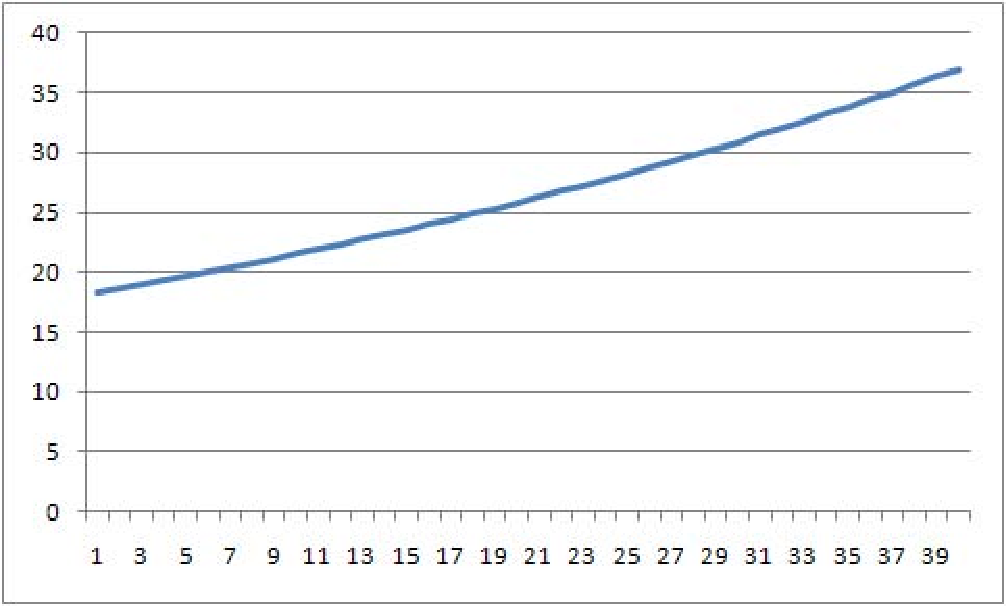
\includegraphics{improve2.pdf}}
% GNUPLOT: LaTeX picture
\setlength{\unitlength}{0.240900pt}
\ifx\plotpoint\undefined\newsavebox{\plotpoint}\fi
\begin{picture}(1500,900)(0,0)
\sbox{\plotpoint}{\rule[-0.200pt]{0.400pt}{0.400pt}}%
\put(131.0,131.0){\rule[-0.200pt]{4.818pt}{0.400pt}}
\put(111,131){\makebox(0,0)[r]{10}}
\put(1419.0,131.0){\rule[-0.200pt]{4.818pt}{0.400pt}}
\put(131.0,252.0){\rule[-0.200pt]{4.818pt}{0.400pt}}
\put(111,252){\makebox(0,0)[r]{15}}
\put(1419.0,252.0){\rule[-0.200pt]{4.818pt}{0.400pt}}
\put(131.0,374.0){\rule[-0.200pt]{4.818pt}{0.400pt}}
\put(111,374){\makebox(0,0)[r]{20}}
\put(1419.0,374.0){\rule[-0.200pt]{4.818pt}{0.400pt}}
\put(131.0,495.0){\rule[-0.200pt]{4.818pt}{0.400pt}}
\put(111,495){\makebox(0,0)[r]{25}}
\put(1419.0,495.0){\rule[-0.200pt]{4.818pt}{0.400pt}}
\put(131.0,616.0){\rule[-0.200pt]{4.818pt}{0.400pt}}
\put(111,616){\makebox(0,0)[r]{30}}
\put(1419.0,616.0){\rule[-0.200pt]{4.818pt}{0.400pt}}
\put(131.0,738.0){\rule[-0.200pt]{4.818pt}{0.400pt}}
\put(111,738){\makebox(0,0)[r]{35}}
\put(1419.0,738.0){\rule[-0.200pt]{4.818pt}{0.400pt}}
\put(131.0,859.0){\rule[-0.200pt]{4.818pt}{0.400pt}}
\put(111,859){\makebox(0,0)[r]{40}}
\put(1419.0,859.0){\rule[-0.200pt]{4.818pt}{0.400pt}}
\put(131.0,131.0){\rule[-0.200pt]{0.400pt}{4.818pt}}
\put(131,90){\makebox(0,0){ 1}}
\put(131.0,839.0){\rule[-0.200pt]{0.400pt}{4.818pt}}
\put(198.0,131.0){\rule[-0.200pt]{0.400pt}{4.818pt}}
\put(198,90){\makebox(0,0){ 3}}
\put(198.0,839.0){\rule[-0.200pt]{0.400pt}{4.818pt}}
\put(265.0,131.0){\rule[-0.200pt]{0.400pt}{4.818pt}}
\put(265,90){\makebox(0,0){ 5}}
\put(265.0,839.0){\rule[-0.200pt]{0.400pt}{4.818pt}}
\put(332.0,131.0){\rule[-0.200pt]{0.400pt}{4.818pt}}
\put(332,90){\makebox(0,0){ 7}}
\put(332.0,839.0){\rule[-0.200pt]{0.400pt}{4.818pt}}
\put(399.0,131.0){\rule[-0.200pt]{0.400pt}{4.818pt}}
\put(399,90){\makebox(0,0){ 9}}
\put(399.0,839.0){\rule[-0.200pt]{0.400pt}{4.818pt}}
\put(466.0,131.0){\rule[-0.200pt]{0.400pt}{4.818pt}}
\put(466,90){\makebox(0,0){ 11}}
\put(466.0,839.0){\rule[-0.200pt]{0.400pt}{4.818pt}}
\put(533.0,131.0){\rule[-0.200pt]{0.400pt}{4.818pt}}
\put(533,90){\makebox(0,0){ 13}}
\put(533.0,839.0){\rule[-0.200pt]{0.400pt}{4.818pt}}
\put(601.0,131.0){\rule[-0.200pt]{0.400pt}{4.818pt}}
\put(601,90){\makebox(0,0){ 15}}
\put(601.0,839.0){\rule[-0.200pt]{0.400pt}{4.818pt}}
\put(668.0,131.0){\rule[-0.200pt]{0.400pt}{4.818pt}}
\put(668,90){\makebox(0,0){ 17}}
\put(668.0,839.0){\rule[-0.200pt]{0.400pt}{4.818pt}}
\put(735.0,131.0){\rule[-0.200pt]{0.400pt}{4.818pt}}
\put(735,90){\makebox(0,0){ 19}}
\put(735.0,839.0){\rule[-0.200pt]{0.400pt}{4.818pt}}
\put(802.0,131.0){\rule[-0.200pt]{0.400pt}{4.818pt}}
\put(802,90){\makebox(0,0){ 21}}
\put(802.0,839.0){\rule[-0.200pt]{0.400pt}{4.818pt}}
\put(869.0,131.0){\rule[-0.200pt]{0.400pt}{4.818pt}}
\put(869,90){\makebox(0,0){ 23}}
\put(869.0,839.0){\rule[-0.200pt]{0.400pt}{4.818pt}}
\put(936.0,131.0){\rule[-0.200pt]{0.400pt}{4.818pt}}
\put(936,90){\makebox(0,0){ 25}}
\put(936.0,839.0){\rule[-0.200pt]{0.400pt}{4.818pt}}
\put(1003.0,131.0){\rule[-0.200pt]{0.400pt}{4.818pt}}
\put(1003,90){\makebox(0,0){ 27}}
\put(1003.0,839.0){\rule[-0.200pt]{0.400pt}{4.818pt}}
\put(1070.0,131.0){\rule[-0.200pt]{0.400pt}{4.818pt}}
\put(1070,90){\makebox(0,0){ 29}}
\put(1070.0,839.0){\rule[-0.200pt]{0.400pt}{4.818pt}}
\put(1137.0,131.0){\rule[-0.200pt]{0.400pt}{4.818pt}}
\put(1137,90){\makebox(0,0){ 31}}
\put(1137.0,839.0){\rule[-0.200pt]{0.400pt}{4.818pt}}
\put(1204.0,131.0){\rule[-0.200pt]{0.400pt}{4.818pt}}
\put(1204,90){\makebox(0,0){ 33}}
\put(1204.0,839.0){\rule[-0.200pt]{0.400pt}{4.818pt}}
\put(1271.0,131.0){\rule[-0.200pt]{0.400pt}{4.818pt}}
\put(1271,90){\makebox(0,0){ 35}}
\put(1271.0,839.0){\rule[-0.200pt]{0.400pt}{4.818pt}}
\put(1338.0,131.0){\rule[-0.200pt]{0.400pt}{4.818pt}}
\put(1338,90){\makebox(0,0){ 37}}
\put(1338.0,839.0){\rule[-0.200pt]{0.400pt}{4.818pt}}
\put(1405.0,131.0){\rule[-0.200pt]{0.400pt}{4.818pt}}
\put(1405,90){\makebox(0,0){ 39}}
\put(1405.0,839.0){\rule[-0.200pt]{0.400pt}{4.818pt}}
\put(131.0,131.0){\rule[-0.200pt]{0.400pt}{175.375pt}}
\put(131.0,131.0){\rule[-0.200pt]{315.097pt}{0.400pt}}
\put(1439.0,131.0){\rule[-0.200pt]{0.400pt}{175.375pt}}
\put(131.0,859.0){\rule[-0.200pt]{315.097pt}{0.400pt}}
\put(30,495){\makebox(0,0){\rotatebox{90}{用户贡献}}}
\put(785,-10){\makebox(0,0){月度}}
\put(1279,819){\makebox(0,0)[r]{仿真数据}}
\put(1299.0,819.0){\rule[-0.200pt]{24.090pt}{0.400pt}}
\put(131,184){\usebox{\plotpoint}}
\multiput(131.58,184.00)(0.498,1.242){65}{\rule{0.120pt}{1.088pt}}
\multiput(130.17,184.00)(34.000,81.741){2}{\rule{0.400pt}{0.544pt}}
\multiput(165.58,268.00)(0.497,0.744){63}{\rule{0.120pt}{0.694pt}}
\multiput(164.17,268.00)(33.000,47.560){2}{\rule{0.400pt}{0.347pt}}
\multiput(198.58,317.00)(0.498,0.514){65}{\rule{0.120pt}{0.512pt}}
\multiput(197.17,317.00)(34.000,33.938){2}{\rule{0.400pt}{0.256pt}}
\multiput(232.00,352.58)(0.635,0.497){49}{\rule{0.608pt}{0.120pt}}
\multiput(232.00,351.17)(31.739,26.000){2}{\rule{0.304pt}{0.400pt}}
\multiput(265.00,378.58)(0.775,0.496){41}{\rule{0.718pt}{0.120pt}}
\multiput(265.00,377.17)(32.509,22.000){2}{\rule{0.359pt}{0.400pt}}
\multiput(299.00,400.58)(0.874,0.495){35}{\rule{0.795pt}{0.119pt}}
\multiput(299.00,399.17)(31.350,19.000){2}{\rule{0.397pt}{0.400pt}}
\multiput(332.00,419.58)(1.073,0.494){29}{\rule{0.950pt}{0.119pt}}
\multiput(332.00,418.17)(32.028,16.000){2}{\rule{0.475pt}{0.400pt}}
\multiput(366.00,435.58)(1.195,0.494){25}{\rule{1.043pt}{0.119pt}}
\multiput(366.00,434.17)(30.835,14.000){2}{\rule{0.521pt}{0.400pt}}
\multiput(399.00,449.58)(1.329,0.493){23}{\rule{1.146pt}{0.119pt}}
\multiput(399.00,448.17)(31.621,13.000){2}{\rule{0.573pt}{0.400pt}}
\multiput(433.00,462.58)(1.401,0.492){21}{\rule{1.200pt}{0.119pt}}
\multiput(433.00,461.17)(30.509,12.000){2}{\rule{0.600pt}{0.400pt}}
\multiput(466.00,474.58)(1.746,0.491){17}{\rule{1.460pt}{0.118pt}}
\multiput(466.00,473.17)(30.970,10.000){2}{\rule{0.730pt}{0.400pt}}
\multiput(500.00,484.58)(1.694,0.491){17}{\rule{1.420pt}{0.118pt}}
\multiput(500.00,483.17)(30.053,10.000){2}{\rule{0.710pt}{0.400pt}}
\multiput(533.00,494.59)(1.951,0.489){15}{\rule{1.611pt}{0.118pt}}
\multiput(533.00,493.17)(30.656,9.000){2}{\rule{0.806pt}{0.400pt}}
\multiput(567.00,503.59)(2.211,0.488){13}{\rule{1.800pt}{0.117pt}}
\multiput(567.00,502.17)(30.264,8.000){2}{\rule{0.900pt}{0.400pt}}
\multiput(601.00,511.59)(2.145,0.488){13}{\rule{1.750pt}{0.117pt}}
\multiput(601.00,510.17)(29.368,8.000){2}{\rule{0.875pt}{0.400pt}}
\multiput(634.00,519.59)(2.552,0.485){11}{\rule{2.043pt}{0.117pt}}
\multiput(634.00,518.17)(29.760,7.000){2}{\rule{1.021pt}{0.400pt}}
\multiput(668.00,526.59)(2.476,0.485){11}{\rule{1.986pt}{0.117pt}}
\multiput(668.00,525.17)(28.879,7.000){2}{\rule{0.993pt}{0.400pt}}
\multiput(701.00,533.59)(2.552,0.485){11}{\rule{2.043pt}{0.117pt}}
\multiput(701.00,532.17)(29.760,7.000){2}{\rule{1.021pt}{0.400pt}}
\multiput(735.00,540.59)(2.932,0.482){9}{\rule{2.300pt}{0.116pt}}
\multiput(735.00,539.17)(28.226,6.000){2}{\rule{1.150pt}{0.400pt}}
\multiput(768.00,546.59)(3.022,0.482){9}{\rule{2.367pt}{0.116pt}}
\multiput(768.00,545.17)(29.088,6.000){2}{\rule{1.183pt}{0.400pt}}
\multiput(802.00,552.59)(3.604,0.477){7}{\rule{2.740pt}{0.115pt}}
\multiput(802.00,551.17)(27.313,5.000){2}{\rule{1.370pt}{0.400pt}}
\multiput(835.00,557.59)(3.022,0.482){9}{\rule{2.367pt}{0.116pt}}
\multiput(835.00,556.17)(29.088,6.000){2}{\rule{1.183pt}{0.400pt}}
\multiput(869.00,563.59)(3.604,0.477){7}{\rule{2.740pt}{0.115pt}}
\multiput(869.00,562.17)(27.313,5.000){2}{\rule{1.370pt}{0.400pt}}
\multiput(902.00,568.59)(3.716,0.477){7}{\rule{2.820pt}{0.115pt}}
\multiput(902.00,567.17)(28.147,5.000){2}{\rule{1.410pt}{0.400pt}}
\multiput(936.00,573.60)(4.722,0.468){5}{\rule{3.400pt}{0.113pt}}
\multiput(936.00,572.17)(25.943,4.000){2}{\rule{1.700pt}{0.400pt}}
\multiput(969.00,577.59)(3.716,0.477){7}{\rule{2.820pt}{0.115pt}}
\multiput(969.00,576.17)(28.147,5.000){2}{\rule{1.410pt}{0.400pt}}
\multiput(1003.00,582.60)(4.868,0.468){5}{\rule{3.500pt}{0.113pt}}
\multiput(1003.00,581.17)(26.736,4.000){2}{\rule{1.750pt}{0.400pt}}
\multiput(1037.00,586.59)(3.604,0.477){7}{\rule{2.740pt}{0.115pt}}
\multiput(1037.00,585.17)(27.313,5.000){2}{\rule{1.370pt}{0.400pt}}
\multiput(1070.00,591.60)(4.868,0.468){5}{\rule{3.500pt}{0.113pt}}
\multiput(1070.00,590.17)(26.736,4.000){2}{\rule{1.750pt}{0.400pt}}
\multiput(1104.00,595.60)(4.722,0.468){5}{\rule{3.400pt}{0.113pt}}
\multiput(1104.00,594.17)(25.943,4.000){2}{\rule{1.700pt}{0.400pt}}
\multiput(1137.00,599.60)(4.868,0.468){5}{\rule{3.500pt}{0.113pt}}
\multiput(1137.00,598.17)(26.736,4.000){2}{\rule{1.750pt}{0.400pt}}
\multiput(1171.00,603.61)(7.160,0.447){3}{\rule{4.500pt}{0.108pt}}
\multiput(1171.00,602.17)(23.660,3.000){2}{\rule{2.250pt}{0.400pt}}
\multiput(1204.00,606.60)(4.868,0.468){5}{\rule{3.500pt}{0.113pt}}
\multiput(1204.00,605.17)(26.736,4.000){2}{\rule{1.750pt}{0.400pt}}
\multiput(1238.00,610.61)(7.160,0.447){3}{\rule{4.500pt}{0.108pt}}
\multiput(1238.00,609.17)(23.660,3.000){2}{\rule{2.250pt}{0.400pt}}
\multiput(1271.00,613.60)(4.868,0.468){5}{\rule{3.500pt}{0.113pt}}
\multiput(1271.00,612.17)(26.736,4.000){2}{\rule{1.750pt}{0.400pt}}
\multiput(1305.00,617.61)(7.160,0.447){3}{\rule{4.500pt}{0.108pt}}
\multiput(1305.00,616.17)(23.660,3.000){2}{\rule{2.250pt}{0.400pt}}
\multiput(1338.00,620.61)(7.383,0.447){3}{\rule{4.633pt}{0.108pt}}
\multiput(1338.00,619.17)(24.383,3.000){2}{\rule{2.317pt}{0.400pt}}
\multiput(1372.00,623.61)(7.160,0.447){3}{\rule{4.500pt}{0.108pt}}
\multiput(1372.00,622.17)(23.660,3.000){2}{\rule{2.250pt}{0.400pt}}
\multiput(1405.00,626.61)(7.383,0.447){3}{\rule{4.633pt}{0.108pt}}
\multiput(1405.00,625.17)(24.383,3.000){2}{\rule{2.317pt}{0.400pt}}
\put(131,184){\makebox(0,0){$+$}}
\put(165,268){\makebox(0,0){$+$}}
\put(198,317){\makebox(0,0){$+$}}
\put(232,352){\makebox(0,0){$+$}}
\put(265,378){\makebox(0,0){$+$}}
\put(299,400){\makebox(0,0){$+$}}
\put(332,419){\makebox(0,0){$+$}}
\put(366,435){\makebox(0,0){$+$}}
\put(399,449){\makebox(0,0){$+$}}
\put(433,462){\makebox(0,0){$+$}}
\put(466,474){\makebox(0,0){$+$}}
\put(500,484){\makebox(0,0){$+$}}
\put(533,494){\makebox(0,0){$+$}}
\put(567,503){\makebox(0,0){$+$}}
\put(601,511){\makebox(0,0){$+$}}
\put(634,519){\makebox(0,0){$+$}}
\put(668,526){\makebox(0,0){$+$}}
\put(701,533){\makebox(0,0){$+$}}
\put(735,540){\makebox(0,0){$+$}}
\put(768,546){\makebox(0,0){$+$}}
\put(802,552){\makebox(0,0){$+$}}
\put(835,557){\makebox(0,0){$+$}}
\put(869,563){\makebox(0,0){$+$}}
\put(902,568){\makebox(0,0){$+$}}
\put(936,573){\makebox(0,0){$+$}}
\put(969,577){\makebox(0,0){$+$}}
\put(1003,582){\makebox(0,0){$+$}}
\put(1037,586){\makebox(0,0){$+$}}
\put(1070,591){\makebox(0,0){$+$}}
\put(1104,595){\makebox(0,0){$+$}}
\put(1137,599){\makebox(0,0){$+$}}
\put(1171,603){\makebox(0,0){$+$}}
\put(1204,606){\makebox(0,0){$+$}}
\put(1238,610){\makebox(0,0){$+$}}
\put(1271,613){\makebox(0,0){$+$}}
\put(1305,617){\makebox(0,0){$+$}}
\put(1338,620){\makebox(0,0){$+$}}
\put(1372,623){\makebox(0,0){$+$}}
\put(1405,626){\makebox(0,0){$+$}}
\put(1439,629){\makebox(0,0){$+$}}
\put(1349,819){\makebox(0,0){$+$}}
\put(1279,768){\makebox(0,0)[r]{改进数据}}
\put(1299.0,768.0){\rule[-0.200pt]{24.090pt}{0.400pt}}
\put(131,333){\usebox{\plotpoint}}
\multiput(131.00,333.59)(2.211,0.488){13}{\rule{1.800pt}{0.117pt}}
\multiput(131.00,332.17)(30.264,8.000){2}{\rule{0.900pt}{0.400pt}}
\multiput(165.00,341.59)(2.145,0.488){13}{\rule{1.750pt}{0.117pt}}
\multiput(165.00,340.17)(29.368,8.000){2}{\rule{0.875pt}{0.400pt}}
\multiput(198.00,349.59)(1.951,0.489){15}{\rule{1.611pt}{0.118pt}}
\multiput(198.00,348.17)(30.656,9.000){2}{\rule{0.806pt}{0.400pt}}
\multiput(232.00,358.59)(2.145,0.488){13}{\rule{1.750pt}{0.117pt}}
\multiput(232.00,357.17)(29.368,8.000){2}{\rule{0.875pt}{0.400pt}}
\multiput(265.00,366.59)(1.951,0.489){15}{\rule{1.611pt}{0.118pt}}
\multiput(265.00,365.17)(30.656,9.000){2}{\rule{0.806pt}{0.400pt}}
\multiput(299.00,375.59)(1.893,0.489){15}{\rule{1.567pt}{0.118pt}}
\multiput(299.00,374.17)(29.748,9.000){2}{\rule{0.783pt}{0.400pt}}
\multiput(332.00,384.59)(1.951,0.489){15}{\rule{1.611pt}{0.118pt}}
\multiput(332.00,383.17)(30.656,9.000){2}{\rule{0.806pt}{0.400pt}}
\multiput(366.00,393.59)(1.893,0.489){15}{\rule{1.567pt}{0.118pt}}
\multiput(366.00,392.17)(29.748,9.000){2}{\rule{0.783pt}{0.400pt}}
\multiput(399.00,402.59)(1.951,0.489){15}{\rule{1.611pt}{0.118pt}}
\multiput(399.00,401.17)(30.656,9.000){2}{\rule{0.806pt}{0.400pt}}
\multiput(433.00,411.58)(1.694,0.491){17}{\rule{1.420pt}{0.118pt}}
\multiput(433.00,410.17)(30.053,10.000){2}{\rule{0.710pt}{0.400pt}}
\multiput(466.00,421.59)(1.951,0.489){15}{\rule{1.611pt}{0.118pt}}
\multiput(466.00,420.17)(30.656,9.000){2}{\rule{0.806pt}{0.400pt}}
\multiput(500.00,430.58)(1.694,0.491){17}{\rule{1.420pt}{0.118pt}}
\multiput(500.00,429.17)(30.053,10.000){2}{\rule{0.710pt}{0.400pt}}
\multiput(533.00,440.58)(1.746,0.491){17}{\rule{1.460pt}{0.118pt}}
\multiput(533.00,439.17)(30.970,10.000){2}{\rule{0.730pt}{0.400pt}}
\multiput(567.00,450.58)(1.581,0.492){19}{\rule{1.336pt}{0.118pt}}
\multiput(567.00,449.17)(31.226,11.000){2}{\rule{0.668pt}{0.400pt}}
\multiput(601.00,461.58)(1.694,0.491){17}{\rule{1.420pt}{0.118pt}}
\multiput(601.00,460.17)(30.053,10.000){2}{\rule{0.710pt}{0.400pt}}
\multiput(634.00,471.58)(1.746,0.491){17}{\rule{1.460pt}{0.118pt}}
\multiput(634.00,470.17)(30.970,10.000){2}{\rule{0.730pt}{0.400pt}}
\multiput(668.00,481.58)(1.534,0.492){19}{\rule{1.300pt}{0.118pt}}
\multiput(668.00,480.17)(30.302,11.000){2}{\rule{0.650pt}{0.400pt}}
\multiput(701.00,492.58)(1.581,0.492){19}{\rule{1.336pt}{0.118pt}}
\multiput(701.00,491.17)(31.226,11.000){2}{\rule{0.668pt}{0.400pt}}
\multiput(735.00,503.58)(1.534,0.492){19}{\rule{1.300pt}{0.118pt}}
\multiput(735.00,502.17)(30.302,11.000){2}{\rule{0.650pt}{0.400pt}}
\multiput(768.00,514.58)(1.444,0.492){21}{\rule{1.233pt}{0.119pt}}
\multiput(768.00,513.17)(31.440,12.000){2}{\rule{0.617pt}{0.400pt}}
\multiput(802.00,526.58)(1.534,0.492){19}{\rule{1.300pt}{0.118pt}}
\multiput(802.00,525.17)(30.302,11.000){2}{\rule{0.650pt}{0.400pt}}
\multiput(835.00,537.58)(1.444,0.492){21}{\rule{1.233pt}{0.119pt}}
\multiput(835.00,536.17)(31.440,12.000){2}{\rule{0.617pt}{0.400pt}}
\multiput(869.00,549.58)(1.401,0.492){21}{\rule{1.200pt}{0.119pt}}
\multiput(869.00,548.17)(30.509,12.000){2}{\rule{0.600pt}{0.400pt}}
\multiput(902.00,561.58)(1.444,0.492){21}{\rule{1.233pt}{0.119pt}}
\multiput(902.00,560.17)(31.440,12.000){2}{\rule{0.617pt}{0.400pt}}
\multiput(936.00,573.58)(1.290,0.493){23}{\rule{1.115pt}{0.119pt}}
\multiput(936.00,572.17)(30.685,13.000){2}{\rule{0.558pt}{0.400pt}}
\multiput(969.00,586.58)(1.444,0.492){21}{\rule{1.233pt}{0.119pt}}
\multiput(969.00,585.17)(31.440,12.000){2}{\rule{0.617pt}{0.400pt}}
\multiput(1003.00,598.58)(1.329,0.493){23}{\rule{1.146pt}{0.119pt}}
\multiput(1003.00,597.17)(31.621,13.000){2}{\rule{0.573pt}{0.400pt}}
\multiput(1037.00,611.58)(1.195,0.494){25}{\rule{1.043pt}{0.119pt}}
\multiput(1037.00,610.17)(30.835,14.000){2}{\rule{0.521pt}{0.400pt}}
\multiput(1070.00,625.58)(1.329,0.493){23}{\rule{1.146pt}{0.119pt}}
\multiput(1070.00,624.17)(31.621,13.000){2}{\rule{0.573pt}{0.400pt}}
\multiput(1104.00,638.58)(1.195,0.494){25}{\rule{1.043pt}{0.119pt}}
\multiput(1104.00,637.17)(30.835,14.000){2}{\rule{0.521pt}{0.400pt}}
\multiput(1137.00,652.58)(1.329,0.493){23}{\rule{1.146pt}{0.119pt}}
\multiput(1137.00,651.17)(31.621,13.000){2}{\rule{0.573pt}{0.400pt}}
\multiput(1171.00,665.58)(1.195,0.494){25}{\rule{1.043pt}{0.119pt}}
\multiput(1171.00,664.17)(30.835,14.000){2}{\rule{0.521pt}{0.400pt}}
\multiput(1204.00,679.58)(1.147,0.494){27}{\rule{1.007pt}{0.119pt}}
\multiput(1204.00,678.17)(31.911,15.000){2}{\rule{0.503pt}{0.400pt}}
\multiput(1238.00,694.58)(1.113,0.494){27}{\rule{0.980pt}{0.119pt}}
\multiput(1238.00,693.17)(30.966,15.000){2}{\rule{0.490pt}{0.400pt}}
\multiput(1271.00,709.58)(1.231,0.494){25}{\rule{1.071pt}{0.119pt}}
\multiput(1271.00,708.17)(31.776,14.000){2}{\rule{0.536pt}{0.400pt}}
\multiput(1305.00,723.58)(1.041,0.494){29}{\rule{0.925pt}{0.119pt}}
\multiput(1305.00,722.17)(31.080,16.000){2}{\rule{0.463pt}{0.400pt}}
\multiput(1338.00,739.58)(1.147,0.494){27}{\rule{1.007pt}{0.119pt}}
\multiput(1338.00,738.17)(31.911,15.000){2}{\rule{0.503pt}{0.400pt}}
\multiput(1372.00,754.58)(1.041,0.494){29}{\rule{0.925pt}{0.119pt}}
\multiput(1372.00,753.17)(31.080,16.000){2}{\rule{0.463pt}{0.400pt}}
\multiput(1405.00,770.58)(1.073,0.494){29}{\rule{0.950pt}{0.119pt}}
\multiput(1405.00,769.17)(32.028,16.000){2}{\rule{0.475pt}{0.400pt}}
\put(131,333){\makebox(0,0){$\times$}}
\put(165,341){\makebox(0,0){$\times$}}
\put(198,349){\makebox(0,0){$\times$}}
\put(232,358){\makebox(0,0){$\times$}}
\put(265,366){\makebox(0,0){$\times$}}
\put(299,375){\makebox(0,0){$\times$}}
\put(332,384){\makebox(0,0){$\times$}}
\put(366,393){\makebox(0,0){$\times$}}
\put(399,402){\makebox(0,0){$\times$}}
\put(433,411){\makebox(0,0){$\times$}}
\put(466,421){\makebox(0,0){$\times$}}
\put(500,430){\makebox(0,0){$\times$}}
\put(533,440){\makebox(0,0){$\times$}}
\put(567,450){\makebox(0,0){$\times$}}
\put(601,461){\makebox(0,0){$\times$}}
\put(634,471){\makebox(0,0){$\times$}}
\put(668,481){\makebox(0,0){$\times$}}
\put(701,492){\makebox(0,0){$\times$}}
\put(735,503){\makebox(0,0){$\times$}}
\put(768,514){\makebox(0,0){$\times$}}
\put(802,526){\makebox(0,0){$\times$}}
\put(835,537){\makebox(0,0){$\times$}}
\put(869,549){\makebox(0,0){$\times$}}
\put(902,561){\makebox(0,0){$\times$}}
\put(936,573){\makebox(0,0){$\times$}}
\put(969,586){\makebox(0,0){$\times$}}
\put(1003,598){\makebox(0,0){$\times$}}
\put(1037,611){\makebox(0,0){$\times$}}
\put(1070,625){\makebox(0,0){$\times$}}
\put(1104,638){\makebox(0,0){$\times$}}
\put(1137,652){\makebox(0,0){$\times$}}
\put(1171,665){\makebox(0,0){$\times$}}
\put(1204,679){\makebox(0,0){$\times$}}
\put(1238,694){\makebox(0,0){$\times$}}
\put(1271,709){\makebox(0,0){$\times$}}
\put(1305,723){\makebox(0,0){$\times$}}
\put(1338,739){\makebox(0,0){$\times$}}
\put(1372,754){\makebox(0,0){$\times$}}
\put(1405,770){\makebox(0,0){$\times$}}
\put(1439,786){\makebox(0,0){$\times$}}
\put(1349,778){\makebox(0,0){$\times$}}
\put(131.0,131.0){\rule[-0.200pt]{0.400pt}{175.375pt}}
\put(131.0,131.0){\rule[-0.200pt]{315.097pt}{0.400pt}}
\put(1439.0,131.0){\rule[-0.200pt]{0.400pt}{175.375pt}}
\put(131.0,859.0){\rule[-0.200pt]{315.097pt}{0.400pt}}
\end{picture}
  
\caption{\small{\textbf{提升领导者用户最大工作时间的仿真结果}}}
  \label{fig:improve2}
\end{figure}

在提升了个体的最大工作时间后,个体的贡献显著增长,同时增长的速度呈增加
的趋势。这证明了个体的协同行为确实受到了该因素的制约,使得贡献形成了S
型增长。随着时间推移,个体的贡献将稳定维持在一个较高的水平,除非外界因
素发
生明显的变化,否则不会发生太大的波动。

领导者用户主要受到个体层次的动机驱动参与知识协同,他们在很短的时间内就
达到了个人能力的最大值。为了维持领导者用户的参与水平,社区所能采取的措施和其他群体
有显著的不同。激励措施对于领导者用户并不重要,即使动机水平再高也不能提
升其参与程度。社区所要做的应该是保护用户的热情,不要使社区中的一些负面
因素降低参与者的动机。领导者用户是真正希望从工作中获得快乐的一类用户,
如果他们不能从中获得满足感,则参与动机会很快消失。为此,社区应该多听取
用户意见,把握好社区发展的方向,尽力满足用户需求,努力维护用户的动机不
受到伤害。同时社区应该注意到,尽管领导者用户是社区的核心力量,但是其他
类型用户的作用也不应该被忽视。如果社区不能平衡核心用户的需求和其他成员
的利益,那么社区的发展会受到很大的制约。

\subsection{领域专家用户}
领域专家用户同领导者用户有着相似的协同模式,同时他们对于所参与的条目也
有极高的贡献度。但是,领域专家用户的月人均贡献却和领导者用户大相径庭,
不但数值很低,而且呈递减趋势,最后到1左右稳定下来。贡献度的下降趋势显
示了对数函数的特征,模型仿真的结果说明用户协同贡献的变化符合寻的模式,即负反馈成
为了领域专家动机和行为间关系的主导关系。

在因果模型中存在两个负反馈环:一个是个体最大工作时间的负反馈环,另一个
是成就动机的负反馈环。前者限制了协同行为的最大水平,后者则有可能改变整
个因果链的主导关系。考虑到领域专家用户的月人均贡献非常低,因此决定行为
模式的负反馈环是最大工作时间的可能性不大,也就是说用户的实际能力还远远
没有发挥出来。真正影响用户协同水平的是成就动机。成就需求在个体完成任务
的过程中得到满足,这种满足感会削弱成就动机,从而降低个体的协同参与水平。
成就动机成为主导的负反馈环有两个必要条件:首先成就动机的初始值必须很
高,这样成就动机的重要性才能超过其他动机;其次满足感必须持续处于较高水
平,也就是成就感的流失非常慢。只有这样,个体的动机才会以成就动机为主,
同时成就需求可以在较长时间段内得到满足,降低了个体的协同行为水平。 

以上推断可以利用仿真来验证。图\ref{fig:improve4}是将领域专家用户所有的
动机因素水平提升$20\%$后得到的结果。结果显示用户的协同水平有所提高,说
明提升动机因素水平是有作用的。但是,协同水平的变化趋势仍然没有改变,还
是呈现缓慢下降的趋势。这意味着负反馈的力量依然强大。消除负反馈的影响而
不是激励用户提升其动机水平是改进领域专家用户绩效行之有效的方法。
\begin{figure}[!htb]
  \centering
%  \scalebox{0.65}{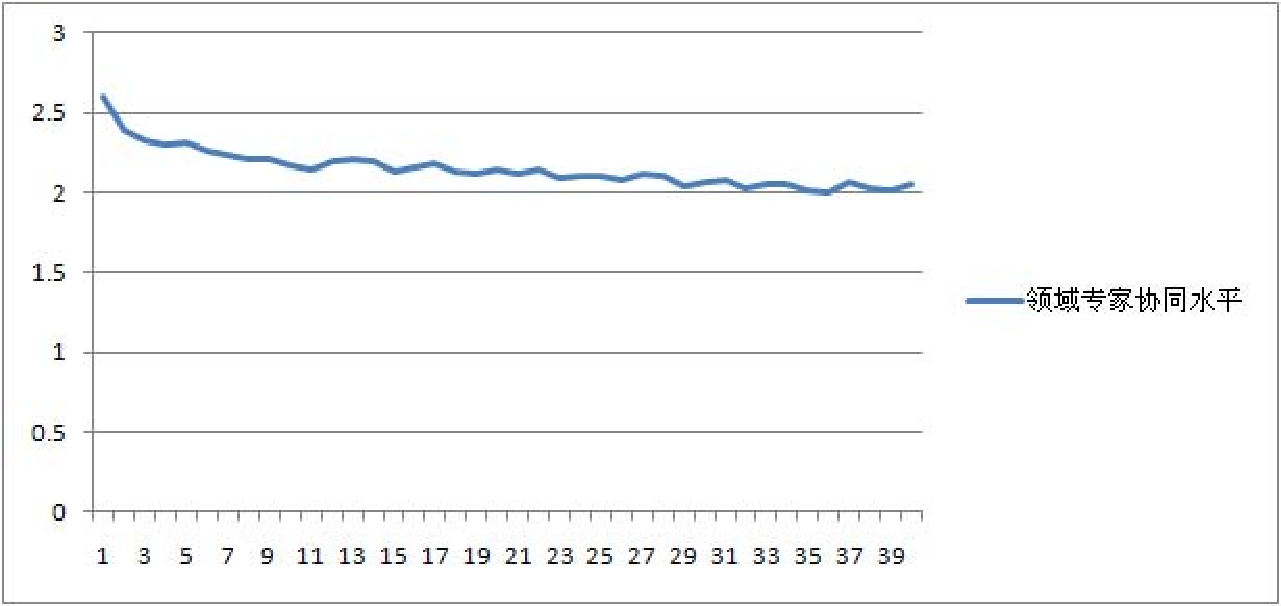
\includegraphics{improve4.pdf}}
  % GNUPLOT: LaTeX picture
\setlength{\unitlength}{0.240900pt}
\ifx\plotpoint\undefined\newsavebox{\plotpoint}\fi
\begin{picture}(1500,900)(0,0)
\sbox{\plotpoint}{\rule[-0.200pt]{0.400pt}{0.400pt}}%
\put(131.0,82.0){\rule[-0.200pt]{4.818pt}{0.400pt}}
\put(111,82){\makebox(0,0)[r]{ 0}}
\put(1419.0,82.0){\rule[-0.200pt]{4.818pt}{0.400pt}}
\put(131.0,276.0){\rule[-0.200pt]{4.818pt}{0.400pt}}
\put(111,276){\makebox(0,0)[r]{ 1}}
\put(1419.0,276.0){\rule[-0.200pt]{4.818pt}{0.400pt}}
\put(131.0,471.0){\rule[-0.200pt]{4.818pt}{0.400pt}}
\put(111,471){\makebox(0,0)[r]{ 2}}
\put(1419.0,471.0){\rule[-0.200pt]{4.818pt}{0.400pt}}
\put(131.0,665.0){\rule[-0.200pt]{4.818pt}{0.400pt}}
\put(111,665){\makebox(0,0)[r]{ 3}}
\put(1419.0,665.0){\rule[-0.200pt]{4.818pt}{0.400pt}}
\put(131.0,82.0){\rule[-0.200pt]{0.400pt}{4.818pt}}
\put(131,41){\makebox(0,0){ 1}}
\put(131.0,839.0){\rule[-0.200pt]{0.400pt}{4.818pt}}
\put(198.0,82.0){\rule[-0.200pt]{0.400pt}{4.818pt}}
\put(198,41){\makebox(0,0){ 3}}
\put(198.0,839.0){\rule[-0.200pt]{0.400pt}{4.818pt}}
\put(265.0,82.0){\rule[-0.200pt]{0.400pt}{4.818pt}}
\put(265,41){\makebox(0,0){ 5}}
\put(265.0,839.0){\rule[-0.200pt]{0.400pt}{4.818pt}}
\put(332.0,82.0){\rule[-0.200pt]{0.400pt}{4.818pt}}
\put(332,41){\makebox(0,0){ 7}}
\put(332.0,839.0){\rule[-0.200pt]{0.400pt}{4.818pt}}
\put(399.0,82.0){\rule[-0.200pt]{0.400pt}{4.818pt}}
\put(399,41){\makebox(0,0){ 9}}
\put(399.0,839.0){\rule[-0.200pt]{0.400pt}{4.818pt}}
\put(466.0,82.0){\rule[-0.200pt]{0.400pt}{4.818pt}}
\put(466,41){\makebox(0,0){ 11}}
\put(466.0,839.0){\rule[-0.200pt]{0.400pt}{4.818pt}}
\put(533.0,82.0){\rule[-0.200pt]{0.400pt}{4.818pt}}
\put(533,41){\makebox(0,0){ 13}}
\put(533.0,839.0){\rule[-0.200pt]{0.400pt}{4.818pt}}
\put(601.0,82.0){\rule[-0.200pt]{0.400pt}{4.818pt}}
\put(601,41){\makebox(0,0){ 15}}
\put(601.0,839.0){\rule[-0.200pt]{0.400pt}{4.818pt}}
\put(668.0,82.0){\rule[-0.200pt]{0.400pt}{4.818pt}}
\put(668,41){\makebox(0,0){ 17}}
\put(668.0,839.0){\rule[-0.200pt]{0.400pt}{4.818pt}}
\put(735.0,82.0){\rule[-0.200pt]{0.400pt}{4.818pt}}
\put(735,41){\makebox(0,0){ 19}}
\put(735.0,839.0){\rule[-0.200pt]{0.400pt}{4.818pt}}
\put(802.0,82.0){\rule[-0.200pt]{0.400pt}{4.818pt}}
\put(802,41){\makebox(0,0){ 21}}
\put(802.0,839.0){\rule[-0.200pt]{0.400pt}{4.818pt}}
\put(869.0,82.0){\rule[-0.200pt]{0.400pt}{4.818pt}}
\put(869,41){\makebox(0,0){ 23}}
\put(869.0,839.0){\rule[-0.200pt]{0.400pt}{4.818pt}}
\put(936.0,82.0){\rule[-0.200pt]{0.400pt}{4.818pt}}
\put(936,41){\makebox(0,0){ 25}}
\put(936.0,839.0){\rule[-0.200pt]{0.400pt}{4.818pt}}
\put(1003.0,82.0){\rule[-0.200pt]{0.400pt}{4.818pt}}
\put(1003,41){\makebox(0,0){ 27}}
\put(1003.0,839.0){\rule[-0.200pt]{0.400pt}{4.818pt}}
\put(1070.0,82.0){\rule[-0.200pt]{0.400pt}{4.818pt}}
\put(1070,41){\makebox(0,0){ 29}}
\put(1070.0,839.0){\rule[-0.200pt]{0.400pt}{4.818pt}}
\put(1137.0,82.0){\rule[-0.200pt]{0.400pt}{4.818pt}}
\put(1137,41){\makebox(0,0){ 31}}
\put(1137.0,839.0){\rule[-0.200pt]{0.400pt}{4.818pt}}
\put(1204.0,82.0){\rule[-0.200pt]{0.400pt}{4.818pt}}
\put(1204,41){\makebox(0,0){ 33}}
\put(1204.0,839.0){\rule[-0.200pt]{0.400pt}{4.818pt}}
\put(1271.0,82.0){\rule[-0.200pt]{0.400pt}{4.818pt}}
\put(1271,41){\makebox(0,0){ 35}}
\put(1271.0,839.0){\rule[-0.200pt]{0.400pt}{4.818pt}}
\put(1338.0,82.0){\rule[-0.200pt]{0.400pt}{4.818pt}}
\put(1338,41){\makebox(0,0){ 37}}
\put(1338.0,839.0){\rule[-0.200pt]{0.400pt}{4.818pt}}
\put(1405.0,82.0){\rule[-0.200pt]{0.400pt}{4.818pt}}
\put(1405,41){\makebox(0,0){ 39}}
\put(1405.0,839.0){\rule[-0.200pt]{0.400pt}{4.818pt}}
\put(131.0,82.0){\rule[-0.200pt]{0.400pt}{187.179pt}}
\put(131.0,82.0){\rule[-0.200pt]{315.097pt}{0.400pt}}
\put(1439.0,82.0){\rule[-0.200pt]{0.400pt}{187.179pt}}
\put(131.0,859.0){\rule[-0.200pt]{315.097pt}{0.400pt}}
\put(30,470){\makebox(0,0){\rotatebox{90}{用户贡献}}}
\put(1279,819){\makebox(0,0)[r]{仿真数据}}
\put(1299.0,819.0){\rule[-0.200pt]{24.090pt}{0.400pt}}
\put(131,366){\usebox{\plotpoint}}
\multiput(131.00,364.92)(0.952,-0.495){33}{\rule{0.856pt}{0.119pt}}
\multiput(131.00,365.17)(32.224,-18.000){2}{\rule{0.428pt}{0.400pt}}
\multiput(165.00,346.92)(1.401,-0.492){21}{\rule{1.200pt}{0.119pt}}
\multiput(165.00,347.17)(30.509,-12.000){2}{\rule{0.600pt}{0.400pt}}
\multiput(198.00,334.93)(3.716,-0.477){7}{\rule{2.820pt}{0.115pt}}
\multiput(198.00,335.17)(28.147,-5.000){2}{\rule{1.410pt}{0.400pt}}
\multiput(232.00,329.93)(2.932,-0.482){9}{\rule{2.300pt}{0.116pt}}
\multiput(232.00,330.17)(28.226,-6.000){2}{\rule{1.150pt}{0.400pt}}
\multiput(265.00,323.93)(3.022,-0.482){9}{\rule{2.367pt}{0.116pt}}
\multiput(265.00,324.17)(29.088,-6.000){2}{\rule{1.183pt}{0.400pt}}
\multiput(299.00,317.94)(4.722,-0.468){5}{\rule{3.400pt}{0.113pt}}
\multiput(299.00,318.17)(25.943,-4.000){2}{\rule{1.700pt}{0.400pt}}
\put(332,313.17){\rule{6.900pt}{0.400pt}}
\multiput(332.00,314.17)(19.679,-2.000){2}{\rule{3.450pt}{0.400pt}}
\multiput(366.00,311.94)(4.722,-0.468){5}{\rule{3.400pt}{0.113pt}}
\multiput(366.00,312.17)(25.943,-4.000){2}{\rule{1.700pt}{0.400pt}}
\put(399,307.17){\rule{6.900pt}{0.400pt}}
\multiput(399.00,308.17)(19.679,-2.000){2}{\rule{3.450pt}{0.400pt}}
\put(433,305.17){\rule{6.700pt}{0.400pt}}
\multiput(433.00,306.17)(19.094,-2.000){2}{\rule{3.350pt}{0.400pt}}
\put(466,303.17){\rule{6.900pt}{0.400pt}}
\multiput(466.00,304.17)(19.679,-2.000){2}{\rule{3.450pt}{0.400pt}}
\put(500,301.67){\rule{7.950pt}{0.400pt}}
\multiput(500.00,302.17)(16.500,-1.000){2}{\rule{3.975pt}{0.400pt}}
\put(533,300.17){\rule{6.900pt}{0.400pt}}
\multiput(533.00,301.17)(19.679,-2.000){2}{\rule{3.450pt}{0.400pt}}
\put(567,298.17){\rule{6.900pt}{0.400pt}}
\multiput(567.00,299.17)(19.679,-2.000){2}{\rule{3.450pt}{0.400pt}}
\put(601,296.17){\rule{6.700pt}{0.400pt}}
\multiput(601.00,297.17)(19.094,-2.000){2}{\rule{3.350pt}{0.400pt}}
\put(634,294.17){\rule{6.900pt}{0.400pt}}
\multiput(634.00,295.17)(19.679,-2.000){2}{\rule{3.450pt}{0.400pt}}
\put(668,292.17){\rule{6.700pt}{0.400pt}}
\multiput(668.00,293.17)(19.094,-2.000){2}{\rule{3.350pt}{0.400pt}}
\put(735,290.17){\rule{6.700pt}{0.400pt}}
\multiput(735.00,291.17)(19.094,-2.000){2}{\rule{3.350pt}{0.400pt}}
\put(768,288.17){\rule{6.900pt}{0.400pt}}
\multiput(768.00,289.17)(19.679,-2.000){2}{\rule{3.450pt}{0.400pt}}
\put(701.0,292.0){\rule[-0.200pt]{8.191pt}{0.400pt}}
\put(835,286.17){\rule{6.900pt}{0.400pt}}
\multiput(835.00,287.17)(19.679,-2.000){2}{\rule{3.450pt}{0.400pt}}
\put(802.0,288.0){\rule[-0.200pt]{7.950pt}{0.400pt}}
\put(902,284.17){\rule{6.900pt}{0.400pt}}
\multiput(902.00,285.17)(19.679,-2.000){2}{\rule{3.450pt}{0.400pt}}
\put(869.0,286.0){\rule[-0.200pt]{7.950pt}{0.400pt}}
\put(969,282.17){\rule{6.900pt}{0.400pt}}
\multiput(969.00,283.17)(19.679,-2.000){2}{\rule{3.450pt}{0.400pt}}
\put(936.0,284.0){\rule[-0.200pt]{7.950pt}{0.400pt}}
\put(1037,280.17){\rule{6.700pt}{0.400pt}}
\multiput(1037.00,281.17)(19.094,-2.000){2}{\rule{3.350pt}{0.400pt}}
\put(1003.0,282.0){\rule[-0.200pt]{8.191pt}{0.400pt}}
\put(1104,278.17){\rule{6.700pt}{0.400pt}}
\multiput(1104.00,279.17)(19.094,-2.000){2}{\rule{3.350pt}{0.400pt}}
\put(1070.0,280.0){\rule[-0.200pt]{8.191pt}{0.400pt}}
\put(1171,276.17){\rule{6.700pt}{0.400pt}}
\multiput(1171.00,277.17)(19.094,-2.000){2}{\rule{3.350pt}{0.400pt}}
\put(1137.0,278.0){\rule[-0.200pt]{8.191pt}{0.400pt}}
\put(1271,274.17){\rule{6.900pt}{0.400pt}}
\multiput(1271.00,275.17)(19.679,-2.000){2}{\rule{3.450pt}{0.400pt}}
\put(1204.0,276.0){\rule[-0.200pt]{16.140pt}{0.400pt}}
\put(1372,272.17){\rule{6.700pt}{0.400pt}}
\multiput(1372.00,273.17)(19.094,-2.000){2}{\rule{3.350pt}{0.400pt}}
\put(1305.0,274.0){\rule[-0.200pt]{16.140pt}{0.400pt}}
\put(1405.0,272.0){\rule[-0.200pt]{8.191pt}{0.400pt}}
\put(1279,768){\makebox(0,0)[r]{改进数据}}
\put(1299.0,768.0){\rule[-0.200pt]{24.090pt}{0.400pt}}
\put(131,587){\usebox{\plotpoint}}
\multiput(131.00,585.92)(0.514,-0.497){63}{\rule{0.512pt}{0.120pt}}
\multiput(131.00,586.17)(32.937,-33.000){2}{\rule{0.256pt}{0.400pt}}
\multiput(165.00,552.93)(2.145,-0.488){13}{\rule{1.750pt}{0.117pt}}
\multiput(165.00,553.17)(29.368,-8.000){2}{\rule{0.875pt}{0.400pt}}
\multiput(198.00,544.92)(1.581,-0.492){19}{\rule{1.336pt}{0.118pt}}
\multiput(198.00,545.17)(31.226,-11.000){2}{\rule{0.668pt}{0.400pt}}
\multiput(232.00,533.93)(2.145,-0.488){13}{\rule{1.750pt}{0.117pt}}
\multiput(232.00,534.17)(29.368,-8.000){2}{\rule{0.875pt}{0.400pt}}
\put(265,527.17){\rule{6.900pt}{0.400pt}}
\multiput(265.00,526.17)(19.679,2.000){2}{\rule{3.450pt}{0.400pt}}
\multiput(299.00,527.93)(2.932,-0.482){9}{\rule{2.300pt}{0.116pt}}
\multiput(299.00,528.17)(28.226,-6.000){2}{\rule{1.150pt}{0.400pt}}
\put(332,523.17){\rule{6.900pt}{0.400pt}}
\multiput(332.00,522.17)(19.679,2.000){2}{\rule{3.450pt}{0.400pt}}
\multiput(366.00,523.92)(1.694,-0.491){17}{\rule{1.420pt}{0.118pt}}
\multiput(366.00,524.17)(30.053,-10.000){2}{\rule{0.710pt}{0.400pt}}
\put(399,515.17){\rule{6.900pt}{0.400pt}}
\multiput(399.00,514.17)(19.679,2.000){2}{\rule{3.450pt}{0.400pt}}
\multiput(433.00,515.93)(2.145,-0.488){13}{\rule{1.750pt}{0.117pt}}
\multiput(433.00,516.17)(29.368,-8.000){2}{\rule{0.875pt}{0.400pt}}
\put(466,507.17){\rule{6.900pt}{0.400pt}}
\multiput(466.00,508.17)(19.679,-2.000){2}{\rule{3.450pt}{0.400pt}}
\multiput(500.00,507.60)(4.722,0.468){5}{\rule{3.400pt}{0.113pt}}
\multiput(500.00,506.17)(25.943,4.000){2}{\rule{1.700pt}{0.400pt}}
\put(533,509.17){\rule{6.900pt}{0.400pt}}
\multiput(533.00,510.17)(19.679,-2.000){2}{\rule{3.450pt}{0.400pt}}
\multiput(567.00,507.94)(4.868,-0.468){5}{\rule{3.500pt}{0.113pt}}
\multiput(567.00,508.17)(26.736,-4.000){2}{\rule{1.750pt}{0.400pt}}
\multiput(601.00,503.95)(7.160,-0.447){3}{\rule{4.500pt}{0.108pt}}
\multiput(601.00,504.17)(23.660,-3.000){2}{\rule{2.250pt}{0.400pt}}
\put(634,500.17){\rule{6.900pt}{0.400pt}}
\multiput(634.00,501.17)(19.679,-2.000){2}{\rule{3.450pt}{0.400pt}}
\multiput(668.00,500.60)(4.722,0.468){5}{\rule{3.400pt}{0.113pt}}
\multiput(668.00,499.17)(25.943,4.000){2}{\rule{1.700pt}{0.400pt}}
\multiput(701.00,502.94)(4.868,-0.468){5}{\rule{3.500pt}{0.113pt}}
\multiput(701.00,503.17)(26.736,-4.000){2}{\rule{1.750pt}{0.400pt}}
\multiput(735.00,500.60)(4.722,0.468){5}{\rule{3.400pt}{0.113pt}}
\multiput(735.00,499.17)(25.943,4.000){2}{\rule{1.700pt}{0.400pt}}
\multiput(768.00,502.93)(2.211,-0.488){13}{\rule{1.800pt}{0.117pt}}
\multiput(768.00,503.17)(30.264,-8.000){2}{\rule{0.900pt}{0.400pt}}
\put(802,494.17){\rule{6.700pt}{0.400pt}}
\multiput(802.00,495.17)(19.094,-2.000){2}{\rule{3.350pt}{0.400pt}}
\multiput(835.00,492.93)(3.022,-0.482){9}{\rule{2.367pt}{0.116pt}}
\multiput(835.00,493.17)(29.088,-6.000){2}{\rule{1.183pt}{0.400pt}}
\multiput(869.00,488.59)(2.932,0.482){9}{\rule{2.300pt}{0.116pt}}
\multiput(869.00,487.17)(28.226,6.000){2}{\rule{1.150pt}{0.400pt}}
\put(902,492.17){\rule{6.900pt}{0.400pt}}
\multiput(902.00,493.17)(19.679,-2.000){2}{\rule{3.450pt}{0.400pt}}
\multiput(969.00,490.94)(4.868,-0.468){5}{\rule{3.500pt}{0.113pt}}
\multiput(969.00,491.17)(26.736,-4.000){2}{\rule{1.750pt}{0.400pt}}
\put(1003,488.17){\rule{6.900pt}{0.400pt}}
\multiput(1003.00,487.17)(19.679,2.000){2}{\rule{3.450pt}{0.400pt}}
\multiput(1037.00,490.60)(4.722,0.468){5}{\rule{3.400pt}{0.113pt}}
\multiput(1037.00,489.17)(25.943,4.000){2}{\rule{1.700pt}{0.400pt}}
\multiput(1070.00,492.93)(2.211,-0.488){13}{\rule{1.800pt}{0.117pt}}
\multiput(1070.00,493.17)(30.264,-8.000){2}{\rule{0.900pt}{0.400pt}}
\multiput(1104.00,484.93)(2.932,-0.482){9}{\rule{2.300pt}{0.116pt}}
\multiput(1104.00,485.17)(28.226,-6.000){2}{\rule{1.150pt}{0.400pt}}
\put(1137,478.17){\rule{6.900pt}{0.400pt}}
\multiput(1137.00,479.17)(19.679,-2.000){2}{\rule{3.450pt}{0.400pt}}
\put(1171,476.17){\rule{6.700pt}{0.400pt}}
\multiput(1171.00,477.17)(19.094,-2.000){2}{\rule{3.350pt}{0.400pt}}
\multiput(1204.00,476.59)(2.211,0.488){13}{\rule{1.800pt}{0.117pt}}
\multiput(1204.00,475.17)(30.264,8.000){2}{\rule{0.900pt}{0.400pt}}
\multiput(1238.00,482.92)(1.694,-0.491){17}{\rule{1.420pt}{0.118pt}}
\multiput(1238.00,483.17)(30.053,-10.000){2}{\rule{0.710pt}{0.400pt}}
\put(1271,472.17){\rule{6.900pt}{0.400pt}}
\multiput(1271.00,473.17)(19.679,-2.000){2}{\rule{3.450pt}{0.400pt}}
\multiput(1305.00,472.58)(1.694,0.491){17}{\rule{1.420pt}{0.118pt}}
\multiput(1305.00,471.17)(30.053,10.000){2}{\rule{0.710pt}{0.400pt}}
\multiput(1338.00,480.92)(1.581,-0.492){19}{\rule{1.336pt}{0.118pt}}
\multiput(1338.00,481.17)(31.226,-11.000){2}{\rule{0.668pt}{0.400pt}}
\multiput(1372.00,471.59)(3.604,0.477){7}{\rule{2.740pt}{0.115pt}}
\multiput(1372.00,470.17)(27.313,5.000){2}{\rule{1.370pt}{0.400pt}}
\multiput(1405.00,476.59)(3.022,0.482){9}{\rule{2.367pt}{0.116pt}}
\multiput(1405.00,475.17)(29.088,6.000){2}{\rule{1.183pt}{0.400pt}}
\put(131,587){\makebox(0,0){$+$}}
\put(165,554){\makebox(0,0){$+$}}
\put(198,546){\makebox(0,0){$+$}}
\put(232,535){\makebox(0,0){$+$}}
\put(265,527){\makebox(0,0){$+$}}
\put(299,529){\makebox(0,0){$+$}}
\put(332,523){\makebox(0,0){$+$}}
\put(366,525){\makebox(0,0){$+$}}
\put(399,515){\makebox(0,0){$+$}}
\put(433,517){\makebox(0,0){$+$}}
\put(466,509){\makebox(0,0){$+$}}
\put(500,507){\makebox(0,0){$+$}}
\put(533,511){\makebox(0,0){$+$}}
\put(567,509){\makebox(0,0){$+$}}
\put(601,505){\makebox(0,0){$+$}}
\put(634,502){\makebox(0,0){$+$}}
\put(668,500){\makebox(0,0){$+$}}
\put(701,504){\makebox(0,0){$+$}}
\put(735,500){\makebox(0,0){$+$}}
\put(768,504){\makebox(0,0){$+$}}
\put(802,496){\makebox(0,0){$+$}}
\put(835,494){\makebox(0,0){$+$}}
\put(869,488){\makebox(0,0){$+$}}
\put(902,494){\makebox(0,0){$+$}}
\put(936,492){\makebox(0,0){$+$}}
\put(969,492){\makebox(0,0){$+$}}
\put(1003,488){\makebox(0,0){$+$}}
\put(1037,490){\makebox(0,0){$+$}}
\put(1070,494){\makebox(0,0){$+$}}
\put(1104,486){\makebox(0,0){$+$}}
\put(1137,480){\makebox(0,0){$+$}}
\put(1171,478){\makebox(0,0){$+$}}
\put(1204,476){\makebox(0,0){$+$}}
\put(1238,484){\makebox(0,0){$+$}}
\put(1271,474){\makebox(0,0){$+$}}
\put(1305,472){\makebox(0,0){$+$}}
\put(1338,482){\makebox(0,0){$+$}}
\put(1372,471){\makebox(0,0){$+$}}
\put(1405,476){\makebox(0,0){$+$}}
\put(1439,482){\makebox(0,0){$+$}}
\put(1349,768){\makebox(0,0){$+$}}
\put(936.0,492.0){\rule[-0.200pt]{7.950pt}{0.400pt}}
\put(131.0,82.0){\rule[-0.200pt]{0.400pt}{187.179pt}}
\put(131.0,82.0){\rule[-0.200pt]{315.097pt}{0.400pt}}
\put(1439.0,82.0){\rule[-0.200pt]{0.400pt}{187.179pt}}
\put(131.0,859.0){\rule[-0.200pt]{315.097pt}{0.400pt}}
\end{picture}
 
 \caption{\small{\textbf{提升领域专家所有动机的仿真结果}}}
  \label{fig:improve4}
\end{figure}

%图是领域专家用户和领导者成就感变量的仿真结果。可以看到领域专家的成就
%感一直处在非常高的位置,而领导者的成就感则稳定在一个很低的水平。
图\ref{fig:improve3}是将领域专家用户除了成就需求以外的其他动机因素提升$10\%$
的结果。提升后贡献值的趋势发生了较大的变化,不在是逐步下降,而是稳步上
升。这两个仿真结果揭示了两类用户的根本差异。领域专家用户的成就需求在所
有动机中占了较大的比重,也就说领域专家用户相对来说更注重成就的取得。但
是,该类用户的成就感消失的很慢,他们在协同过程中迅速满足了自身的成就需
求,并且一直在享受所取得的成就。相比之下,领导者用户的成就感很快消失,
能使其一直保持参与知识协同的动力。

\begin{figure}[!htb]
  \centering
%  \scalebox{0.65}{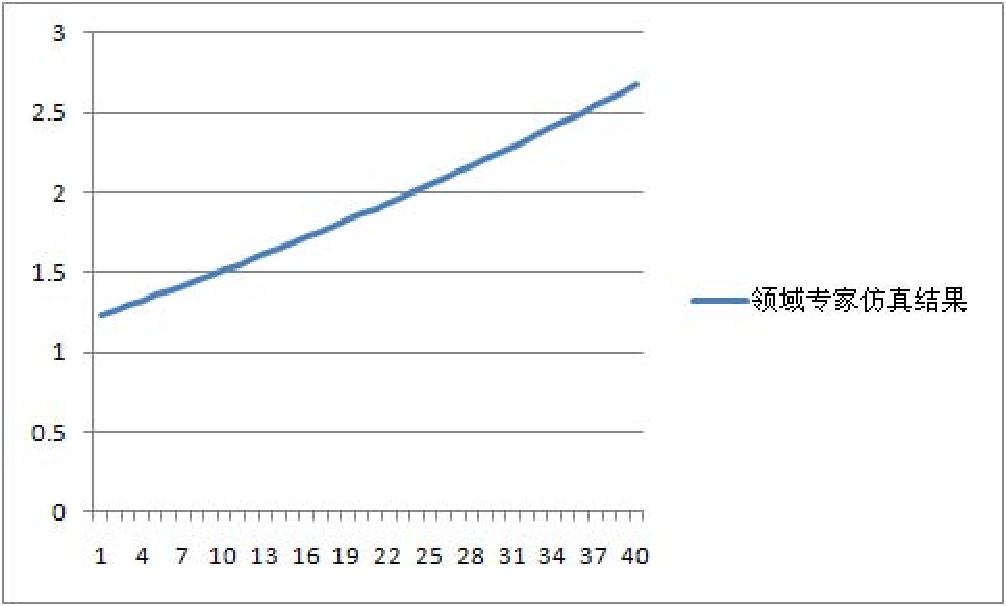
\includegraphics{improve3.pdf}}
  \caption{\small{\textbf{提升领域专家成就动机的仿真结果}}}
  % GNUPLOT: LaTeX picture
\setlength{\unitlength}{0.240900pt}
\ifx\plotpoint\undefined\newsavebox{\plotpoint}\fi
\begin{picture}(1500,900)(0,0)
\sbox{\plotpoint}{\rule[-0.200pt]{0.400pt}{0.400pt}}%
\put(131.0,82.0){\rule[-0.200pt]{4.818pt}{0.400pt}}
\put(111,82){\makebox(0,0)[r]{ 0}}
\put(1419.0,82.0){\rule[-0.200pt]{4.818pt}{0.400pt}}
\put(131.0,276.0){\rule[-0.200pt]{4.818pt}{0.400pt}}
\put(111,276){\makebox(0,0)[r]{ 1}}
\put(1419.0,276.0){\rule[-0.200pt]{4.818pt}{0.400pt}}
\put(131.0,471.0){\rule[-0.200pt]{4.818pt}{0.400pt}}
\put(111,471){\makebox(0,0)[r]{ 2}}
\put(1419.0,471.0){\rule[-0.200pt]{4.818pt}{0.400pt}}
\put(131.0,665.0){\rule[-0.200pt]{4.818pt}{0.400pt}}
\put(111,665){\makebox(0,0)[r]{ 3}}
\put(1419.0,665.0){\rule[-0.200pt]{4.818pt}{0.400pt}}
\put(131.0,82.0){\rule[-0.200pt]{0.400pt}{4.818pt}}
\put(131,41){\makebox(0,0){ 1}}
\put(131.0,839.0){\rule[-0.200pt]{0.400pt}{4.818pt}}
\put(198.0,82.0){\rule[-0.200pt]{0.400pt}{4.818pt}}
\put(198,41){\makebox(0,0){ 3}}
\put(198.0,839.0){\rule[-0.200pt]{0.400pt}{4.818pt}}
\put(265.0,82.0){\rule[-0.200pt]{0.400pt}{4.818pt}}
\put(265,41){\makebox(0,0){ 5}}
\put(265.0,839.0){\rule[-0.200pt]{0.400pt}{4.818pt}}
\put(332.0,82.0){\rule[-0.200pt]{0.400pt}{4.818pt}}
\put(332,41){\makebox(0,0){ 7}}
\put(332.0,839.0){\rule[-0.200pt]{0.400pt}{4.818pt}}
\put(399.0,82.0){\rule[-0.200pt]{0.400pt}{4.818pt}}
\put(399,41){\makebox(0,0){ 9}}
\put(399.0,839.0){\rule[-0.200pt]{0.400pt}{4.818pt}}
\put(466.0,82.0){\rule[-0.200pt]{0.400pt}{4.818pt}}
\put(466,41){\makebox(0,0){ 11}}
\put(466.0,839.0){\rule[-0.200pt]{0.400pt}{4.818pt}}
\put(533.0,82.0){\rule[-0.200pt]{0.400pt}{4.818pt}}
\put(533,41){\makebox(0,0){ 13}}
\put(533.0,839.0){\rule[-0.200pt]{0.400pt}{4.818pt}}
\put(601.0,82.0){\rule[-0.200pt]{0.400pt}{4.818pt}}
\put(601,41){\makebox(0,0){ 15}}
\put(601.0,839.0){\rule[-0.200pt]{0.400pt}{4.818pt}}
\put(668.0,82.0){\rule[-0.200pt]{0.400pt}{4.818pt}}
\put(668,41){\makebox(0,0){ 17}}
\put(668.0,839.0){\rule[-0.200pt]{0.400pt}{4.818pt}}
\put(735.0,82.0){\rule[-0.200pt]{0.400pt}{4.818pt}}
\put(735,41){\makebox(0,0){ 19}}
\put(735.0,839.0){\rule[-0.200pt]{0.400pt}{4.818pt}}
\put(802.0,82.0){\rule[-0.200pt]{0.400pt}{4.818pt}}
\put(802,41){\makebox(0,0){ 21}}
\put(802.0,839.0){\rule[-0.200pt]{0.400pt}{4.818pt}}
\put(869.0,82.0){\rule[-0.200pt]{0.400pt}{4.818pt}}
\put(869,41){\makebox(0,0){ 23}}
\put(869.0,839.0){\rule[-0.200pt]{0.400pt}{4.818pt}}
\put(936.0,82.0){\rule[-0.200pt]{0.400pt}{4.818pt}}
\put(936,41){\makebox(0,0){ 25}}
\put(936.0,839.0){\rule[-0.200pt]{0.400pt}{4.818pt}}
\put(1003.0,82.0){\rule[-0.200pt]{0.400pt}{4.818pt}}
\put(1003,41){\makebox(0,0){ 27}}
\put(1003.0,839.0){\rule[-0.200pt]{0.400pt}{4.818pt}}
\put(1070.0,82.0){\rule[-0.200pt]{0.400pt}{4.818pt}}
\put(1070,41){\makebox(0,0){ 29}}
\put(1070.0,839.0){\rule[-0.200pt]{0.400pt}{4.818pt}}
\put(1137.0,82.0){\rule[-0.200pt]{0.400pt}{4.818pt}}
\put(1137,41){\makebox(0,0){ 31}}
\put(1137.0,839.0){\rule[-0.200pt]{0.400pt}{4.818pt}}
\put(1204.0,82.0){\rule[-0.200pt]{0.400pt}{4.818pt}}
\put(1204,41){\makebox(0,0){ 33}}
\put(1204.0,839.0){\rule[-0.200pt]{0.400pt}{4.818pt}}
\put(1271.0,82.0){\rule[-0.200pt]{0.400pt}{4.818pt}}
\put(1271,41){\makebox(0,0){ 35}}
\put(1271.0,839.0){\rule[-0.200pt]{0.400pt}{4.818pt}}
\put(1338.0,82.0){\rule[-0.200pt]{0.400pt}{4.818pt}}
\put(1338,41){\makebox(0,0){ 37}}
\put(1338.0,839.0){\rule[-0.200pt]{0.400pt}{4.818pt}}
\put(1405.0,82.0){\rule[-0.200pt]{0.400pt}{4.818pt}}
\put(1405,41){\makebox(0,0){ 39}}
\put(1405.0,839.0){\rule[-0.200pt]{0.400pt}{4.818pt}}
\put(131.0,82.0){\rule[-0.200pt]{0.400pt}{187.179pt}}
\put(131.0,82.0){\rule[-0.200pt]{315.097pt}{0.400pt}}
\put(1439.0,82.0){\rule[-0.200pt]{0.400pt}{187.179pt}}
\put(131.0,859.0){\rule[-0.200pt]{315.097pt}{0.400pt}}
\put(30,470){\makebox(0,0){\rotatebox{90}{用户贡献}}}
\put(1279,819){\makebox(0,0)[r]{仿真数据}}
\put(1299.0,819.0){\rule[-0.200pt]{24.090pt}{0.400pt}}
\put(131,366){\usebox{\plotpoint}}
\multiput(131.00,364.92)(0.952,-0.495){33}{\rule{0.856pt}{0.119pt}}
\multiput(131.00,365.17)(32.224,-18.000){2}{\rule{0.428pt}{0.400pt}}
\multiput(165.00,346.92)(1.401,-0.492){21}{\rule{1.200pt}{0.119pt}}
\multiput(165.00,347.17)(30.509,-12.000){2}{\rule{0.600pt}{0.400pt}}
\multiput(198.00,334.93)(3.716,-0.477){7}{\rule{2.820pt}{0.115pt}}
\multiput(198.00,335.17)(28.147,-5.000){2}{\rule{1.410pt}{0.400pt}}
\multiput(232.00,329.93)(2.932,-0.482){9}{\rule{2.300pt}{0.116pt}}
\multiput(232.00,330.17)(28.226,-6.000){2}{\rule{1.150pt}{0.400pt}}
\multiput(265.00,323.93)(3.022,-0.482){9}{\rule{2.367pt}{0.116pt}}
\multiput(265.00,324.17)(29.088,-6.000){2}{\rule{1.183pt}{0.400pt}}
\multiput(299.00,317.94)(4.722,-0.468){5}{\rule{3.400pt}{0.113pt}}
\multiput(299.00,318.17)(25.943,-4.000){2}{\rule{1.700pt}{0.400pt}}
\put(332,313.17){\rule{6.900pt}{0.400pt}}
\multiput(332.00,314.17)(19.679,-2.000){2}{\rule{3.450pt}{0.400pt}}
\multiput(366.00,311.94)(4.722,-0.468){5}{\rule{3.400pt}{0.113pt}}
\multiput(366.00,312.17)(25.943,-4.000){2}{\rule{1.700pt}{0.400pt}}
\put(399,307.17){\rule{6.900pt}{0.400pt}}
\multiput(399.00,308.17)(19.679,-2.000){2}{\rule{3.450pt}{0.400pt}}
\put(433,305.17){\rule{6.700pt}{0.400pt}}
\multiput(433.00,306.17)(19.094,-2.000){2}{\rule{3.350pt}{0.400pt}}
\put(466,303.17){\rule{6.900pt}{0.400pt}}
\multiput(466.00,304.17)(19.679,-2.000){2}{\rule{3.450pt}{0.400pt}}
\put(500,301.67){\rule{7.950pt}{0.400pt}}
\multiput(500.00,302.17)(16.500,-1.000){2}{\rule{3.975pt}{0.400pt}}
\put(533,300.17){\rule{6.900pt}{0.400pt}}
\multiput(533.00,301.17)(19.679,-2.000){2}{\rule{3.450pt}{0.400pt}}
\put(567,298.17){\rule{6.900pt}{0.400pt}}
\multiput(567.00,299.17)(19.679,-2.000){2}{\rule{3.450pt}{0.400pt}}
\put(601,296.17){\rule{6.700pt}{0.400pt}}
\multiput(601.00,297.17)(19.094,-2.000){2}{\rule{3.350pt}{0.400pt}}
\put(634,294.17){\rule{6.900pt}{0.400pt}}
\multiput(634.00,295.17)(19.679,-2.000){2}{\rule{3.450pt}{0.400pt}}
\put(668,292.17){\rule{6.700pt}{0.400pt}}
\multiput(668.00,293.17)(19.094,-2.000){2}{\rule{3.350pt}{0.400pt}}
\put(735,290.17){\rule{6.700pt}{0.400pt}}
\multiput(735.00,291.17)(19.094,-2.000){2}{\rule{3.350pt}{0.400pt}}
\put(768,288.17){\rule{6.900pt}{0.400pt}}
\multiput(768.00,289.17)(19.679,-2.000){2}{\rule{3.450pt}{0.400pt}}
\put(701.0,292.0){\rule[-0.200pt]{8.191pt}{0.400pt}}
\put(835,286.17){\rule{6.900pt}{0.400pt}}
\multiput(835.00,287.17)(19.679,-2.000){2}{\rule{3.450pt}{0.400pt}}
\put(802.0,288.0){\rule[-0.200pt]{7.950pt}{0.400pt}}
\put(902,284.17){\rule{6.900pt}{0.400pt}}
\multiput(902.00,285.17)(19.679,-2.000){2}{\rule{3.450pt}{0.400pt}}
\put(869.0,286.0){\rule[-0.200pt]{7.950pt}{0.400pt}}
\put(969,282.17){\rule{6.900pt}{0.400pt}}
\multiput(969.00,283.17)(19.679,-2.000){2}{\rule{3.450pt}{0.400pt}}
\put(936.0,284.0){\rule[-0.200pt]{7.950pt}{0.400pt}}
\put(1037,280.17){\rule{6.700pt}{0.400pt}}
\multiput(1037.00,281.17)(19.094,-2.000){2}{\rule{3.350pt}{0.400pt}}
\put(1003.0,282.0){\rule[-0.200pt]{8.191pt}{0.400pt}}
\put(1104,278.17){\rule{6.700pt}{0.400pt}}
\multiput(1104.00,279.17)(19.094,-2.000){2}{\rule{3.350pt}{0.400pt}}
\put(1070.0,280.0){\rule[-0.200pt]{8.191pt}{0.400pt}}
\put(1171,276.17){\rule{6.700pt}{0.400pt}}
\multiput(1171.00,277.17)(19.094,-2.000){2}{\rule{3.350pt}{0.400pt}}
\put(1137.0,278.0){\rule[-0.200pt]{8.191pt}{0.400pt}}
\put(1271,274.17){\rule{6.900pt}{0.400pt}}
\multiput(1271.00,275.17)(19.679,-2.000){2}{\rule{3.450pt}{0.400pt}}
\put(1204.0,276.0){\rule[-0.200pt]{16.140pt}{0.400pt}}
\put(1372,272.17){\rule{6.700pt}{0.400pt}}
\multiput(1372.00,273.17)(19.094,-2.000){2}{\rule{3.350pt}{0.400pt}}
\put(1305.0,274.0){\rule[-0.200pt]{16.140pt}{0.400pt}}
\put(1405.0,272.0){\rule[-0.200pt]{8.191pt}{0.400pt}}
\put(1279,768){\makebox(0,0)[r]{改进数据}}
\put(1299.0,768.0){\rule[-0.200pt]{24.090pt}{0.400pt}}
\put(131,379){\usebox{\plotpoint}}
\multiput(131.00,379.59)(3.022,0.482){9}{\rule{2.367pt}{0.116pt}}
\multiput(131.00,378.17)(29.088,6.000){2}{\rule{1.183pt}{0.400pt}}
\multiput(165.00,385.59)(2.932,0.482){9}{\rule{2.300pt}{0.116pt}}
\multiput(165.00,384.17)(28.226,6.000){2}{\rule{1.150pt}{0.400pt}}
\multiput(198.00,391.59)(3.022,0.482){9}{\rule{2.367pt}{0.116pt}}
\multiput(198.00,390.17)(29.088,6.000){2}{\rule{1.183pt}{0.400pt}}
\multiput(265.00,397.61)(7.383,0.447){3}{\rule{4.633pt}{0.108pt}}
\multiput(265.00,396.17)(24.383,3.000){2}{\rule{2.317pt}{0.400pt}}
\multiput(299.00,400.59)(2.932,0.482){9}{\rule{2.300pt}{0.116pt}}
\multiput(299.00,399.17)(28.226,6.000){2}{\rule{1.150pt}{0.400pt}}
\multiput(332.00,406.59)(2.211,0.488){13}{\rule{1.800pt}{0.117pt}}
\multiput(332.00,405.17)(30.264,8.000){2}{\rule{0.900pt}{0.400pt}}
\multiput(366.00,414.61)(7.160,0.447){3}{\rule{4.500pt}{0.108pt}}
\multiput(366.00,413.17)(23.660,3.000){2}{\rule{2.250pt}{0.400pt}}
\put(399,417.17){\rule{6.900pt}{0.400pt}}
\multiput(399.00,416.17)(19.679,2.000){2}{\rule{3.450pt}{0.400pt}}
\multiput(433.00,419.61)(7.160,0.447){3}{\rule{4.500pt}{0.108pt}}
\multiput(433.00,418.17)(23.660,3.000){2}{\rule{2.250pt}{0.400pt}}
\multiput(466.00,422.59)(3.022,0.482){9}{\rule{2.367pt}{0.116pt}}
\multiput(466.00,421.17)(29.088,6.000){2}{\rule{1.183pt}{0.400pt}}
\put(500,427.67){\rule{7.950pt}{0.400pt}}
\multiput(500.00,427.17)(16.500,1.000){2}{\rule{3.975pt}{0.400pt}}
\multiput(533.00,429.58)(1.329,0.493){23}{\rule{1.146pt}{0.119pt}}
\multiput(533.00,428.17)(31.621,13.000){2}{\rule{0.573pt}{0.400pt}}
\multiput(567.00,442.59)(3.022,0.482){9}{\rule{2.367pt}{0.116pt}}
\multiput(567.00,441.17)(29.088,6.000){2}{\rule{1.183pt}{0.400pt}}
\multiput(601.00,448.59)(2.476,0.485){11}{\rule{1.986pt}{0.117pt}}
\multiput(601.00,447.17)(28.879,7.000){2}{\rule{0.993pt}{0.400pt}}
\multiput(634.00,455.58)(1.009,0.495){31}{\rule{0.900pt}{0.119pt}}
\multiput(634.00,454.17)(32.132,17.000){2}{\rule{0.450pt}{0.400pt}}
\multiput(668.00,472.59)(1.893,0.489){15}{\rule{1.567pt}{0.118pt}}
\multiput(668.00,471.17)(29.748,9.000){2}{\rule{0.783pt}{0.400pt}}
\multiput(701.00,481.58)(1.746,0.491){17}{\rule{1.460pt}{0.118pt}}
\multiput(701.00,480.17)(30.970,10.000){2}{\rule{0.730pt}{0.400pt}}
\multiput(735.00,491.60)(4.722,0.468){5}{\rule{3.400pt}{0.113pt}}
\multiput(735.00,490.17)(25.943,4.000){2}{\rule{1.700pt}{0.400pt}}
\multiput(768.00,495.61)(7.383,0.447){3}{\rule{4.633pt}{0.108pt}}
\multiput(768.00,494.17)(24.383,3.000){2}{\rule{2.317pt}{0.400pt}}
\multiput(802.00,498.59)(2.145,0.488){13}{\rule{1.750pt}{0.117pt}}
\multiput(802.00,497.17)(29.368,8.000){2}{\rule{0.875pt}{0.400pt}}
\multiput(835.00,506.59)(2.211,0.488){13}{\rule{1.800pt}{0.117pt}}
\multiput(835.00,505.17)(30.264,8.000){2}{\rule{0.900pt}{0.400pt}}
\multiput(869.00,514.58)(1.041,0.494){29}{\rule{0.925pt}{0.119pt}}
\multiput(869.00,513.17)(31.080,16.000){2}{\rule{0.463pt}{0.400pt}}
\multiput(902.00,530.59)(3.716,0.477){7}{\rule{2.820pt}{0.115pt}}
\multiput(902.00,529.17)(28.147,5.000){2}{\rule{1.410pt}{0.400pt}}
\multiput(936.00,535.59)(2.145,0.488){13}{\rule{1.750pt}{0.117pt}}
\multiput(936.00,534.17)(29.368,8.000){2}{\rule{0.875pt}{0.400pt}}
\multiput(969.00,543.58)(1.581,0.492){19}{\rule{1.336pt}{0.118pt}}
\multiput(969.00,542.17)(31.226,11.000){2}{\rule{0.668pt}{0.400pt}}
\multiput(1003.00,554.59)(2.211,0.488){13}{\rule{1.800pt}{0.117pt}}
\multiput(1003.00,553.17)(30.264,8.000){2}{\rule{0.900pt}{0.400pt}}
\multiput(1037.00,562.59)(2.476,0.485){11}{\rule{1.986pt}{0.117pt}}
\multiput(1037.00,561.17)(28.879,7.000){2}{\rule{0.993pt}{0.400pt}}
\multiput(1070.00,569.59)(2.211,0.488){13}{\rule{1.800pt}{0.117pt}}
\multiput(1070.00,568.17)(30.264,8.000){2}{\rule{0.900pt}{0.400pt}}
\multiput(1104.00,577.59)(2.145,0.488){13}{\rule{1.750pt}{0.117pt}}
\multiput(1104.00,576.17)(29.368,8.000){2}{\rule{0.875pt}{0.400pt}}
\multiput(1137.00,585.59)(2.211,0.488){13}{\rule{1.800pt}{0.117pt}}
\multiput(1137.00,584.17)(30.264,8.000){2}{\rule{0.900pt}{0.400pt}}
\multiput(1171.00,593.59)(2.145,0.488){13}{\rule{1.750pt}{0.117pt}}
\multiput(1171.00,592.17)(29.368,8.000){2}{\rule{0.875pt}{0.400pt}}
\multiput(1204.00,601.59)(2.211,0.488){13}{\rule{1.800pt}{0.117pt}}
\multiput(1204.00,600.17)(30.264,8.000){2}{\rule{0.900pt}{0.400pt}}
\multiput(1238.00,609.59)(1.893,0.489){15}{\rule{1.567pt}{0.118pt}}
\multiput(1238.00,608.17)(29.748,9.000){2}{\rule{0.783pt}{0.400pt}}
\multiput(1271.00,618.59)(2.211,0.488){13}{\rule{1.800pt}{0.117pt}}
\multiput(1271.00,617.17)(30.264,8.000){2}{\rule{0.900pt}{0.400pt}}
\multiput(1305.00,626.59)(2.145,0.488){13}{\rule{1.750pt}{0.117pt}}
\multiput(1305.00,625.17)(29.368,8.000){2}{\rule{0.875pt}{0.400pt}}
\multiput(1338.00,634.59)(1.951,0.489){15}{\rule{1.611pt}{0.118pt}}
\multiput(1338.00,633.17)(30.656,9.000){2}{\rule{0.806pt}{0.400pt}}
\multiput(1372.00,643.59)(2.145,0.488){13}{\rule{1.750pt}{0.117pt}}
\multiput(1372.00,642.17)(29.368,8.000){2}{\rule{0.875pt}{0.400pt}}
\multiput(1405.00,651.59)(1.951,0.489){15}{\rule{1.611pt}{0.118pt}}
\multiput(1405.00,650.17)(30.656,9.000){2}{\rule{0.806pt}{0.400pt}}
\put(131,379){\makebox(0,0){$+$}}
\put(165,385){\makebox(0,0){$+$}}
\put(198,391){\makebox(0,0){$+$}}
\put(232,397){\makebox(0,0){$+$}}
\put(265,397){\makebox(0,0){$+$}}
\put(299,400){\makebox(0,0){$+$}}
\put(332,406){\makebox(0,0){$+$}}
\put(366,414){\makebox(0,0){$+$}}
\put(399,417){\makebox(0,0){$+$}}
\put(433,419){\makebox(0,0){$+$}}
\put(466,422){\makebox(0,0){$+$}}
\put(500,428){\makebox(0,0){$+$}}
\put(533,429){\makebox(0,0){$+$}}
\put(567,442){\makebox(0,0){$+$}}
\put(601,448){\makebox(0,0){$+$}}
\put(634,455){\makebox(0,0){$+$}}
\put(668,472){\makebox(0,0){$+$}}
\put(701,481){\makebox(0,0){$+$}}
\put(735,491){\makebox(0,0){$+$}}
\put(768,495){\makebox(0,0){$+$}}
\put(802,498){\makebox(0,0){$+$}}
\put(835,506){\makebox(0,0){$+$}}
\put(869,514){\makebox(0,0){$+$}}
\put(902,530){\makebox(0,0){$+$}}
\put(936,535){\makebox(0,0){$+$}}
\put(969,543){\makebox(0,0){$+$}}
\put(1003,554){\makebox(0,0){$+$}}
\put(1037,562){\makebox(0,0){$+$}}
\put(1070,569){\makebox(0,0){$+$}}
\put(1104,577){\makebox(0,0){$+$}}
\put(1137,585){\makebox(0,0){$+$}}
\put(1171,593){\makebox(0,0){$+$}}
\put(1204,601){\makebox(0,0){$+$}}
\put(1238,609){\makebox(0,0){$+$}}
\put(1271,618){\makebox(0,0){$+$}}
\put(1305,626){\makebox(0,0){$+$}}
\put(1338,634){\makebox(0,0){$+$}}
\put(1372,643){\makebox(0,0){$+$}}
\put(1405,651){\makebox(0,0){$+$}}
\put(1439,660){\makebox(0,0){$+$}}
\put(1349,768){\makebox(0,0){$+$}}
\put(232.0,397.0){\rule[-0.200pt]{7.950pt}{0.400pt}}
\put(131.0,82.0){\rule[-0.200pt]{0.400pt}{187.179pt}}
\put(131.0,82.0){\rule[-0.200pt]{315.097pt}{0.400pt}}
\put(1439.0,82.0){\rule[-0.200pt]{0.400pt}{187.179pt}}
\put(131.0,859.0){\rule[-0.200pt]{315.097pt}{0.400pt}}
\end{picture}
 
  \label{fig:improve3}
\end{figure}

领域专家用户具有和领导者相似的协同模式和个人能力,但是其容易“自满”的
特点限制了其发挥自身的最大能力。如果社区能够采取措施将领域专家转化为领
导者,那么对于社区的发展将是大有裨益的。首先,应该加强领域专家用户的成
就期待感,让他们认识到仅仅完成一两个条目的撰写还远远不是成功的终点,只
有唤起他们更大的成功欲望,才能有效地克服“自满”情绪。同时,社区给与这
类用户充分的支持和鼓励,这样有助于调整内部动机各个因素间的比率,降低成
就需求的比重,使那些具有正反馈关系的动机占据主要地位,最大限度地提升领
域专家用户的参与水平。

\subsection{内容贡献者}

内容贡献者是社区的中坚力量。个体层面的动机和群体层面的动机都会影响他们
参与知识协同的程度。内容贡献者的月人均贡献度的变化很平缓,但是仍然可以
看到加速上升的趋势,这意味着正反馈对协同水平起到了主要作用。同时,内容
贡献者的贡献度水平非常高,在所有用户群体中仅次于领导者用户。因此,这类
用户并不存在领域专家那种容易“自满”的特点。

尽管内容贡献者的贡献度呈现指数增长的特点,但是其增长速度非常缓慢。通过
对比其月度的总贡献和月度的正贡献可以发现:总贡献和正贡献的值非常接近,
就平均水平而言,正贡献与总贡献的差小于$10\%$,而二者最大的差值仅为
$18\%$。这意味着内容贡献者的工作水平非常高,大部分编辑内容都被其他协同
着接受而得以保留。因此内容贡献者所得到的负反馈实际上是非常少的。造成内
容贡献者贡献增长较慢的主要原因是其动机的初始值较低。只有在经历较长时间
后,正反馈的效应才能逐渐体现出来。内容贡献者同领导者用户不同,他们的动
机水平是在协同过程中不断获得正反馈得到的,而不是一开始就有很强的动机。
以下两个仿真验证了这一点。

图\ref{fig:improve5}是将所有的个体层次动机的初始值提升了$10\%$后的仿真结果。动机提升后个
体的贡献度有了一定的提高,同时随时间加速上升的趋势也要比提升前明显。这
个结果证明如果初始动机水平高,那么参与水平的提升速度也会提高。

\begin{figure}[!htb]
  \centering
%  \scalebox{0.65}{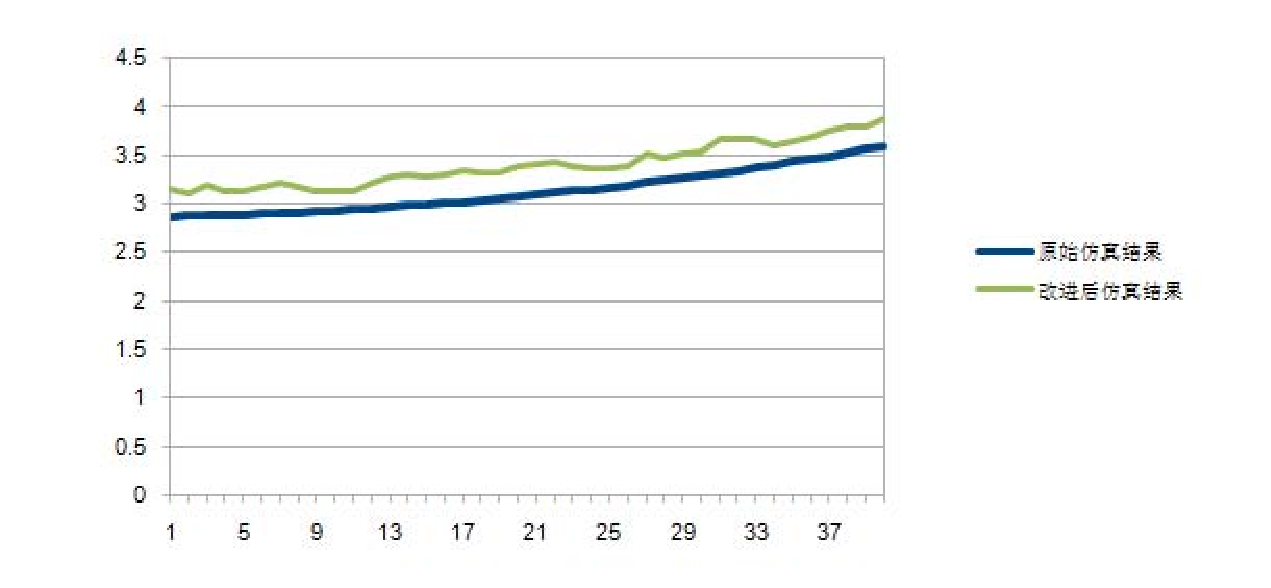
\includegraphics{improve5.pdf}}
  % GNUPLOT: LaTeX picture
\setlength{\unitlength}{0.240900pt}
\ifx\plotpoint\undefined\newsavebox{\plotpoint}\fi
\begin{picture}(1500,900)(0,0)
\sbox{\plotpoint}{\rule[-0.200pt]{0.400pt}{0.400pt}}%
\put(131.0,82.0){\rule[-0.200pt]{4.818pt}{0.400pt}}
\put(111,82){\makebox(0,0)[r]{ 0}}
\put(1419.0,82.0){\rule[-0.200pt]{4.818pt}{0.400pt}}
\put(131.0,237.0){\rule[-0.200pt]{4.818pt}{0.400pt}}
\put(111,237){\makebox(0,0)[r]{ 1}}
\put(1419.0,237.0){\rule[-0.200pt]{4.818pt}{0.400pt}}
\put(131.0,393.0){\rule[-0.200pt]{4.818pt}{0.400pt}}
\put(111,393){\makebox(0,0)[r]{ 2}}
\put(1419.0,393.0){\rule[-0.200pt]{4.818pt}{0.400pt}}
\put(131.0,548.0){\rule[-0.200pt]{4.818pt}{0.400pt}}
\put(111,548){\makebox(0,0)[r]{ 3}}
\put(1419.0,548.0){\rule[-0.200pt]{4.818pt}{0.400pt}}
\put(131.0,704.0){\rule[-0.200pt]{4.818pt}{0.400pt}}
\put(111,704){\makebox(0,0)[r]{ 4}}
\put(1419.0,704.0){\rule[-0.200pt]{4.818pt}{0.400pt}}
\put(131.0,82.0){\rule[-0.200pt]{0.400pt}{4.818pt}}
\put(131,41){\makebox(0,0){ 1}}
\put(131.0,839.0){\rule[-0.200pt]{0.400pt}{4.818pt}}
\put(198.0,82.0){\rule[-0.200pt]{0.400pt}{4.818pt}}
\put(198,41){\makebox(0,0){ 3}}
\put(198.0,839.0){\rule[-0.200pt]{0.400pt}{4.818pt}}
\put(265.0,82.0){\rule[-0.200pt]{0.400pt}{4.818pt}}
\put(265,41){\makebox(0,0){ 5}}
\put(265.0,839.0){\rule[-0.200pt]{0.400pt}{4.818pt}}
\put(332.0,82.0){\rule[-0.200pt]{0.400pt}{4.818pt}}
\put(332,41){\makebox(0,0){ 7}}
\put(332.0,839.0){\rule[-0.200pt]{0.400pt}{4.818pt}}
\put(399.0,82.0){\rule[-0.200pt]{0.400pt}{4.818pt}}
\put(399,41){\makebox(0,0){ 9}}
\put(399.0,839.0){\rule[-0.200pt]{0.400pt}{4.818pt}}
\put(466.0,82.0){\rule[-0.200pt]{0.400pt}{4.818pt}}
\put(466,41){\makebox(0,0){ 11}}
\put(466.0,839.0){\rule[-0.200pt]{0.400pt}{4.818pt}}
\put(533.0,82.0){\rule[-0.200pt]{0.400pt}{4.818pt}}
\put(533,41){\makebox(0,0){ 13}}
\put(533.0,839.0){\rule[-0.200pt]{0.400pt}{4.818pt}}
\put(601.0,82.0){\rule[-0.200pt]{0.400pt}{4.818pt}}
\put(601,41){\makebox(0,0){ 15}}
\put(601.0,839.0){\rule[-0.200pt]{0.400pt}{4.818pt}}
\put(668.0,82.0){\rule[-0.200pt]{0.400pt}{4.818pt}}
\put(668,41){\makebox(0,0){ 17}}
\put(668.0,839.0){\rule[-0.200pt]{0.400pt}{4.818pt}}
\put(735.0,82.0){\rule[-0.200pt]{0.400pt}{4.818pt}}
\put(735,41){\makebox(0,0){ 19}}
\put(735.0,839.0){\rule[-0.200pt]{0.400pt}{4.818pt}}
\put(802.0,82.0){\rule[-0.200pt]{0.400pt}{4.818pt}}
\put(802,41){\makebox(0,0){ 21}}
\put(802.0,839.0){\rule[-0.200pt]{0.400pt}{4.818pt}}
\put(869.0,82.0){\rule[-0.200pt]{0.400pt}{4.818pt}}
\put(869,41){\makebox(0,0){ 23}}
\put(869.0,839.0){\rule[-0.200pt]{0.400pt}{4.818pt}}
\put(936.0,82.0){\rule[-0.200pt]{0.400pt}{4.818pt}}
\put(936,41){\makebox(0,0){ 25}}
\put(936.0,839.0){\rule[-0.200pt]{0.400pt}{4.818pt}}
\put(1003.0,82.0){\rule[-0.200pt]{0.400pt}{4.818pt}}
\put(1003,41){\makebox(0,0){ 27}}
\put(1003.0,839.0){\rule[-0.200pt]{0.400pt}{4.818pt}}
\put(1070.0,82.0){\rule[-0.200pt]{0.400pt}{4.818pt}}
\put(1070,41){\makebox(0,0){ 29}}
\put(1070.0,839.0){\rule[-0.200pt]{0.400pt}{4.818pt}}
\put(1137.0,82.0){\rule[-0.200pt]{0.400pt}{4.818pt}}
\put(1137,41){\makebox(0,0){ 31}}
\put(1137.0,839.0){\rule[-0.200pt]{0.400pt}{4.818pt}}
\put(1204.0,82.0){\rule[-0.200pt]{0.400pt}{4.818pt}}
\put(1204,41){\makebox(0,0){ 33}}
\put(1204.0,839.0){\rule[-0.200pt]{0.400pt}{4.818pt}}
\put(1271.0,82.0){\rule[-0.200pt]{0.400pt}{4.818pt}}
\put(1271,41){\makebox(0,0){ 35}}
\put(1271.0,839.0){\rule[-0.200pt]{0.400pt}{4.818pt}}
\put(1338.0,82.0){\rule[-0.200pt]{0.400pt}{4.818pt}}
\put(1338,41){\makebox(0,0){ 37}}
\put(1338.0,839.0){\rule[-0.200pt]{0.400pt}{4.818pt}}
\put(1405.0,82.0){\rule[-0.200pt]{0.400pt}{4.818pt}}
\put(1405,41){\makebox(0,0){ 39}}
\put(1405.0,839.0){\rule[-0.200pt]{0.400pt}{4.818pt}}
\put(131.0,82.0){\rule[-0.200pt]{0.400pt}{187.179pt}}
\put(131.0,82.0){\rule[-0.200pt]{315.097pt}{0.400pt}}
\put(1439.0,82.0){\rule[-0.200pt]{0.400pt}{187.179pt}}
\put(131.0,859.0){\rule[-0.200pt]{315.097pt}{0.400pt}}
\put(30,470){\makebox(0,0){\rotatebox{90}{用户贡献}}}
\put(785,-10){\makebox(0,0){月度}}
\put(1279,819){\makebox(0,0)[r]{仿真数据}}
\put(1299.0,819.0){\rule[-0.200pt]{24.090pt}{0.400pt}}
\put(1439,640){\usebox{\plotpoint}}
\multiput(1427.29,638.93)(-3.716,-0.477){7}{\rule{2.820pt}{0.115pt}}
\multiput(1433.15,639.17)(-28.147,-5.000){2}{\rule{1.410pt}{0.400pt}}
\multiput(1393.63,633.93)(-3.604,-0.477){7}{\rule{2.740pt}{0.115pt}}
\multiput(1399.31,634.17)(-27.313,-5.000){2}{\rule{1.370pt}{0.400pt}}
\multiput(1360.29,628.93)(-3.716,-0.477){7}{\rule{2.820pt}{0.115pt}}
\multiput(1366.15,629.17)(-28.147,-5.000){2}{\rule{1.410pt}{0.400pt}}
\multiput(1326.63,623.93)(-3.604,-0.477){7}{\rule{2.740pt}{0.115pt}}
\multiput(1332.31,624.17)(-27.313,-5.000){2}{\rule{1.370pt}{0.400pt}}
\multiput(1293.29,618.93)(-3.716,-0.477){7}{\rule{2.820pt}{0.115pt}}
\multiput(1299.15,619.17)(-28.147,-5.000){2}{\rule{1.410pt}{0.400pt}}
\multiput(1256.89,613.94)(-4.722,-0.468){5}{\rule{3.400pt}{0.113pt}}
\multiput(1263.94,614.17)(-25.943,-4.000){2}{\rule{1.700pt}{0.400pt}}
\multiput(1226.29,609.93)(-3.716,-0.477){7}{\rule{2.820pt}{0.115pt}}
\multiput(1232.15,610.17)(-28.147,-5.000){2}{\rule{1.410pt}{0.400pt}}
\multiput(1189.89,604.94)(-4.722,-0.468){5}{\rule{3.400pt}{0.113pt}}
\multiput(1196.94,605.17)(-25.943,-4.000){2}{\rule{1.700pt}{0.400pt}}
\multiput(1156.47,600.94)(-4.868,-0.468){5}{\rule{3.500pt}{0.113pt}}
\multiput(1163.74,601.17)(-26.736,-4.000){2}{\rule{1.750pt}{0.400pt}}
\multiput(1125.63,596.93)(-3.604,-0.477){7}{\rule{2.740pt}{0.115pt}}
\multiput(1131.31,597.17)(-27.313,-5.000){2}{\rule{1.370pt}{0.400pt}}
\multiput(1089.47,591.94)(-4.868,-0.468){5}{\rule{3.500pt}{0.113pt}}
\multiput(1096.74,592.17)(-26.736,-4.000){2}{\rule{1.750pt}{0.400pt}}
\multiput(1051.32,587.95)(-7.160,-0.447){3}{\rule{4.500pt}{0.108pt}}
\multiput(1060.66,588.17)(-23.660,-3.000){2}{\rule{2.250pt}{0.400pt}}
\multiput(1022.47,584.94)(-4.868,-0.468){5}{\rule{3.500pt}{0.113pt}}
\multiput(1029.74,585.17)(-26.736,-4.000){2}{\rule{1.750pt}{0.400pt}}
\multiput(988.47,580.94)(-4.868,-0.468){5}{\rule{3.500pt}{0.113pt}}
\multiput(995.74,581.17)(-26.736,-4.000){2}{\rule{1.750pt}{0.400pt}}
\multiput(950.32,576.95)(-7.160,-0.447){3}{\rule{4.500pt}{0.108pt}}
\multiput(959.66,577.17)(-23.660,-3.000){2}{\rule{2.250pt}{0.400pt}}
\multiput(921.47,573.94)(-4.868,-0.468){5}{\rule{3.500pt}{0.113pt}}
\multiput(928.74,574.17)(-26.736,-4.000){2}{\rule{1.750pt}{0.400pt}}
\multiput(883.32,569.95)(-7.160,-0.447){3}{\rule{4.500pt}{0.108pt}}
\multiput(892.66,570.17)(-23.660,-3.000){2}{\rule{2.250pt}{0.400pt}}
\multiput(849.77,566.95)(-7.383,-0.447){3}{\rule{4.633pt}{0.108pt}}
\multiput(859.38,567.17)(-24.383,-3.000){2}{\rule{2.317pt}{0.400pt}}
\multiput(816.32,563.95)(-7.160,-0.447){3}{\rule{4.500pt}{0.108pt}}
\multiput(825.66,564.17)(-23.660,-3.000){2}{\rule{2.250pt}{0.400pt}}
\multiput(782.77,560.95)(-7.383,-0.447){3}{\rule{4.633pt}{0.108pt}}
\multiput(792.38,561.17)(-24.383,-3.000){2}{\rule{2.317pt}{0.400pt}}
\put(735,557.17){\rule{6.700pt}{0.400pt}}
\multiput(754.09,558.17)(-19.094,-2.000){2}{\rule{3.350pt}{0.400pt}}
\multiput(715.77,555.95)(-7.383,-0.447){3}{\rule{4.633pt}{0.108pt}}
\multiput(725.38,556.17)(-24.383,-3.000){2}{\rule{2.317pt}{0.400pt}}
\multiput(682.32,552.95)(-7.160,-0.447){3}{\rule{4.500pt}{0.108pt}}
\multiput(691.66,553.17)(-23.660,-3.000){2}{\rule{2.250pt}{0.400pt}}
\put(634,549.17){\rule{6.900pt}{0.400pt}}
\multiput(653.68,550.17)(-19.679,-2.000){2}{\rule{3.450pt}{0.400pt}}
\put(601,547.17){\rule{6.700pt}{0.400pt}}
\multiput(620.09,548.17)(-19.094,-2.000){2}{\rule{3.350pt}{0.400pt}}
\put(567,545.17){\rule{6.900pt}{0.400pt}}
\multiput(586.68,546.17)(-19.679,-2.000){2}{\rule{3.450pt}{0.400pt}}
\put(533,543.17){\rule{6.900pt}{0.400pt}}
\multiput(552.68,544.17)(-19.679,-2.000){2}{\rule{3.450pt}{0.400pt}}
\put(500,541.17){\rule{6.700pt}{0.400pt}}
\multiput(519.09,542.17)(-19.094,-2.000){2}{\rule{3.350pt}{0.400pt}}
\put(466,539.17){\rule{6.900pt}{0.400pt}}
\multiput(485.68,540.17)(-19.679,-2.000){2}{\rule{3.450pt}{0.400pt}}
\put(433,537.17){\rule{6.700pt}{0.400pt}}
\multiput(452.09,538.17)(-19.094,-2.000){2}{\rule{3.350pt}{0.400pt}}
\put(399,535.67){\rule{8.191pt}{0.400pt}}
\multiput(416.00,536.17)(-17.000,-1.000){2}{\rule{4.095pt}{0.400pt}}
\put(366,534.67){\rule{7.950pt}{0.400pt}}
\multiput(382.50,535.17)(-16.500,-1.000){2}{\rule{3.975pt}{0.400pt}}
\put(332,533.17){\rule{6.900pt}{0.400pt}}
\multiput(351.68,534.17)(-19.679,-2.000){2}{\rule{3.450pt}{0.400pt}}
\put(299,531.67){\rule{7.950pt}{0.400pt}}
\multiput(315.50,532.17)(-16.500,-1.000){2}{\rule{3.975pt}{0.400pt}}
\put(265,530.67){\rule{8.191pt}{0.400pt}}
\multiput(282.00,531.17)(-17.000,-1.000){2}{\rule{4.095pt}{0.400pt}}
\put(232,529.67){\rule{7.950pt}{0.400pt}}
\multiput(248.50,530.17)(-16.500,-1.000){2}{\rule{3.975pt}{0.400pt}}
\put(165,528.67){\rule{7.950pt}{0.400pt}}
\multiput(181.50,529.17)(-16.500,-1.000){2}{\rule{3.975pt}{0.400pt}}
\put(198.0,530.0){\rule[-0.200pt]{8.191pt}{0.400pt}}
\put(131.0,529.0){\rule[-0.200pt]{8.191pt}{0.400pt}}
\put(1279,768){\makebox(0,0)[r]{改进数据}}
\put(1299.0,768.0){\rule[-0.200pt]{24.090pt}{0.400pt}}
\put(1439,659){\usebox{\plotpoint}}
\multiput(1432.31,657.93)(-1.951,-0.489){15}{\rule{1.611pt}{0.118pt}}
\multiput(1435.66,658.17)(-30.656,-9.000){2}{\rule{0.806pt}{0.400pt}}
\put(1372,648.17){\rule{6.700pt}{0.400pt}}
\multiput(1391.09,649.17)(-19.094,-2.000){2}{\rule{3.350pt}{0.400pt}}
\multiput(1364.53,646.93)(-2.211,-0.488){13}{\rule{1.800pt}{0.117pt}}
\multiput(1368.26,647.17)(-30.264,-8.000){2}{\rule{0.900pt}{0.400pt}}
\multiput(1319.32,638.95)(-7.160,-0.447){3}{\rule{4.500pt}{0.108pt}}
\multiput(1328.66,639.17)(-23.660,-3.000){2}{\rule{2.250pt}{0.400pt}}
\put(1271,635.67){\rule{8.191pt}{0.400pt}}
\multiput(1288.00,636.17)(-17.000,-1.000){2}{\rule{4.095pt}{0.400pt}}
\multiput(1256.89,634.94)(-4.722,-0.468){5}{\rule{3.400pt}{0.113pt}}
\multiput(1263.94,635.17)(-25.943,-4.000){2}{\rule{1.700pt}{0.400pt}}
\put(1204,630.17){\rule{6.900pt}{0.400pt}}
\multiput(1223.68,631.17)(-19.679,-2.000){2}{\rule{3.450pt}{0.400pt}}
\multiput(1198.60,628.92)(-1.534,-0.492){19}{\rule{1.300pt}{0.118pt}}
\multiput(1201.30,629.17)(-30.302,-11.000){2}{\rule{0.650pt}{0.400pt}}
\multiput(1122.89,617.94)(-4.722,-0.468){5}{\rule{3.400pt}{0.113pt}}
\multiput(1129.94,618.17)(-25.943,-4.000){2}{\rule{1.700pt}{0.400pt}}
\put(1137.0,619.0){\rule[-0.200pt]{8.191pt}{0.400pt}}
\multiput(1058.63,613.93)(-3.604,-0.477){7}{\rule{2.740pt}{0.115pt}}
\multiput(1064.31,614.17)(-27.313,-5.000){2}{\rule{1.370pt}{0.400pt}}
\multiput(1025.29,608.93)(-3.716,-0.477){7}{\rule{2.820pt}{0.115pt}}
\multiput(1031.15,609.17)(-28.147,-5.000){2}{\rule{1.410pt}{0.400pt}}
\put(969,603.17){\rule{6.900pt}{0.400pt}}
\multiput(988.68,604.17)(-19.679,-2.000){2}{\rule{3.450pt}{0.400pt}}
\multiput(963.60,601.92)(-1.534,-0.492){19}{\rule{1.300pt}{0.118pt}}
\multiput(966.30,602.17)(-30.302,-11.000){2}{\rule{0.650pt}{0.400pt}}
\put(902,590.67){\rule{8.191pt}{0.400pt}}
\multiput(919.00,591.17)(-17.000,-1.000){2}{\rule{4.095pt}{0.400pt}}
\multiput(883.32,589.95)(-7.160,-0.447){3}{\rule{4.500pt}{0.108pt}}
\multiput(892.66,590.17)(-23.660,-3.000){2}{\rule{2.250pt}{0.400pt}}
\multiput(849.77,586.95)(-7.383,-0.447){3}{\rule{4.633pt}{0.108pt}}
\multiput(859.38,587.17)(-24.383,-3.000){2}{\rule{2.317pt}{0.400pt}}
\multiput(826.76,583.93)(-2.476,-0.485){11}{\rule{1.986pt}{0.117pt}}
\multiput(830.88,584.17)(-28.879,-7.000){2}{\rule{0.993pt}{0.400pt}}
\multiput(782.77,578.61)(-7.383,0.447){3}{\rule{4.633pt}{0.108pt}}
\multiput(792.38,577.17)(-24.383,3.000){2}{\rule{2.317pt}{0.400pt}}
\multiput(759.76,579.93)(-2.476,-0.485){11}{\rule{1.986pt}{0.117pt}}
\multiput(763.88,580.17)(-28.879,-7.000){2}{\rule{0.993pt}{0.400pt}}
\multiput(715.77,572.95)(-7.383,-0.447){3}{\rule{4.633pt}{0.108pt}}
\multiput(725.38,573.17)(-24.383,-3.000){2}{\rule{2.317pt}{0.400pt}}
\put(668,569.67){\rule{7.950pt}{0.400pt}}
\multiput(684.50,570.17)(-16.500,-1.000){2}{\rule{3.975pt}{0.400pt}}
\put(1070.0,615.0){\rule[-0.200pt]{8.191pt}{0.400pt}}
\multiput(586.47,568.94)(-4.868,-0.468){5}{\rule{3.500pt}{0.113pt}}
\multiput(593.74,569.17)(-26.736,-4.000){2}{\rule{1.750pt}{0.400pt}}
\put(533,566.17){\rule{6.900pt}{0.400pt}}
\multiput(552.68,565.17)(-19.679,2.000){2}{\rule{3.450pt}{0.400pt}}
\put(500,568.17){\rule{6.700pt}{0.400pt}}
\multiput(519.09,567.17)(-19.094,2.000){2}{\rule{3.350pt}{0.400pt}}
\multiput(485.47,568.94)(-4.868,-0.468){5}{\rule{3.500pt}{0.113pt}}
\multiput(492.74,569.17)(-26.736,-4.000){2}{\rule{1.750pt}{0.400pt}}
\put(433,565.67){\rule{7.950pt}{0.400pt}}
\multiput(449.50,565.17)(-16.500,1.000){2}{\rule{3.975pt}{0.400pt}}
\multiput(423.18,565.93)(-3.022,-0.482){9}{\rule{2.367pt}{0.116pt}}
\multiput(428.09,566.17)(-29.088,-6.000){2}{\rule{1.183pt}{0.400pt}}
\multiput(387.63,559.93)(-3.604,-0.477){7}{\rule{2.740pt}{0.115pt}}
\multiput(393.31,560.17)(-27.313,-5.000){2}{\rule{1.370pt}{0.400pt}}
\put(332,555.67){\rule{8.191pt}{0.400pt}}
\multiput(349.00,555.17)(-17.000,1.000){2}{\rule{4.095pt}{0.400pt}}
\multiput(313.32,555.95)(-7.160,-0.447){3}{\rule{4.500pt}{0.108pt}}
\multiput(322.66,556.17)(-23.660,-3.000){2}{\rule{2.250pt}{0.400pt}}
\multiput(291.53,552.93)(-2.211,-0.488){13}{\rule{1.800pt}{0.117pt}}
\multiput(295.26,553.17)(-30.264,-8.000){2}{\rule{0.900pt}{0.400pt}}
\multiput(246.32,546.61)(-7.160,0.447){3}{\rule{4.500pt}{0.108pt}}
\multiput(255.66,545.17)(-23.660,3.000){2}{\rule{2.250pt}{0.400pt}}
\multiput(224.53,547.93)(-2.211,-0.488){13}{\rule{1.800pt}{0.117pt}}
\multiput(228.26,548.17)(-30.264,-8.000){2}{\rule{0.900pt}{0.400pt}}
\multiput(179.32,539.95)(-7.160,-0.447){3}{\rule{4.500pt}{0.108pt}}
\multiput(188.66,540.17)(-23.660,-3.000){2}{\rule{2.250pt}{0.400pt}}
\multiput(156.52,536.93)(-2.552,-0.485){11}{\rule{2.043pt}{0.117pt}}
\multiput(160.76,537.17)(-29.760,-7.000){2}{\rule{1.021pt}{0.400pt}}
\put(1439,659){\makebox(0,0){$+$}}
\put(1405,650){\makebox(0,0){$+$}}
\put(1372,648){\makebox(0,0){$+$}}
\put(1338,640){\makebox(0,0){$+$}}
\put(1305,637){\makebox(0,0){$+$}}
\put(1271,636){\makebox(0,0){$+$}}
\put(1238,632){\makebox(0,0){$+$}}
\put(1204,630){\makebox(0,0){$+$}}
\put(1171,619){\makebox(0,0){$+$}}
\put(1137,619){\makebox(0,0){$+$}}
\put(1104,615){\makebox(0,0){$+$}}
\put(1070,615){\makebox(0,0){$+$}}
\put(1037,610){\makebox(0,0){$+$}}
\put(1003,605){\makebox(0,0){$+$}}
\put(969,603){\makebox(0,0){$+$}}
\put(936,592){\makebox(0,0){$+$}}
\put(902,591){\makebox(0,0){$+$}}
\put(869,588){\makebox(0,0){$+$}}
\put(835,585){\makebox(0,0){$+$}}
\put(802,578){\makebox(0,0){$+$}}
\put(768,581){\makebox(0,0){$+$}}
\put(735,574){\makebox(0,0){$+$}}
\put(701,571){\makebox(0,0){$+$}}
\put(668,570){\makebox(0,0){$+$}}
\put(634,570){\makebox(0,0){$+$}}
\put(601,570){\makebox(0,0){$+$}}
\put(567,566){\makebox(0,0){$+$}}
\put(533,568){\makebox(0,0){$+$}}
\put(500,570){\makebox(0,0){$+$}}
\put(466,566){\makebox(0,0){$+$}}
\put(433,567){\makebox(0,0){$+$}}
\put(399,561){\makebox(0,0){$+$}}
\put(366,556){\makebox(0,0){$+$}}
\put(332,557){\makebox(0,0){$+$}}
\put(299,554){\makebox(0,0){$+$}}
\put(265,546){\makebox(0,0){$+$}}
\put(232,549){\makebox(0,0){$+$}}
\put(198,541){\makebox(0,0){$+$}}
\put(165,538){\makebox(0,0){$+$}}
\put(131,531){\makebox(0,0){$+$}}
\put(1349,768){\makebox(0,0){$+$}}
\put(601.0,570.0){\rule[-0.200pt]{16.140pt}{0.400pt}}
\put(131.0,82.0){\rule[-0.200pt]{0.400pt}{187.179pt}}
\put(131.0,82.0){\rule[-0.200pt]{315.097pt}{0.400pt}}
\put(1439.0,82.0){\rule[-0.200pt]{0.400pt}{187.179pt}}
\put(131.0,859.0){\rule[-0.200pt]{315.097pt}{0.400pt}}
\end{picture}

 \caption{\small{\textbf{提升内容贡献者个体动机的仿真结果}}}
  \label{fig:improve5}
\end{figure}

图\ref{fig:improve6}是将所有的群体层次动机的初始值提升了$10\%$后的仿真结果。动机提升后个
体的贡献度同样有了一定的提高,同时随时间加速上升的趋势也要比提升前明显。
两个仿真的结果还表明,提升个体动机和人际间动机效果是一样
的。内容贡献者既重视在知识协同中获得心理上的满足感,同时也从与他人的互
动过程中获得良好的体验。

\begin{figure}[!htb]
  \centering
%  \scalebox{0.65}{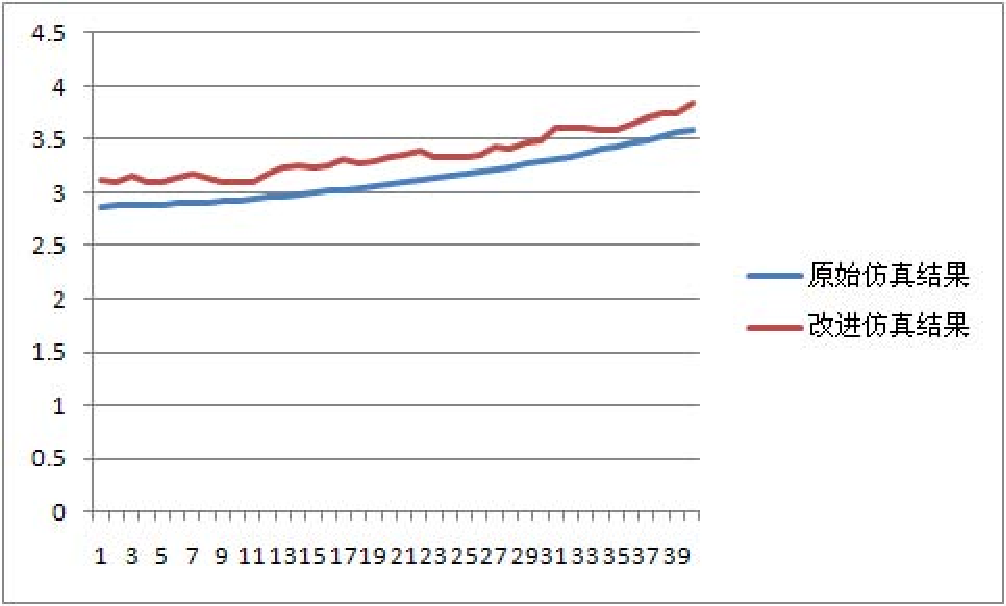
\includegraphics{improve6.pdf}}
  % GNUPLOT: LaTeX picture
\setlength{\unitlength}{0.240900pt}
\ifx\plotpoint\undefined\newsavebox{\plotpoint}\fi
\begin{picture}(1500,900)(0,0)
\sbox{\plotpoint}{\rule[-0.200pt]{0.400pt}{0.400pt}}%
\put(131.0,82.0){\rule[-0.200pt]{4.818pt}{0.400pt}}
\put(111,82){\makebox(0,0)[r]{ 0}}
\put(1419.0,82.0){\rule[-0.200pt]{4.818pt}{0.400pt}}
\put(131.0,237.0){\rule[-0.200pt]{4.818pt}{0.400pt}}
\put(111,237){\makebox(0,0)[r]{ 1}}
\put(1419.0,237.0){\rule[-0.200pt]{4.818pt}{0.400pt}}
\put(131.0,393.0){\rule[-0.200pt]{4.818pt}{0.400pt}}
\put(111,393){\makebox(0,0)[r]{ 2}}
\put(1419.0,393.0){\rule[-0.200pt]{4.818pt}{0.400pt}}
\put(131.0,548.0){\rule[-0.200pt]{4.818pt}{0.400pt}}
\put(111,548){\makebox(0,0)[r]{ 3}}
\put(1419.0,548.0){\rule[-0.200pt]{4.818pt}{0.400pt}}
\put(131.0,704.0){\rule[-0.200pt]{4.818pt}{0.400pt}}
\put(111,704){\makebox(0,0)[r]{ 4}}
\put(1419.0,704.0){\rule[-0.200pt]{4.818pt}{0.400pt}}
\put(131.0,82.0){\rule[-0.200pt]{0.400pt}{4.818pt}}
\put(131,41){\makebox(0,0){ 1}}
\put(131.0,839.0){\rule[-0.200pt]{0.400pt}{4.818pt}}
\put(198.0,82.0){\rule[-0.200pt]{0.400pt}{4.818pt}}
\put(198,41){\makebox(0,0){ 3}}
\put(198.0,839.0){\rule[-0.200pt]{0.400pt}{4.818pt}}
\put(265.0,82.0){\rule[-0.200pt]{0.400pt}{4.818pt}}
\put(265,41){\makebox(0,0){ 5}}
\put(265.0,839.0){\rule[-0.200pt]{0.400pt}{4.818pt}}
\put(332.0,82.0){\rule[-0.200pt]{0.400pt}{4.818pt}}
\put(332,41){\makebox(0,0){ 7}}
\put(332.0,839.0){\rule[-0.200pt]{0.400pt}{4.818pt}}
\put(399.0,82.0){\rule[-0.200pt]{0.400pt}{4.818pt}}
\put(399,41){\makebox(0,0){ 9}}
\put(399.0,839.0){\rule[-0.200pt]{0.400pt}{4.818pt}}
\put(466.0,82.0){\rule[-0.200pt]{0.400pt}{4.818pt}}
\put(466,41){\makebox(0,0){ 11}}
\put(466.0,839.0){\rule[-0.200pt]{0.400pt}{4.818pt}}
\put(533.0,82.0){\rule[-0.200pt]{0.400pt}{4.818pt}}
\put(533,41){\makebox(0,0){ 13}}
\put(533.0,839.0){\rule[-0.200pt]{0.400pt}{4.818pt}}
\put(601.0,82.0){\rule[-0.200pt]{0.400pt}{4.818pt}}
\put(601,41){\makebox(0,0){ 15}}
\put(601.0,839.0){\rule[-0.200pt]{0.400pt}{4.818pt}}
\put(668.0,82.0){\rule[-0.200pt]{0.400pt}{4.818pt}}
\put(668,41){\makebox(0,0){ 17}}
\put(668.0,839.0){\rule[-0.200pt]{0.400pt}{4.818pt}}
\put(735.0,82.0){\rule[-0.200pt]{0.400pt}{4.818pt}}
\put(735,41){\makebox(0,0){ 19}}
\put(735.0,839.0){\rule[-0.200pt]{0.400pt}{4.818pt}}
\put(802.0,82.0){\rule[-0.200pt]{0.400pt}{4.818pt}}
\put(802,41){\makebox(0,0){ 21}}
\put(802.0,839.0){\rule[-0.200pt]{0.400pt}{4.818pt}}
\put(869.0,82.0){\rule[-0.200pt]{0.400pt}{4.818pt}}
\put(869,41){\makebox(0,0){ 23}}
\put(869.0,839.0){\rule[-0.200pt]{0.400pt}{4.818pt}}
\put(936.0,82.0){\rule[-0.200pt]{0.400pt}{4.818pt}}
\put(936,41){\makebox(0,0){ 25}}
\put(936.0,839.0){\rule[-0.200pt]{0.400pt}{4.818pt}}
\put(1003.0,82.0){\rule[-0.200pt]{0.400pt}{4.818pt}}
\put(1003,41){\makebox(0,0){ 27}}
\put(1003.0,839.0){\rule[-0.200pt]{0.400pt}{4.818pt}}
\put(1070.0,82.0){\rule[-0.200pt]{0.400pt}{4.818pt}}
\put(1070,41){\makebox(0,0){ 29}}
\put(1070.0,839.0){\rule[-0.200pt]{0.400pt}{4.818pt}}
\put(1137.0,82.0){\rule[-0.200pt]{0.400pt}{4.818pt}}
\put(1137,41){\makebox(0,0){ 31}}
\put(1137.0,839.0){\rule[-0.200pt]{0.400pt}{4.818pt}}
\put(1204.0,82.0){\rule[-0.200pt]{0.400pt}{4.818pt}}
\put(1204,41){\makebox(0,0){ 33}}
\put(1204.0,839.0){\rule[-0.200pt]{0.400pt}{4.818pt}}
\put(1271.0,82.0){\rule[-0.200pt]{0.400pt}{4.818pt}}
\put(1271,41){\makebox(0,0){ 35}}
\put(1271.0,839.0){\rule[-0.200pt]{0.400pt}{4.818pt}}
\put(1338.0,82.0){\rule[-0.200pt]{0.400pt}{4.818pt}}
\put(1338,41){\makebox(0,0){ 37}}
\put(1338.0,839.0){\rule[-0.200pt]{0.400pt}{4.818pt}}
\put(1405.0,82.0){\rule[-0.200pt]{0.400pt}{4.818pt}}
\put(1405,41){\makebox(0,0){ 39}}
\put(1405.0,839.0){\rule[-0.200pt]{0.400pt}{4.818pt}}
\put(131.0,82.0){\rule[-0.200pt]{0.400pt}{187.179pt}}
\put(131.0,82.0){\rule[-0.200pt]{315.097pt}{0.400pt}}
\put(1439.0,82.0){\rule[-0.200pt]{0.400pt}{187.179pt}}
\put(131.0,859.0){\rule[-0.200pt]{315.097pt}{0.400pt}}
\put(30,470){\makebox(0,0){\rotatebox{90}{用户贡献}}}
\put(1279,819){\makebox(0,0)[r]{仿真数据}}
\put(1299.0,819.0){\rule[-0.200pt]{24.090pt}{0.400pt}}
\put(1439,640){\usebox{\plotpoint}}
\multiput(1427.29,638.93)(-3.716,-0.477){7}{\rule{2.820pt}{0.115pt}}
\multiput(1433.15,639.17)(-28.147,-5.000){2}{\rule{1.410pt}{0.400pt}}
\multiput(1393.63,633.93)(-3.604,-0.477){7}{\rule{2.740pt}{0.115pt}}
\multiput(1399.31,634.17)(-27.313,-5.000){2}{\rule{1.370pt}{0.400pt}}
\multiput(1360.29,628.93)(-3.716,-0.477){7}{\rule{2.820pt}{0.115pt}}
\multiput(1366.15,629.17)(-28.147,-5.000){2}{\rule{1.410pt}{0.400pt}}
\multiput(1326.63,623.93)(-3.604,-0.477){7}{\rule{2.740pt}{0.115pt}}
\multiput(1332.31,624.17)(-27.313,-5.000){2}{\rule{1.370pt}{0.400pt}}
\multiput(1293.29,618.93)(-3.716,-0.477){7}{\rule{2.820pt}{0.115pt}}
\multiput(1299.15,619.17)(-28.147,-5.000){2}{\rule{1.410pt}{0.400pt}}
\multiput(1256.89,613.94)(-4.722,-0.468){5}{\rule{3.400pt}{0.113pt}}
\multiput(1263.94,614.17)(-25.943,-4.000){2}{\rule{1.700pt}{0.400pt}}
\multiput(1226.29,609.93)(-3.716,-0.477){7}{\rule{2.820pt}{0.115pt}}
\multiput(1232.15,610.17)(-28.147,-5.000){2}{\rule{1.410pt}{0.400pt}}
\multiput(1189.89,604.94)(-4.722,-0.468){5}{\rule{3.400pt}{0.113pt}}
\multiput(1196.94,605.17)(-25.943,-4.000){2}{\rule{1.700pt}{0.400pt}}
\multiput(1156.47,600.94)(-4.868,-0.468){5}{\rule{3.500pt}{0.113pt}}
\multiput(1163.74,601.17)(-26.736,-4.000){2}{\rule{1.750pt}{0.400pt}}
\multiput(1125.63,596.93)(-3.604,-0.477){7}{\rule{2.740pt}{0.115pt}}
\multiput(1131.31,597.17)(-27.313,-5.000){2}{\rule{1.370pt}{0.400pt}}
\multiput(1089.47,591.94)(-4.868,-0.468){5}{\rule{3.500pt}{0.113pt}}
\multiput(1096.74,592.17)(-26.736,-4.000){2}{\rule{1.750pt}{0.400pt}}
\multiput(1051.32,587.95)(-7.160,-0.447){3}{\rule{4.500pt}{0.108pt}}
\multiput(1060.66,588.17)(-23.660,-3.000){2}{\rule{2.250pt}{0.400pt}}
\multiput(1022.47,584.94)(-4.868,-0.468){5}{\rule{3.500pt}{0.113pt}}
\multiput(1029.74,585.17)(-26.736,-4.000){2}{\rule{1.750pt}{0.400pt}}
\multiput(988.47,580.94)(-4.868,-0.468){5}{\rule{3.500pt}{0.113pt}}
\multiput(995.74,581.17)(-26.736,-4.000){2}{\rule{1.750pt}{0.400pt}}
\multiput(950.32,576.95)(-7.160,-0.447){3}{\rule{4.500pt}{0.108pt}}
\multiput(959.66,577.17)(-23.660,-3.000){2}{\rule{2.250pt}{0.400pt}}
\multiput(921.47,573.94)(-4.868,-0.468){5}{\rule{3.500pt}{0.113pt}}
\multiput(928.74,574.17)(-26.736,-4.000){2}{\rule{1.750pt}{0.400pt}}
\multiput(883.32,569.95)(-7.160,-0.447){3}{\rule{4.500pt}{0.108pt}}
\multiput(892.66,570.17)(-23.660,-3.000){2}{\rule{2.250pt}{0.400pt}}
\multiput(849.77,566.95)(-7.383,-0.447){3}{\rule{4.633pt}{0.108pt}}
\multiput(859.38,567.17)(-24.383,-3.000){2}{\rule{2.317pt}{0.400pt}}
\multiput(816.32,563.95)(-7.160,-0.447){3}{\rule{4.500pt}{0.108pt}}
\multiput(825.66,564.17)(-23.660,-3.000){2}{\rule{2.250pt}{0.400pt}}
\multiput(782.77,560.95)(-7.383,-0.447){3}{\rule{4.633pt}{0.108pt}}
\multiput(792.38,561.17)(-24.383,-3.000){2}{\rule{2.317pt}{0.400pt}}
\put(735,557.17){\rule{6.700pt}{0.400pt}}
\multiput(754.09,558.17)(-19.094,-2.000){2}{\rule{3.350pt}{0.400pt}}
\multiput(715.77,555.95)(-7.383,-0.447){3}{\rule{4.633pt}{0.108pt}}
\multiput(725.38,556.17)(-24.383,-3.000){2}{\rule{2.317pt}{0.400pt}}
\multiput(682.32,552.95)(-7.160,-0.447){3}{\rule{4.500pt}{0.108pt}}
\multiput(691.66,553.17)(-23.660,-3.000){2}{\rule{2.250pt}{0.400pt}}
\put(634,549.17){\rule{6.900pt}{0.400pt}}
\multiput(653.68,550.17)(-19.679,-2.000){2}{\rule{3.450pt}{0.400pt}}
\put(601,547.17){\rule{6.700pt}{0.400pt}}
\multiput(620.09,548.17)(-19.094,-2.000){2}{\rule{3.350pt}{0.400pt}}
\put(567,545.17){\rule{6.900pt}{0.400pt}}
\multiput(586.68,546.17)(-19.679,-2.000){2}{\rule{3.450pt}{0.400pt}}
\put(533,543.17){\rule{6.900pt}{0.400pt}}
\multiput(552.68,544.17)(-19.679,-2.000){2}{\rule{3.450pt}{0.400pt}}
\put(500,541.17){\rule{6.700pt}{0.400pt}}
\multiput(519.09,542.17)(-19.094,-2.000){2}{\rule{3.350pt}{0.400pt}}
\put(466,539.17){\rule{6.900pt}{0.400pt}}
\multiput(485.68,540.17)(-19.679,-2.000){2}{\rule{3.450pt}{0.400pt}}
\put(433,537.17){\rule{6.700pt}{0.400pt}}
\multiput(452.09,538.17)(-19.094,-2.000){2}{\rule{3.350pt}{0.400pt}}
\put(399,535.67){\rule{8.191pt}{0.400pt}}
\multiput(416.00,536.17)(-17.000,-1.000){2}{\rule{4.095pt}{0.400pt}}
\put(366,534.67){\rule{7.950pt}{0.400pt}}
\multiput(382.50,535.17)(-16.500,-1.000){2}{\rule{3.975pt}{0.400pt}}
\put(332,533.17){\rule{6.900pt}{0.400pt}}
\multiput(351.68,534.17)(-19.679,-2.000){2}{\rule{3.450pt}{0.400pt}}
\put(299,531.67){\rule{7.950pt}{0.400pt}}
\multiput(315.50,532.17)(-16.500,-1.000){2}{\rule{3.975pt}{0.400pt}}
\put(265,530.67){\rule{8.191pt}{0.400pt}}
\multiput(282.00,531.17)(-17.000,-1.000){2}{\rule{4.095pt}{0.400pt}}
\put(232,529.67){\rule{7.950pt}{0.400pt}}
\multiput(248.50,530.17)(-16.500,-1.000){2}{\rule{3.975pt}{0.400pt}}
\put(165,528.67){\rule{7.950pt}{0.400pt}}
\multiput(181.50,529.17)(-16.500,-1.000){2}{\rule{3.975pt}{0.400pt}}
\put(198.0,530.0){\rule[-0.200pt]{8.191pt}{0.400pt}}
\put(131.0,529.0){\rule[-0.200pt]{8.191pt}{0.400pt}}
\put(1279,768){\makebox(0,0)[r]{改进数据}}
\put(1299.0,768.0){\rule[-0.200pt]{24.090pt}{0.400pt}}
\put(131,548){\usebox{\plotpoint}}
\multiput(131.00,548.59)(2.211,0.488){13}{\rule{1.800pt}{0.117pt}}
\multiput(131.00,547.17)(30.264,8.000){2}{\rule{0.900pt}{0.400pt}}
\multiput(165.00,556.59)(2.932,0.482){9}{\rule{2.300pt}{0.116pt}}
\multiput(165.00,555.17)(28.226,6.000){2}{\rule{1.150pt}{0.400pt}}
\put(198,562.17){\rule{6.900pt}{0.400pt}}
\multiput(198.00,561.17)(19.679,2.000){2}{\rule{3.450pt}{0.400pt}}
\multiput(232.00,564.59)(2.932,0.482){9}{\rule{2.300pt}{0.116pt}}
\multiput(232.00,563.17)(28.226,6.000){2}{\rule{1.150pt}{0.400pt}}
\put(265,568.17){\rule{6.900pt}{0.400pt}}
\multiput(265.00,569.17)(19.679,-2.000){2}{\rule{3.450pt}{0.400pt}}
\put(299,568.17){\rule{6.700pt}{0.400pt}}
\multiput(299.00,567.17)(19.094,2.000){2}{\rule{3.350pt}{0.400pt}}
\put(332,570.17){\rule{6.900pt}{0.400pt}}
\multiput(332.00,569.17)(19.679,2.000){2}{\rule{3.450pt}{0.400pt}}
\put(366,571.67){\rule{7.950pt}{0.400pt}}
\multiput(366.00,571.17)(16.500,1.000){2}{\rule{3.975pt}{0.400pt}}
\multiput(399.00,573.61)(7.383,0.447){3}{\rule{4.633pt}{0.108pt}}
\multiput(399.00,572.17)(24.383,3.000){2}{\rule{2.317pt}{0.400pt}}
\put(433,576.17){\rule{6.700pt}{0.400pt}}
\multiput(433.00,575.17)(19.094,2.000){2}{\rule{3.350pt}{0.400pt}}
\multiput(466.00,576.95)(7.383,-0.447){3}{\rule{4.633pt}{0.108pt}}
\multiput(466.00,577.17)(24.383,-3.000){2}{\rule{2.317pt}{0.400pt}}
\multiput(500.00,575.59)(1.893,0.489){15}{\rule{1.567pt}{0.118pt}}
\multiput(500.00,574.17)(29.748,9.000){2}{\rule{0.783pt}{0.400pt}}
\put(533,583.67){\rule{8.191pt}{0.400pt}}
\multiput(533.00,583.17)(17.000,1.000){2}{\rule{4.095pt}{0.400pt}}
\multiput(567.00,583.95)(7.383,-0.447){3}{\rule{4.633pt}{0.108pt}}
\multiput(567.00,584.17)(24.383,-3.000){2}{\rule{2.317pt}{0.400pt}}
\multiput(601.00,582.59)(2.145,0.488){13}{\rule{1.750pt}{0.117pt}}
\multiput(601.00,581.17)(29.368,8.000){2}{\rule{0.875pt}{0.400pt}}
\multiput(634.00,590.61)(7.383,0.447){3}{\rule{4.633pt}{0.108pt}}
\multiput(634.00,589.17)(24.383,3.000){2}{\rule{2.317pt}{0.400pt}}
\put(668,591.67){\rule{7.950pt}{0.400pt}}
\multiput(668.00,592.17)(16.500,-1.000){2}{\rule{3.975pt}{0.400pt}}
\multiput(701.00,592.61)(7.383,0.447){3}{\rule{4.633pt}{0.108pt}}
\multiput(701.00,591.17)(24.383,3.000){2}{\rule{2.317pt}{0.400pt}}
\multiput(735.00,595.61)(7.160,0.447){3}{\rule{4.500pt}{0.108pt}}
\multiput(735.00,594.17)(23.660,3.000){2}{\rule{2.250pt}{0.400pt}}
\put(768,597.67){\rule{8.191pt}{0.400pt}}
\multiput(768.00,597.17)(17.000,1.000){2}{\rule{4.095pt}{0.400pt}}
\put(802,599.17){\rule{6.700pt}{0.400pt}}
\multiput(802.00,598.17)(19.094,2.000){2}{\rule{3.350pt}{0.400pt}}
\multiput(835.00,601.59)(3.716,0.477){7}{\rule{2.820pt}{0.115pt}}
\multiput(835.00,600.17)(28.147,5.000){2}{\rule{1.410pt}{0.400pt}}
\put(869,605.67){\rule{7.950pt}{0.400pt}}
\multiput(869.00,605.17)(16.500,1.000){2}{\rule{3.975pt}{0.400pt}}
\multiput(902.00,607.59)(3.716,0.477){7}{\rule{2.820pt}{0.115pt}}
\multiput(902.00,606.17)(28.147,5.000){2}{\rule{1.410pt}{0.400pt}}
\multiput(936.00,612.61)(7.160,0.447){3}{\rule{4.500pt}{0.108pt}}
\multiput(936.00,611.17)(23.660,3.000){2}{\rule{2.250pt}{0.400pt}}
\put(969,615.17){\rule{6.900pt}{0.400pt}}
\multiput(969.00,614.17)(19.679,2.000){2}{\rule{3.450pt}{0.400pt}}
\put(1003,615.17){\rule{6.900pt}{0.400pt}}
\multiput(1003.00,616.17)(19.679,-2.000){2}{\rule{3.450pt}{0.400pt}}
\multiput(1037.00,615.61)(7.160,0.447){3}{\rule{4.500pt}{0.108pt}}
\multiput(1037.00,614.17)(23.660,3.000){2}{\rule{2.250pt}{0.400pt}}
\put(1070,618.17){\rule{6.900pt}{0.400pt}}
\multiput(1070.00,617.17)(19.679,2.000){2}{\rule{3.450pt}{0.400pt}}
\multiput(1104.00,620.59)(2.932,0.482){9}{\rule{2.300pt}{0.116pt}}
\multiput(1104.00,619.17)(28.226,6.000){2}{\rule{1.150pt}{0.400pt}}
\multiput(1137.00,626.59)(3.022,0.482){9}{\rule{2.367pt}{0.116pt}}
\multiput(1137.00,625.17)(29.088,6.000){2}{\rule{1.183pt}{0.400pt}}
\multiput(1171.00,632.59)(2.145,0.488){13}{\rule{1.750pt}{0.117pt}}
\multiput(1171.00,631.17)(29.368,8.000){2}{\rule{0.875pt}{0.400pt}}
\put(1204,639.67){\rule{8.191pt}{0.400pt}}
\multiput(1204.00,639.17)(17.000,1.000){2}{\rule{4.095pt}{0.400pt}}
\put(1238,641.17){\rule{6.700pt}{0.400pt}}
\multiput(1238.00,640.17)(19.094,2.000){2}{\rule{3.350pt}{0.400pt}}
\multiput(1271.00,643.61)(7.383,0.447){3}{\rule{4.633pt}{0.108pt}}
\multiput(1271.00,642.17)(24.383,3.000){2}{\rule{2.317pt}{0.400pt}}
\put(1305,646.17){\rule{6.700pt}{0.400pt}}
\multiput(1305.00,645.17)(19.094,2.000){2}{\rule{3.350pt}{0.400pt}}
\multiput(1338.00,648.61)(7.383,0.447){3}{\rule{4.633pt}{0.108pt}}
\multiput(1338.00,647.17)(24.383,3.000){2}{\rule{2.317pt}{0.400pt}}
\multiput(1372.00,651.60)(4.722,0.468){5}{\rule{3.400pt}{0.113pt}}
\multiput(1372.00,650.17)(25.943,4.000){2}{\rule{1.700pt}{0.400pt}}
\put(1405,655.17){\rule{6.900pt}{0.400pt}}
\multiput(1405.00,654.17)(19.679,2.000){2}{\rule{3.450pt}{0.400pt}}
\put(131,548){\makebox(0,0){$+$}}
\put(165,556){\makebox(0,0){$+$}}
\put(198,562){\makebox(0,0){$+$}}
\put(232,564){\makebox(0,0){$+$}}
\put(265,570){\makebox(0,0){$+$}}
\put(299,568){\makebox(0,0){$+$}}
\put(332,570){\makebox(0,0){$+$}}
\put(366,572){\makebox(0,0){$+$}}
\put(399,573){\makebox(0,0){$+$}}
\put(433,576){\makebox(0,0){$+$}}
\put(466,578){\makebox(0,0){$+$}}
\put(500,575){\makebox(0,0){$+$}}
\put(533,584){\makebox(0,0){$+$}}
\put(567,585){\makebox(0,0){$+$}}
\put(601,582){\makebox(0,0){$+$}}
\put(634,590){\makebox(0,0){$+$}}
\put(668,593){\makebox(0,0){$+$}}
\put(701,592){\makebox(0,0){$+$}}
\put(735,595){\makebox(0,0){$+$}}
\put(768,598){\makebox(0,0){$+$}}
\put(802,599){\makebox(0,0){$+$}}
\put(835,601){\makebox(0,0){$+$}}
\put(869,606){\makebox(0,0){$+$}}
\put(902,607){\makebox(0,0){$+$}}
\put(936,612){\makebox(0,0){$+$}}
\put(969,615){\makebox(0,0){$+$}}
\put(1003,617){\makebox(0,0){$+$}}
\put(1037,615){\makebox(0,0){$+$}}
\put(1070,618){\makebox(0,0){$+$}}
\put(1104,620){\makebox(0,0){$+$}}
\put(1137,626){\makebox(0,0){$+$}}
\put(1171,632){\makebox(0,0){$+$}}
\put(1204,640){\makebox(0,0){$+$}}
\put(1238,641){\makebox(0,0){$+$}}
\put(1271,643){\makebox(0,0){$+$}}
\put(1305,646){\makebox(0,0){$+$}}
\put(1338,648){\makebox(0,0){$+$}}
\put(1372,651){\makebox(0,0){$+$}}
\put(1405,655){\makebox(0,0){$+$}}
\put(1439,657){\makebox(0,0){$+$}}
\put(1349,768){\makebox(0,0){$+$}}
\put(131.0,82.0){\rule[-0.200pt]{0.400pt}{187.179pt}}
\put(131.0,82.0){\rule[-0.200pt]{315.097pt}{0.400pt}}
\put(1439.0,82.0){\rule[-0.200pt]{0.400pt}{187.179pt}}
\put(131.0,859.0){\rule[-0.200pt]{315.097pt}{0.400pt}}
\end{picture}

  \caption{\small{\textbf{提升内容贡献者人际间动机的仿真结果}}}
  \label{fig:improve6}
\end{figure}

社区对于内容贡献者的激励可以从两方面展开。一方面,社区应该积极鼓励内容
协同者,重视他们的工作并及时给予积极的反馈,促进内容协同者动机水平的迅
速提升。另一方面,这类用户具有对社区的从属和依赖感,因此社区应采取措施
保护用户对社区的感情。尤其是当社区的规模不断扩大时,其他用户各种不合意的行为会
不断涌现出来,而内容贡献者对他人的行为要比领导者敏感的多。不断指定各种
制度、规定保障知识协同的顺利开展,已有的成果不被破坏,是保证内容贡献者
的知识协同动机不断提升的保证。

\subsection{内容维护者}
内容维护者在社区中属于积极参与,但是贡献水平较低,工作质量较差的群体。
其编辑的内容受到认可的程度要远远低于前三类用户。根据统计结果,内容维护
者的总贡献只相当于其正贡献值的$60\%$,这意味着有$40\%$的贡献未受到其他
协同者的承认。随着时间推移,负面效应
累计的影响越来于多,使得其月人均贡献度不断下降。仿真的结果显示贡献度呈
对数下降趋势,证明负反馈对其协同水平其主要作用。

负反馈之所以能够占据主导地位,是因为内容维护者对于负反馈的敏感程度要大
于正反馈的敏感程度。考虑到内容维护者的贡献还是以正贡献居多,如果个体更
看重正反馈的话是不可能使贡献度不断下降的。图\ref{fig:improveX}是将所有的负反馈的转换系数
降低$35\%$后的仿真结果。降低转换系数意味着个体的负反馈的敏感程度下降,
由此可以检验其对个体动机的影响。仿真结果显示个体的贡献度变化趋势发生了
明显变化,由下降趋势转为缓慢上升,意味着正反馈占据了主导力量。

\begin{figure}[!htb]
  \centering
   % GNUPLOT: LaTeX picture
\setlength{\unitlength}{0.240900pt}
\ifx\plotpoint\undefined\newsavebox{\plotpoint}\fi
\begin{picture}(1500,900)(0,0)
\sbox{\plotpoint}{\rule[-0.200pt]{0.400pt}{0.400pt}}%
\put(131.0,82.0){\rule[-0.200pt]{4.818pt}{0.400pt}}
\put(111,82){\makebox(0,0)[r]{-1}}
\put(1419.0,82.0){\rule[-0.200pt]{4.818pt}{0.400pt}}
\put(131.0,212.0){\rule[-0.200pt]{4.818pt}{0.400pt}}
\put(111,212){\makebox(0,0)[r]{ 0}}
\put(1419.0,212.0){\rule[-0.200pt]{4.818pt}{0.400pt}}
\put(131.0,341.0){\rule[-0.200pt]{4.818pt}{0.400pt}}
\put(111,341){\makebox(0,0)[r]{ 1}}
\put(1419.0,341.0){\rule[-0.200pt]{4.818pt}{0.400pt}}
\put(131.0,471.0){\rule[-0.200pt]{4.818pt}{0.400pt}}
\put(111,471){\makebox(0,0)[r]{ 2}}
\put(1419.0,471.0){\rule[-0.200pt]{4.818pt}{0.400pt}}
\put(131.0,600.0){\rule[-0.200pt]{4.818pt}{0.400pt}}
\put(111,600){\makebox(0,0)[r]{ 3}}
\put(1419.0,600.0){\rule[-0.200pt]{4.818pt}{0.400pt}}
\put(131.0,730.0){\rule[-0.200pt]{4.818pt}{0.400pt}}
\put(111,730){\makebox(0,0)[r]{ 4}}
\put(1419.0,730.0){\rule[-0.200pt]{4.818pt}{0.400pt}}
\put(131.0,82.0){\rule[-0.200pt]{0.400pt}{4.818pt}}
\put(131,41){\makebox(0,0){ 1}}
\put(131.0,839.0){\rule[-0.200pt]{0.400pt}{4.818pt}}
\put(198.0,82.0){\rule[-0.200pt]{0.400pt}{4.818pt}}
\put(198,41){\makebox(0,0){ 3}}
\put(198.0,839.0){\rule[-0.200pt]{0.400pt}{4.818pt}}
\put(265.0,82.0){\rule[-0.200pt]{0.400pt}{4.818pt}}
\put(265,41){\makebox(0,0){ 5}}
\put(265.0,839.0){\rule[-0.200pt]{0.400pt}{4.818pt}}
\put(332.0,82.0){\rule[-0.200pt]{0.400pt}{4.818pt}}
\put(332,41){\makebox(0,0){ 7}}
\put(332.0,839.0){\rule[-0.200pt]{0.400pt}{4.818pt}}
\put(399.0,82.0){\rule[-0.200pt]{0.400pt}{4.818pt}}
\put(399,41){\makebox(0,0){ 9}}
\put(399.0,839.0){\rule[-0.200pt]{0.400pt}{4.818pt}}
\put(466.0,82.0){\rule[-0.200pt]{0.400pt}{4.818pt}}
\put(466,41){\makebox(0,0){ 11}}
\put(466.0,839.0){\rule[-0.200pt]{0.400pt}{4.818pt}}
\put(533.0,82.0){\rule[-0.200pt]{0.400pt}{4.818pt}}
\put(533,41){\makebox(0,0){ 13}}
\put(533.0,839.0){\rule[-0.200pt]{0.400pt}{4.818pt}}
\put(601.0,82.0){\rule[-0.200pt]{0.400pt}{4.818pt}}
\put(601,41){\makebox(0,0){ 15}}
\put(601.0,839.0){\rule[-0.200pt]{0.400pt}{4.818pt}}
\put(668.0,82.0){\rule[-0.200pt]{0.400pt}{4.818pt}}
\put(668,41){\makebox(0,0){ 17}}
\put(668.0,839.0){\rule[-0.200pt]{0.400pt}{4.818pt}}
\put(735.0,82.0){\rule[-0.200pt]{0.400pt}{4.818pt}}
\put(735,41){\makebox(0,0){ 19}}
\put(735.0,839.0){\rule[-0.200pt]{0.400pt}{4.818pt}}
\put(802.0,82.0){\rule[-0.200pt]{0.400pt}{4.818pt}}
\put(802,41){\makebox(0,0){ 21}}
\put(802.0,839.0){\rule[-0.200pt]{0.400pt}{4.818pt}}
\put(869.0,82.0){\rule[-0.200pt]{0.400pt}{4.818pt}}
\put(869,41){\makebox(0,0){ 23}}
\put(869.0,839.0){\rule[-0.200pt]{0.400pt}{4.818pt}}
\put(936.0,82.0){\rule[-0.200pt]{0.400pt}{4.818pt}}
\put(936,41){\makebox(0,0){ 25}}
\put(936.0,839.0){\rule[-0.200pt]{0.400pt}{4.818pt}}
\put(1003.0,82.0){\rule[-0.200pt]{0.400pt}{4.818pt}}
\put(1003,41){\makebox(0,0){ 27}}
\put(1003.0,839.0){\rule[-0.200pt]{0.400pt}{4.818pt}}
\put(1070.0,82.0){\rule[-0.200pt]{0.400pt}{4.818pt}}
\put(1070,41){\makebox(0,0){ 29}}
\put(1070.0,839.0){\rule[-0.200pt]{0.400pt}{4.818pt}}
\put(1137.0,82.0){\rule[-0.200pt]{0.400pt}{4.818pt}}
\put(1137,41){\makebox(0,0){ 31}}
\put(1137.0,839.0){\rule[-0.200pt]{0.400pt}{4.818pt}}
\put(1204.0,82.0){\rule[-0.200pt]{0.400pt}{4.818pt}}
\put(1204,41){\makebox(0,0){ 33}}
\put(1204.0,839.0){\rule[-0.200pt]{0.400pt}{4.818pt}}
\put(1271.0,82.0){\rule[-0.200pt]{0.400pt}{4.818pt}}
\put(1271,41){\makebox(0,0){ 35}}
\put(1271.0,839.0){\rule[-0.200pt]{0.400pt}{4.818pt}}
\put(1338.0,82.0){\rule[-0.200pt]{0.400pt}{4.818pt}}
\put(1338,41){\makebox(0,0){ 37}}
\put(1338.0,839.0){\rule[-0.200pt]{0.400pt}{4.818pt}}
\put(1405.0,82.0){\rule[-0.200pt]{0.400pt}{4.818pt}}
\put(1405,41){\makebox(0,0){ 39}}
\put(1405.0,839.0){\rule[-0.200pt]{0.400pt}{4.818pt}}
\put(131.0,82.0){\rule[-0.200pt]{0.400pt}{187.179pt}}
\put(131.0,82.0){\rule[-0.200pt]{315.097pt}{0.400pt}}
\put(1439.0,82.0){\rule[-0.200pt]{0.400pt}{187.179pt}}
\put(131.0,859.0){\rule[-0.200pt]{315.097pt}{0.400pt}}
\put(30,470){\makebox(0,0){\rotatebox{90}{用户贡献}}}
\put(1279,819){\makebox(0,0)[r]{仿真数据}}
\put(785,-10){\makebox(0,0){月度}}
\put(1299.0,819.0){\rule[-0.200pt]{24.090pt}{0.400pt}}
\put(131,552){\usebox{\plotpoint}}
\multiput(131.58,549.44)(0.498,-0.647){65}{\rule{0.120pt}{0.618pt}}
\multiput(130.17,550.72)(34.000,-42.718){2}{\rule{0.400pt}{0.309pt}}
\multiput(165.00,506.92)(0.661,-0.497){47}{\rule{0.628pt}{0.120pt}}
\multiput(165.00,507.17)(31.697,-25.000){2}{\rule{0.314pt}{0.400pt}}
\multiput(198.00,481.92)(0.775,-0.496){41}{\rule{0.718pt}{0.120pt}}
\multiput(198.00,482.17)(32.509,-22.000){2}{\rule{0.359pt}{0.400pt}}
\multiput(232.00,459.92)(1.113,-0.494){27}{\rule{0.980pt}{0.119pt}}
\multiput(232.00,460.17)(30.966,-15.000){2}{\rule{0.490pt}{0.400pt}}
\multiput(265.00,444.92)(1.581,-0.492){19}{\rule{1.336pt}{0.118pt}}
\multiput(265.00,445.17)(31.226,-11.000){2}{\rule{0.668pt}{0.400pt}}
\multiput(299.00,433.92)(1.041,-0.494){29}{\rule{0.925pt}{0.119pt}}
\multiput(299.00,434.17)(31.080,-16.000){2}{\rule{0.463pt}{0.400pt}}
\multiput(332.00,417.93)(2.552,-0.485){11}{\rule{2.043pt}{0.117pt}}
\multiput(332.00,418.17)(29.760,-7.000){2}{\rule{1.021pt}{0.400pt}}
\multiput(366.00,410.93)(3.604,-0.477){7}{\rule{2.740pt}{0.115pt}}
\multiput(366.00,411.17)(27.313,-5.000){2}{\rule{1.370pt}{0.400pt}}
\multiput(399.00,405.92)(1.746,-0.491){17}{\rule{1.460pt}{0.118pt}}
\multiput(399.00,406.17)(30.970,-10.000){2}{\rule{0.730pt}{0.400pt}}
\multiput(433.00,395.92)(1.290,-0.493){23}{\rule{1.115pt}{0.119pt}}
\multiput(433.00,396.17)(30.685,-13.000){2}{\rule{0.558pt}{0.400pt}}
\multiput(500.00,382.94)(4.722,-0.468){5}{\rule{3.400pt}{0.113pt}}
\multiput(500.00,383.17)(25.943,-4.000){2}{\rule{1.700pt}{0.400pt}}
\multiput(533.00,378.93)(3.022,-0.482){9}{\rule{2.367pt}{0.116pt}}
\multiput(533.00,379.17)(29.088,-6.000){2}{\rule{1.183pt}{0.400pt}}
\multiput(567.00,372.95)(7.383,-0.447){3}{\rule{4.633pt}{0.108pt}}
\multiput(567.00,373.17)(24.383,-3.000){2}{\rule{2.317pt}{0.400pt}}
\multiput(601.00,369.93)(3.604,-0.477){7}{\rule{2.740pt}{0.115pt}}
\multiput(601.00,370.17)(27.313,-5.000){2}{\rule{1.370pt}{0.400pt}}
\multiput(634.00,364.94)(4.868,-0.468){5}{\rule{3.500pt}{0.113pt}}
\multiput(634.00,365.17)(26.736,-4.000){2}{\rule{1.750pt}{0.400pt}}
\multiput(668.00,360.93)(2.145,-0.488){13}{\rule{1.750pt}{0.117pt}}
\multiput(668.00,361.17)(29.368,-8.000){2}{\rule{0.875pt}{0.400pt}}
\multiput(701.00,352.95)(7.383,-0.447){3}{\rule{4.633pt}{0.108pt}}
\multiput(701.00,353.17)(24.383,-3.000){2}{\rule{2.317pt}{0.400pt}}
\multiput(735.00,349.93)(3.604,-0.477){7}{\rule{2.740pt}{0.115pt}}
\multiput(735.00,350.17)(27.313,-5.000){2}{\rule{1.370pt}{0.400pt}}
\multiput(768.00,344.93)(3.022,-0.482){9}{\rule{2.367pt}{0.116pt}}
\multiput(768.00,345.17)(29.088,-6.000){2}{\rule{1.183pt}{0.400pt}}
\put(802,340.17){\rule{6.700pt}{0.400pt}}
\multiput(802.00,339.17)(19.094,2.000){2}{\rule{3.350pt}{0.400pt}}
\multiput(835.00,340.93)(2.552,-0.485){11}{\rule{2.043pt}{0.117pt}}
\multiput(835.00,341.17)(29.760,-7.000){2}{\rule{1.021pt}{0.400pt}}
\multiput(869.00,333.93)(2.932,-0.482){9}{\rule{2.300pt}{0.116pt}}
\multiput(869.00,334.17)(28.226,-6.000){2}{\rule{1.150pt}{0.400pt}}
\put(902,327.17){\rule{6.900pt}{0.400pt}}
\multiput(902.00,328.17)(19.679,-2.000){2}{\rule{3.450pt}{0.400pt}}
\put(936,327.17){\rule{6.700pt}{0.400pt}}
\multiput(936.00,326.17)(19.094,2.000){2}{\rule{3.350pt}{0.400pt}}
\multiput(969.00,327.94)(4.868,-0.468){5}{\rule{3.500pt}{0.113pt}}
\multiput(969.00,328.17)(26.736,-4.000){2}{\rule{1.750pt}{0.400pt}}
\multiput(1003.00,323.93)(3.022,-0.482){9}{\rule{2.367pt}{0.116pt}}
\multiput(1003.00,324.17)(29.088,-6.000){2}{\rule{1.183pt}{0.400pt}}
\multiput(1037.00,317.93)(2.932,-0.482){9}{\rule{2.300pt}{0.116pt}}
\multiput(1037.00,318.17)(28.226,-6.000){2}{\rule{1.150pt}{0.400pt}}
\put(1070,311.67){\rule{8.191pt}{0.400pt}}
\multiput(1070.00,312.17)(17.000,-1.000){2}{\rule{4.095pt}{0.400pt}}
\multiput(1104.00,310.95)(7.160,-0.447){3}{\rule{4.500pt}{0.108pt}}
\multiput(1104.00,311.17)(23.660,-3.000){2}{\rule{2.250pt}{0.400pt}}
\multiput(1137.00,307.94)(4.868,-0.468){5}{\rule{3.500pt}{0.113pt}}
\multiput(1137.00,308.17)(26.736,-4.000){2}{\rule{1.750pt}{0.400pt}}
\put(466.0,384.0){\rule[-0.200pt]{8.191pt}{0.400pt}}
\put(1238,303.17){\rule{6.700pt}{0.400pt}}
\multiput(1238.00,304.17)(19.094,-2.000){2}{\rule{3.350pt}{0.400pt}}
\put(1271,301.67){\rule{8.191pt}{0.400pt}}
\multiput(1271.00,302.17)(17.000,-1.000){2}{\rule{4.095pt}{0.400pt}}
\put(1171.0,305.0){\rule[-0.200pt]{16.140pt}{0.400pt}}
\put(1338,301.67){\rule{8.191pt}{0.400pt}}
\multiput(1338.00,301.17)(17.000,1.000){2}{\rule{4.095pt}{0.400pt}}
\multiput(1372.00,301.93)(2.932,-0.482){9}{\rule{2.300pt}{0.116pt}}
\multiput(1372.00,302.17)(28.226,-6.000){2}{\rule{1.150pt}{0.400pt}}
\put(1405,295.67){\rule{8.191pt}{0.400pt}}
\multiput(1405.00,296.17)(17.000,-1.000){2}{\rule{4.095pt}{0.400pt}}
\put(1305.0,302.0){\rule[-0.200pt]{7.950pt}{0.400pt}}
\put(1279,768){\makebox(0,0)[r]{改进数据}}
\put(1299.0,768.0){\rule[-0.200pt]{24.090pt}{0.400pt}}
\put(131,583){\usebox{\plotpoint}}
\put(131,582.67){\rule{8.191pt}{0.400pt}}
\multiput(131.00,582.17)(17.000,1.000){2}{\rule{4.095pt}{0.400pt}}
\put(198,584.17){\rule{6.900pt}{0.400pt}}
\multiput(198.00,583.17)(19.679,2.000){2}{\rule{3.450pt}{0.400pt}}
\put(165.0,584.0){\rule[-0.200pt]{7.950pt}{0.400pt}}
\put(265,585.67){\rule{8.191pt}{0.400pt}}
\multiput(265.00,585.17)(17.000,1.000){2}{\rule{4.095pt}{0.400pt}}
\put(232.0,586.0){\rule[-0.200pt]{7.950pt}{0.400pt}}
\put(332,586.67){\rule{8.191pt}{0.400pt}}
\multiput(332.00,586.17)(17.000,1.000){2}{\rule{4.095pt}{0.400pt}}
\put(366,588.17){\rule{6.700pt}{0.400pt}}
\multiput(366.00,587.17)(19.094,2.000){2}{\rule{3.350pt}{0.400pt}}
\put(399,589.67){\rule{8.191pt}{0.400pt}}
\multiput(399.00,589.17)(17.000,1.000){2}{\rule{4.095pt}{0.400pt}}
\put(433,590.67){\rule{7.950pt}{0.400pt}}
\multiput(433.00,590.17)(16.500,1.000){2}{\rule{3.975pt}{0.400pt}}
\put(466,592.17){\rule{6.900pt}{0.400pt}}
\multiput(466.00,591.17)(19.679,2.000){2}{\rule{3.450pt}{0.400pt}}
\put(500,593.67){\rule{7.950pt}{0.400pt}}
\multiput(500.00,593.17)(16.500,1.000){2}{\rule{3.975pt}{0.400pt}}
\put(533,595.17){\rule{6.900pt}{0.400pt}}
\multiput(533.00,594.17)(19.679,2.000){2}{\rule{3.450pt}{0.400pt}}
\put(567,597.17){\rule{6.900pt}{0.400pt}}
\multiput(567.00,596.17)(19.679,2.000){2}{\rule{3.450pt}{0.400pt}}
\put(601,599.17){\rule{6.700pt}{0.400pt}}
\multiput(601.00,598.17)(19.094,2.000){2}{\rule{3.350pt}{0.400pt}}
\put(634,601.17){\rule{6.900pt}{0.400pt}}
\multiput(634.00,600.17)(19.679,2.000){2}{\rule{3.450pt}{0.400pt}}
\put(668,603.17){\rule{6.700pt}{0.400pt}}
\multiput(668.00,602.17)(19.094,2.000){2}{\rule{3.350pt}{0.400pt}}
\put(701,604.67){\rule{8.191pt}{0.400pt}}
\multiput(701.00,604.17)(17.000,1.000){2}{\rule{4.095pt}{0.400pt}}
\multiput(735.00,606.61)(7.160,0.447){3}{\rule{4.500pt}{0.108pt}}
\multiput(735.00,605.17)(23.660,3.000){2}{\rule{2.250pt}{0.400pt}}
\multiput(768.00,609.61)(7.383,0.447){3}{\rule{4.633pt}{0.108pt}}
\multiput(768.00,608.17)(24.383,3.000){2}{\rule{2.317pt}{0.400pt}}
\put(802,612.17){\rule{6.700pt}{0.400pt}}
\multiput(802.00,611.17)(19.094,2.000){2}{\rule{3.350pt}{0.400pt}}
\multiput(835.00,614.61)(7.383,0.447){3}{\rule{4.633pt}{0.108pt}}
\multiput(835.00,613.17)(24.383,3.000){2}{\rule{2.317pt}{0.400pt}}
\put(869,617.17){\rule{6.700pt}{0.400pt}}
\multiput(869.00,616.17)(19.094,2.000){2}{\rule{3.350pt}{0.400pt}}
\multiput(902.00,619.61)(7.383,0.447){3}{\rule{4.633pt}{0.108pt}}
\multiput(902.00,618.17)(24.383,3.000){2}{\rule{2.317pt}{0.400pt}}
\multiput(936.00,622.61)(7.160,0.447){3}{\rule{4.500pt}{0.108pt}}
\multiput(936.00,621.17)(23.660,3.000){2}{\rule{2.250pt}{0.400pt}}
\multiput(969.00,625.61)(7.383,0.447){3}{\rule{4.633pt}{0.108pt}}
\multiput(969.00,624.17)(24.383,3.000){2}{\rule{2.317pt}{0.400pt}}
\multiput(1003.00,628.61)(7.383,0.447){3}{\rule{4.633pt}{0.108pt}}
\multiput(1003.00,627.17)(24.383,3.000){2}{\rule{2.317pt}{0.400pt}}
\multiput(1037.00,631.60)(4.722,0.468){5}{\rule{3.400pt}{0.113pt}}
\multiput(1037.00,630.17)(25.943,4.000){2}{\rule{1.700pt}{0.400pt}}
\multiput(1070.00,635.61)(7.383,0.447){3}{\rule{4.633pt}{0.108pt}}
\multiput(1070.00,634.17)(24.383,3.000){2}{\rule{2.317pt}{0.400pt}}
\multiput(1104.00,638.61)(7.160,0.447){3}{\rule{4.500pt}{0.108pt}}
\multiput(1104.00,637.17)(23.660,3.000){2}{\rule{2.250pt}{0.400pt}}
\multiput(1137.00,641.61)(7.383,0.447){3}{\rule{4.633pt}{0.108pt}}
\multiput(1137.00,640.17)(24.383,3.000){2}{\rule{2.317pt}{0.400pt}}
\multiput(1171.00,644.60)(4.722,0.468){5}{\rule{3.400pt}{0.113pt}}
\multiput(1171.00,643.17)(25.943,4.000){2}{\rule{1.700pt}{0.400pt}}
\multiput(1204.00,648.60)(4.868,0.468){5}{\rule{3.500pt}{0.113pt}}
\multiput(1204.00,647.17)(26.736,4.000){2}{\rule{1.750pt}{0.400pt}}
\multiput(1238.00,652.60)(4.722,0.468){5}{\rule{3.400pt}{0.113pt}}
\multiput(1238.00,651.17)(25.943,4.000){2}{\rule{1.700pt}{0.400pt}}
\multiput(1271.00,656.60)(4.868,0.468){5}{\rule{3.500pt}{0.113pt}}
\multiput(1271.00,655.17)(26.736,4.000){2}{\rule{1.750pt}{0.400pt}}
\multiput(1305.00,660.61)(7.160,0.447){3}{\rule{4.500pt}{0.108pt}}
\multiput(1305.00,659.17)(23.660,3.000){2}{\rule{2.250pt}{0.400pt}}
\multiput(1338.00,663.60)(4.868,0.468){5}{\rule{3.500pt}{0.113pt}}
\multiput(1338.00,662.17)(26.736,4.000){2}{\rule{1.750pt}{0.400pt}}
\multiput(1372.00,667.59)(2.932,0.482){9}{\rule{2.300pt}{0.116pt}}
\multiput(1372.00,666.17)(28.226,6.000){2}{\rule{1.150pt}{0.400pt}}
\multiput(1405.00,673.61)(7.383,0.447){3}{\rule{4.633pt}{0.108pt}}
\multiput(1405.00,672.17)(24.383,3.000){2}{\rule{2.317pt}{0.400pt}}
\put(131,583){\makebox(0,0){$+$}}
\put(165,584){\makebox(0,0){$+$}}
\put(198,584){\makebox(0,0){$+$}}
\put(232,586){\makebox(0,0){$+$}}
\put(265,586){\makebox(0,0){$+$}}
\put(299,587){\makebox(0,0){$+$}}
\put(332,587){\makebox(0,0){$+$}}
\put(366,588){\makebox(0,0){$+$}}
\put(399,590){\makebox(0,0){$+$}}
\put(433,591){\makebox(0,0){$+$}}
\put(466,592){\makebox(0,0){$+$}}
\put(500,594){\makebox(0,0){$+$}}
\put(533,595){\makebox(0,0){$+$}}
\put(567,597){\makebox(0,0){$+$}}
\put(601,599){\makebox(0,0){$+$}}
\put(634,601){\makebox(0,0){$+$}}
\put(668,603){\makebox(0,0){$+$}}
\put(701,605){\makebox(0,0){$+$}}
\put(735,606){\makebox(0,0){$+$}}
\put(768,609){\makebox(0,0){$+$}}
\put(802,612){\makebox(0,0){$+$}}
\put(835,614){\makebox(0,0){$+$}}
\put(869,617){\makebox(0,0){$+$}}
\put(902,619){\makebox(0,0){$+$}}
\put(936,622){\makebox(0,0){$+$}}
\put(969,625){\makebox(0,0){$+$}}
\put(1003,628){\makebox(0,0){$+$}}
\put(1037,631){\makebox(0,0){$+$}}
\put(1070,635){\makebox(0,0){$+$}}
\put(1104,638){\makebox(0,0){$+$}}
\put(1137,641){\makebox(0,0){$+$}}
\put(1171,644){\makebox(0,0){$+$}}
\put(1204,648){\makebox(0,0){$+$}}
\put(1238,652){\makebox(0,0){$+$}}
\put(1271,656){\makebox(0,0){$+$}}
\put(1305,660){\makebox(0,0){$+$}}
\put(1338,663){\makebox(0,0){$+$}}
\put(1372,667){\makebox(0,0){$+$}}
\put(1405,673){\makebox(0,0){$+$}}
\put(1439,676){\makebox(0,0){$+$}}
\put(1349,768){\makebox(0,0){$+$}}
\put(299.0,587.0){\rule[-0.200pt]{7.950pt}{0.400pt}}
\put(131.0,82.0){\rule[-0.200pt]{0.400pt}{187.179pt}}
\put(131.0,82.0){\rule[-0.200pt]{315.097pt}{0.400pt}}
\put(1439.0,82.0){\rule[-0.200pt]{0.400pt}{187.179pt}}
\put(131.0,859.0){\rule[-0.200pt]{315.097pt}{0.400pt}}
\end{picture}

  \caption{\small{\textbf{降低内容维护者负反馈转换系数的仿真结果}}}
  \label{fig:improveX}
\end{figure}

图\ref{fig:improve7}和图\ref{fig:improve8}进一步比较了个体动机因素和人际间动机因素对内容维护者的影响。
仿真分别降低个体层次动机的负反馈的转换系数和群体层次的动机负反馈的转换
系数各$10\%$。结果显示两种方案都使负反馈的力量减小,但是人际间动机改
变的程度较大,意味着提升内容维护者的贡献度的措施针对其群体层次的动机开展会更有效。

\begin{figure}[!htb]
  \centering
 % \scalebox{0.65}{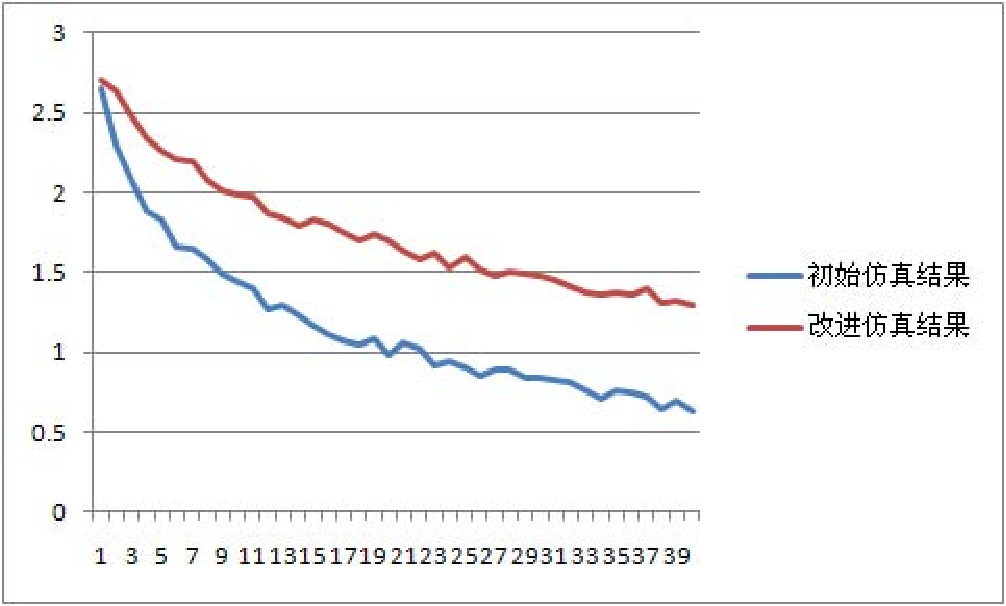
\includegraphics{improve7.pdf}}
  % GNUPLOT: LaTeX picture
\setlength{\unitlength}{0.240900pt}
\ifx\plotpoint\undefined\newsavebox{\plotpoint}\fi
\sbox{\plotpoint}{\rule[-0.200pt]{0.400pt}{0.400pt}}%
\begin{picture}(1500,900)(0,0)
\sbox{\plotpoint}{\rule[-0.200pt]{0.400pt}{0.400pt}}%
\put(131.0,82.0){\rule[-0.200pt]{4.818pt}{0.400pt}}
\put(111,82){\makebox(0,0)[r]{-1}}
\put(1419.0,82.0){\rule[-0.200pt]{4.818pt}{0.400pt}}
\put(131.0,237.0){\rule[-0.200pt]{4.818pt}{0.400pt}}
\put(111,237){\makebox(0,0)[r]{ 0}}
\put(1419.0,237.0){\rule[-0.200pt]{4.818pt}{0.400pt}}
\put(131.0,393.0){\rule[-0.200pt]{4.818pt}{0.400pt}}
\put(111,393){\makebox(0,0)[r]{ 1}}
\put(1419.0,393.0){\rule[-0.200pt]{4.818pt}{0.400pt}}
\put(131.0,548.0){\rule[-0.200pt]{4.818pt}{0.400pt}}
\put(111,548){\makebox(0,0)[r]{ 2}}
\put(1419.0,548.0){\rule[-0.200pt]{4.818pt}{0.400pt}}
\put(131.0,704.0){\rule[-0.200pt]{4.818pt}{0.400pt}}
\put(111,704){\makebox(0,0)[r]{ 3}}
\put(1419.0,704.0){\rule[-0.200pt]{4.818pt}{0.400pt}}
\put(131.0,82.0){\rule[-0.200pt]{0.400pt}{4.818pt}}
\put(131,41){\makebox(0,0){ 1}}
\put(131.0,839.0){\rule[-0.200pt]{0.400pt}{4.818pt}}
\put(198.0,82.0){\rule[-0.200pt]{0.400pt}{4.818pt}}
\put(198,41){\makebox(0,0){ 3}}
\put(198.0,839.0){\rule[-0.200pt]{0.400pt}{4.818pt}}
\put(265.0,82.0){\rule[-0.200pt]{0.400pt}{4.818pt}}
\put(265,41){\makebox(0,0){ 5}}
\put(265.0,839.0){\rule[-0.200pt]{0.400pt}{4.818pt}}
\put(332.0,82.0){\rule[-0.200pt]{0.400pt}{4.818pt}}
\put(332,41){\makebox(0,0){ 7}}
\put(332.0,839.0){\rule[-0.200pt]{0.400pt}{4.818pt}}
\put(399.0,82.0){\rule[-0.200pt]{0.400pt}{4.818pt}}
\put(399,41){\makebox(0,0){ 9}}
\put(399.0,839.0){\rule[-0.200pt]{0.400pt}{4.818pt}}
\put(466.0,82.0){\rule[-0.200pt]{0.400pt}{4.818pt}}
\put(466,41){\makebox(0,0){ 11}}
\put(466.0,839.0){\rule[-0.200pt]{0.400pt}{4.818pt}}
\put(533.0,82.0){\rule[-0.200pt]{0.400pt}{4.818pt}}
\put(533,41){\makebox(0,0){ 13}}
\put(533.0,839.0){\rule[-0.200pt]{0.400pt}{4.818pt}}
\put(601.0,82.0){\rule[-0.200pt]{0.400pt}{4.818pt}}
\put(601,41){\makebox(0,0){ 15}}
\put(601.0,839.0){\rule[-0.200pt]{0.400pt}{4.818pt}}
\put(668.0,82.0){\rule[-0.200pt]{0.400pt}{4.818pt}}
\put(668,41){\makebox(0,0){ 17}}
\put(668.0,839.0){\rule[-0.200pt]{0.400pt}{4.818pt}}
\put(735.0,82.0){\rule[-0.200pt]{0.400pt}{4.818pt}}
\put(735,41){\makebox(0,0){ 19}}
\put(735.0,839.0){\rule[-0.200pt]{0.400pt}{4.818pt}}
\put(802.0,82.0){\rule[-0.200pt]{0.400pt}{4.818pt}}
\put(802,41){\makebox(0,0){ 21}}
\put(802.0,839.0){\rule[-0.200pt]{0.400pt}{4.818pt}}
\put(869.0,82.0){\rule[-0.200pt]{0.400pt}{4.818pt}}
\put(869,41){\makebox(0,0){ 23}}
\put(869.0,839.0){\rule[-0.200pt]{0.400pt}{4.818pt}}
\put(936.0,82.0){\rule[-0.200pt]{0.400pt}{4.818pt}}
\put(936,41){\makebox(0,0){ 25}}
\put(936.0,839.0){\rule[-0.200pt]{0.400pt}{4.818pt}}
\put(1003.0,82.0){\rule[-0.200pt]{0.400pt}{4.818pt}}
\put(1003,41){\makebox(0,0){ 27}}
\put(1003.0,839.0){\rule[-0.200pt]{0.400pt}{4.818pt}}
\put(1070.0,82.0){\rule[-0.200pt]{0.400pt}{4.818pt}}
\put(1070,41){\makebox(0,0){ 29}}
\put(1070.0,839.0){\rule[-0.200pt]{0.400pt}{4.818pt}}
\put(1137.0,82.0){\rule[-0.200pt]{0.400pt}{4.818pt}}
\put(1137,41){\makebox(0,0){ 31}}
\put(1137.0,839.0){\rule[-0.200pt]{0.400pt}{4.818pt}}
\put(1204.0,82.0){\rule[-0.200pt]{0.400pt}{4.818pt}}
\put(1204,41){\makebox(0,0){ 33}}
\put(1204.0,839.0){\rule[-0.200pt]{0.400pt}{4.818pt}}
\put(1271.0,82.0){\rule[-0.200pt]{0.400pt}{4.818pt}}
\put(1271,41){\makebox(0,0){ 35}}
\put(1271.0,839.0){\rule[-0.200pt]{0.400pt}{4.818pt}}
\put(1338.0,82.0){\rule[-0.200pt]{0.400pt}{4.818pt}}
\put(1338,41){\makebox(0,0){ 37}}
\put(1338.0,839.0){\rule[-0.200pt]{0.400pt}{4.818pt}}
\put(1405.0,82.0){\rule[-0.200pt]{0.400pt}{4.818pt}}
\put(1405,41){\makebox(0,0){ 39}}
\put(1405.0,839.0){\rule[-0.200pt]{0.400pt}{4.818pt}}
\put(131.0,82.0){\rule[-0.200pt]{0.400pt}{187.179pt}}
\put(131.0,82.0){\rule[-0.200pt]{315.097pt}{0.400pt}}
\put(1439.0,82.0){\rule[-0.200pt]{0.400pt}{187.179pt}}
\put(131.0,859.0){\rule[-0.200pt]{315.097pt}{0.400pt}}
\put(30,470){\makebox(0,0){\rotatebox{90}{用户贡献}}}
\put(785,-10){\makebox(0,0){月度}}
\put(1279,819){\makebox(0,0)[r]{仿真数据}}
\put(1299.0,819.0){\rule[-0.200pt]{24.090pt}{0.400pt}}
\put(131,646){\usebox{\plotpoint}}
\multiput(131.58,643.05)(0.498,-0.766){65}{\rule{0.120pt}{0.712pt}}
\multiput(130.17,644.52)(34.000,-50.523){2}{\rule{0.400pt}{0.356pt}}
\multiput(165.00,592.92)(0.549,-0.497){57}{\rule{0.540pt}{0.120pt}}
\multiput(165.00,593.17)(31.879,-30.000){2}{\rule{0.270pt}{0.400pt}}
\multiput(198.00,562.92)(0.607,-0.497){53}{\rule{0.586pt}{0.120pt}}
\multiput(198.00,563.17)(32.784,-28.000){2}{\rule{0.293pt}{0.400pt}}
\multiput(232.00,534.92)(0.979,-0.495){31}{\rule{0.876pt}{0.119pt}}
\multiput(232.00,535.17)(31.181,-17.000){2}{\rule{0.438pt}{0.400pt}}
\multiput(265.00,517.92)(1.231,-0.494){25}{\rule{1.071pt}{0.119pt}}
\multiput(265.00,518.17)(31.776,-14.000){2}{\rule{0.536pt}{0.400pt}}
\multiput(299.00,503.92)(0.874,-0.495){35}{\rule{0.795pt}{0.119pt}}
\multiput(299.00,504.17)(31.350,-19.000){2}{\rule{0.397pt}{0.400pt}}
\multiput(332.00,484.93)(2.211,-0.488){13}{\rule{1.800pt}{0.117pt}}
\multiput(332.00,485.17)(30.264,-8.000){2}{\rule{0.900pt}{0.400pt}}
\multiput(366.00,476.93)(3.604,-0.477){7}{\rule{2.740pt}{0.115pt}}
\multiput(366.00,477.17)(27.313,-5.000){2}{\rule{1.370pt}{0.400pt}}
\multiput(399.00,471.92)(1.329,-0.493){23}{\rule{1.146pt}{0.119pt}}
\multiput(399.00,472.17)(31.621,-13.000){2}{\rule{0.573pt}{0.400pt}}
\multiput(433.00,458.92)(1.041,-0.494){29}{\rule{0.925pt}{0.119pt}}
\multiput(433.00,459.17)(31.080,-16.000){2}{\rule{0.463pt}{0.400pt}}
\put(466,443.67){\rule{8.191pt}{0.400pt}}
\multiput(466.00,443.17)(17.000,1.000){2}{\rule{4.095pt}{0.400pt}}
\multiput(500.00,443.93)(3.604,-0.477){7}{\rule{2.740pt}{0.115pt}}
\multiput(500.00,444.17)(27.313,-5.000){2}{\rule{1.370pt}{0.400pt}}
\multiput(533.00,438.93)(2.552,-0.485){11}{\rule{2.043pt}{0.117pt}}
\multiput(533.00,439.17)(29.760,-7.000){2}{\rule{1.021pt}{0.400pt}}
\multiput(567.00,431.93)(3.716,-0.477){7}{\rule{2.820pt}{0.115pt}}
\multiput(567.00,432.17)(28.147,-5.000){2}{\rule{1.410pt}{0.400pt}}
\multiput(601.00,426.93)(3.604,-0.477){7}{\rule{2.740pt}{0.115pt}}
\multiput(601.00,427.17)(27.313,-5.000){2}{\rule{1.370pt}{0.400pt}}
\multiput(634.00,421.93)(3.716,-0.477){7}{\rule{2.820pt}{0.115pt}}
\multiput(634.00,422.17)(28.147,-5.000){2}{\rule{1.410pt}{0.400pt}}
\multiput(668.00,416.93)(1.893,-0.489){15}{\rule{1.567pt}{0.118pt}}
\multiput(668.00,417.17)(29.748,-9.000){2}{\rule{0.783pt}{0.400pt}}
\multiput(701.00,407.94)(4.868,-0.468){5}{\rule{3.500pt}{0.113pt}}
\multiput(701.00,408.17)(26.736,-4.000){2}{\rule{1.750pt}{0.400pt}}
\multiput(735.00,403.93)(2.932,-0.482){9}{\rule{2.300pt}{0.116pt}}
\multiput(735.00,404.17)(28.226,-6.000){2}{\rule{1.150pt}{0.400pt}}
\multiput(768.00,397.93)(2.552,-0.485){11}{\rule{2.043pt}{0.117pt}}
\multiput(768.00,398.17)(29.760,-7.000){2}{\rule{1.021pt}{0.400pt}}
\put(802,391.67){\rule{7.950pt}{0.400pt}}
\multiput(802.00,391.17)(16.500,1.000){2}{\rule{3.975pt}{0.400pt}}
\multiput(835.00,391.93)(2.211,-0.488){13}{\rule{1.800pt}{0.117pt}}
\multiput(835.00,392.17)(30.264,-8.000){2}{\rule{0.900pt}{0.400pt}}
\multiput(869.00,383.93)(2.932,-0.482){9}{\rule{2.300pt}{0.116pt}}
\multiput(869.00,384.17)(28.226,-6.000){2}{\rule{1.150pt}{0.400pt}}
\multiput(902.00,377.95)(7.383,-0.447){3}{\rule{4.633pt}{0.108pt}}
\multiput(902.00,378.17)(24.383,-3.000){2}{\rule{2.317pt}{0.400pt}}
\put(936,376.17){\rule{6.700pt}{0.400pt}}
\multiput(936.00,375.17)(19.094,2.000){2}{\rule{3.350pt}{0.400pt}}
\multiput(969.00,376.94)(4.868,-0.468){5}{\rule{3.500pt}{0.113pt}}
\multiput(969.00,377.17)(26.736,-4.000){2}{\rule{1.750pt}{0.400pt}}
\multiput(1003.00,372.93)(2.211,-0.488){13}{\rule{1.800pt}{0.117pt}}
\multiput(1003.00,373.17)(30.264,-8.000){2}{\rule{0.900pt}{0.400pt}}
\multiput(1037.00,364.93)(2.476,-0.485){11}{\rule{1.986pt}{0.117pt}}
\multiput(1037.00,365.17)(28.879,-7.000){2}{\rule{0.993pt}{0.400pt}}
\put(1070,357.67){\rule{8.191pt}{0.400pt}}
\multiput(1070.00,358.17)(17.000,-1.000){2}{\rule{4.095pt}{0.400pt}}
\multiput(1104.00,356.94)(4.722,-0.468){5}{\rule{3.400pt}{0.113pt}}
\multiput(1104.00,357.17)(25.943,-4.000){2}{\rule{1.700pt}{0.400pt}}
\multiput(1137.00,352.94)(4.868,-0.468){5}{\rule{3.500pt}{0.113pt}}
\multiput(1137.00,353.17)(26.736,-4.000){2}{\rule{1.750pt}{0.400pt}}
\put(1171,348.67){\rule{7.950pt}{0.400pt}}
\multiput(1171.00,349.17)(16.500,-1.000){2}{\rule{3.975pt}{0.400pt}}
\put(1238,347.17){\rule{6.700pt}{0.400pt}}
\multiput(1238.00,348.17)(19.094,-2.000){2}{\rule{3.350pt}{0.400pt}}
\put(1271,345.67){\rule{8.191pt}{0.400pt}}
\multiput(1271.00,346.17)(17.000,-1.000){2}{\rule{4.095pt}{0.400pt}}
\put(1305,345.67){\rule{7.950pt}{0.400pt}}
\multiput(1305.00,345.17)(16.500,1.000){2}{\rule{3.975pt}{0.400pt}}
\put(1204.0,349.0){\rule[-0.200pt]{8.191pt}{0.400pt}}
\multiput(1372.00,345.93)(2.476,-0.485){11}{\rule{1.986pt}{0.117pt}}
\multiput(1372.00,346.17)(28.879,-7.000){2}{\rule{0.993pt}{0.400pt}}
\put(1405,338.17){\rule{6.900pt}{0.400pt}}
\multiput(1405.00,339.17)(19.679,-2.000){2}{\rule{3.450pt}{0.400pt}}
\put(1338.0,347.0){\rule[-0.200pt]{8.191pt}{0.400pt}}
\put(1279,768){\makebox(0,0)[r]{改进数据}}
\put(1299.0,768.0){\rule[-0.200pt]{24.090pt}{0.400pt}}
\put(131,669){\usebox{\plotpoint}}
\multiput(131.00,667.92)(1.009,-0.495){31}{\rule{0.900pt}{0.119pt}}
\multiput(131.00,668.17)(32.132,-17.000){2}{\rule{0.450pt}{0.400pt}}
\multiput(165.00,650.92)(0.589,-0.497){53}{\rule{0.571pt}{0.120pt}}
\multiput(165.00,651.17)(31.814,-28.000){2}{\rule{0.286pt}{0.400pt}}
\multiput(198.00,622.92)(1.009,-0.495){31}{\rule{0.900pt}{0.119pt}}
\multiput(198.00,623.17)(32.132,-17.000){2}{\rule{0.450pt}{0.400pt}}
\multiput(232.00,605.93)(2.932,-0.482){9}{\rule{2.300pt}{0.116pt}}
\multiput(232.00,606.17)(28.226,-6.000){2}{\rule{1.150pt}{0.400pt}}
\multiput(265.00,599.92)(1.581,-0.492){19}{\rule{1.336pt}{0.118pt}}
\multiput(265.00,600.17)(31.226,-11.000){2}{\rule{0.668pt}{0.400pt}}
\multiput(299.00,588.92)(1.041,-0.494){29}{\rule{0.925pt}{0.119pt}}
\multiput(299.00,589.17)(31.080,-16.000){2}{\rule{0.463pt}{0.400pt}}
\multiput(332.00,572.92)(1.444,-0.492){21}{\rule{1.233pt}{0.119pt}}
\multiput(332.00,573.17)(31.440,-12.000){2}{\rule{0.617pt}{0.400pt}}
\multiput(366.00,560.92)(1.113,-0.494){27}{\rule{0.980pt}{0.119pt}}
\multiput(366.00,561.17)(30.966,-15.000){2}{\rule{0.490pt}{0.400pt}}
\multiput(399.00,545.93)(2.211,-0.488){13}{\rule{1.800pt}{0.117pt}}
\multiput(399.00,546.17)(30.264,-8.000){2}{\rule{0.900pt}{0.400pt}}
\put(433,537.17){\rule{6.700pt}{0.400pt}}
\multiput(433.00,538.17)(19.094,-2.000){2}{\rule{3.350pt}{0.400pt}}
\multiput(466.00,535.93)(1.951,-0.489){15}{\rule{1.611pt}{0.118pt}}
\multiput(466.00,536.17)(30.656,-9.000){2}{\rule{0.806pt}{0.400pt}}
\multiput(500.00,526.93)(2.145,-0.488){13}{\rule{1.750pt}{0.117pt}}
\multiput(500.00,527.17)(29.368,-8.000){2}{\rule{0.875pt}{0.400pt}}
\multiput(533.00,518.92)(1.581,-0.492){19}{\rule{1.336pt}{0.118pt}}
\multiput(533.00,519.17)(31.226,-11.000){2}{\rule{0.668pt}{0.400pt}}
\multiput(567.00,507.92)(1.147,-0.494){27}{\rule{1.007pt}{0.119pt}}
\multiput(567.00,508.17)(31.911,-15.000){2}{\rule{0.503pt}{0.400pt}}
\multiput(601.00,492.93)(2.932,-0.482){9}{\rule{2.300pt}{0.116pt}}
\multiput(601.00,493.17)(28.226,-6.000){2}{\rule{1.150pt}{0.400pt}}
\multiput(634.00,486.94)(4.868,-0.468){5}{\rule{3.500pt}{0.113pt}}
\multiput(634.00,487.17)(26.736,-4.000){2}{\rule{1.750pt}{0.400pt}}
\multiput(668.00,482.93)(2.476,-0.485){11}{\rule{1.986pt}{0.117pt}}
\multiput(668.00,483.17)(28.879,-7.000){2}{\rule{0.993pt}{0.400pt}}
\multiput(701.00,475.95)(7.383,-0.447){3}{\rule{4.633pt}{0.108pt}}
\multiput(701.00,476.17)(24.383,-3.000){2}{\rule{2.317pt}{0.400pt}}
\multiput(735.00,472.95)(7.160,-0.447){3}{\rule{4.500pt}{0.108pt}}
\multiput(735.00,473.17)(23.660,-3.000){2}{\rule{2.250pt}{0.400pt}}
\multiput(768.00,469.93)(3.716,-0.477){7}{\rule{2.820pt}{0.115pt}}
\multiput(768.00,470.17)(28.147,-5.000){2}{\rule{1.410pt}{0.400pt}}
\multiput(802.00,464.93)(2.145,-0.488){13}{\rule{1.750pt}{0.117pt}}
\multiput(802.00,465.17)(29.368,-8.000){2}{\rule{0.875pt}{0.400pt}}
\multiput(835.00,456.93)(3.716,-0.477){7}{\rule{2.820pt}{0.115pt}}
\multiput(835.00,457.17)(28.147,-5.000){2}{\rule{1.410pt}{0.400pt}}
\multiput(869.00,451.93)(1.893,-0.489){15}{\rule{1.567pt}{0.118pt}}
\multiput(869.00,452.17)(29.748,-9.000){2}{\rule{0.783pt}{0.400pt}}
\multiput(902.00,442.93)(3.022,-0.482){9}{\rule{2.367pt}{0.116pt}}
\multiput(902.00,443.17)(29.088,-6.000){2}{\rule{1.183pt}{0.400pt}}
\multiput(936.00,436.93)(2.145,-0.488){13}{\rule{1.750pt}{0.117pt}}
\multiput(936.00,437.17)(29.368,-8.000){2}{\rule{0.875pt}{0.400pt}}
\multiput(969.00,428.93)(2.211,-0.488){13}{\rule{1.800pt}{0.117pt}}
\multiput(969.00,429.17)(30.264,-8.000){2}{\rule{0.900pt}{0.400pt}}
\multiput(1003.00,420.94)(4.868,-0.468){5}{\rule{3.500pt}{0.113pt}}
\multiput(1003.00,421.17)(26.736,-4.000){2}{\rule{1.750pt}{0.400pt}}
\multiput(1037.00,416.93)(3.604,-0.477){7}{\rule{2.740pt}{0.115pt}}
\multiput(1037.00,417.17)(27.313,-5.000){2}{\rule{1.370pt}{0.400pt}}
\multiput(1070.00,411.93)(2.211,-0.488){13}{\rule{1.800pt}{0.117pt}}
\multiput(1070.00,412.17)(30.264,-8.000){2}{\rule{0.900pt}{0.400pt}}
\multiput(1104.00,403.92)(1.401,-0.492){21}{\rule{1.200pt}{0.119pt}}
\multiput(1104.00,404.17)(30.509,-12.000){2}{\rule{0.600pt}{0.400pt}}
\put(1137,391.17){\rule{6.900pt}{0.400pt}}
\multiput(1137.00,392.17)(19.679,-2.000){2}{\rule{3.450pt}{0.400pt}}
\put(1171,389.67){\rule{7.950pt}{0.400pt}}
\multiput(1171.00,390.17)(16.500,-1.000){2}{\rule{3.975pt}{0.400pt}}
\multiput(1204.00,388.93)(3.716,-0.477){7}{\rule{2.820pt}{0.115pt}}
\multiput(1204.00,389.17)(28.147,-5.000){2}{\rule{1.410pt}{0.400pt}}
\multiput(1238.00,383.95)(7.160,-0.447){3}{\rule{4.500pt}{0.108pt}}
\multiput(1238.00,384.17)(23.660,-3.000){2}{\rule{2.250pt}{0.400pt}}
\multiput(1271.00,380.93)(3.716,-0.477){7}{\rule{2.820pt}{0.115pt}}
\multiput(1271.00,381.17)(28.147,-5.000){2}{\rule{1.410pt}{0.400pt}}
\multiput(1305.00,375.93)(3.604,-0.477){7}{\rule{2.740pt}{0.115pt}}
\multiput(1305.00,376.17)(27.313,-5.000){2}{\rule{1.370pt}{0.400pt}}
\put(1338,370.67){\rule{8.191pt}{0.400pt}}
\multiput(1338.00,371.17)(17.000,-1.000){2}{\rule{4.095pt}{0.400pt}}
\put(1372,369.17){\rule{6.700pt}{0.400pt}}
\multiput(1372.00,370.17)(19.094,-2.000){2}{\rule{3.350pt}{0.400pt}}
\put(131,669){\makebox(0,0){$+$}}
\put(165,652){\makebox(0,0){$+$}}
\put(198,624){\makebox(0,0){$+$}}
\put(232,607){\makebox(0,0){$+$}}
\put(265,601){\makebox(0,0){$+$}}
\put(299,590){\makebox(0,0){$+$}}
\put(332,574){\makebox(0,0){$+$}}
\put(366,562){\makebox(0,0){$+$}}
\put(399,547){\makebox(0,0){$+$}}
\put(433,539){\makebox(0,0){$+$}}
\put(466,537){\makebox(0,0){$+$}}
\put(500,528){\makebox(0,0){$+$}}
\put(533,520){\makebox(0,0){$+$}}
\put(567,509){\makebox(0,0){$+$}}
\put(601,494){\makebox(0,0){$+$}}
\put(634,488){\makebox(0,0){$+$}}
\put(668,484){\makebox(0,0){$+$}}
\put(701,477){\makebox(0,0){$+$}}
\put(735,474){\makebox(0,0){$+$}}
\put(768,471){\makebox(0,0){$+$}}
\put(802,466){\makebox(0,0){$+$}}
\put(835,458){\makebox(0,0){$+$}}
\put(869,453){\makebox(0,0){$+$}}
\put(902,444){\makebox(0,0){$+$}}
\put(936,438){\makebox(0,0){$+$}}
\put(969,430){\makebox(0,0){$+$}}
\put(1003,422){\makebox(0,0){$+$}}
\put(1037,418){\makebox(0,0){$+$}}
\put(1070,413){\makebox(0,0){$+$}}
\put(1104,405){\makebox(0,0){$+$}}
\put(1137,393){\makebox(0,0){$+$}}
\put(1171,391){\makebox(0,0){$+$}}
\put(1204,390){\makebox(0,0){$+$}}
\put(1238,385){\makebox(0,0){$+$}}
\put(1271,382){\makebox(0,0){$+$}}
\put(1305,377){\makebox(0,0){$+$}}
\put(1338,372){\makebox(0,0){$+$}}
\put(1372,371){\makebox(0,0){$+$}}
\put(1405,369){\makebox(0,0){$+$}}
\put(1439,369){\makebox(0,0){$+$}}
\put(1349,768){\makebox(0,0){$+$}}
\put(1405.0,369.0){\rule[-0.200pt]{8.191pt}{0.400pt}}
\put(131.0,82.0){\rule[-0.200pt]{0.400pt}{187.179pt}}
\put(131.0,82.0){\rule[-0.200pt]{315.097pt}{0.400pt}}
\put(1439.0,82.0){\rule[-0.200pt]{0.400pt}{187.179pt}}
\put(131.0,859.0){\rule[-0.200pt]{315.097pt}{0.400pt}}
\end{picture}

  \caption{\small{\textbf{提升内容维护者个体动机的仿真结果}}}
  \label{fig:improve7}
\end{figure}

\begin{figure}[!htb]
  \centering
  %\scalebox{0.65}{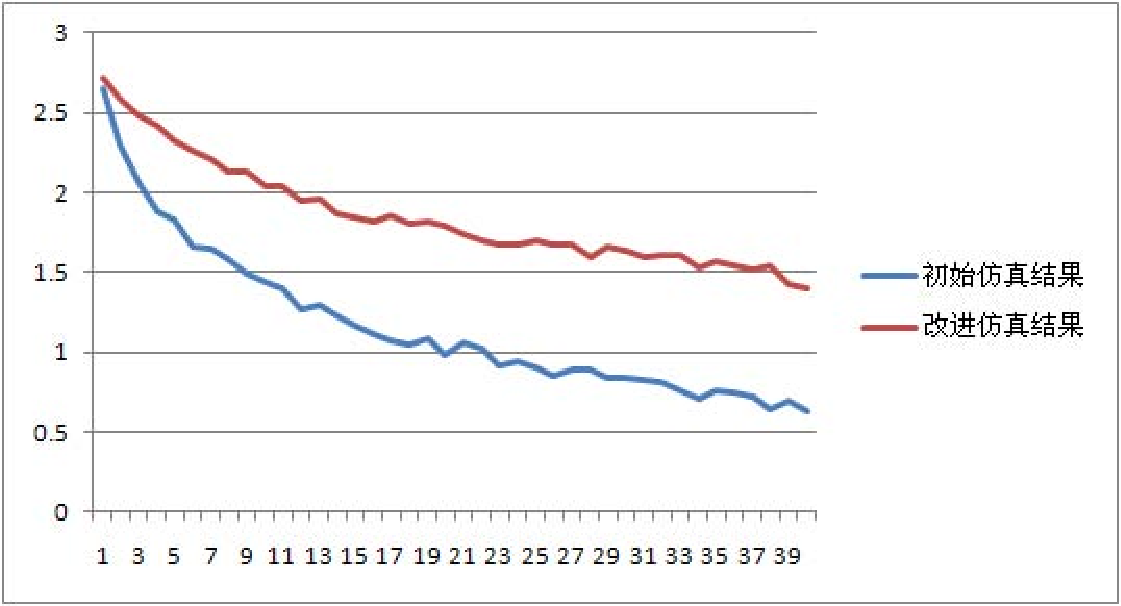
\includegraphics{improve8.pdf}}
  % GNUPLOT: LaTeX picture
\setlength{\unitlength}{0.240900pt}
\ifx\plotpoint\undefined\newsavebox{\plotpoint}\fi
\begin{picture}(1500,900)(0,0)
\sbox{\plotpoint}{\rule[-0.200pt]{0.400pt}{0.400pt}}%
\put(131.0,82.0){\rule[-0.200pt]{4.818pt}{0.400pt}}
\put(111,82){\makebox(0,0)[r]{-1}}
\put(1419.0,82.0){\rule[-0.200pt]{4.818pt}{0.400pt}}
\put(131.0,237.0){\rule[-0.200pt]{4.818pt}{0.400pt}}
\put(111,237){\makebox(0,0)[r]{ 0}}
\put(1419.0,237.0){\rule[-0.200pt]{4.818pt}{0.400pt}}
\put(131.0,393.0){\rule[-0.200pt]{4.818pt}{0.400pt}}
\put(111,393){\makebox(0,0)[r]{ 1}}
\put(1419.0,393.0){\rule[-0.200pt]{4.818pt}{0.400pt}}
\put(131.0,548.0){\rule[-0.200pt]{4.818pt}{0.400pt}}
\put(111,548){\makebox(0,0)[r]{ 2}}
\put(1419.0,548.0){\rule[-0.200pt]{4.818pt}{0.400pt}}
\put(131.0,704.0){\rule[-0.200pt]{4.818pt}{0.400pt}}
\put(111,704){\makebox(0,0)[r]{ 3}}
\put(1419.0,704.0){\rule[-0.200pt]{4.818pt}{0.400pt}}
\put(131.0,82.0){\rule[-0.200pt]{0.400pt}{4.818pt}}
\put(131,41){\makebox(0,0){ 1}}
\put(131.0,839.0){\rule[-0.200pt]{0.400pt}{4.818pt}}
\put(198.0,82.0){\rule[-0.200pt]{0.400pt}{4.818pt}}
\put(198,41){\makebox(0,0){ 3}}
\put(198.0,839.0){\rule[-0.200pt]{0.400pt}{4.818pt}}
\put(265.0,82.0){\rule[-0.200pt]{0.400pt}{4.818pt}}
\put(265,41){\makebox(0,0){ 5}}
\put(265.0,839.0){\rule[-0.200pt]{0.400pt}{4.818pt}}
\put(332.0,82.0){\rule[-0.200pt]{0.400pt}{4.818pt}}
\put(332,41){\makebox(0,0){ 7}}
\put(332.0,839.0){\rule[-0.200pt]{0.400pt}{4.818pt}}
\put(399.0,82.0){\rule[-0.200pt]{0.400pt}{4.818pt}}
\put(399,41){\makebox(0,0){ 9}}
\put(399.0,839.0){\rule[-0.200pt]{0.400pt}{4.818pt}}
\put(466.0,82.0){\rule[-0.200pt]{0.400pt}{4.818pt}}
\put(466,41){\makebox(0,0){ 11}}
\put(466.0,839.0){\rule[-0.200pt]{0.400pt}{4.818pt}}
\put(533.0,82.0){\rule[-0.200pt]{0.400pt}{4.818pt}}
\put(533,41){\makebox(0,0){ 13}}
\put(533.0,839.0){\rule[-0.200pt]{0.400pt}{4.818pt}}
\put(601.0,82.0){\rule[-0.200pt]{0.400pt}{4.818pt}}
\put(601,41){\makebox(0,0){ 15}}
\put(601.0,839.0){\rule[-0.200pt]{0.400pt}{4.818pt}}
\put(668.0,82.0){\rule[-0.200pt]{0.400pt}{4.818pt}}
\put(668,41){\makebox(0,0){ 17}}
\put(668.0,839.0){\rule[-0.200pt]{0.400pt}{4.818pt}}
\put(735.0,82.0){\rule[-0.200pt]{0.400pt}{4.818pt}}
\put(735,41){\makebox(0,0){ 19}}
\put(735.0,839.0){\rule[-0.200pt]{0.400pt}{4.818pt}}
\put(802.0,82.0){\rule[-0.200pt]{0.400pt}{4.818pt}}
\put(802,41){\makebox(0,0){ 21}}
\put(802.0,839.0){\rule[-0.200pt]{0.400pt}{4.818pt}}
\put(869.0,82.0){\rule[-0.200pt]{0.400pt}{4.818pt}}
\put(869,41){\makebox(0,0){ 23}}
\put(869.0,839.0){\rule[-0.200pt]{0.400pt}{4.818pt}}
\put(936.0,82.0){\rule[-0.200pt]{0.400pt}{4.818pt}}
\put(936,41){\makebox(0,0){ 25}}
\put(936.0,839.0){\rule[-0.200pt]{0.400pt}{4.818pt}}
\put(1003.0,82.0){\rule[-0.200pt]{0.400pt}{4.818pt}}
\put(1003,41){\makebox(0,0){ 27}}
\put(1003.0,839.0){\rule[-0.200pt]{0.400pt}{4.818pt}}
\put(1070.0,82.0){\rule[-0.200pt]{0.400pt}{4.818pt}}
\put(1070,41){\makebox(0,0){ 29}}
\put(1070.0,839.0){\rule[-0.200pt]{0.400pt}{4.818pt}}
\put(1137.0,82.0){\rule[-0.200pt]{0.400pt}{4.818pt}}
\put(1137,41){\makebox(0,0){ 31}}
\put(1137.0,839.0){\rule[-0.200pt]{0.400pt}{4.818pt}}
\put(1204.0,82.0){\rule[-0.200pt]{0.400pt}{4.818pt}}
\put(1204,41){\makebox(0,0){ 33}}
\put(1204.0,839.0){\rule[-0.200pt]{0.400pt}{4.818pt}}
\put(1271.0,82.0){\rule[-0.200pt]{0.400pt}{4.818pt}}
\put(1271,41){\makebox(0,0){ 35}}
\put(1271.0,839.0){\rule[-0.200pt]{0.400pt}{4.818pt}}
\put(1338.0,82.0){\rule[-0.200pt]{0.400pt}{4.818pt}}
\put(1338,41){\makebox(0,0){ 37}}
\put(1338.0,839.0){\rule[-0.200pt]{0.400pt}{4.818pt}}
\put(1405.0,82.0){\rule[-0.200pt]{0.400pt}{4.818pt}}
\put(1405,41){\makebox(0,0){ 39}}
\put(1405.0,839.0){\rule[-0.200pt]{0.400pt}{4.818pt}}
\put(131.0,82.0){\rule[-0.200pt]{0.400pt}{187.179pt}}
\put(131.0,82.0){\rule[-0.200pt]{315.097pt}{0.400pt}}
\put(1439.0,82.0){\rule[-0.200pt]{0.400pt}{187.179pt}}
\put(131.0,859.0){\rule[-0.200pt]{315.097pt}{0.400pt}}
\put(30,470){\makebox(0,0){\rotatebox{90}{用户贡献}}}
\put(785,-10){\makebox(0,0){月度}}
\put(1279,819){\makebox(0,0)[r]{仿真数据}}
\put(1299.0,819.0){\rule[-0.200pt]{24.090pt}{0.400pt}}
\put(131,646){\usebox{\plotpoint}}
\multiput(131.58,643.05)(0.498,-0.766){65}{\rule{0.120pt}{0.712pt}}
\multiput(130.17,644.52)(34.000,-50.523){2}{\rule{0.400pt}{0.356pt}}
\multiput(165.00,592.92)(0.549,-0.497){57}{\rule{0.540pt}{0.120pt}}
\multiput(165.00,593.17)(31.879,-30.000){2}{\rule{0.270pt}{0.400pt}}
\multiput(198.00,562.92)(0.607,-0.497){53}{\rule{0.586pt}{0.120pt}}
\multiput(198.00,563.17)(32.784,-28.000){2}{\rule{0.293pt}{0.400pt}}
\multiput(232.00,534.92)(0.979,-0.495){31}{\rule{0.876pt}{0.119pt}}
\multiput(232.00,535.17)(31.181,-17.000){2}{\rule{0.438pt}{0.400pt}}
\multiput(265.00,517.92)(1.231,-0.494){25}{\rule{1.071pt}{0.119pt}}
\multiput(265.00,518.17)(31.776,-14.000){2}{\rule{0.536pt}{0.400pt}}
\multiput(299.00,503.92)(0.874,-0.495){35}{\rule{0.795pt}{0.119pt}}
\multiput(299.00,504.17)(31.350,-19.000){2}{\rule{0.397pt}{0.400pt}}
\multiput(332.00,484.93)(2.211,-0.488){13}{\rule{1.800pt}{0.117pt}}
\multiput(332.00,485.17)(30.264,-8.000){2}{\rule{0.900pt}{0.400pt}}
\multiput(366.00,476.93)(3.604,-0.477){7}{\rule{2.740pt}{0.115pt}}
\multiput(366.00,477.17)(27.313,-5.000){2}{\rule{1.370pt}{0.400pt}}
\multiput(399.00,471.92)(1.329,-0.493){23}{\rule{1.146pt}{0.119pt}}
\multiput(399.00,472.17)(31.621,-13.000){2}{\rule{0.573pt}{0.400pt}}
\multiput(433.00,458.92)(1.041,-0.494){29}{\rule{0.925pt}{0.119pt}}
\multiput(433.00,459.17)(31.080,-16.000){2}{\rule{0.463pt}{0.400pt}}
\put(466,443.67){\rule{8.191pt}{0.400pt}}
\multiput(466.00,443.17)(17.000,1.000){2}{\rule{4.095pt}{0.400pt}}
\multiput(500.00,443.93)(3.604,-0.477){7}{\rule{2.740pt}{0.115pt}}
\multiput(500.00,444.17)(27.313,-5.000){2}{\rule{1.370pt}{0.400pt}}
\multiput(533.00,438.93)(2.552,-0.485){11}{\rule{2.043pt}{0.117pt}}
\multiput(533.00,439.17)(29.760,-7.000){2}{\rule{1.021pt}{0.400pt}}
\multiput(567.00,431.93)(3.716,-0.477){7}{\rule{2.820pt}{0.115pt}}
\multiput(567.00,432.17)(28.147,-5.000){2}{\rule{1.410pt}{0.400pt}}
\multiput(601.00,426.93)(3.604,-0.477){7}{\rule{2.740pt}{0.115pt}}
\multiput(601.00,427.17)(27.313,-5.000){2}{\rule{1.370pt}{0.400pt}}
\multiput(634.00,421.93)(3.716,-0.477){7}{\rule{2.820pt}{0.115pt}}
\multiput(634.00,422.17)(28.147,-5.000){2}{\rule{1.410pt}{0.400pt}}
\multiput(668.00,416.93)(1.893,-0.489){15}{\rule{1.567pt}{0.118pt}}
\multiput(668.00,417.17)(29.748,-9.000){2}{\rule{0.783pt}{0.400pt}}
\multiput(701.00,407.94)(4.868,-0.468){5}{\rule{3.500pt}{0.113pt}}
\multiput(701.00,408.17)(26.736,-4.000){2}{\rule{1.750pt}{0.400pt}}
\multiput(735.00,403.93)(2.932,-0.482){9}{\rule{2.300pt}{0.116pt}}
\multiput(735.00,404.17)(28.226,-6.000){2}{\rule{1.150pt}{0.400pt}}
\multiput(768.00,397.93)(2.552,-0.485){11}{\rule{2.043pt}{0.117pt}}
\multiput(768.00,398.17)(29.760,-7.000){2}{\rule{1.021pt}{0.400pt}}
\put(802,391.67){\rule{7.950pt}{0.400pt}}
\multiput(802.00,391.17)(16.500,1.000){2}{\rule{3.975pt}{0.400pt}}
\multiput(835.00,391.93)(2.211,-0.488){13}{\rule{1.800pt}{0.117pt}}
\multiput(835.00,392.17)(30.264,-8.000){2}{\rule{0.900pt}{0.400pt}}
\multiput(869.00,383.93)(2.932,-0.482){9}{\rule{2.300pt}{0.116pt}}
\multiput(869.00,384.17)(28.226,-6.000){2}{\rule{1.150pt}{0.400pt}}
\multiput(902.00,377.95)(7.383,-0.447){3}{\rule{4.633pt}{0.108pt}}
\multiput(902.00,378.17)(24.383,-3.000){2}{\rule{2.317pt}{0.400pt}}
\put(936,376.17){\rule{6.700pt}{0.400pt}}
\multiput(936.00,375.17)(19.094,2.000){2}{\rule{3.350pt}{0.400pt}}
\multiput(969.00,376.94)(4.868,-0.468){5}{\rule{3.500pt}{0.113pt}}
\multiput(969.00,377.17)(26.736,-4.000){2}{\rule{1.750pt}{0.400pt}}
\multiput(1003.00,372.93)(2.211,-0.488){13}{\rule{1.800pt}{0.117pt}}
\multiput(1003.00,373.17)(30.264,-8.000){2}{\rule{0.900pt}{0.400pt}}
\multiput(1037.00,364.93)(2.476,-0.485){11}{\rule{1.986pt}{0.117pt}}
\multiput(1037.00,365.17)(28.879,-7.000){2}{\rule{0.993pt}{0.400pt}}
\put(1070,357.67){\rule{8.191pt}{0.400pt}}
\multiput(1070.00,358.17)(17.000,-1.000){2}{\rule{4.095pt}{0.400pt}}
\multiput(1104.00,356.94)(4.722,-0.468){5}{\rule{3.400pt}{0.113pt}}
\multiput(1104.00,357.17)(25.943,-4.000){2}{\rule{1.700pt}{0.400pt}}
\multiput(1137.00,352.94)(4.868,-0.468){5}{\rule{3.500pt}{0.113pt}}
\multiput(1137.00,353.17)(26.736,-4.000){2}{\rule{1.750pt}{0.400pt}}
\put(1171,348.67){\rule{7.950pt}{0.400pt}}
\multiput(1171.00,349.17)(16.500,-1.000){2}{\rule{3.975pt}{0.400pt}}
\put(1238,347.17){\rule{6.700pt}{0.400pt}}
\multiput(1238.00,348.17)(19.094,-2.000){2}{\rule{3.350pt}{0.400pt}}
\put(1271,345.67){\rule{8.191pt}{0.400pt}}
\multiput(1271.00,346.17)(17.000,-1.000){2}{\rule{4.095pt}{0.400pt}}
\put(1305,345.67){\rule{7.950pt}{0.400pt}}
\multiput(1305.00,345.17)(16.500,1.000){2}{\rule{3.975pt}{0.400pt}}
\put(1204.0,349.0){\rule[-0.200pt]{8.191pt}{0.400pt}}
\multiput(1372.00,345.93)(2.476,-0.485){11}{\rule{1.986pt}{0.117pt}}
\multiput(1372.00,346.17)(28.879,-7.000){2}{\rule{0.993pt}{0.400pt}}
\put(1405,338.17){\rule{6.900pt}{0.400pt}}
\multiput(1405.00,339.17)(19.679,-2.000){2}{\rule{3.450pt}{0.400pt}}
\put(1338.0,347.0){\rule[-0.200pt]{8.191pt}{0.400pt}}
\put(1279,768){\makebox(0,0)[r]{改进数据}}
\put(1299.0,768.0){\rule[-0.200pt]{24.090pt}{0.400pt}}
\put(131,671){\usebox{\plotpoint}}
\multiput(131.00,669.92)(1.073,-0.494){29}{\rule{0.950pt}{0.119pt}}
\multiput(131.00,670.17)(32.028,-16.000){2}{\rule{0.475pt}{0.400pt}}
\multiput(165.00,653.92)(0.923,-0.495){33}{\rule{0.833pt}{0.119pt}}
\multiput(165.00,654.17)(31.270,-18.000){2}{\rule{0.417pt}{0.400pt}}
\multiput(198.00,635.92)(0.855,-0.496){37}{\rule{0.780pt}{0.119pt}}
\multiput(198.00,636.17)(32.381,-20.000){2}{\rule{0.390pt}{0.400pt}}
\multiput(232.00,615.93)(2.476,-0.485){11}{\rule{1.986pt}{0.117pt}}
\multiput(232.00,616.17)(28.879,-7.000){2}{\rule{0.993pt}{0.400pt}}
\multiput(265.00,608.92)(1.581,-0.492){19}{\rule{1.336pt}{0.118pt}}
\multiput(265.00,609.17)(31.226,-11.000){2}{\rule{0.668pt}{0.400pt}}
\multiput(299.00,597.92)(1.694,-0.491){17}{\rule{1.420pt}{0.118pt}}
\multiput(299.00,598.17)(30.053,-10.000){2}{\rule{0.710pt}{0.400pt}}
\multiput(332.00,587.92)(1.231,-0.494){25}{\rule{1.071pt}{0.119pt}}
\multiput(332.00,588.17)(31.776,-14.000){2}{\rule{0.536pt}{0.400pt}}
\multiput(366.00,573.92)(1.290,-0.493){23}{\rule{1.115pt}{0.119pt}}
\multiput(366.00,574.17)(30.685,-13.000){2}{\rule{0.558pt}{0.400pt}}
\multiput(399.00,560.93)(2.211,-0.488){13}{\rule{1.800pt}{0.117pt}}
\multiput(399.00,561.17)(30.264,-8.000){2}{\rule{0.900pt}{0.400pt}}
\multiput(433.00,552.93)(1.893,-0.489){15}{\rule{1.567pt}{0.118pt}}
\multiput(433.00,553.17)(29.748,-9.000){2}{\rule{0.783pt}{0.400pt}}
\multiput(466.00,543.93)(3.022,-0.482){9}{\rule{2.367pt}{0.116pt}}
\multiput(466.00,544.17)(29.088,-6.000){2}{\rule{1.183pt}{0.400pt}}
\multiput(500.00,537.93)(3.604,-0.477){7}{\rule{2.740pt}{0.115pt}}
\multiput(500.00,538.17)(27.313,-5.000){2}{\rule{1.370pt}{0.400pt}}
\multiput(533.00,532.95)(7.383,-0.447){3}{\rule{4.633pt}{0.108pt}}
\multiput(533.00,533.17)(24.383,-3.000){2}{\rule{2.317pt}{0.400pt}}
\multiput(567.00,529.93)(3.022,-0.482){9}{\rule{2.367pt}{0.116pt}}
\multiput(567.00,530.17)(29.088,-6.000){2}{\rule{1.183pt}{0.400pt}}
\multiput(601.00,523.95)(7.160,-0.447){3}{\rule{4.500pt}{0.108pt}}
\multiput(601.00,524.17)(23.660,-3.000){2}{\rule{2.250pt}{0.400pt}}
\multiput(634.00,520.92)(1.581,-0.492){19}{\rule{1.336pt}{0.118pt}}
\multiput(634.00,521.17)(31.226,-11.000){2}{\rule{0.668pt}{0.400pt}}
\multiput(668.00,509.93)(3.604,-0.477){7}{\rule{2.740pt}{0.115pt}}
\multiput(668.00,510.17)(27.313,-5.000){2}{\rule{1.370pt}{0.400pt}}
\multiput(701.00,504.93)(3.022,-0.482){9}{\rule{2.367pt}{0.116pt}}
\multiput(701.00,505.17)(29.088,-6.000){2}{\rule{1.183pt}{0.400pt}}
\multiput(735.00,498.93)(2.932,-0.482){9}{\rule{2.300pt}{0.116pt}}
\multiput(735.00,499.17)(28.226,-6.000){2}{\rule{1.150pt}{0.400pt}}
\multiput(768.00,492.93)(3.022,-0.482){9}{\rule{2.367pt}{0.116pt}}
\multiput(768.00,493.17)(29.088,-6.000){2}{\rule{1.183pt}{0.400pt}}
\multiput(802.00,486.94)(4.722,-0.468){5}{\rule{3.400pt}{0.113pt}}
\multiput(802.00,487.17)(25.943,-4.000){2}{\rule{1.700pt}{0.400pt}}
\multiput(835.00,482.92)(1.231,-0.494){25}{\rule{1.071pt}{0.119pt}}
\multiput(835.00,483.17)(31.776,-14.000){2}{\rule{0.536pt}{0.400pt}}
\multiput(869.00,468.94)(4.722,-0.468){5}{\rule{3.400pt}{0.113pt}}
\multiput(869.00,469.17)(25.943,-4.000){2}{\rule{1.700pt}{0.400pt}}
\multiput(902.00,464.93)(3.022,-0.482){9}{\rule{2.367pt}{0.116pt}}
\multiput(902.00,465.17)(29.088,-6.000){2}{\rule{1.183pt}{0.400pt}}
\multiput(936.00,458.95)(7.160,-0.447){3}{\rule{4.500pt}{0.108pt}}
\multiput(936.00,459.17)(23.660,-3.000){2}{\rule{2.250pt}{0.400pt}}
\multiput(969.00,455.93)(2.552,-0.485){11}{\rule{2.043pt}{0.117pt}}
\multiput(969.00,456.17)(29.760,-7.000){2}{\rule{1.021pt}{0.400pt}}
\multiput(1003.00,448.94)(4.868,-0.468){5}{\rule{3.500pt}{0.113pt}}
\multiput(1003.00,449.17)(26.736,-4.000){2}{\rule{1.750pt}{0.400pt}}
\multiput(1037.00,444.93)(3.604,-0.477){7}{\rule{2.740pt}{0.115pt}}
\multiput(1037.00,445.17)(27.313,-5.000){2}{\rule{1.370pt}{0.400pt}}
\multiput(1104.00,439.93)(3.604,-0.477){7}{\rule{2.740pt}{0.115pt}}
\multiput(1104.00,440.17)(27.313,-5.000){2}{\rule{1.370pt}{0.400pt}}
\multiput(1137.00,434.93)(3.022,-0.482){9}{\rule{2.367pt}{0.116pt}}
\multiput(1137.00,435.17)(29.088,-6.000){2}{\rule{1.183pt}{0.400pt}}
\multiput(1171.00,428.93)(2.932,-0.482){9}{\rule{2.300pt}{0.116pt}}
\multiput(1171.00,429.17)(28.226,-6.000){2}{\rule{1.150pt}{0.400pt}}
\multiput(1204.00,422.93)(1.951,-0.489){15}{\rule{1.611pt}{0.118pt}}
\multiput(1204.00,423.17)(30.656,-9.000){2}{\rule{0.806pt}{0.400pt}}
\multiput(1238.00,413.93)(2.476,-0.485){11}{\rule{1.986pt}{0.117pt}}
\multiput(1238.00,414.17)(28.879,-7.000){2}{\rule{0.993pt}{0.400pt}}
\multiput(1271.00,406.95)(7.383,-0.447){3}{\rule{4.633pt}{0.108pt}}
\multiput(1271.00,407.17)(24.383,-3.000){2}{\rule{2.317pt}{0.400pt}}
\multiput(1305.00,403.95)(7.160,-0.447){3}{\rule{4.500pt}{0.108pt}}
\multiput(1305.00,404.17)(23.660,-3.000){2}{\rule{2.250pt}{0.400pt}}
\multiput(1338.00,400.93)(3.022,-0.482){9}{\rule{2.367pt}{0.116pt}}
\multiput(1338.00,401.17)(29.088,-6.000){2}{\rule{1.183pt}{0.400pt}}
\put(1372,394.17){\rule{6.700pt}{0.400pt}}
\multiput(1372.00,395.17)(19.094,-2.000){2}{\rule{3.350pt}{0.400pt}}
\put(1405,392.67){\rule{8.191pt}{0.400pt}}
\multiput(1405.00,393.17)(17.000,-1.000){2}{\rule{4.095pt}{0.400pt}}
\put(131,671){\makebox(0,0){$+$}}
\put(165,655){\makebox(0,0){$+$}}
\put(198,637){\makebox(0,0){$+$}}
\put(232,617){\makebox(0,0){$+$}}
\put(265,610){\makebox(0,0){$+$}}
\put(299,599){\makebox(0,0){$+$}}
\put(332,589){\makebox(0,0){$+$}}
\put(366,575){\makebox(0,0){$+$}}
\put(399,562){\makebox(0,0){$+$}}
\put(433,554){\makebox(0,0){$+$}}
\put(466,545){\makebox(0,0){$+$}}
\put(500,539){\makebox(0,0){$+$}}
\put(533,534){\makebox(0,0){$+$}}
\put(567,531){\makebox(0,0){$+$}}
\put(601,525){\makebox(0,0){$+$}}
\put(634,522){\makebox(0,0){$+$}}
\put(668,511){\makebox(0,0){$+$}}
\put(701,506){\makebox(0,0){$+$}}
\put(735,500){\makebox(0,0){$+$}}
\put(768,494){\makebox(0,0){$+$}}
\put(802,488){\makebox(0,0){$+$}}
\put(835,484){\makebox(0,0){$+$}}
\put(869,470){\makebox(0,0){$+$}}
\put(902,466){\makebox(0,0){$+$}}
\put(936,460){\makebox(0,0){$+$}}
\put(969,457){\makebox(0,0){$+$}}
\put(1003,450){\makebox(0,0){$+$}}
\put(1037,446){\makebox(0,0){$+$}}
\put(1070,441){\makebox(0,0){$+$}}
\put(1104,441){\makebox(0,0){$+$}}
\put(1137,436){\makebox(0,0){$+$}}
\put(1171,430){\makebox(0,0){$+$}}
\put(1204,424){\makebox(0,0){$+$}}
\put(1238,415){\makebox(0,0){$+$}}
\put(1271,408){\makebox(0,0){$+$}}
\put(1305,405){\makebox(0,0){$+$}}
\put(1338,402){\makebox(0,0){$+$}}
\put(1372,396){\makebox(0,0){$+$}}
\put(1405,394){\makebox(0,0){$+$}}
\put(1439,393){\makebox(0,0){$+$}}
\put(1349,768){\makebox(0,0){$+$}}
\put(1070.0,441.0){\rule[-0.200pt]{8.191pt}{0.400pt}}
\put(131.0,82.0){\rule[-0.200pt]{0.400pt}{187.179pt}}
\put(131.0,82.0){\rule[-0.200pt]{315.097pt}{0.400pt}}
\put(1439.0,82.0){\rule[-0.200pt]{0.400pt}{187.179pt}}
\put(131.0,859.0){\rule[-0.200pt]{315.097pt}{0.400pt}}
\end{picture}

  \caption{\small{\textbf{提升内容维护者人际间动机的仿真结果}}}
  \label{fig:improve8}
\end{figure}
满足自身的社会需求是内容维护者参与社区的主要因素。内容维护者希望借由参
与社区感受到社区的温暖和支持,渴望获得社区的接纳和认同。同时,内容维护者自身的动机
水平偏低,害怕失败,尤其对于他人的行为比较敏感,动机水平容易受到外界因
素影响。这些特点决定了社区对其支持的方向应该是从保护其协同动
机入手,努力降低其对失败的关注程度,增加个体之间的协调和互动。社区管理
者应该鼓励用户之间多沟通,
多讨论,尤其是当拒绝某个人编辑的内容时应该尽力使其了解拒绝的理由、指明
改进的方向,帮助其提升编辑的水平。这样,参与者既感受到了来自于社区的支
持,同时可以将负面的感觉降低,转而多关注自身的成功,不断提升参与的信
心,使正反馈成为主导力
量。

\subsection{边缘用户}
边缘用户同内容维护者有着类似的行为模式,但是内容贡献度更低,参与次数更
少。边缘用户的月人均贡献是所有用户中唯一低于0的群体,并且变化趋势是加
速下降。边缘用户的正贡献和负贡献的比例基本是1:1,也就是说边缘用户的所
有用户贡献正负各一半,是所有用户中比例最接近的,负反馈对其的影响也是最
大的。

根据边缘用户的动机因素模型中存在着明显的负反馈环:当各体的动机降低是,
协同行为水平也会相应降低,这会导致负反馈的减少;负反馈的减少会增强个体
的动机。但是,边缘用户的行为特点显示负反馈环并未起到主导作用,这是由于
边缘用户参与的次数非常少,以至于他们不可能通过减少参与水平来达到提升个
体动机的目的。如果提升个体的动机,那么边缘用户将能够显著提升参与程度,
并转化为内容维护者,摆脱之前越不参与动机越低,动机越低越不
参与的恶性循环。

图\ref{fig:improve9}是将边缘用户的所有动机初始水平提升$30\%$所做的仿真实验。在提升初始动
机水平后,边缘用户的参与水平得到提高,并且在更多的参与中吸取了经验,熟
悉了编辑的规则和流程,提升了编辑的质量。这时边缘用户已经转化为内容贡献
者,内容贡献度的变化趋势也由加速下降转变为减速下降。仿真结果表明初始动
机水平较低是边缘用户最大的弱点,改善这一点将有助于其从社区的外围真正融
入到社区中。

\begin{figure}[!htb]
  \centering
%  \scalebox{0.65}{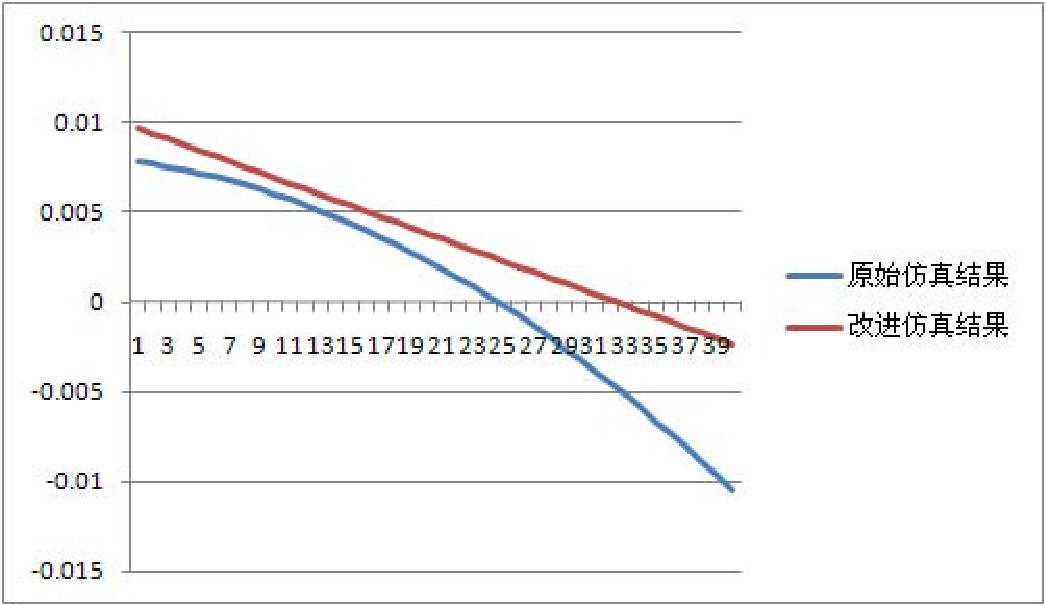
\includegraphics{improve9.pdf}}
 % GNUPLOT: LaTeX picture
\setlength{\unitlength}{0.240900pt}
\ifx\plotpoint\undefined\newsavebox{\plotpoint}\fi
\begin{picture}(1500,900)(0,0)
\sbox{\plotpoint}{\rule[-0.200pt]{0.400pt}{0.400pt}}%
\put(211.0,82.0){\rule[-0.200pt]{4.818pt}{0.400pt}}
\put(191,82){\makebox(0,0)[r]{-0.02}}
\put(1419.0,82.0){\rule[-0.200pt]{4.818pt}{0.400pt}}
\put(211.0,143.0){\rule[-0.200pt]{4.818pt}{0.400pt}}
\put(191,143){\makebox(0,0)[r]{-0.015}}
\put(1419.0,143.0){\rule[-0.200pt]{4.818pt}{0.400pt}}
\put(211.0,203.0){\rule[-0.200pt]{4.818pt}{0.400pt}}
\put(191,203){\makebox(0,0)[r]{-0.01}}
\put(1419.0,203.0){\rule[-0.200pt]{4.818pt}{0.400pt}}
\put(211.0,264.0){\rule[-0.200pt]{4.818pt}{0.400pt}}
\put(191,264){\makebox(0,0)[r]{-0.005}}
\put(1419.0,264.0){\rule[-0.200pt]{4.818pt}{0.400pt}}
\put(211.0,325.0){\rule[-0.200pt]{4.818pt}{0.400pt}}
\put(191,325){\makebox(0,0)[r]{ 0}}
\put(1419.0,325.0){\rule[-0.200pt]{4.818pt}{0.400pt}}
\put(211.0,386.0){\rule[-0.200pt]{4.818pt}{0.400pt}}
\put(191,386){\makebox(0,0)[r]{ 0.005}}
\put(1419.0,386.0){\rule[-0.200pt]{4.818pt}{0.400pt}}
\put(211.0,446.0){\rule[-0.200pt]{4.818pt}{0.400pt}}
\put(191,446){\makebox(0,0)[r]{ 0.01}}
\put(1419.0,446.0){\rule[-0.200pt]{4.818pt}{0.400pt}}
\put(211.0,507.0){\rule[-0.200pt]{4.818pt}{0.400pt}}
\put(191,507){\makebox(0,0)[r]{ 0.015}}
\put(1419.0,507.0){\rule[-0.200pt]{4.818pt}{0.400pt}}
\put(211.0,568.0){\rule[-0.200pt]{4.818pt}{0.400pt}}
\put(191,568){\makebox(0,0)[r]{ 0.02}}
\put(1419.0,568.0){\rule[-0.200pt]{4.818pt}{0.400pt}}
\put(211.0,628.0){\rule[-0.200pt]{4.818pt}{0.400pt}}
\put(191,628){\makebox(0,0)[r]{ 0.025}}
\put(1419.0,628.0){\rule[-0.200pt]{4.818pt}{0.400pt}}
\put(211.0,689.0){\rule[-0.200pt]{4.818pt}{0.400pt}}
\put(191,689){\makebox(0,0)[r]{ 0.03}}
\put(1419.0,689.0){\rule[-0.200pt]{4.818pt}{0.400pt}}
\put(211.0,82.0){\rule[-0.200pt]{0.400pt}{4.818pt}}
\put(211,41){\makebox(0,0){ 1}}
\put(211.0,839.0){\rule[-0.200pt]{0.400pt}{4.818pt}}
\put(274.0,82.0){\rule[-0.200pt]{0.400pt}{4.818pt}}
\put(274,41){\makebox(0,0){ 3}}
\put(274.0,839.0){\rule[-0.200pt]{0.400pt}{4.818pt}}
\put(337.0,82.0){\rule[-0.200pt]{0.400pt}{4.818pt}}
\put(337,41){\makebox(0,0){ 5}}
\put(337.0,839.0){\rule[-0.200pt]{0.400pt}{4.818pt}}
\put(400.0,82.0){\rule[-0.200pt]{0.400pt}{4.818pt}}
\put(400,41){\makebox(0,0){ 7}}
\put(400.0,839.0){\rule[-0.200pt]{0.400pt}{4.818pt}}
\put(463.0,82.0){\rule[-0.200pt]{0.400pt}{4.818pt}}
\put(463,41){\makebox(0,0){ 9}}
\put(463.0,839.0){\rule[-0.200pt]{0.400pt}{4.818pt}}
\put(526.0,82.0){\rule[-0.200pt]{0.400pt}{4.818pt}}
\put(526,41){\makebox(0,0){ 11}}
\put(526.0,839.0){\rule[-0.200pt]{0.400pt}{4.818pt}}
\put(589.0,82.0){\rule[-0.200pt]{0.400pt}{4.818pt}}
\put(589,41){\makebox(0,0){ 13}}
\put(589.0,839.0){\rule[-0.200pt]{0.400pt}{4.818pt}}
\put(652.0,82.0){\rule[-0.200pt]{0.400pt}{4.818pt}}
\put(652,41){\makebox(0,0){ 15}}
\put(652.0,839.0){\rule[-0.200pt]{0.400pt}{4.818pt}}
\put(715.0,82.0){\rule[-0.200pt]{0.400pt}{4.818pt}}
\put(715,41){\makebox(0,0){ 17}}
\put(715.0,839.0){\rule[-0.200pt]{0.400pt}{4.818pt}}
\put(778.0,82.0){\rule[-0.200pt]{0.400pt}{4.818pt}}
\put(778,41){\makebox(0,0){ 19}}
\put(778.0,839.0){\rule[-0.200pt]{0.400pt}{4.818pt}}
\put(841.0,82.0){\rule[-0.200pt]{0.400pt}{4.818pt}}
\put(841,41){\makebox(0,0){ 21}}
\put(841.0,839.0){\rule[-0.200pt]{0.400pt}{4.818pt}}
\put(904.0,82.0){\rule[-0.200pt]{0.400pt}{4.818pt}}
\put(904,41){\makebox(0,0){ 23}}
\put(904.0,839.0){\rule[-0.200pt]{0.400pt}{4.818pt}}
\put(967.0,82.0){\rule[-0.200pt]{0.400pt}{4.818pt}}
\put(967,41){\makebox(0,0){ 25}}
\put(967.0,839.0){\rule[-0.200pt]{0.400pt}{4.818pt}}
\put(1030.0,82.0){\rule[-0.200pt]{0.400pt}{4.818pt}}
\put(1030,41){\makebox(0,0){ 27}}
\put(1030.0,839.0){\rule[-0.200pt]{0.400pt}{4.818pt}}
\put(1093.0,82.0){\rule[-0.200pt]{0.400pt}{4.818pt}}
\put(1093,41){\makebox(0,0){ 29}}
\put(1093.0,839.0){\rule[-0.200pt]{0.400pt}{4.818pt}}
\put(1156.0,82.0){\rule[-0.200pt]{0.400pt}{4.818pt}}
\put(1156,41){\makebox(0,0){ 31}}
\put(1156.0,839.0){\rule[-0.200pt]{0.400pt}{4.818pt}}
\put(1219.0,82.0){\rule[-0.200pt]{0.400pt}{4.818pt}}
\put(1219,41){\makebox(0,0){ 33}}
\put(1219.0,839.0){\rule[-0.200pt]{0.400pt}{4.818pt}}
\put(1282.0,82.0){\rule[-0.200pt]{0.400pt}{4.818pt}}
\put(1282,41){\makebox(0,0){ 35}}
\put(1282.0,839.0){\rule[-0.200pt]{0.400pt}{4.818pt}}
\put(1345.0,82.0){\rule[-0.200pt]{0.400pt}{4.818pt}}
\put(1345,41){\makebox(0,0){ 37}}
\put(1345.0,839.0){\rule[-0.200pt]{0.400pt}{4.818pt}}
\put(1408.0,82.0){\rule[-0.200pt]{0.400pt}{4.818pt}}
\put(1408,41){\makebox(0,0){ 39}}
\put(1408.0,839.0){\rule[-0.200pt]{0.400pt}{4.818pt}}
\put(211.0,82.0){\rule[-0.200pt]{0.400pt}{187.179pt}}
\put(211.0,82.0){\rule[-0.200pt]{295.825pt}{0.400pt}}
\put(1439.0,82.0){\rule[-0.200pt]{0.400pt}{187.179pt}}
\put(211.0,859.0){\rule[-0.200pt]{295.825pt}{0.400pt}}
\put(30,470){\makebox(0,0){\rotatebox{90}{用户贡献}}}
\put(1279,819){\makebox(0,0)[r]{仿真数据}}
\put(1299.0,819.0){\rule[-0.200pt]{24.090pt}{0.400pt}}
\put(211,423){\usebox{\plotpoint}}
\put(211,421.17){\rule{6.300pt}{0.400pt}}
\multiput(211.00,422.17)(17.924,-2.000){2}{\rule{3.150pt}{0.400pt}}
\multiput(242.00,419.94)(4.575,-0.468){5}{\rule{3.300pt}{0.113pt}}
\multiput(242.00,420.17)(25.151,-4.000){2}{\rule{1.650pt}{0.400pt}}
\multiput(305.00,415.94)(4.575,-0.468){5}{\rule{3.300pt}{0.113pt}}
\multiput(305.00,416.17)(25.151,-4.000){2}{\rule{1.650pt}{0.400pt}}
\multiput(337.00,413.60)(4.429,0.468){5}{\rule{3.200pt}{0.113pt}}
\multiput(337.00,412.17)(24.358,4.000){2}{\rule{1.600pt}{0.400pt}}
\put(274.0,417.0){\rule[-0.200pt]{7.468pt}{0.400pt}}
\multiput(400.00,415.93)(2.013,-0.488){13}{\rule{1.650pt}{0.117pt}}
\multiput(400.00,416.17)(27.575,-8.000){2}{\rule{0.825pt}{0.400pt}}
\multiput(431.00,407.94)(4.575,-0.468){5}{\rule{3.300pt}{0.113pt}}
\multiput(431.00,408.17)(25.151,-4.000){2}{\rule{1.650pt}{0.400pt}}
\multiput(463.00,403.93)(3.382,-0.477){7}{\rule{2.580pt}{0.115pt}}
\multiput(463.00,404.17)(25.645,-5.000){2}{\rule{1.290pt}{0.400pt}}
\multiput(494.00,400.59)(3.493,0.477){7}{\rule{2.660pt}{0.115pt}}
\multiput(494.00,399.17)(26.479,5.000){2}{\rule{1.330pt}{0.400pt}}
\multiput(526.00,403.93)(3.382,-0.477){7}{\rule{2.580pt}{0.115pt}}
\multiput(526.00,404.17)(25.645,-5.000){2}{\rule{1.290pt}{0.400pt}}
\multiput(557.00,398.93)(2.079,-0.488){13}{\rule{1.700pt}{0.117pt}}
\multiput(557.00,399.17)(28.472,-8.000){2}{\rule{0.850pt}{0.400pt}}
\multiput(589.00,390.93)(3.382,-0.477){7}{\rule{2.580pt}{0.115pt}}
\multiput(589.00,391.17)(25.645,-5.000){2}{\rule{1.290pt}{0.400pt}}
\multiput(620.00,385.94)(4.575,-0.468){5}{\rule{3.300pt}{0.113pt}}
\multiput(620.00,386.17)(25.151,-4.000){2}{\rule{1.650pt}{0.400pt}}
\multiput(652.00,381.93)(2.013,-0.488){13}{\rule{1.650pt}{0.117pt}}
\multiput(652.00,382.17)(27.575,-8.000){2}{\rule{0.825pt}{0.400pt}}
\multiput(683.00,373.95)(6.937,-0.447){3}{\rule{4.367pt}{0.108pt}}
\multiput(683.00,374.17)(22.937,-3.000){2}{\rule{2.183pt}{0.400pt}}
\multiput(715.00,370.93)(3.382,-0.477){7}{\rule{2.580pt}{0.115pt}}
\multiput(715.00,371.17)(25.645,-5.000){2}{\rule{1.290pt}{0.400pt}}
\multiput(746.00,365.93)(1.834,-0.489){15}{\rule{1.522pt}{0.118pt}}
\multiput(746.00,366.17)(28.841,-9.000){2}{\rule{0.761pt}{0.400pt}}
\multiput(778.00,358.60)(4.429,0.468){5}{\rule{3.200pt}{0.113pt}}
\multiput(778.00,357.17)(24.358,4.000){2}{\rule{1.600pt}{0.400pt}}
\multiput(809.00,360.92)(1.250,-0.493){23}{\rule{1.085pt}{0.119pt}}
\multiput(809.00,361.17)(29.749,-13.000){2}{\rule{0.542pt}{0.400pt}}
\multiput(841.00,349.60)(4.429,0.468){5}{\rule{3.200pt}{0.113pt}}
\multiput(841.00,348.17)(24.358,4.000){2}{\rule{1.600pt}{0.400pt}}
\multiput(872.00,351.92)(1.009,-0.494){29}{\rule{0.900pt}{0.119pt}}
\multiput(872.00,352.17)(30.132,-16.000){2}{\rule{0.450pt}{0.400pt}}
\put(904,335.67){\rule{7.468pt}{0.400pt}}
\multiput(904.00,336.17)(15.500,-1.000){2}{\rule{3.734pt}{0.400pt}}
\multiput(935.00,334.93)(2.841,-0.482){9}{\rule{2.233pt}{0.116pt}}
\multiput(935.00,335.17)(27.365,-6.000){2}{\rule{1.117pt}{0.400pt}}
\multiput(967.00,328.92)(1.590,-0.491){17}{\rule{1.340pt}{0.118pt}}
\multiput(967.00,329.17)(28.219,-10.000){2}{\rule{0.670pt}{0.400pt}}
\put(998,318.17){\rule{6.500pt}{0.400pt}}
\multiput(998.00,319.17)(18.509,-2.000){2}{\rule{3.250pt}{0.400pt}}
\multiput(1030.00,316.92)(0.977,-0.494){29}{\rule{0.875pt}{0.119pt}}
\multiput(1030.00,317.17)(29.184,-16.000){2}{\rule{0.438pt}{0.400pt}}
\multiput(1061.00,300.93)(2.079,-0.488){13}{\rule{1.700pt}{0.117pt}}
\multiput(1061.00,301.17)(28.472,-8.000){2}{\rule{0.850pt}{0.400pt}}
\multiput(1093.00,292.93)(2.013,-0.488){13}{\rule{1.650pt}{0.117pt}}
\multiput(1093.00,293.17)(27.575,-8.000){2}{\rule{0.825pt}{0.400pt}}
\put(1124,284.67){\rule{7.709pt}{0.400pt}}
\multiput(1124.00,285.17)(16.000,-1.000){2}{\rule{3.854pt}{0.400pt}}
\multiput(1156.00,283.92)(1.590,-0.491){17}{\rule{1.340pt}{0.118pt}}
\multiput(1156.00,284.17)(28.219,-10.000){2}{\rule{0.670pt}{0.400pt}}
\multiput(1187.00,273.92)(1.642,-0.491){17}{\rule{1.380pt}{0.118pt}}
\multiput(1187.00,274.17)(29.136,-10.000){2}{\rule{0.690pt}{0.400pt}}
\multiput(1219.00,263.95)(6.714,-0.447){3}{\rule{4.233pt}{0.108pt}}
\multiput(1219.00,264.17)(22.214,-3.000){2}{\rule{2.117pt}{0.400pt}}
\multiput(1250.00,260.92)(1.642,-0.491){17}{\rule{1.380pt}{0.118pt}}
\multiput(1250.00,261.17)(29.136,-10.000){2}{\rule{0.690pt}{0.400pt}}
\multiput(1282.00,250.92)(1.439,-0.492){19}{\rule{1.227pt}{0.118pt}}
\multiput(1282.00,251.17)(28.453,-11.000){2}{\rule{0.614pt}{0.400pt}}
\multiput(1313.00,239.92)(1.642,-0.491){17}{\rule{1.380pt}{0.118pt}}
\multiput(1313.00,240.17)(29.136,-10.000){2}{\rule{0.690pt}{0.400pt}}
\multiput(1345.00,229.93)(2.013,-0.488){13}{\rule{1.650pt}{0.117pt}}
\multiput(1345.00,230.17)(27.575,-8.000){2}{\rule{0.825pt}{0.400pt}}
\multiput(1376.00,221.93)(3.493,-0.477){7}{\rule{2.660pt}{0.115pt}}
\multiput(1376.00,222.17)(26.479,-5.000){2}{\rule{1.330pt}{0.400pt}}
\multiput(1408.00,216.92)(1.315,-0.492){21}{\rule{1.133pt}{0.119pt}}
\multiput(1408.00,217.17)(28.648,-12.000){2}{\rule{0.567pt}{0.400pt}}
\put(368.0,417.0){\rule[-0.200pt]{7.709pt}{0.400pt}}
\put(1279,768){\makebox(0,0)[r]{改进数据}}
\put(1299.0,768.0){\rule[-0.200pt]{24.090pt}{0.400pt}}
\put(211,526){\usebox{\plotpoint}}
\multiput(211.58,523.28)(0.497,-0.695){59}{\rule{0.120pt}{0.655pt}}
\multiput(210.17,524.64)(31.000,-41.641){2}{\rule{0.400pt}{0.327pt}}
\multiput(242.00,481.92)(0.697,-0.496){43}{\rule{0.657pt}{0.120pt}}
\multiput(242.00,482.17)(30.637,-23.000){2}{\rule{0.328pt}{0.400pt}}
\multiput(274.00,458.92)(0.919,-0.495){31}{\rule{0.829pt}{0.119pt}}
\multiput(274.00,459.17)(29.279,-17.000){2}{\rule{0.415pt}{0.400pt}}
\multiput(305.00,441.92)(1.486,-0.492){19}{\rule{1.264pt}{0.118pt}}
\multiput(305.00,442.17)(29.377,-11.000){2}{\rule{0.632pt}{0.400pt}}
\multiput(337.00,430.93)(1.776,-0.489){15}{\rule{1.478pt}{0.118pt}}
\multiput(337.00,431.17)(27.933,-9.000){2}{\rule{0.739pt}{0.400pt}}
\multiput(368.00,421.92)(0.847,-0.495){35}{\rule{0.774pt}{0.119pt}}
\multiput(368.00,422.17)(30.394,-19.000){2}{\rule{0.387pt}{0.400pt}}
\multiput(431.00,402.92)(1.158,-0.494){25}{\rule{1.014pt}{0.119pt}}
\multiput(431.00,403.17)(29.895,-14.000){2}{\rule{0.507pt}{0.400pt}}
\multiput(463.00,388.95)(6.714,-0.447){3}{\rule{4.233pt}{0.108pt}}
\multiput(463.00,389.17)(22.214,-3.000){2}{\rule{2.117pt}{0.400pt}}
\put(494,386.67){\rule{7.709pt}{0.400pt}}
\multiput(494.00,386.17)(16.000,1.000){2}{\rule{3.854pt}{0.400pt}}
\multiput(526.00,386.93)(1.776,-0.489){15}{\rule{1.478pt}{0.118pt}}
\multiput(526.00,387.17)(27.933,-9.000){2}{\rule{0.739pt}{0.400pt}}
\multiput(557.00,377.93)(2.079,-0.488){13}{\rule{1.700pt}{0.117pt}}
\multiput(557.00,378.17)(28.472,-8.000){2}{\rule{0.850pt}{0.400pt}}
\multiput(589.00,369.93)(3.382,-0.477){7}{\rule{2.580pt}{0.115pt}}
\multiput(589.00,370.17)(25.645,-5.000){2}{\rule{1.290pt}{0.400pt}}
\put(400.0,404.0){\rule[-0.200pt]{7.468pt}{0.400pt}}
\multiput(652.00,366.61)(6.714,0.447){3}{\rule{4.233pt}{0.108pt}}
\multiput(652.00,365.17)(22.214,3.000){2}{\rule{2.117pt}{0.400pt}}
\multiput(683.00,367.93)(1.834,-0.489){15}{\rule{1.522pt}{0.118pt}}
\multiput(683.00,368.17)(28.841,-9.000){2}{\rule{0.761pt}{0.400pt}}
\multiput(715.00,358.93)(3.382,-0.477){7}{\rule{2.580pt}{0.115pt}}
\multiput(715.00,359.17)(25.645,-5.000){2}{\rule{1.290pt}{0.400pt}}
\put(746,353.67){\rule{7.709pt}{0.400pt}}
\multiput(746.00,354.17)(16.000,-1.000){2}{\rule{3.854pt}{0.400pt}}
\multiput(778.00,352.93)(3.382,-0.477){7}{\rule{2.580pt}{0.115pt}}
\multiput(778.00,353.17)(25.645,-5.000){2}{\rule{1.290pt}{0.400pt}}
\put(809,348.67){\rule{7.709pt}{0.400pt}}
\multiput(809.00,348.17)(16.000,1.000){2}{\rule{3.854pt}{0.400pt}}
\multiput(841.00,350.60)(4.429,0.468){5}{\rule{3.200pt}{0.113pt}}
\multiput(841.00,349.17)(24.358,4.000){2}{\rule{1.600pt}{0.400pt}}
\multiput(872.00,352.92)(1.642,-0.491){17}{\rule{1.380pt}{0.118pt}}
\multiput(872.00,353.17)(29.136,-10.000){2}{\rule{0.690pt}{0.400pt}}
\multiput(904.00,344.59)(2.751,0.482){9}{\rule{2.167pt}{0.116pt}}
\multiput(904.00,343.17)(26.503,6.000){2}{\rule{1.083pt}{0.400pt}}
\multiput(935.00,348.93)(3.493,-0.477){7}{\rule{2.660pt}{0.115pt}}
\multiput(935.00,349.17)(26.479,-5.000){2}{\rule{1.330pt}{0.400pt}}
\multiput(967.00,343.94)(4.429,-0.468){5}{\rule{3.200pt}{0.113pt}}
\multiput(967.00,344.17)(24.358,-4.000){2}{\rule{1.600pt}{0.400pt}}
\multiput(998.00,341.60)(4.575,0.468){5}{\rule{3.300pt}{0.113pt}}
\multiput(998.00,340.17)(25.151,4.000){2}{\rule{1.650pt}{0.400pt}}
\multiput(1030.00,343.93)(2.751,-0.482){9}{\rule{2.167pt}{0.116pt}}
\multiput(1030.00,344.17)(26.503,-6.000){2}{\rule{1.083pt}{0.400pt}}
\multiput(1061.00,339.60)(4.575,0.468){5}{\rule{3.300pt}{0.113pt}}
\multiput(1061.00,338.17)(25.151,4.000){2}{\rule{1.650pt}{0.400pt}}
\multiput(1093.00,341.93)(2.323,-0.485){11}{\rule{1.871pt}{0.117pt}}
\multiput(1093.00,342.17)(27.116,-7.000){2}{\rule{0.936pt}{0.400pt}}
\multiput(1124.00,336.59)(3.493,0.477){7}{\rule{2.660pt}{0.115pt}}
\multiput(1124.00,335.17)(26.479,5.000){2}{\rule{1.330pt}{0.400pt}}
\multiput(1156.00,339.95)(6.714,-0.447){3}{\rule{4.233pt}{0.108pt}}
\multiput(1156.00,340.17)(22.214,-3.000){2}{\rule{2.117pt}{0.400pt}}
\put(1187,336.17){\rule{6.500pt}{0.400pt}}
\multiput(1187.00,337.17)(18.509,-2.000){2}{\rule{3.250pt}{0.400pt}}
\multiput(1219.00,336.59)(3.382,0.477){7}{\rule{2.580pt}{0.115pt}}
\multiput(1219.00,335.17)(25.645,5.000){2}{\rule{1.290pt}{0.400pt}}
\put(1250,339.17){\rule{6.500pt}{0.400pt}}
\multiput(1250.00,340.17)(18.509,-2.000){2}{\rule{3.250pt}{0.400pt}}
\multiput(1282.00,337.95)(6.714,-0.447){3}{\rule{4.233pt}{0.108pt}}
\multiput(1282.00,338.17)(22.214,-3.000){2}{\rule{2.117pt}{0.400pt}}
\put(1313,335.67){\rule{7.709pt}{0.400pt}}
\multiput(1313.00,335.17)(16.000,1.000){2}{\rule{3.854pt}{0.400pt}}
\put(1345,335.17){\rule{6.300pt}{0.400pt}}
\multiput(1345.00,336.17)(17.924,-2.000){2}{\rule{3.150pt}{0.400pt}}
\multiput(1376.00,333.94)(4.575,-0.468){5}{\rule{3.300pt}{0.113pt}}
\multiput(1376.00,334.17)(25.151,-4.000){2}{\rule{1.650pt}{0.400pt}}
\put(1408,329.67){\rule{7.468pt}{0.400pt}}
\multiput(1408.00,330.17)(15.500,-1.000){2}{\rule{3.734pt}{0.400pt}}
\put(211,526){\makebox(0,0){$+$}}
\put(242,483){\makebox(0,0){$+$}}
\put(274,460){\makebox(0,0){$+$}}
\put(305,443){\makebox(0,0){$+$}}
\put(337,432){\makebox(0,0){$+$}}
\put(368,423){\makebox(0,0){$+$}}
\put(400,404){\makebox(0,0){$+$}}
\put(431,404){\makebox(0,0){$+$}}
\put(463,390){\makebox(0,0){$+$}}
\put(494,387){\makebox(0,0){$+$}}
\put(526,388){\makebox(0,0){$+$}}
\put(557,379){\makebox(0,0){$+$}}
\put(589,371){\makebox(0,0){$+$}}
\put(620,366){\makebox(0,0){$+$}}
\put(652,366){\makebox(0,0){$+$}}
\put(683,369){\makebox(0,0){$+$}}
\put(715,360){\makebox(0,0){$+$}}
\put(746,355){\makebox(0,0){$+$}}
\put(778,354){\makebox(0,0){$+$}}
\put(809,349){\makebox(0,0){$+$}}
\put(841,350){\makebox(0,0){$+$}}
\put(872,354){\makebox(0,0){$+$}}
\put(904,344){\makebox(0,0){$+$}}
\put(935,350){\makebox(0,0){$+$}}
\put(967,345){\makebox(0,0){$+$}}
\put(998,341){\makebox(0,0){$+$}}
\put(1030,345){\makebox(0,0){$+$}}
\put(1061,339){\makebox(0,0){$+$}}
\put(1093,343){\makebox(0,0){$+$}}
\put(1124,336){\makebox(0,0){$+$}}
\put(1156,341){\makebox(0,0){$+$}}
\put(1187,338){\makebox(0,0){$+$}}
\put(1219,336){\makebox(0,0){$+$}}
\put(1250,341){\makebox(0,0){$+$}}
\put(1282,339){\makebox(0,0){$+$}}
\put(1313,336){\makebox(0,0){$+$}}
\put(1345,337){\makebox(0,0){$+$}}
\put(1376,335){\makebox(0,0){$+$}}
\put(1408,331){\makebox(0,0){$+$}}
\put(1439,330){\makebox(0,0){$+$}}
\put(1349,768){\makebox(0,0){$+$}}
\put(620.0,366.0){\rule[-0.200pt]{7.709pt}{0.400pt}}
\put(211.0,82.0){\rule[-0.200pt]{0.400pt}{187.179pt}}
\put(211.0,82.0){\rule[-0.200pt]{295.825pt}{0.400pt}}
\put(1439.0,82.0){\rule[-0.200pt]{0.400pt}{187.179pt}}
\put(211.0,859.0){\rule[-0.200pt]{295.825pt}{0.400pt}}
\end{picture}
 
 \caption{\small{\textbf{提升边缘用户动机的仿真结果}}}
  \label{fig:improve9}
\end{figure}

边缘用户是整个社区中参与动机最弱,参与程度最低的群体。运用各种手段提升
其参与动机,使其转变为其它类型的用户是社区的重要任务之一。社区可以采取
的措施包括鼓励用户多参与协同活动,可以设置一些实验性作品供用户练习、熟
悉,同时还不必考虑是否会得到负面反馈。准备各种示范材料、帮助手册用以提
升用户的编辑水平,帮助他们尽快适应协同编辑的模式。在宽松的环境下,边缘
用户容易培养自信,提升参与动机,同时提升编辑的质量。尽管绝大部分边缘用户在
其整个社区生涯中都不会改变其行为特点,但是社区仍然应该注重对边缘用户的关注。
社区只有拥有数量庞大的边缘用户才能不断涌现出高质量的用户。

\section{管理实务建议}
对于社区运营者来说,保持社区的繁荣发展是社区的首要任务。为此,需要不断
地吸引新用户
地加入社区,并且促使用户能够持续稳定地提供优秀的内容。用户的动机直接影响其行为水平
的高低,而动机水平的高低又直接取决于个人所处的环境和相关的动机因素。调
动用户积极性,提升其参与虚拟时间社区知识协同的动机,是发挥用户的能动
性,提升其知识协同绩效水平的重要手段。

本文分析了影响用户动机的各类因素,并建立了动机因素模型用以分析动机对于
知识协同行为的影响,其研究结果对于社区的管理运营者理解用户协同行为水平
的差异、提出激励方案与措施提供了理论上的支持。

首先,用户在社区中形成了多种类别,每种类别的用户由其各自的行为特点。因
此,社区对于不同类型的用户所采取的支持措施也应该有所区别。这样才能利用
有限的社区资源,最大限度地提升用户的参与水平。

对于领导者用户来说,参与社区更多地是希望从中获得参与的满足感。领导者用
户具有较强的参与动机,同时又有较强的自主性和独立性。领导者用户是所有用
户中自我意识及自我规范能力最强的用户,因此社区对于这类用户的支持应该是
从维持用户对于参与社区活动的感受以及参与社区的兴趣、而非努力激发其动机
以提升协同绩效。用户的感受来自于
社区的发展目标是否符合自身价值取向、以及自身能从社区中获得何种体验。对
于前者,社区应该坚持自身的定位和发展方向,不轻易改变其价值观,确保社区
和用户具有一致的目标。对于后者,社区应该尽量吸纳管理者用户参与到社区管
理中来,加深这些用户参与社区建设的程度。同时,应该采取措施保护领导者用
户的动机不会受到伤害。Bezroukov指出,随着社区规模的增大,越来越多愚蠢
的思路和做法将充斥整个社区\cite{bezroukov1999second}。低质量的内容和不断
升级的“论战”将成为社区的主要特征。这种现象会使社区的核心用户感到失望从而选择
离开社区\cite{oreg2008exploring}。因此社区应该制定有效措施,及时制止用
户的不当行为,保护正常用户的利益和社区体验不受侵害。

领域专家具有和领导者类似的特征,但是还有巨大的提升空间。之前的分析显
示,领域专家需要不断地提升其成就动机。因此社区对于这类用户的支持应该是
是其认识到自身所创造的价值,不断为其设定新的目标,以激励其持续贡献高质
量的内容。在维基百科中,提供了星标这种机制以标识用户迄今所取得的成果。
每当用户达到一定的贡献水平就可以获得相应的星标。Deci等指出不断设定新的
目标是提升成就需求的主要动力\cite{deci2001need}。
星标的本意是为了让用户可视化地看到其他用户所取得贡献
\footnote{http://en.wikipedia.org/wiki/Wikipedia:Barnstar}。例如当用户的编
辑数量达到某种标准时就可以获得相应的星标作为用户标识。Yang等
提出大多数用户甚至都没有意识到星标的存在并且也很难把条目内容同具体的内
容贡献者联系起来\cite{yang2010motivations}。因此星标的作用更显著地体现
于帮助用户认识自身的成就。当前维基百科的星标主要是依据用户的编辑次数为
标准,这个标准本身并不符合领域专家用户的贡献方式。如果社区能根据领域专
家的特点,同时考虑内容质量和数量两个方面来指定星标发放标准,会更符合领
域专家的特征,提升其成就动机。

内容贡献者是内容贡献的主力。内容贡献者的知识协同绩效既可以通过提升个体
动机来达到、也可以通过提升人际间动机来得到。而且仿真结果显示提升人际间
动机的效果会更明显一些。个体间的沟通过程直接影响人际接动机的水平,因此
社区对于此类用户的支持应该着重体现在提升沟通质量上。首先,应该尽力降低
沟通成本。Suh等指出随着用户数量的增加用户间的沟通成本会显著增加,从而
降低个体的知识协同绩效\cite{1641322}。社区应该提供高效的协同工具提升用
户的沟通效率。其次,社区应该进一步完善冲突解决机制,加快用户间的协调过
程,避免社区中出现官僚主义。

自我效能和认知失调是内容维护者最为敏感的动机因素,社区针对这两种因素提供支
持会取得最好的效果。自我效能有三种形式:技术自我效能、信息自我效能以及
连接自我效能\cite{tedjamulia2005motivating}。技术自我效能是指对于新技
术更适应的个体会更愿意贡献内容;信息自我效能是指个体如果相信自己所拥有
的知识对于整个社区有意则会更愿意参与到内容贡献中;联接自我效能是个体相
信自己贡献的内容会为他人接收。社区对于用户的支持可以从这三个方面展开。
首先应该不断改进用户界面的易用性、降低用户对于新技术的接收门槛,并提供
自动化工具帮助用户简化编辑过程。其次社区应该提供详细的入门文档和新手指
南,帮助用户识别哪些内容是社区所需要的,并提供实例条目帮助用户加深体验。
最后社区应该提供新手实验、学习的环境、切实体验实际的协同编辑,同时又不
会由于自身的经验不足等原因获得负反馈,在不断的练习中提升自信和自我效能。
认知失调是内容维护者的重要动机。认知失调首先来源于发现错误的或者过时的信息。
如果社区能提供类似于开源社区的bug列表,既可以减少维护者搜索错误内容的
时间、加快修正过程,同时也可以利用“更多的眼睛”发现各类错误,进而帮助
内容质量的提升。

对于边缘用户,提升其自我效能和社区归属感是改进其知识协同水平的有效手段。
自我效能的提升可以参考社区对内容维护者的支持。社区归属感来自于个体对于
社区的认同,尤其是个体对于所参与的条目的群体形成的认同。因此社区可以建
立协调者这一角色,加强群体间的联系,帮助个体融入协同群体,从而提升其归
属感。

社区对于用户的支持最终的结果是使得社区的整体绩效水平得以提升。这对每种
用户的特点采取支持手段,既能充分利用社区资源同时也可以获得满意的效果。
如果社区用户的敏感因素可以得到相应提升的话,用户平均绩效也会明显增长。
图\ref{fig:increase-total}展示了将各类用户敏感动机因素(内容贡献者提升其所有人际间动机)$10\%$
后的结果。

\begin{figure}[!htb]
  \centering
  % GNUPLOT: LaTeX picture
\setlength{\unitlength}{0.240900pt}
\ifx\plotpoint\undefined\newsavebox{\plotpoint}\fi
\sbox{\plotpoint}{\rule[-0.200pt]{0.400pt}{0.400pt}}%
\begin{picture}(1500,900)(0,0)
\sbox{\plotpoint}{\rule[-0.200pt]{0.400pt}{0.400pt}}%
\put(131.0,82.0){\rule[-0.200pt]{4.818pt}{0.400pt}}
\put(111,82){\makebox(0,0)[r]{ 0}}
\put(1419.0,82.0){\rule[-0.200pt]{4.818pt}{0.400pt}}
\put(131.0,237.0){\rule[-0.200pt]{4.818pt}{0.400pt}}
\put(111,237){\makebox(0,0)[r]{ 1}}
\put(1419.0,237.0){\rule[-0.200pt]{4.818pt}{0.400pt}}
\put(131.0,393.0){\rule[-0.200pt]{4.818pt}{0.400pt}}
\put(111,393){\makebox(0,0)[r]{ 2}}
\put(1419.0,393.0){\rule[-0.200pt]{4.818pt}{0.400pt}}
\put(131.0,548.0){\rule[-0.200pt]{4.818pt}{0.400pt}}
\put(111,548){\makebox(0,0)[r]{ 3}}
\put(1419.0,548.0){\rule[-0.200pt]{4.818pt}{0.400pt}}
\put(131.0,704.0){\rule[-0.200pt]{4.818pt}{0.400pt}}
\put(111,704){\makebox(0,0)[r]{ 4}}
\put(1419.0,704.0){\rule[-0.200pt]{4.818pt}{0.400pt}}
\put(131.0,859.0){\rule[-0.200pt]{4.818pt}{0.400pt}}
\put(111,859){\makebox(0,0)[r]{ 5}}
\put(1419.0,859.0){\rule[-0.200pt]{4.818pt}{0.400pt}}
\put(131.0,82.0){\rule[-0.200pt]{0.400pt}{4.818pt}}
\put(131,41){\makebox(0,0){ 1}}
\put(131.0,839.0){\rule[-0.200pt]{0.400pt}{4.818pt}}
\put(208.0,82.0){\rule[-0.200pt]{0.400pt}{4.818pt}}
\put(208,41){\makebox(0,0){ 3}}
\put(208.0,839.0){\rule[-0.200pt]{0.400pt}{4.818pt}}
\put(285.0,82.0){\rule[-0.200pt]{0.400pt}{4.818pt}}
\put(285,41){\makebox(0,0){ 5}}
\put(285.0,839.0){\rule[-0.200pt]{0.400pt}{4.818pt}}
\put(362.0,82.0){\rule[-0.200pt]{0.400pt}{4.818pt}}
\put(362,41){\makebox(0,0){ 7}}
\put(362.0,839.0){\rule[-0.200pt]{0.400pt}{4.818pt}}
\put(439.0,82.0){\rule[-0.200pt]{0.400pt}{4.818pt}}
\put(439,41){\makebox(0,0){ 9}}
\put(439.0,839.0){\rule[-0.200pt]{0.400pt}{4.818pt}}
\put(516.0,82.0){\rule[-0.200pt]{0.400pt}{4.818pt}}
\put(516,41){\makebox(0,0){ 11}}
\put(516.0,839.0){\rule[-0.200pt]{0.400pt}{4.818pt}}
\put(593.0,82.0){\rule[-0.200pt]{0.400pt}{4.818pt}}
\put(593,41){\makebox(0,0){ 13}}
\put(593.0,839.0){\rule[-0.200pt]{0.400pt}{4.818pt}}
\put(670.0,82.0){\rule[-0.200pt]{0.400pt}{4.818pt}}
\put(670,41){\makebox(0,0){ 15}}
\put(670.0,839.0){\rule[-0.200pt]{0.400pt}{4.818pt}}
\put(747.0,82.0){\rule[-0.200pt]{0.400pt}{4.818pt}}
\put(747,41){\makebox(0,0){ 17}}
\put(747.0,839.0){\rule[-0.200pt]{0.400pt}{4.818pt}}
\put(823.0,82.0){\rule[-0.200pt]{0.400pt}{4.818pt}}
\put(823,41){\makebox(0,0){ 19}}
\put(823.0,839.0){\rule[-0.200pt]{0.400pt}{4.818pt}}
\put(900.0,82.0){\rule[-0.200pt]{0.400pt}{4.818pt}}
\put(900,41){\makebox(0,0){ 21}}
\put(900.0,839.0){\rule[-0.200pt]{0.400pt}{4.818pt}}
\put(977.0,82.0){\rule[-0.200pt]{0.400pt}{4.818pt}}
\put(977,41){\makebox(0,0){ 23}}
\put(977.0,839.0){\rule[-0.200pt]{0.400pt}{4.818pt}}
\put(1054.0,82.0){\rule[-0.200pt]{0.400pt}{4.818pt}}
\put(1054,41){\makebox(0,0){ 25}}
\put(1054.0,839.0){\rule[-0.200pt]{0.400pt}{4.818pt}}
\put(1131.0,82.0){\rule[-0.200pt]{0.400pt}{4.818pt}}
\put(1131,41){\makebox(0,0){ 27}}
\put(1131.0,839.0){\rule[-0.200pt]{0.400pt}{4.818pt}}
\put(1208.0,82.0){\rule[-0.200pt]{0.400pt}{4.818pt}}
\put(1208,41){\makebox(0,0){ 29}}
\put(1208.0,839.0){\rule[-0.200pt]{0.400pt}{4.818pt}}
\put(1285.0,82.0){\rule[-0.200pt]{0.400pt}{4.818pt}}
\put(1285,41){\makebox(0,0){ 31}}
\put(1285.0,839.0){\rule[-0.200pt]{0.400pt}{4.818pt}}
\put(1362.0,82.0){\rule[-0.200pt]{0.400pt}{4.818pt}}
\put(1362,41){\makebox(0,0){ 33}}
\put(1362.0,839.0){\rule[-0.200pt]{0.400pt}{4.818pt}}
\put(1439.0,82.0){\rule[-0.200pt]{0.400pt}{4.818pt}}
\put(1439,41){\makebox(0,0){ 35}}
\put(1439.0,839.0){\rule[-0.200pt]{0.400pt}{4.818pt}}
\put(131.0,82.0){\rule[-0.200pt]{0.400pt}{187.179pt}}
\put(131.0,82.0){\rule[-0.200pt]{315.097pt}{0.400pt}}
\put(1439.0,82.0){\rule[-0.200pt]{0.400pt}{187.179pt}}
\put(131.0,859.0){\rule[-0.200pt]{315.097pt}{0.400pt}}
\put(30,470){\rotatebox{90}{\makebox(0,0){用户贡献}}}
\put(1279,819){\makebox(0,0)[r]{仿真数据}}
\put(1299.0,819.0){\rule[-0.200pt]{24.090pt}{0.400pt}}
\put(131,259){\usebox{\plotpoint}}
\multiput(131.00,259.59)(3.384,0.482){9}{\rule{2.633pt}{0.116pt}}
\multiput(131.00,258.17)(32.534,6.000){2}{\rule{1.317pt}{0.400pt}}
\put(169,265.17){\rule{7.900pt}{0.400pt}}
\multiput(169.00,264.17)(22.603,2.000){2}{\rule{3.950pt}{0.400pt}}
\multiput(208.00,267.61)(8.276,0.447){3}{\rule{5.167pt}{0.108pt}}
\multiput(208.00,266.17)(27.276,3.000){2}{\rule{2.583pt}{0.400pt}}
\multiput(246.00,270.59)(4.272,0.477){7}{\rule{3.220pt}{0.115pt}}
\multiput(246.00,269.17)(32.317,5.000){2}{\rule{1.610pt}{0.400pt}}
\multiput(285.00,275.59)(3.384,0.482){9}{\rule{2.633pt}{0.116pt}}
\multiput(285.00,274.17)(32.534,6.000){2}{\rule{1.317pt}{0.400pt}}
\multiput(323.00,281.59)(4.272,0.477){7}{\rule{3.220pt}{0.115pt}}
\multiput(323.00,280.17)(32.317,5.000){2}{\rule{1.610pt}{0.400pt}}
\multiput(362.00,286.58)(1.616,0.492){21}{\rule{1.367pt}{0.119pt}}
\multiput(362.00,285.17)(35.163,12.000){2}{\rule{0.683pt}{0.400pt}}
\multiput(400.00,298.59)(2.541,0.488){13}{\rule{2.050pt}{0.117pt}}
\multiput(400.00,297.17)(34.745,8.000){2}{\rule{1.025pt}{0.400pt}}
\multiput(439.00,306.59)(2.475,0.488){13}{\rule{2.000pt}{0.117pt}}
\multiput(439.00,305.17)(33.849,8.000){2}{\rule{1.000pt}{0.400pt}}
\multiput(477.00,314.59)(2.242,0.489){15}{\rule{1.833pt}{0.118pt}}
\multiput(477.00,313.17)(35.195,9.000){2}{\rule{0.917pt}{0.400pt}}
\multiput(516.00,323.59)(4.161,0.477){7}{\rule{3.140pt}{0.115pt}}
\multiput(516.00,322.17)(31.483,5.000){2}{\rule{1.570pt}{0.400pt}}
\multiput(554.00,328.58)(1.318,0.494){27}{\rule{1.140pt}{0.119pt}}
\multiput(554.00,327.17)(36.634,15.000){2}{\rule{0.570pt}{0.400pt}}
\multiput(593.00,343.58)(1.769,0.492){19}{\rule{1.482pt}{0.118pt}}
\multiput(593.00,342.17)(34.924,11.000){2}{\rule{0.741pt}{0.400pt}}
\multiput(631.00,354.59)(3.474,0.482){9}{\rule{2.700pt}{0.116pt}}
\multiput(631.00,353.17)(33.396,6.000){2}{\rule{1.350pt}{0.400pt}}
\multiput(670.00,360.58)(1.201,0.494){29}{\rule{1.050pt}{0.119pt}}
\multiput(670.00,359.17)(35.821,16.000){2}{\rule{0.525pt}{0.400pt}}
\multiput(708.00,376.58)(1.659,0.492){21}{\rule{1.400pt}{0.119pt}}
\multiput(708.00,375.17)(36.094,12.000){2}{\rule{0.700pt}{0.400pt}}
\multiput(747.00,388.58)(0.679,0.497){53}{\rule{0.643pt}{0.120pt}}
\multiput(747.00,387.17)(36.666,28.000){2}{\rule{0.321pt}{0.400pt}}
\multiput(785.00,416.58)(1.378,0.494){25}{\rule{1.186pt}{0.119pt}}
\multiput(785.00,415.17)(35.539,14.000){2}{\rule{0.593pt}{0.400pt}}
\multiput(823.00,430.58)(1.415,0.494){25}{\rule{1.214pt}{0.119pt}}
\multiput(823.00,429.17)(36.480,14.000){2}{\rule{0.607pt}{0.400pt}}
\multiput(862.00,444.58)(1.378,0.494){25}{\rule{1.186pt}{0.119pt}}
\multiput(862.00,443.17)(35.539,14.000){2}{\rule{0.593pt}{0.400pt}}
\multiput(900.00,458.58)(1.415,0.494){25}{\rule{1.214pt}{0.119pt}}
\multiput(900.00,457.17)(36.480,14.000){2}{\rule{0.607pt}{0.400pt}}
\multiput(939.00,472.58)(1.201,0.494){29}{\rule{1.050pt}{0.119pt}}
\multiput(939.00,471.17)(35.821,16.000){2}{\rule{0.525pt}{0.400pt}}
\multiput(977.00,488.58)(1.318,0.494){27}{\rule{1.140pt}{0.119pt}}
\multiput(977.00,487.17)(36.634,15.000){2}{\rule{0.570pt}{0.400pt}}
\multiput(1016.00,503.58)(1.129,0.495){31}{\rule{0.994pt}{0.119pt}}
\multiput(1016.00,502.17)(35.937,17.000){2}{\rule{0.497pt}{0.400pt}}
\multiput(1054.00,520.58)(1.159,0.495){31}{\rule{1.018pt}{0.119pt}}
\multiput(1054.00,519.17)(36.888,17.000){2}{\rule{0.509pt}{0.400pt}}
\multiput(1093.00,537.58)(1.955,0.491){17}{\rule{1.620pt}{0.118pt}}
\multiput(1093.00,536.17)(34.638,10.000){2}{\rule{0.810pt}{0.400pt}}
\multiput(1131.00,547.58)(0.752,0.497){49}{\rule{0.700pt}{0.120pt}}
\multiput(1131.00,546.17)(37.547,26.000){2}{\rule{0.350pt}{0.400pt}}
\multiput(1170.00,573.58)(0.956,0.496){37}{\rule{0.860pt}{0.119pt}}
\multiput(1170.00,572.17)(36.215,20.000){2}{\rule{0.430pt}{0.400pt}}
\multiput(1208.00,593.58)(1.415,0.494){25}{\rule{1.214pt}{0.119pt}}
\multiput(1208.00,592.17)(36.480,14.000){2}{\rule{0.607pt}{0.400pt}}
\multiput(1247.00,607.58)(1.488,0.493){23}{\rule{1.269pt}{0.119pt}}
\multiput(1247.00,606.17)(35.366,13.000){2}{\rule{0.635pt}{0.400pt}}
\multiput(1285.00,620.58)(0.934,0.496){39}{\rule{0.843pt}{0.119pt}}
\multiput(1285.00,619.17)(37.251,21.000){2}{\rule{0.421pt}{0.400pt}}
\multiput(1324.00,641.58)(0.868,0.496){41}{\rule{0.791pt}{0.120pt}}
\multiput(1324.00,640.17)(36.358,22.000){2}{\rule{0.395pt}{0.400pt}}
\multiput(1362.00,663.58)(0.782,0.497){47}{\rule{0.724pt}{0.120pt}}
\multiput(1362.00,662.17)(37.497,25.000){2}{\rule{0.362pt}{0.400pt}}
\put(1279,768){\makebox(0,0)[r]{实际数据}}
\put(1299.0,768.0){\rule[-0.200pt]{24.090pt}{0.400pt}}
\put(131,276){\usebox{\plotpoint}}
\multiput(131.00,274.92)(0.830,-0.496){43}{\rule{0.761pt}{0.120pt}}
\multiput(131.00,275.17)(36.421,-23.000){2}{\rule{0.380pt}{0.400pt}}
\multiput(169.00,251.92)(0.541,-0.498){69}{\rule{0.533pt}{0.120pt}}
\multiput(169.00,252.17)(37.893,-36.000){2}{\rule{0.267pt}{0.400pt}}
\multiput(208.58,217.00)(0.498,0.738){73}{\rule{0.120pt}{0.689pt}}
\multiput(207.17,217.00)(38.000,54.569){2}{\rule{0.400pt}{0.345pt}}
\multiput(246.58,273.00)(0.498,0.822){75}{\rule{0.120pt}{0.756pt}}
\multiput(245.17,273.00)(39.000,62.430){2}{\rule{0.400pt}{0.378pt}}
\put(285,335.17){\rule{7.700pt}{0.400pt}}
\multiput(285.00,336.17)(22.018,-2.000){2}{\rule{3.850pt}{0.400pt}}
\multiput(323.00,335.58)(1.527,0.493){23}{\rule{1.300pt}{0.119pt}}
\multiput(323.00,334.17)(36.302,13.000){2}{\rule{0.650pt}{0.400pt}}
\multiput(362.58,342.47)(0.498,-1.548){73}{\rule{0.120pt}{1.332pt}}
\multiput(361.17,345.24)(38.000,-114.236){2}{\rule{0.400pt}{0.666pt}}
\multiput(400.58,231.00)(0.498,0.978){75}{\rule{0.120pt}{0.879pt}}
\multiput(399.17,231.00)(39.000,74.175){2}{\rule{0.400pt}{0.440pt}}
\multiput(439.58,304.75)(0.498,-0.552){73}{\rule{0.120pt}{0.542pt}}
\multiput(438.17,305.87)(38.000,-40.875){2}{\rule{0.400pt}{0.271pt}}
\multiput(477.58,265.00)(0.498,1.288){75}{\rule{0.120pt}{1.126pt}}
\multiput(476.17,265.00)(39.000,97.664){2}{\rule{0.400pt}{0.563pt}}
\multiput(516.00,363.93)(3.384,-0.482){9}{\rule{2.633pt}{0.116pt}}
\multiput(516.00,364.17)(32.534,-6.000){2}{\rule{1.317pt}{0.400pt}}
\multiput(554.58,359.00)(0.498,0.952){75}{\rule{0.120pt}{0.859pt}}
\multiput(553.17,359.00)(39.000,72.217){2}{\rule{0.400pt}{0.429pt}}
\multiput(593.58,427.17)(0.498,-1.641){73}{\rule{0.120pt}{1.405pt}}
\multiput(592.17,430.08)(38.000,-121.083){2}{\rule{0.400pt}{0.703pt}}
\multiput(631.58,309.00)(0.498,1.405){75}{\rule{0.120pt}{1.218pt}}
\multiput(630.17,309.00)(39.000,106.472){2}{\rule{0.400pt}{0.609pt}}
\multiput(670.00,416.93)(4.161,-0.477){7}{\rule{3.140pt}{0.115pt}}
\multiput(670.00,417.17)(31.483,-5.000){2}{\rule{1.570pt}{0.400pt}}
\multiput(708.58,410.16)(0.498,-0.732){75}{\rule{0.120pt}{0.685pt}}
\multiput(707.17,411.58)(39.000,-55.579){2}{\rule{0.400pt}{0.342pt}}
\multiput(747.58,356.00)(0.498,1.761){73}{\rule{0.120pt}{1.500pt}}
\multiput(746.17,356.00)(38.000,129.887){2}{\rule{0.400pt}{0.750pt}}
\multiput(785.58,481.33)(0.498,-2.199){73}{\rule{0.120pt}{1.847pt}}
\multiput(784.17,485.17)(38.000,-162.166){2}{\rule{0.400pt}{0.924pt}}
\multiput(823.00,323.58)(0.752,0.497){49}{\rule{0.700pt}{0.120pt}}
\multiput(823.00,322.17)(37.547,26.000){2}{\rule{0.350pt}{0.400pt}}
\multiput(862.00,349.58)(1.769,0.492){19}{\rule{1.482pt}{0.118pt}}
\multiput(862.00,348.17)(34.924,11.000){2}{\rule{0.741pt}{0.400pt}}
\multiput(900.00,358.93)(2.541,-0.488){13}{\rule{2.050pt}{0.117pt}}
\multiput(900.00,359.17)(34.745,-8.000){2}{\rule{1.025pt}{0.400pt}}
\multiput(939.58,352.00)(0.498,1.243){73}{\rule{0.120pt}{1.089pt}}
\multiput(938.17,352.00)(38.000,91.739){2}{\rule{0.400pt}{0.545pt}}
\multiput(977.00,444.93)(4.272,-0.477){7}{\rule{3.220pt}{0.115pt}}
\multiput(977.00,445.17)(32.317,-5.000){2}{\rule{1.610pt}{0.400pt}}
\multiput(1016.58,441.00)(0.498,0.526){73}{\rule{0.120pt}{0.521pt}}
\multiput(1015.17,441.00)(38.000,38.919){2}{\rule{0.400pt}{0.261pt}}
\multiput(1054.00,479.92)(2.007,-0.491){17}{\rule{1.660pt}{0.118pt}}
\multiput(1054.00,480.17)(35.555,-10.000){2}{\rule{0.830pt}{0.400pt}}
\multiput(1093.00,471.58)(1.284,0.494){27}{\rule{1.113pt}{0.119pt}}
\multiput(1093.00,470.17)(35.689,15.000){2}{\rule{0.557pt}{0.400pt}}
\multiput(1131.00,484.92)(0.698,-0.497){53}{\rule{0.657pt}{0.120pt}}
\multiput(1131.00,485.17)(37.636,-28.000){2}{\rule{0.329pt}{0.400pt}}
\multiput(1170.00,458.59)(3.384,0.482){9}{\rule{2.633pt}{0.116pt}}
\multiput(1170.00,457.17)(32.534,6.000){2}{\rule{1.317pt}{0.400pt}}
\multiput(1208.00,462.92)(0.526,-0.498){71}{\rule{0.522pt}{0.120pt}}
\multiput(1208.00,463.17)(37.917,-37.000){2}{\rule{0.261pt}{0.400pt}}
\multiput(1247.00,427.59)(2.184,0.489){15}{\rule{1.789pt}{0.118pt}}
\multiput(1247.00,426.17)(34.287,9.000){2}{\rule{0.894pt}{0.400pt}}
\multiput(1285.00,434.94)(5.599,-0.468){5}{\rule{4.000pt}{0.113pt}}
\multiput(1285.00,435.17)(30.698,-4.000){2}{\rule{2.000pt}{0.400pt}}
\multiput(1324.58,432.00)(0.498,1.190){73}{\rule{0.120pt}{1.047pt}}
\multiput(1323.17,432.00)(38.000,87.826){2}{\rule{0.400pt}{0.524pt}}
\multiput(1362.58,522.00)(0.498,1.042){75}{\rule{0.120pt}{0.931pt}}
\multiput(1361.17,522.00)(39.000,79.068){2}{\rule{0.400pt}{0.465pt}}
\put(131,276){\makebox(0,0){$+$}}
\put(169,253){\makebox(0,0){$+$}}
\put(208,217){\makebox(0,0){$+$}}
\put(246,273){\makebox(0,0){$+$}}
\put(285,337){\makebox(0,0){$+$}}
\put(323,335){\makebox(0,0){$+$}}
\put(362,348){\makebox(0,0){$+$}}
\put(400,231){\makebox(0,0){$+$}}
\put(439,307){\makebox(0,0){$+$}}
\put(477,265){\makebox(0,0){$+$}}
\put(516,365){\makebox(0,0){$+$}}
\put(554,359){\makebox(0,0){$+$}}
\put(593,433){\makebox(0,0){$+$}}
\put(631,309){\makebox(0,0){$+$}}
\put(670,418){\makebox(0,0){$+$}}
\put(708,413){\makebox(0,0){$+$}}
\put(747,356){\makebox(0,0){$+$}}
\put(785,489){\makebox(0,0){$+$}}
\put(823,323){\makebox(0,0){$+$}}
\put(862,349){\makebox(0,0){$+$}}
\put(900,360){\makebox(0,0){$+$}}
\put(939,352){\makebox(0,0){$+$}}
\put(977,446){\makebox(0,0){$+$}}
\put(1016,441){\makebox(0,0){$+$}}
\put(1054,481){\makebox(0,0){$+$}}
\put(1093,471){\makebox(0,0){$+$}}
\put(1131,486){\makebox(0,0){$+$}}
\put(1170,458){\makebox(0,0){$+$}}
\put(1208,464){\makebox(0,0){$+$}}
\put(1247,427){\makebox(0,0){$+$}}
\put(1285,436){\makebox(0,0){$+$}}
\put(1324,432){\makebox(0,0){$+$}}
\put(1362,522){\makebox(0,0){$+$}}
\put(1401,603){\makebox(0,0){$+$}}
\put(1349,768){\makebox(0,0){$+$}}
\put(131.0,82.0){\rule[-0.200pt]{0.400pt}{187.179pt}}
\put(131.0,82.0){\rule[-0.200pt]{315.097pt}{0.400pt}}
\put(1439.0,82.0){\rule[-0.200pt]{0.400pt}{187.179pt}}
\put(131.0,859.0){\rule[-0.200pt]{315.097pt}{0.400pt}}
\end{picture}

  \caption{社区整体绩效增长}
  \label{fig:increase-total}
\end{figure}

其次,本文的研究成果揭示了用户在一定条件下是可以从一种类型转变为另一种
类型的。Panciera等认为维基百科的用户在无外力作用下其自身的行为方式从一
开始就显现出来,并且在整个活动周期内持续表现这种特征\cite{1531682}。因
此一个用户所属的类别通过其最初加入社区的行为表现即可预测出来。而本文的
结果显示,用户在一定条件下是可以转变其行为特征的,尽管在现实中能够完成转变的用户数
量不会太多,但是社区依旧可以通过自身的努力加强对用户的支持,帮助有潜力
的用户完成转变过程。将低质用户转变为高质用户对于社区具有重要意义。一方
面,社区可以由此获得更多高质量的内容;另一方面,社区也可以在一定程度上
调整人员结构,使得成员比例更适合社区的发展。表\ref{tab:ratio}列出了针
对不同类型用户提升其动机因素水平使其行为发生转化后的结果。

\begin{table}[htb]
  \centering
 \small
 \caption{\small{用户分类比例}}
  \begin{tabular}{|c|c|c|}
\hline
    分类数&该进前百分比&改进后百分比\\\hline
    领导者&$0.11\%$&$2.31\%$\\\hline
    领域专家&$6.17\%$&$4.03\%$\\\hline
    内容贡献者&$19.42\%$&$24.55\%$\\\hline
    
   内容维护者&$10.65\%$&$17.27\%$\\\hline
    边缘用户&$63.64\%$&$51.84\%$\\\hline
  \end{tabular}
 
  \label{tab:ratio}
\end{table}
从表中可以看出,原有用户中领导者用户数量比例极低,而内容贡献者和维护者
两类用户偏少,用户的潜力还有待进一步发掘,需要社区提供相应的支持。当社
区采取措施提升用户动机水平后,一部分用户的行为方式发生转变,不同类
型用户间的比例发生变化。变化结果显示领导者用户显著增加,而领域专家用户
数量相应下降,表明一部分领域专家用户成功转化为领导者用户。内容贡献者和
内容维护者的数量也都有明显的提升,而边缘用户的比例显著下降,说明用户的
参与程度显著提升,改进后的用户比例更为合理。

\section{本章小结}

动机因素模型的建立为分析维基百科社区中的用户动机提供了有力的工具。仿真
的结果表明,动机模型能够较好地反应用户参与知识协同的动机。利用
系统动力学模型,不但揭示了不同动机因素对于用户行为的影响,还反映了行为
结果对于动机水平的影响,使得动机与行为间的关系形成了完整的闭环。在此基础上,进
一步针对不同类型用户的特点提出管理建议,并利用仿真模型验证改进的有效性。
社区建设者可以根据这些结果有针对性地做出改进,从而促进社区更好地发展。



%%% Local Variables: 
%%% mode: latex
%%% TeX-master: t
%%% End: 
